\begin{enumerate}[label=\thesection.\arabic*,ref=\thesection.\theenumi]
\item Find the number of terms in each of the following APs. 
\begin{enumerate}
    \item 7, 13, 19, ... 205

    \item 18, 15$\frac{1}{2}$, 13, ... -47
\end{enumerate}
\solution
\iffalse
\let\negmedspace\undefined
\let\negthickspace\undefined
\documentclass[journal,12pt,twocolumn]{IEEEtran}
\usepackage{cite}
\usepackage{amsmath,amssymb,amsfonts,amsthm}
\usepackage{algorithmic}
\usepackage{graphicx}
\usepackage{textcomp}
\usepackage{xcolor}
\usepackage{txfonts}
\usepackage{listings}
\usepackage{enumitem}
\usepackage{mathtools}
\usepackage{gensymb}
\usepackage{comment}
\usepackage[breaklinks=true]{hyperref}
\usepackage{tkz-euclide} 
\usepackage{listings}
\usepackage{gvv}                                        
\def\inputGnumericTable{}                                 
\usepackage[latin1]{inputenc}                                
\usepackage{color}                                            
\usepackage{array}                                            
\usepackage{longtable}                                       
\usepackage{calc}                                             
\usepackage{multirow}                                         
\usepackage{hhline}                                           
\usepackage{ifthen}                                           
\usepackage{lscape}
\usepackage{placeins}
\usepackage{xparse}


\newtheorem{theorem}{Theorem}[section]
\newtheorem{problem}{Problem}
\newtheorem{proposition}{Proposition}[section]
\newtheorem{lemma}{Lemma}[section]
\newtheorem{corollary}[theorem]{Corollary}
\newtheorem{example}{Example}[section]
\newtheorem{definition}[problem]{Definition}
\newcommand{\BEQA}{\begin{eqnarray}}
\newcommand{\EEQA}{\end{eqnarray}}
\newcommand{\define}{\stackrel{\triangle}{=}}
\theoremstyle{remark}
\newtheorem{rem}{Remark}



\begin{document}

\bibliographystyle{IEEEtran}
\vspace{3cm}

\Large\title{NCERT Question 10.5.2.5}
\large\author{EE23BTECH11032 - Kaustubh Parag Khachane $^{*}$% <-this % stops a space
}
\maketitle
\newpage
\bigskip

\renewcommand{\thefigure}{\theenumi}
\renewcommand{\thetable}{\theenumi}
\large\textbf{Question 10.5.2.5} : \normalsize Find the number of terms in each of the following APs. Then express each term as x\brak{n} and find the z transform, ROC and plot the graph for x\brak{n}: 
\begin{enumerate}
    \item 7, 13, 19, ... 205

    \item 18, 15$\frac{1}{2}$, 13, ... -47
\end{enumerate}


\solution
\fi
\begin{tabular}{|c|c|c|}
	\hline
	\textbf{Symbol} & \textbf{Value} & \textbf{Description} \\[6pt]
	\hline
	$x(0)$ & $25$ & first term of AP \\[6pt]
	\hline
	$d$ & $-3$ & common difference \\[6pt]
	\hline
	$x(n)$ & $(25-3n)u(n)$ & $n$-th term of AP \\[6pt]
	\hline
	$y(n)$ & $116$ & sum of terms \\[6pt]
	\hline 
\end{tabular}

The number of terms in the AP x\brak{n} is given by: 
\begin{align}  \label{eq:eq12}
    \frac{x\brak{n} - x\brak{0}}{d} + 1
\end{align}
\begin{align}
    &X_i(z) = \frac{x_i\brak{0}}{1 - z^{-1}} + d_i\frac{z^{-1}}{\brak{1-z^{-1}}^2} \text{ , for i=1,2} \label{eq:eq3}\\
    &\text{ROC : $\abs{z} > 1$ as it is an AP}   
\end{align}
\begin{enumerate}
    \item 
\begin{align}
x_{1}\brak{n} &= \brak{7 + \brak{n}6}u\brak{n}
\end{align}
Using the values in \tabref{tab:table0} and equation \eqref{eq:eq12},
\begin{align}
    k_1 = \frac{205 - 7}{6} + 1 = 34
\end{align}

Using the values in \tabref{tab:table0} and equation \eqref{eq:eq3} :
\begin{align}
 X_1\brak{z} = \frac{7 - z^{-1}}{\brak{1-z^{-1}}^2}
\end{align}

ROC is $\abs{z} > 1$
 
   \item
   
\begin{align}
    x_{2}\brak{n} &= \brak{18 + n\brak{-2.5}u\brak{n}}
\end{align}

Using the values in \tabref{tab:table0} and equation \eqref{eq:eq12},
\begin{align}
    k_2 = \frac{-47 - 18}{-2.5} + 1 = 27
\end{align}

Using the values in \tabref{tab:table0} and equation \eqref{eq:eq3} :
\begin{align} 
 X_2\brak{z} = \frac{18 - \brak{20.5}z^{-1}}{\brak{1 - z^{-1}}^2}
\end{align}

ROC is $\abs{z} > 1$.

\begin{figure}[h]
\centering
\begin{center}
\includegraphics[width=\columnwidth]{ncert-maths/10/5/2/5/figs/Figure_1}
\caption{Plot of $x_1\brak{n}$}
\end{center}
\end{figure}

\begin{figure}[h]
\centering
\begin{center}
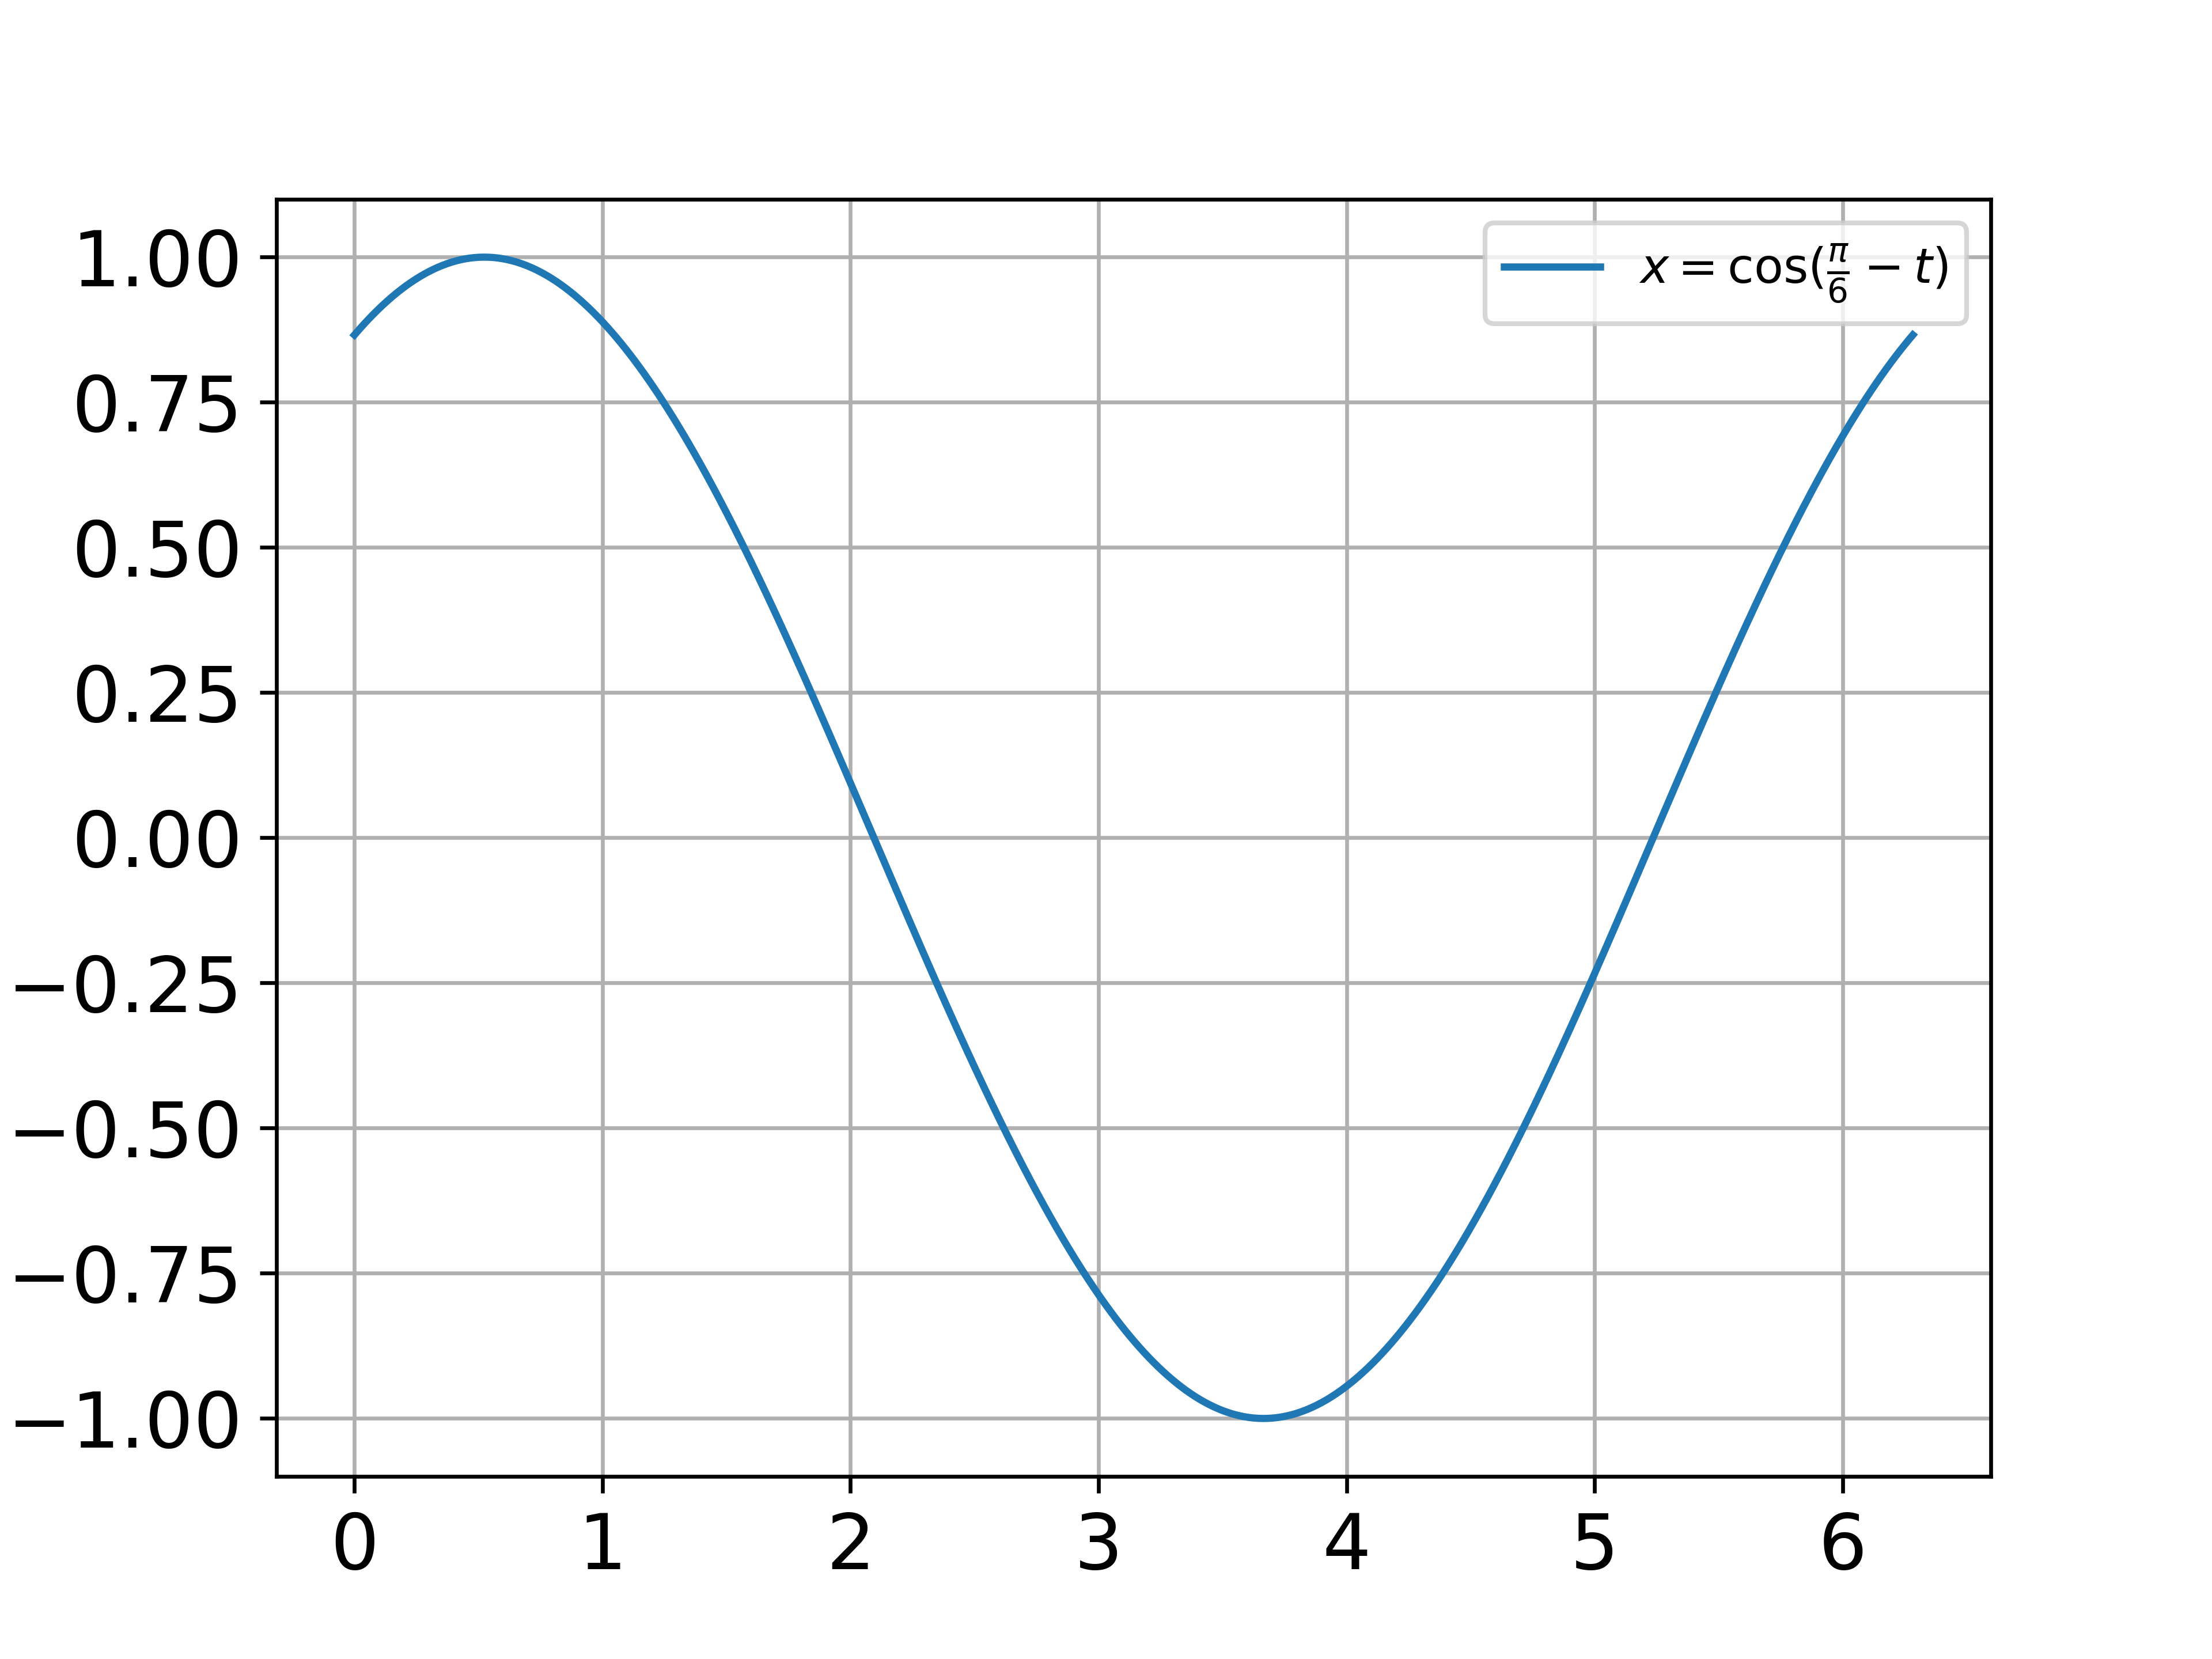
\includegraphics[width=\columnwidth]{ncert-maths/10/5/2/5/figs/Figure_2}
\caption{Plot of $x_2\brak{n}$}
\end{center}
\end{figure}

\end{enumerate}
%\end{document}



\item For what value of $ n$, are the $ nth$ terms of two A.Ps: 63, 65, 67,\dots and 3, 10, 17,\dots equal?
\solution
\iffalse
\let\negmedspace\undefined
\let\negthickspace\undefined
\documentclass[journal,12pt,twocolumn]{IEEEtran}
\usepackage{cite}
\usepackage{amsmath,amssymb,amsfonts,amsthm}
\usepackage{algorithmic}
\usepackage{graphicx}
\usepackage{textcomp}
\usepackage{xcolor}
\usepackage{txfonts}
\usepackage{listings}
\usepackage{enumitem}
\usepackage{mathtools}
\usepackage{gensymb}
\usepackage{comment}
\usepackage[breaklinks=true]{hyperref}
\usepackage{tkz-euclide}
\usepackage{listings}
\usepackage{gvv}
\def\inputGnumericTable{}
\usepackage[latin1]{inputenc}
\usepackage{color}
\usepackage{array}
\usepackage{longtable}
\usepackage{calc}
\usepackage{multirow}
\usepackage{hhline}
\usepackage{ifthen}
\usepackage{lscape}

\newtheorem{theorem}{Theorem}[section]
\newtheorem{problem}{Problem}
\newtheorem{proposition}{Proposition}[section]
\newtheorem{lemma}{Lemma}[section]
\newtheorem{corollary}[theorem]{Corollary}
\newtheorem{example}{Example}[section]
\newtheorem{definition}[problem]{Definition}
\newcommand{\BEQA}{\begin{eqnarray}}
\newcommand{\EEQA}{\end{eqnarray}}
\newcommand{\define}{\stackrel{\triangle}{=}}
\theoremstyle{remark}
\newtheorem{rem}{Remark}
\begin{document}

\bibliographystyle{IEEEtran}
\vspace{3cm}

\title{NCERT Discrete 10.5.2 -15}
\author{EE23BTECH11057 - Shakunaveti Sai Sri Ram Varun$^{}$% &lt;-this % stops a space
}
\maketitle
\newpage
\bigskip

\vspace{2cm}
\textbf{Question: }
For what value of $ n$, are the $ nth$ terms of two A.Ps: 63, 65, 67,\dots and 3, 10, 17,\dots equal?\\
\vspace{0.5cm}
\textbf{Solution}:
\fi
\begin{table}[h] 
\centering
\begin{tabular}{|c|c|c|c|}
    \hline
    \textbf{Parameter} & \textbf{Sub-question} & \textbf{Description} & \textbf{Value} \\
    \hline
    \multirow{2}{*}{$x_i\brak{0}$} & $x_1\brak{0}$ & $1^{st}$ term of $1^{st}$ A.P. & 63 \\
    \cline{2-4}
    & $x_2\brak{0}$ & $1^{st}$ term of $2^{nd}$ A.P. & \phantom{0}3 \\
    \hline
    \multirow{2}{*}{$d_i$} & $d_1$ & Common difference of $1^{st}$ A.P. & \phantom{0}2 \\
    \cline{2-4}
    & $d_2$ & Common difference of $2^{nd}$ A.P. & \phantom{0}7 \\
    \hline
\end{tabular}

\caption{input values}
\label{tab: Table10.5.2.15}
\end{table}
\begin{align}
x_i\brak{n} &= x\brak{0}u\brak{n} + dnu\brak{n}\\
X\brak{z} &= \frac{x\brak{0}}{1-z^{-1}} + \frac{dz^{-1}}{\brak{1-z^{-1}}^{2}} \quad |z|>1
\end{align}
\begin{enumerate}
\item
\begin{align}
x_1\brak{n} &= 63u\brak{n} + 2nu\brak{n}\\
%To find $ X_1\brak{z}$:
X_1\brak{z} &= \frac{63}{1-z^{-1}} + \frac{2z^{-1}}{\brak{1-z^{-1}}^{2}}  \quad |z|>1
\end{align}
\item
\begin{align}
x_2\brak{n} &= 3u\brak{n} + 7nu\brak{n}\\ 
%To find $ X_2\brak{z}$ :\\
X_2\brak{z} &= \frac{3}{1-z^{-1}} + \frac{7z^{-1}}{\brak{1-z^{-1}}^{2}} \quad |z|>1
\end{align}
\item

given,
\begin{align}
 x_1\brak{n} &= x_2\brak{n}\\
\therefore 63 + 2n &= 7n+3\\
\implies n &=12
\end{align}
\begin{figure}[h]
    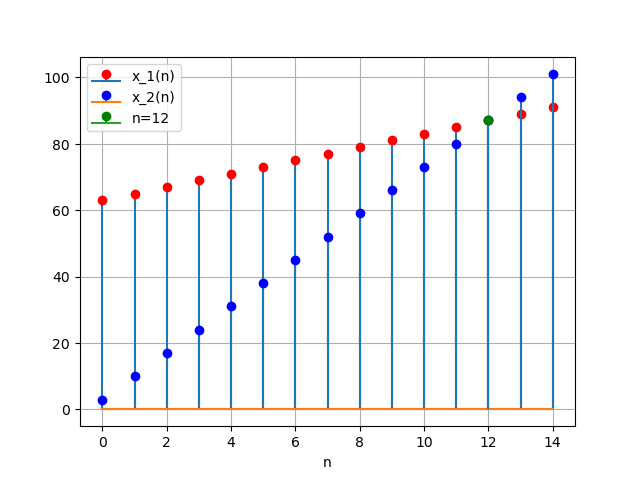
\includegraphics[width = \columnwidth]{ncert-maths/10/5/2/15/figs/Figure_1.png}
    \caption{Graphs of $ x_1\brak{n}$ and $ x_2\brak{n}$ and both are equal at $ n=12$}
    \label{fig: fig10.5.2.15}
\end{figure}
\end{enumerate}
%\end{document}



\item Two APs have the same common difference.The difference between their $100${th} terms is 100,what is the difference between their $1000${th} terms?

\solution
\iffalse
\let\negmedspace\undefined
\let\negthickspace\undefined
\documentclass[journal,12pt,onecolumn]{IEEEtran}
\usepackage{cite}
\usepackage{amsmath,amssymb,amsfonts,amsthm}
\usepackage{algorithmic}
\usepackage{graphicx}
\usepackage{textcomp}
\usepackage{xcolor}
\usepackage{txfonts}
\usepackage{listings}
\usepackage{enumitem}
\usepackage{mathtools}
\usepackage{gensymb}
\usepackage{comment}
\usepackage[breaklinks=true]{hyperref}
\usepackage{tkz-euclide} 
\usepackage{listings}
\usepackage{gvv}                                        
\def\inputGnumericTable{}                                 
\usepackage[latin1]{inputenc}                                
\usepackage{color}                                            
\usepackage{array}                                            
\usepackage{longtable}                                       
\usepackage{calc}                                             
\usepackage{multirow}                                         
\usepackage{hhline}                                           
\usepackage{ifthen}                                           
\usepackage{lscape}
\newtheorem{theorem}{Theorem}[section]
\newtheorem{problem}{Problem}
\newtheorem{proposition}{Proposition}[section]
\newtheorem{lemma}{Lemma}[section]
\newtheorem{corollary}[theorem]{Corollary}
\newtheorem{example}{Example}[section]
\newtheorem{definition}[problem]{Definition}
\newcommand{\BEQA}{\begin{eqnarray}}
\newcommand{\EEQA}{\end{eqnarray}}
\newcommand{\define}{\stackrel{\triangle}{=}}
\theoremstyle{remark}
\newtheorem{rem}{Remark}
\begin{document}
\bibliographystyle{IEEEtran}
\vspace{3cm}
\title{NCERT 11.9.2 16Q}
\author{EE23BTECH11021 - GANNE GOPI CHANDU$^{*}$% <-this % stops a space
}
\maketitle
\bigskip
\renewcommand{\thefigure}{\theenumi}
\renewcommand{\thetable}{\theenumi}
\bibliographystyle{IEEEtran}
\textbf{Question}\\
Between 1 and 31, m numbers have been inserted in such a way that the resulting sequence is an A.P. and 
the ratio of 7 th and (m - 1) th numbers is 5:9. Find the value of m.\\
\textbf{Solution}\\
\fi
\begin{table}[!h]
\begin{center}
\renewcommand\thetable{1}
\begin{tabular}{ |c|c|c| } 
  \hline
    Symbol & Value & description \\ 
  \hline
  $x(0)$ & $1$ & First term of A.P  \\ 
  \hline
  $x(n)$ & $31$ & $\brak{n+1}\text{th}$ term \\
  \hline
  $\frac{x\brak{7}}{x\brak{m-1}}$ & $\frac{5}{9}$ & ratio of $7$ th  and $(m-1)$ th numbers\\ 
  \hline
  $n$ & $m+2$ & number of terms \\
  \hline
\end{tabular}
\end{center}
\caption{}
\end{table}\\
The last term is
\begin{align}
x(n)&=x(0)+\brak{n}d\\
\implies31 &= 1 + \brak{m + 1}d \\
\implies30 &= \brak{m + 1}d \\
\implies\frac{30}{m + 1} &= d \label{eq11.9.2.4}
\end{align}
Now $7$th and $\brak{m-1}$th terms
\begin{align}
x\brak{7} &= x(0) + 7d\label{eq11.9.2.5}\\
x\brak{m-1} &= x(0) + \brak{m-1}d\label{eq11.9.2.6}
\end{align}
From  equations \eqref{eq11.9.2.5} and \eqref{eq11.9.2.6}\\
\begin{align}
   \frac{x(0) + 7d}{x(0) + \brak{m-1}d} &= \frac{5}{9} \label{eq11.9.2.7}
\end{align}
Substituting  \eqref{eq11.9.2.4} in \eqref{eq11.9.2.7}\\
\begin{align}
\implies \frac{1+7\brak{{\frac{30}{m+1}}}}{1+\brak{{m-1}}\brak{\frac{30}{m+1}}} &= \frac{5}{9} \\
\implies \frac{m+1+210}{m+1+30m-30} &= \frac{5}{9}\\
\implies \frac{m+181}{31m-29} &= \frac{5}{9}\\
\implies 9m+1899 &=155m-145\\
\implies 155m-9m &=1899+145\\
\implies 146m &=2044\\
\implies m &=14
\end{align}
Therefore, $m = 14$ .\\
 \text{General term of AP is} \\
\begin{align}
    x\brak{n}&=\brak{2n+1}u(n)\\
    x\brak{n}&=\brak{2n}u\brak{n}+u\brak{n}
\end{align}
\begin{figure}
    \centering
    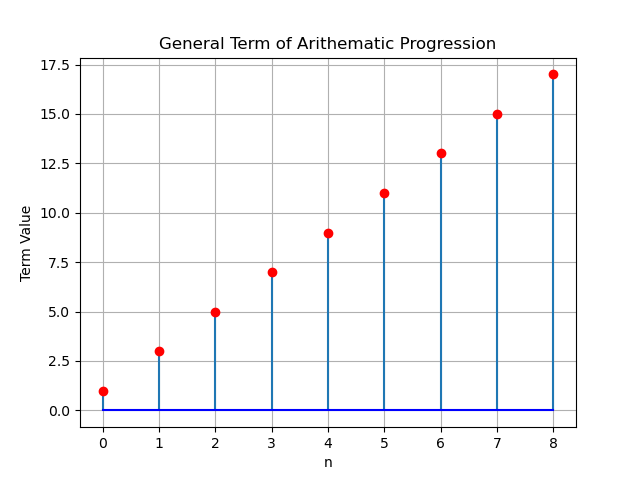
\includegraphics[width=1.0\linewidth]{ncert-maths/11/9/2/16/figs/test.png}
    \caption{Plot of x(n) vs n}
    \label{fig:1}
\end{figure}\\
The Z-Transform is\\
\begin{align}
    X\brak{z}&=2\brak{\dfrac{z}{\brak{z-1}^{2}}}+U\brak{z}\\
    &=\dfrac{2z}{\brak{z-1}^{2}}+\dfrac{1}{1-z^{-1}}\\
    X\brak{z}&=\dfrac{z^2+z}{\brak{z-1}^{2}} \quad{|z|>1}
\end{align}


\item Check whether -150 is a term of the AP: 11,8,5,2,....

 \solution
 \iffalse
\let\negmedspace\undefined
\let\negthickspace\undefined
\documentclass[journal,12pt,onecolumn]{IEEEtran}
\usepackage{cite}
\usepackage{amsmath,amssymb,amsfonts,amsthm}
\usepackage{algorithmic}
\usepackage{graphicx}
\usepackage{textcomp}
\usepackage{xcolor}
\usepackage{txfonts}
\usepackage{listings}
\usepackage{enumitem}
\usepackage{mathtools}
\usepackage{gensymb}
\usepackage{comment}
\usepackage[breaklinks=true]{hyperref}
\usepackage{tkz-euclide} % loads  TikZ and tkz-base
\usepackage{listings}
\usepackage[latin1]{inputenc}                                
\usepackage{color}                                            
\usepackage{array}                                            
\usepackage{longtable}                                       
\usepackage{calc}                                             
\usepackage{multirow}                                         
\usepackage{hhline}                                           
\usepackage{ifthen}                                           
\usepackage{lscape}
\usepackage{caption}


\newtheorem{theorem}{Theorem}[section]
\newtheorem{problem}{Problem}
\newtheorem{proposition}{Proposition}[section]
\newtheorem{lemma}{Lemma}[section]
\newtheorem{corollary}[theorem]{Corollary}
\newtheorem{example}{Example}[section]
\newtheorem{definition}[problem]{Definition}
%\newtheorem{thm}{Theorem}[section] 
%\newtheorem{defn}[thm]{Definition}
%\newtheorem{algorithm}{Algorithm}[section]
%\newtheorem{cor}{Corollary}
\newcommand{\BEQA}{\begin{eqnarray}}
\newcommand{\EEQA}{\end{eqnarray}}
\newcommand{\define}{\stackrel{\triangle}{=}}
\theoremstyle{remark}
\newtheorem{rem}{Remark}
%\bibliographystyle{ieeetr}

\begin{document}

%
\providecommand{\pr}[1]{\ensuremath{\Pr\left(#1\right)}}
\providecommand{\prt}[2]{\ensuremath{p_{#1}^{\left(#2\right)} }}        % own macro for this question
\providecommand{\qfunc}[1]{\ensuremath{Q\left(#1\right)}}
\providecommand{\sbrak}[1]{\ensuremath{{}\left[#1\right]}}
\providecommand{\lsbrak}[1]{\ensuremath{{}\left[#1\right.}}
\providecommand{\rsbrak}[1]{\ensuremath{{}\left.#1\right]}}
\providecommand{\brak}[1]{\ensuremath{\left(#1\right)}}
\providecommand{\lbrak}[1]{\ensuremath{\left(#1\right.}}
\providecommand{\rbrak}[1]{\ensuremath{\left.#1\right)}}
\providecommand{\cbrak}[1]{\ensuremath{\left\{#1\right\}}}
\providecommand{\lcbrak}[1]{\ensuremath{\left\{#1\right.}}
\providecommand{\rcbrak}[1]{\ensuremath{\left.#1\right\}}}
\newcommand{\sgn}{\mathop{\mathrm{sgn}}}
\providecommand{\abs}[1]{\left\vert#1\right\vert}
\providecommand{\res}[1]{\Res\displaylimits_{#1}} 
\providecommand{\norm}[1]{\left\lVert#1\right\rVert}
%\providecommand{\norm}[1]{\lVert#1\rVert}
\providecommand{\mtx}[1]{\mathbf{#1}}
\providecommand{\mean}[1]{E\left[ #1 \right]}
\providecommand{\cond}[2]{#1\middle|#2}
\providecommand{\fourier}{\overset{\mathcal{F}}{ \rightleftharpoons}}
\newenvironment{amatrix}[1]{%
  \left(\begin{array}{@{}*{#1}{c}|c@{}}
}{%
  \end{array}\right)
}
%\providecommand{\hilbert}{\overset{\mathcal{H}}{ \rightleftharpoons}}
%\providecommand{\system}{\overset{\mathcal{H}}{ \longleftrightarrow}}
        %\newcommand{\solution}[2]{\textbf{Solution:}{#1}}
\newcommand{\solution}{\noindent \textbf{Solution: }}
\newcommand{\cosec}{\,\text{cosec}\,}
\providecommand{\dec}[2]{\ensuremath{\overset{#1}{\underset{#2}{\gtrless}}}}
\newcommand{\myvec}[1]{\ensuremath{\begin{pmatrix}#1\end{pmatrix}}}
\newcommand{\mydet}[1]{\ensuremath{\begin{vmatrix}#1\end{vmatrix}}}
\newcommand{\myaugvec}[2]{\ensuremath{\begin{amatrix}{#1}#2\end{amatrix}}}
\providecommand{\rank}{\text{rank}}
\providecommand{\pr}[1]{\ensuremath{\Pr\left(#1\right)}}
\providecommand{\qfunc}[1]{\ensuremath{Q\left(#1\right)}}
        \newcommand*{\permcomb}[4][0mu]{{{}^{#3}\mkern#1#2_{#4}}}
\newcommand*{\perm}[1][-3mu]{\permcomb[#1]{P}}
\newcommand*{\comb}[1][-1mu]{\permcomb[#1]{C}}
\providecommand{\qfunc}[1]{\ensuremath{Q\left(#1\right)}}
\providecommand{\gauss}[2]{\mathcal{N}\ensuremath{\left(#1,#2\right)}}
\providecommand{\diff}[2]{\ensuremath{\frac{d{#1}}{d{#2}}}}
\providecommand{\myceil}[1]{\left \lceil #1 \right \rceil }
\newcommand\figref{Fig.~\ref}
\newcommand\tabref{Table~\ref}
\newcommand{\sinc}{\,\text{sinc}\,}
\newcommand{\rect}{\,\text{rect}\,}
%%
%       %\newcommand{\solution}[2]{\textbf{Solution:}{#1}}
%\newcommand{\solution}{\noindent \textbf{Solution: }}
%\newcommand{\cosec}{\,\text{cosec}\,}
%\numberwithin{equation}{section}
%\numberwithin{equation}{subsection}
%\numberwithin{problem}{section}
%\numberwithin{definition}{section}
%\makeatletter
%\@addtoreset{figure}{problem}
%\makeatother

%\let\StandardTheFigure\thefigure
\let\vec\mathbf

\bibliographystyle{IEEEtran}

\vspace{3cm}
\title{Assignment}
\author{EE23BTECH11001 - Aashna Sahu}
\maketitle
\bigskip

\renewcommand{\thefigure}{\theenumi}
\renewcommand{\thetable}{\theenumi}
%\renewcommand{\theequation}{\theenumi}
Q:Check whether -150 is a term of the AP: 11,8,5,2,....

 \solution
 \fi

\begin{align}
x(n)&=x(0)+nd\\
n&=\frac{x(n)-x(0)}{d}
\end{align}
\begin{align}
x(n)-x(0) &\equiv 0 \pmod{d}
\end{align}
On substitutings values\\
\begin{align}
-161 &\equiv 2 \pmod{-3}
\end{align}
Thus -150 is not a term of the given AP.
\begin{align}
 \boxed{x(n)=(11-3n)\times u(n)}   
\end{align}

\begin{align}
   X(z)&=\frac{11}{1-z^{-1}}-\frac{3z^{-1}}{(1-z^{-1})^2}\quad
    |z|>1
\end{align}

    \begin{table}[h]
    \centering
    
        \begin{tabular}{|c|c|c|}
	\hline
	\textbf{Symbol} & \textbf{Value} & \textbf{Description} \\[6pt]
	\hline
	$x(0)$ & $25$ & first term of AP \\[6pt]
	\hline
	$d$ & $-3$ & common difference \\[6pt]
	\hline
	$x(n)$ & $(25-3n)u(n)$ & $n$-th term of AP \\[6pt]
	\hline
	$y(n)$ & $116$ & sum of terms \\[6pt]
	\hline 
\end{tabular}

        
    \caption{Input parameters}
    \label{tab:Table10.5.2.6}
\end{table}
\newpage
\begin{figure}[h]
  \centering
  \includegraphics[width=1.2\columnwidth]{ncert-maths/10/5/2/6/figs/Figure_1.png}
  \caption{Representation of x(n)}
  \label{fig:fig10.5.2.6}
\end{figure}
%\end{document}

 

 \item Write the first five terms of the sequence \(a_n = \frac{n(n^2+5)}{4}\).

\solution
\input{ncert-maths/11/9/1/6/file1.tex}


\item
\begin{enumerate}
\item 30th term of the AP: 10, 7, 4, $\ldots$ is 
\item 11th term of the AP: $-3, -\frac{1}{2}, 2, \ldots$ is
\end{enumerate}
\solution
\input{ncert-maths/10/5/2/2/c.tex}


\item Write the first five terms of the sequence whose nth term is $\frac{2n-3}{6}$ and obtain the Z transform of the series
\solution
\input{ncert-maths/11/9/1/4/d.tex}

 \item For what values of x, the numbers $-\frac{2}{7}\,,x,-\frac{7}{2}\,$ are in G.P ?

\solution
\iffalse
\let\negmedspace\undefined
\let\negthickspace\undefined
\documentclass[journal,12pt,twocolumn]{IEEEtran}
\usepackage{cite}
\usepackage{amsmath,amssymb,amsfonts,amsthm}
\usepackage{algorithmic}
\usepackage{graphicx}
\usepackage{textcomp}
\usepackage[justification=centering]{caption}
\usepackage{xcolor}
\usepackage{txfonts}
\usepackage{listings}
\usepackage{enumitem}
\usepackage{mathtools}
\usepackage{gensymb}
\usepackage{comment}
\usepackage[breaklinks=true]{hyperref}
\usepackage{tkz-euclide} 
\usepackage{listings}
\usepackage{gvv}                                        
\def\inputGnumericTable{}                                 
\usepackage[latin1]{inputenc}                                
\usepackage{color}                                            
\usepackage{array}                                            
\usepackage{longtable}                                       
\usepackage{calc}                                             
\usepackage{multirow}                                         
\usepackage{hhline}                                           
\usepackage{ifthen}                                           
\usepackage{lscape}

\newtheorem{theorem}{Theorem}[section]
\newtheorem{problem}{Problem}
\newtheorem{proposition}{Proposition}[section]
\newtheorem{lemma}{Lemma}[section]
\newtheorem{corollary}[theorem]{Corollary}
\newtheorem{example}{Example}[section]
\newtheorem{definition}[problem]{Definition}
\newcommand{\BEQA}{\begin{eqnarray}}
\newcommand{\EEQA}{\end{eqnarray}}
\newcommand{\define}{\stackrel{\triangle}{=}}
\theoremstyle{remark}
\newtheorem{rem}{Remark}
\begin{document}

\bibliographystyle{IEEEtran}
\vspace{3cm}

\title{11.9.3.6}
\author{EE23BTECH11022 - G DILIP REDDY}
\maketitle
\newpage

\bigskip

\renewcommand{\thefigure}{\theenumi}
\renewcommand{\thetable}{\theenumi}
\textbf{Question}:\\
For what values of x, the numbers $-\frac{2}{7}\,,x,-\frac{7}{2}\,$ are in G.P ?
\\\\
\textbf{Solution: }\\
\fi
\begin{table}[h]
    \centering
    \renewcommand\thetable{1}
    \begin{tabular}[12.1pt]{ |c| c| c|}
    \hline
    \textbf{Variable} & \textbf{Description} &\textbf{Value}\\ 
    \hline
    $x(0)$ & First term of the GP &$-\brak{\frac{2}{7}}$ \\
    \hline 
    $x(1)$ & Second term of the GP &$x$ \\
    \hline 
    $x(2)$ & Third term of the GP &$-\brak{\frac{7}{2}}$ \\
    \hline 
    $r$ & Common ratio of the GP & \\
    \hline
    $x(n)$ & General term & $x(0)\,r^n\,u(n)$\\
    \hline    
\end{tabular}

    \caption{Variables Used}
    \label{tab:table_11.9.3.6}
\end{table}
Let $r$ be the common ratio\\
From \tabref{tab:table_11.9.3.6}:
\begin{align}
\implies \frac{x}{\brak{-\frac{2}{7}\,}}\,&= \frac{\brak{-\frac{7}{2}\,}}{x}\,=r \\
x^2&=\brak{-\frac{2}{7}\,}\cdot\brak{-\frac{7}{2}\,}\\
x&=\pm 1\\
\implies r&=\pm \frac{7}{2}\,\\\notag
\end{align}
The signal corresponding to this is 
\begin{align}
x(n)=\brak{-\frac{2}{7}}\brak{\pm \frac{7}{2}}^n\,u(n)
\end{align}
Applying z-Transform :
\begin{align}
\implies X_1(z)&=\brak{\frac{1}{7}}\brak{\frac{4}{7z^{-1}+2}\,}
\quad \abs{z}>\frac{7}{2}\\
\implies X_2(z)&=\brak{\frac{1}{7}}\brak{\frac{4}{7z^{-1}-2}\,}
\quad \abs{z}>\frac{7}{2}
\end{align}
\begin{figure}[h]
    \renewcommand\thefigure{1}
    \centering
    \captionsetup{justification=centering}
    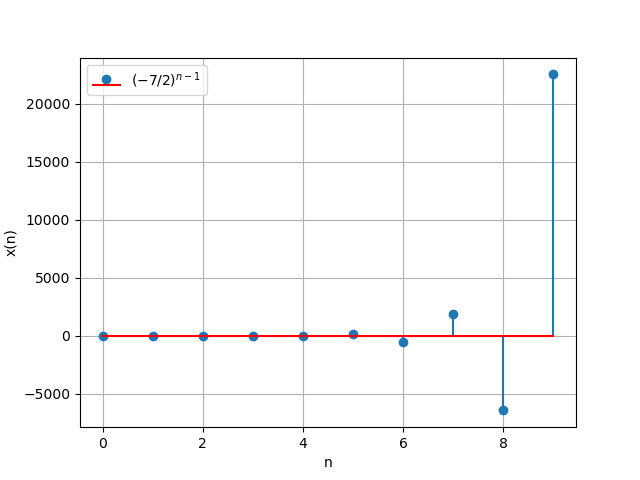
\includegraphics[width=1.1\linewidth]{ncert-maths/11/9/3/6/figs/graph1.png}
    \caption{Stem Plot of $x_1$(n)}
    \label{stemplot1}
\end{figure}
\begin{figure}[h]
    \renewcommand\thefigure{2}
    \centering
    \captionsetup{justification=centering}
    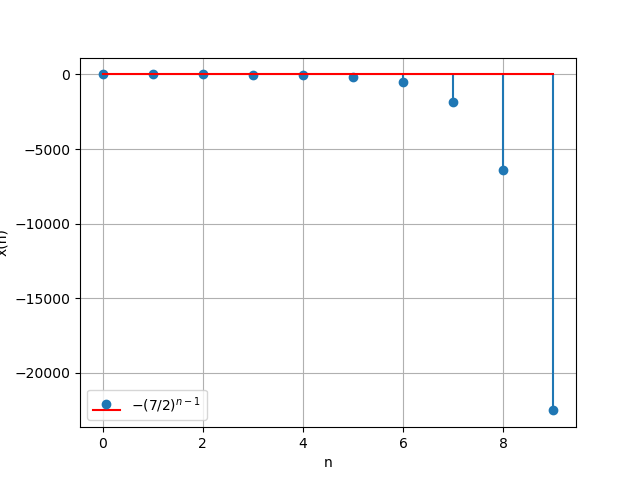
\includegraphics[width=1.1\linewidth]{ncert-maths/11/9/3/6/figs/graph2.png}
    \caption{Stem Plot of $x_2(n)$}
    \label{stemplot2}
\end{figure}
%\end{document}



\item Find the $20^{th}$ and $n^{th}$ terms of the G.P $\frac{5}{2}$, $\frac{5}{4}$, $\frac{5}{8}$,.....

\solution
% \iffalse
\let\negmedspace\undefined
\let\negthickspace\undefined
\documentclass[journal,12pt,twocolumn]{IEEEtran}
\usepackage{cite}
\usepackage{amsmath,amssymb,amsfonts,amsthm}
\usepackage{algorithmic}
\usepackage{graphicx}
\usepackage{textcomp}
\usepackage{xcolor}
\usepackage{txfonts}
\usepackage{listings}
\usepackage{enumitem}
\usepackage{mathtools}
\usepackage{gensymb}
\usepackage{comment}
\usepackage[breaklinks=true]{hyperref}
\usepackage{tkz-euclide} 
\usepackage{listings}
\usepackage{gvv}                                        
\def\inputGnumericTable{}                                 
\usepackage[latin1]{inputenc}                                
\usepackage{color}                                            
\usepackage{array}                                            
\usepackage{longtable}                                       
\usepackage{calc}                                             
\usepackage{multirow}                                         
\usepackage{hhline}                                           
\usepackage{ifthen}                                           
\usepackage{lscape}
\usepackage{caption}
\newtheorem{theorem}{Theorem}[section]
\newtheorem{problem}{Problem}
\newtheorem{proposition}{Proposition}[section]
\newtheorem{lemma}{Lemma}[section]
\newtheorem{corollary}[theorem]{Corollary}
\newtheorem{example}{Example}[section]
\newtheorem{definition}[problem]{Definition}
\newcommand{\BEQA}{\begin{eqnarray}}
\newcommand{\EEQA}{\end{eqnarray}}
\newcommand{\define}{\stackrel{\triangle}{=}}
\theoremstyle{remark}
\newtheorem{rem}{Remark}
\begin{document}
\parindent 0px
\bibliographystyle{IEEEtran}
\vspace{3cm}

\title{NCERT 11.9.3 1Q}
\author{EE23BTECH11013 - Avyaaz$^{*}$% <-this % stops a space
}
\maketitle
\newpage
\bigskip

\renewcommand{\thefigure}{\arabic{figure}}
\renewcommand{\thetable}{\arabic{table}}
\large\textbf{\textsl{Question:}}
Find the $20^{th}$ and $n^{th}$ terms of the G.P $\frac{5}{2}$, $\frac{5}{4}$, $\frac{5}{8}$,.....

\solution
 \begin{table}[htbp]
     \centering
     \setlength{\extrarowheight}{8pt}
    \begin{tabular}{|c|c|c|}
	\hline
	\textbf{Symbol} & \textbf{Value} & \textbf{Description} \\[6pt]
	\hline
	$x(0)$ & $25$ & first term of AP \\[6pt]
	\hline
	$d$ & $-3$ & common difference \\[6pt]
	\hline
	$x(n)$ & $(25-3n)u(n)$ & $n$-th term of AP \\[6pt]
	\hline
	$y(n)$ & $116$ & sum of terms \\[6pt]
	\hline 
\end{tabular}

     \caption{Parameters}
     \label{tab:table1}
 \end{table} 

% \begin{align}
%    x(n) = \dfrac{5}{2}\left(\dfrac{1}{2}\right)^n 
% \end{align}

% \begin{align}
% 	x \brak{n} & \system{Z} X \brak{z} \\
%    % x(n) &=\dfrac{5}{2}\left(\dfrac{1}{2}\right)^n u(n) \\
%     \therefore X(z) &= \sum_{n=-\infty}^{\infty}x(n)z^{-n}\label{eq:z-transform}  
% \end{align}
% Here, 
%          $    u(n) = \begin{cases}
%                 0 &\text{for } n < 0 \\
%                 1 & \text{for } n \geq 0
%             \end{cases}$       
 
%  \vspace{1cm}
From \tabref{tab:table1}:
\(Z\)-Transform of \(x(n)\):
\begin{align}
% \implies X(z) &= \sum_{n=-\infty}^{\infty}\left(\dfrac{5}{2}\left(\dfrac{1}{2}\right)^n u(n)\right) z^{-n} \\
 % \implies X(z) &= \dfrac{5}{2}\sum_{n=0}^{\infty}\left(\dfrac{z
 % ^{-1}}{2}\right)^n \\
\implies X(z) &=\dfrac{5}{2}\left(\dfrac{1}{1-\frac{z^{-1}}{2}}\right) ;\cbrak{z\in\mathbb{C} : |z|>\dfrac{1}{2}}
\end{align}

\begin{figure}[ht]
    \centering
    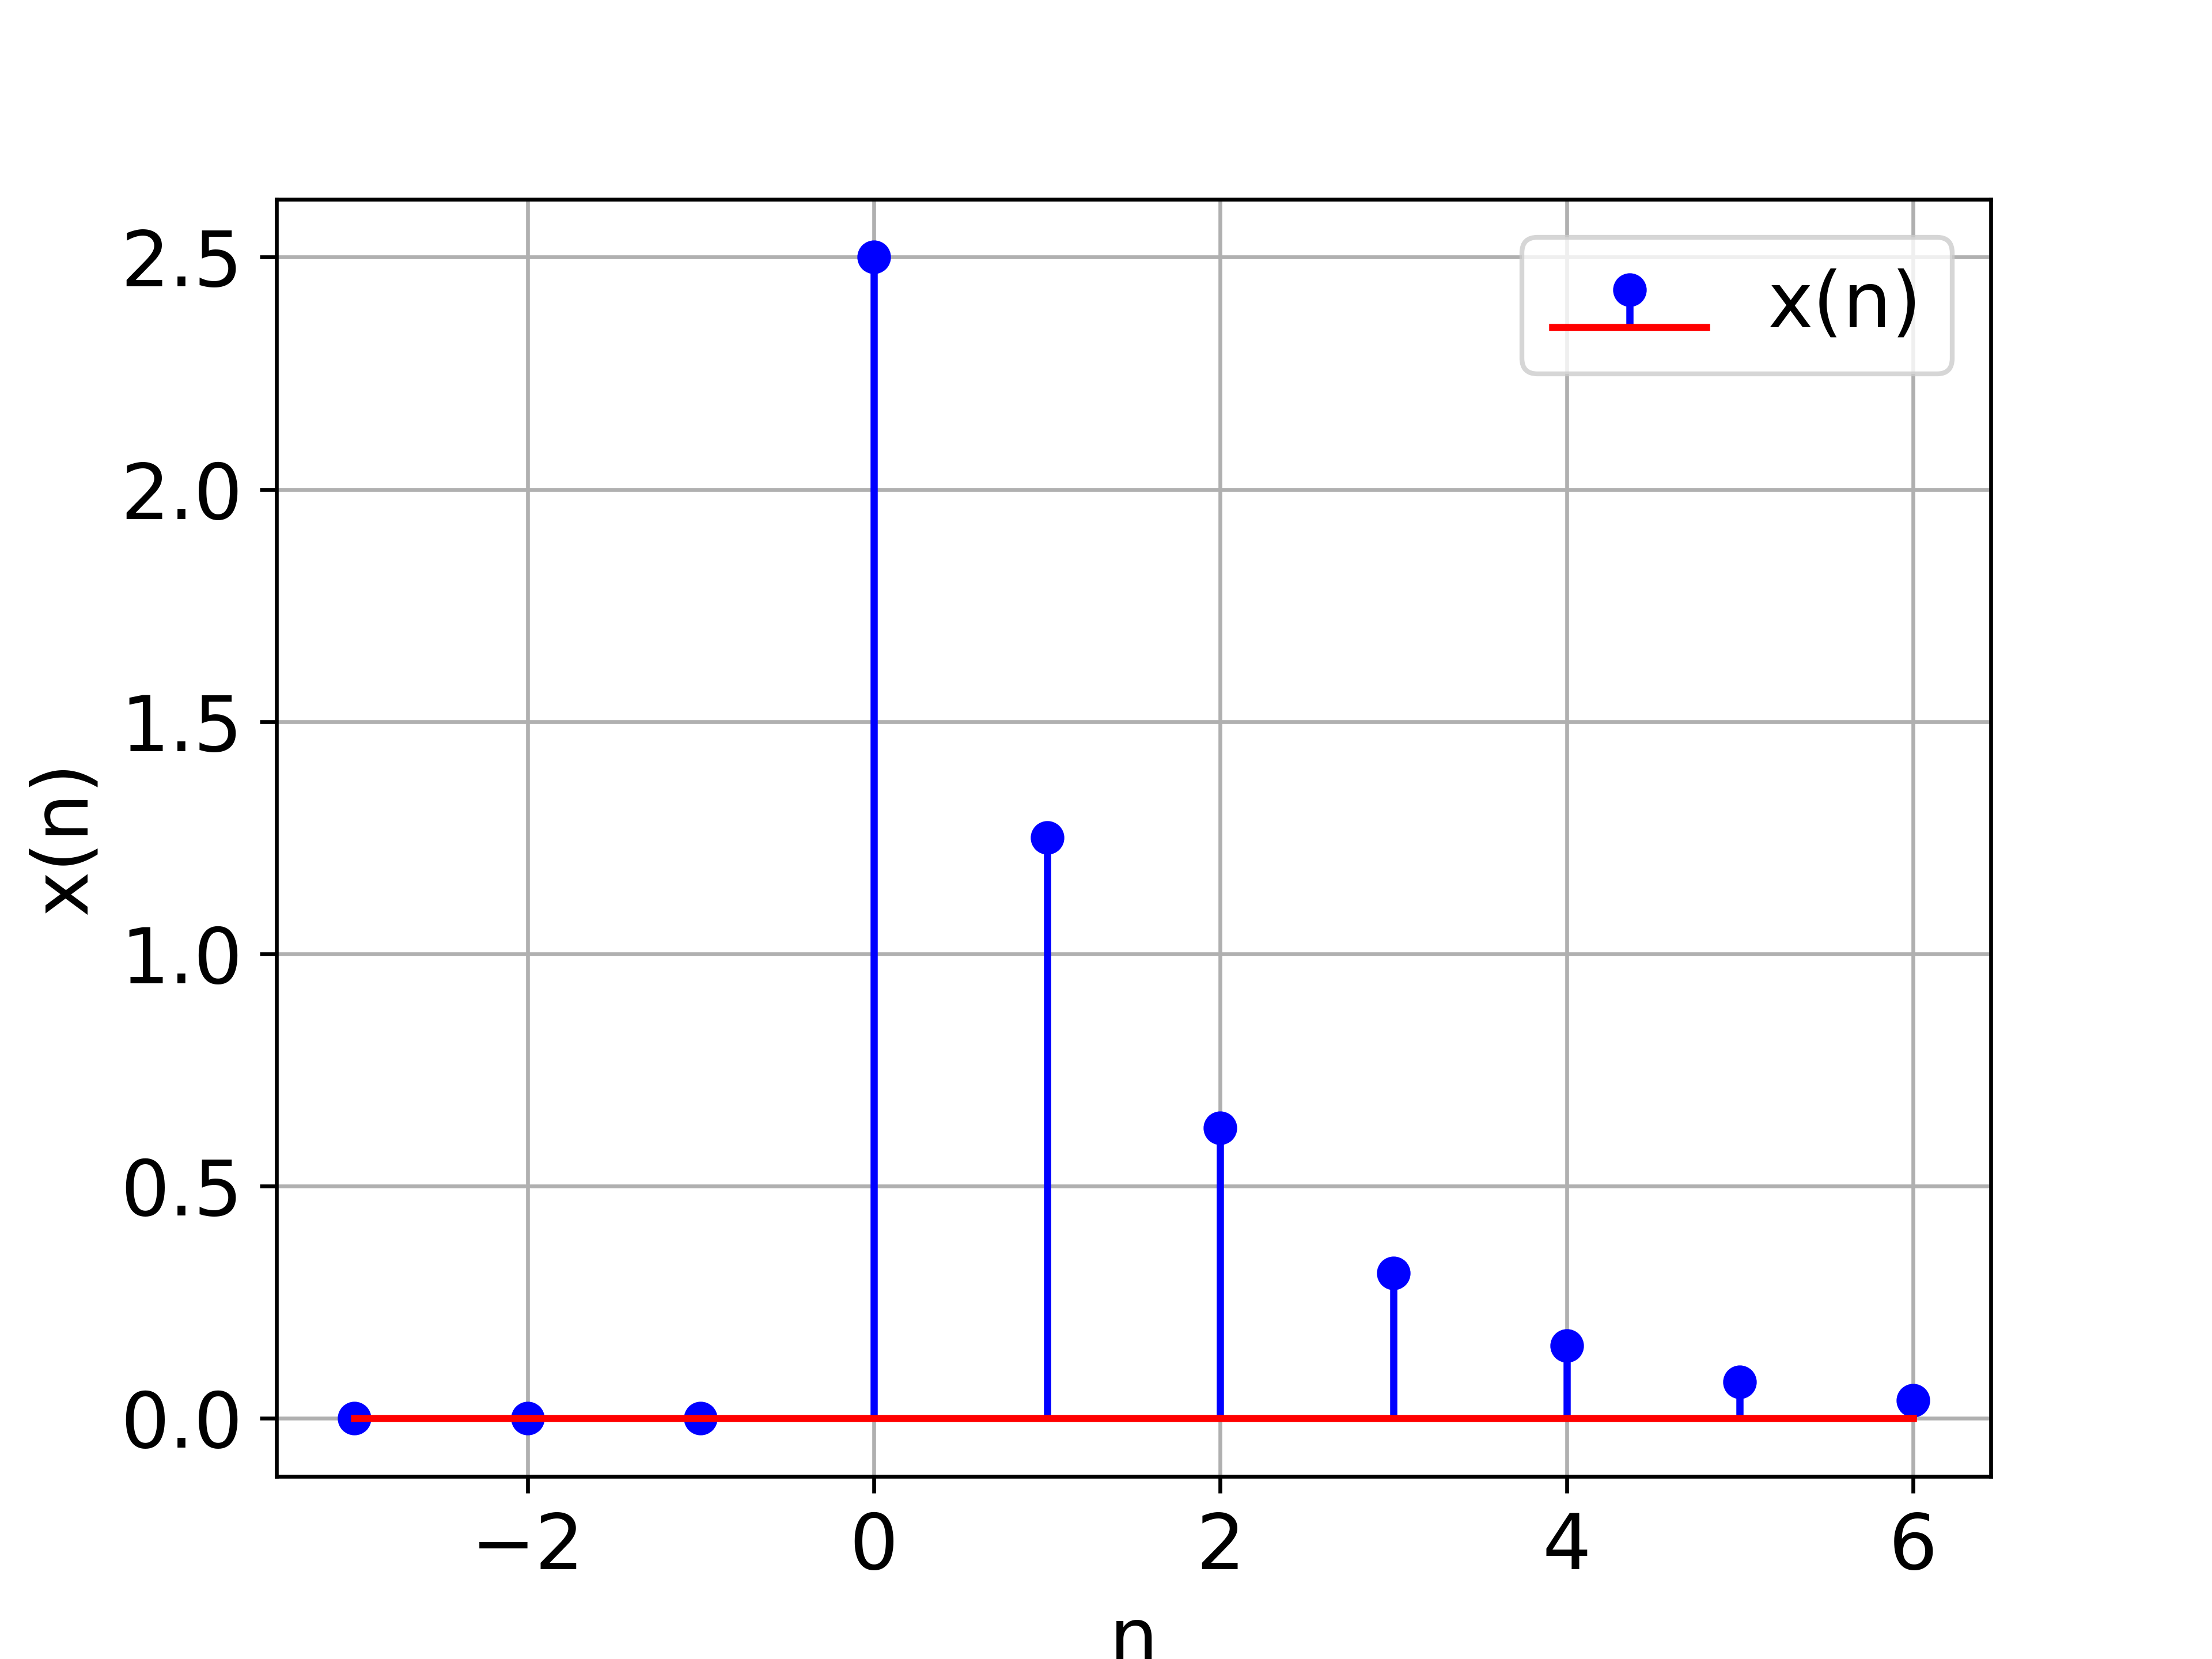
\includegraphics[width = \columnwidth]{figs/stem_plot.png}
    \caption{}
    \label{fig:graph1}
\end{figure} 

\bibliographystyle{IEEEtran}
\end{document}



\item 
Which term of the following sequences:\\
(a) 2,$2\sqrt{2}$,4\dots is 128
\quad(b) $\sqrt{3}$,3,$3\sqrt{3}$\dots is 729\\
(c) $\frac{1}{3}$,$\frac{1}{9}$,$\frac{1}{27}$\dots is $\frac{1}{19683}$ \\
\solution
\iffalse
\let\negmedspace\undefined
\let\negthickspace\undefined
\documentclass[journal,12pt,twocolumn]{IEEEtran}
\usepackage{cite}
\usepackage{amsmath,amssymb,amsfonts,amsthm}
\usepackage{algorithmic}
\usepackage{graphicx}
\usepackage{textcomp}
\usepackage{xcolor}
\usepackage{txfonts}
\usepackage{listings}
\usepackage{enumitem}
\usepackage{mathtools}
\usepackage{gensymb}
\usepackage{comment}
\usepackage[breaklinks=true]{hyperref}
\usepackage{tkz-euclide} 
\usepackage{listings}
\usepackage{gvv}                                        
\def\inputGnumericTable{}                                 
\usepackage[latin1]{inputenc}                                
\usepackage{color}                                            
\usepackage{array}                                            
\usepackage{longtable}                                       
\usepackage{calc}                                             
\usepackage{multirow}                                         
\usepackage{hhline}                                           
\usepackage{ifthen}                                           
\usepackage{lscape}
\usepackage[center]{caption} % center the captions to figure

\newtheorem{theorem}{Theorem}[section]
\newtheorem{problem}{Problem}
\newtheorem{proposition}{Proposition}[section]
\newtheorem{lemma}{Lemma}[section]
\newtheorem{corollary}[theorem]{Corollary}
\newtheorem{example}{Example}[section]
\newtheorem{definition}[problem]{Definition}
\newcommand{\BEQA}{\begin{eqnarray}}
\newcommand{\EEQA}{\end{eqnarray}}
\newcommand{\define}{\stackrel{\triangle}{=}}
\theoremstyle{remark}
\newtheorem{rem}{Remark}
\begin{document}

\newcolumntype{M}[1]{>{\centering\arraybackslash}m{#1}}
\newcolumntype{N}{@{}m{0pt}@{}}

\bibliographystyle{IEEEtran}
\vspace{3cm}

\title{NCERT 11.9.3 5Q} 
\author{ee23btech11223 - Soham Prabhakar More% <-this % stops a space
}
\maketitle
\newpage
\bigskip

\renewcommand{\thefigure}{\theenumi}
\renewcommand{\thetable}{\theenumi}

\bibliographystyle{IEEEtran}

\textbf{Question:}\\
Which term of the following sequences:\\
(a) 2,$2\sqrt{2}$,4\dots is 128
\quad(b) $\sqrt{3}$,3,$3\sqrt{3}$\dots is 729\\
(c) $\frac{1}{3}$,$\frac{1}{9}$,$\frac{1}{27}$\dots is $\frac{1}{19683}$
\fi 
For a general GP series and $k > 0$,
\begin{align}
    x\brak{k} &= x\brak{0}r^k \\
    \therefore k &= \log_r{\frac{x\brak{k}}{x\brak{0}}} \label{eq:gsoln}
\end{align}
And the Z-transform $X\brak{z}$:
\begin{align}
    X\brak{z} &= \frac{x\brak{0}}{1 - rz^{-1}} \quad {\abs{z} > \abs{r}} \label{eq:zresult}
\end{align}

\begin{enumerate}[label=(\alph*)]
\item By \tabref{Table:1}, \eqref{eq:gsoln} and \tabref{Table:1}: % prob:a
\begin{align}
    x_1\brak{n} &= x_1\brak{0} r_1^nu\brak{n} \\
    k_1 &= \log_{r_1}{\frac{128}{x_1\brak{0}}} \\
    \therefore k_1 &= 12 \\
	X_1\brak{z} &= \frac{2}{1 - \sqrt{2}z^{-1}} \quad \abs{z} > \sqrt{2}
\end{align}

\begin{figure}[h!]
    \renewcommand\thefigure{1}
    \centering
    \includegraphics[width=\columnwidth]{ncert-maths/11/9/3/5/figs/a.png}
    \caption[short]{Plot of $x_1$\brak{n} vs n. See \tabref{Table:1}}
    \label{fig:img1}
\end{figure}



\item By \eqref{eq:gsoln}, \eqref{eq:zresult} and \tabref{Table:1}: % prob:b
\begin{align}
    x_2\brak{n} &= x_2\brak{0} r_2^nu\brak{n} \\
    k_2 &= \log_{r_2}{\frac{729}{x_2\brak{0}}} \\
    \therefore k_2 &= 11 \\
    X_2\brak{z} &= \frac{\sqrt{3}}{1 - \sqrt{3}z^{-1}} \quad \abs{z} > \sqrt{3} 
\end{align}

\begin{figure}[h!]
    \renewcommand\thefigure{2}
    \centering
    \includegraphics[width=\columnwidth]{ncert-maths/11/9/3/5/figs/b.png}
    \caption[short]{Plot of $x_2$\brak{n} vs n. See \tabref{Table:1}}
    \label{fig:img2}
\end{figure}

\item By \eqref{eq:gsoln}, \eqref{eq:zresult} and \tabref{Table:1}: % prob:c
\begin{align}
    x_3\brak{n} &= x_3\brak{0} r_3^nu\brak{n} \\
    k_3 &= \log_{r_3}{\frac{1}{19683 x_3\brak{0}}} \\
    \therefore k_3 &= 8 \\
    X_3\brak{z} &= \frac{1}{3 - z^{-1}} \quad \abs{z} > \frac{1}{3}
\end{align}

\begin{figure}[h!]
    \renewcommand\thefigure{3}
    \centering
    \includegraphics[width=0.9\columnwidth]{ncert-maths/11/9/3/5/figs/c.png}
    \caption[short]{Plot of $x_3$\brak{n} vs n. See \tabref{Table:1}}
    \label{fig:img3}
\end{figure}

\begin{table}[ht]
\begin{tabular}{|l|l|c|}
\hline
\textbf{Symbol} & \textbf{Description} & \textbf{Value} \\
\hline
$x\brak{n}$ & General term & $ar^n$ \\
\hline
$a$ & First term & 1 \\
\hline
$r$ & Common ratio & - \\
\hline
$x\brak{2} + x\brak{4}$ & Sum of 3rd and 5th terms & 90 \\
\hline
\end{tabular}

\end{table}

\end{enumerate}

Find the $20^{th}$ and $n^{th}$ terms of the G.P $\frac{5}{2}$, $\frac{5}{4}$, $\frac{5}{8}$,.....

% \item 
% Which term of the following sequences:\\
% (a) 2,$2\sqrt{2}$,4\dots is 128
% \quad(b) $\sqrt{3}$,3,$3\sqrt{3}$\dots is 729\\
% (c) $\frac{1}{3}$,$\frac{1}{9}$,$\frac{1}{27}$\dots is $\frac{1}{19683}$ \\
% \solution
% \iffalse
\let\negmedspace\undefined
\let\negthickspace\undefined
\documentclass[journal,12pt,twocolumn]{IEEEtran}
\usepackage{cite}
\usepackage{amsmath,amssymb,amsfonts,amsthm}
\usepackage{algorithmic}
\usepackage{graphicx}
\usepackage{textcomp}
\usepackage{xcolor}
\usepackage{txfonts}
\usepackage{listings}
\usepackage{enumitem}
\usepackage{mathtools}
\usepackage{gensymb}
\usepackage{comment}
\usepackage[breaklinks=true]{hyperref}
\usepackage{tkz-euclide} 
\usepackage{listings}
\usepackage{gvv}                                        
\def\inputGnumericTable{}                                 
\usepackage[latin1]{inputenc}                                
\usepackage{color}                                            
\usepackage{array}                                            
\usepackage{longtable}                                       
\usepackage{calc}                                             
\usepackage{multirow}                                         
\usepackage{hhline}                                           
\usepackage{ifthen}                                           
\usepackage{lscape}
\usepackage[center]{caption} % center the captions to figure

\newtheorem{theorem}{Theorem}[section]
\newtheorem{problem}{Problem}
\newtheorem{proposition}{Proposition}[section]
\newtheorem{lemma}{Lemma}[section]
\newtheorem{corollary}[theorem]{Corollary}
\newtheorem{example}{Example}[section]
\newtheorem{definition}[problem]{Definition}
\newcommand{\BEQA}{\begin{eqnarray}}
\newcommand{\EEQA}{\end{eqnarray}}
\newcommand{\define}{\stackrel{\triangle}{=}}
\theoremstyle{remark}
\newtheorem{rem}{Remark}
\begin{document}

\newcolumntype{M}[1]{>{\centering\arraybackslash}m{#1}}
\newcolumntype{N}{@{}m{0pt}@{}}

\bibliographystyle{IEEEtran}
\vspace{3cm}

\title{NCERT 11.9.3 5Q} 
\author{ee23btech11223 - Soham Prabhakar More% <-this % stops a space
}
\maketitle
\newpage
\bigskip

\renewcommand{\thefigure}{\theenumi}
\renewcommand{\thetable}{\theenumi}

\bibliographystyle{IEEEtran}

\textbf{Question:}\\
Which term of the following sequences:\\
(a) 2,$2\sqrt{2}$,4\dots is 128
\quad(b) $\sqrt{3}$,3,$3\sqrt{3}$\dots is 729\\
(c) $\frac{1}{3}$,$\frac{1}{9}$,$\frac{1}{27}$\dots is $\frac{1}{19683}$
\fi 
For a general GP series and $k > 0$,
\begin{align}
    x\brak{k} &= x\brak{0}r^k \\
    \therefore k &= \log_r{\frac{x\brak{k}}{x\brak{0}}} \label{eq:gsoln}
\end{align}
And the Z-transform $X\brak{z}$:
\begin{align}
    X\brak{z} &= \frac{x\brak{0}}{1 - rz^{-1}} \quad {\abs{z} > \abs{r}} \label{eq:zresult}
\end{align}

\begin{enumerate}[label=(\alph*)]
\item By \tabref{Table:1}, \eqref{eq:gsoln} and \tabref{Table:1}: % prob:a
\begin{align}
    x_1\brak{n} &= x_1\brak{0} r_1^nu\brak{n} \\
    k_1 &= \log_{r_1}{\frac{128}{x_1\brak{0}}} \\
    \therefore k_1 &= 12 \\
	X_1\brak{z} &= \frac{2}{1 - \sqrt{2}z^{-1}} \quad \abs{z} > \sqrt{2}
\end{align}

\begin{figure}[h!]
    \renewcommand\thefigure{1}
    \centering
    \includegraphics[width=\columnwidth]{ncert-maths/11/9/3/5/figs/a.png}
    \caption[short]{Plot of $x_1$\brak{n} vs n. See \tabref{Table:1}}
    \label{fig:img1}
\end{figure}



\item By \eqref{eq:gsoln}, \eqref{eq:zresult} and \tabref{Table:1}: % prob:b
\begin{align}
    x_2\brak{n} &= x_2\brak{0} r_2^nu\brak{n} \\
    k_2 &= \log_{r_2}{\frac{729}{x_2\brak{0}}} \\
    \therefore k_2 &= 11 \\
    X_2\brak{z} &= \frac{\sqrt{3}}{1 - \sqrt{3}z^{-1}} \quad \abs{z} > \sqrt{3} 
\end{align}

\begin{figure}[h!]
    \renewcommand\thefigure{2}
    \centering
    \includegraphics[width=\columnwidth]{ncert-maths/11/9/3/5/figs/b.png}
    \caption[short]{Plot of $x_2$\brak{n} vs n. See \tabref{Table:1}}
    \label{fig:img2}
\end{figure}

\item By \eqref{eq:gsoln}, \eqref{eq:zresult} and \tabref{Table:1}: % prob:c
\begin{align}
    x_3\brak{n} &= x_3\brak{0} r_3^nu\brak{n} \\
    k_3 &= \log_{r_3}{\frac{1}{19683 x_3\brak{0}}} \\
    \therefore k_3 &= 8 \\
    X_3\brak{z} &= \frac{1}{3 - z^{-1}} \quad \abs{z} > \frac{1}{3}
\end{align}

\begin{figure}[h!]
    \renewcommand\thefigure{3}
    \centering
    \includegraphics[width=0.9\columnwidth]{ncert-maths/11/9/3/5/figs/c.png}
    \caption[short]{Plot of $x_3$\brak{n} vs n. See \tabref{Table:1}}
    \label{fig:img3}
\end{figure}

\begin{table}[ht]
\begin{tabular}{|l|l|c|}
\hline
\textbf{Symbol} & \textbf{Description} & \textbf{Value} \\
\hline
$x\brak{n}$ & General term & $ar^n$ \\
\hline
$a$ & First term & 1 \\
\hline
$r$ & Common ratio & - \\
\hline
$x\brak{2} + x\brak{4}$ & Sum of 3rd and 5th terms & 90 \\
\hline
\end{tabular}

\end{table}

\end{enumerate}

Find the $20^{th}$ and $n^{th}$ terms of the G.P $\frac{5}{2}$, $\frac{5}{4}$, $\frac{5}{8}$,.....

% \item 
% Which term of the following sequences:\\
% (a) 2,$2\sqrt{2}$,4\dots is 128
% \quad(b) $\sqrt{3}$,3,$3\sqrt{3}$\dots is 729\\
% (c) $\frac{1}{3}$,$\frac{1}{9}$,$\frac{1}{27}$\dots is $\frac{1}{19683}$ \\
% \solution
% \iffalse
\let\negmedspace\undefined
\let\negthickspace\undefined
\documentclass[journal,12pt,twocolumn]{IEEEtran}
\usepackage{cite}
\usepackage{amsmath,amssymb,amsfonts,amsthm}
\usepackage{algorithmic}
\usepackage{graphicx}
\usepackage{textcomp}
\usepackage{xcolor}
\usepackage{txfonts}
\usepackage{listings}
\usepackage{enumitem}
\usepackage{mathtools}
\usepackage{gensymb}
\usepackage{comment}
\usepackage[breaklinks=true]{hyperref}
\usepackage{tkz-euclide} 
\usepackage{listings}
\usepackage{gvv}                                        
\def\inputGnumericTable{}                                 
\usepackage[latin1]{inputenc}                                
\usepackage{color}                                            
\usepackage{array}                                            
\usepackage{longtable}                                       
\usepackage{calc}                                             
\usepackage{multirow}                                         
\usepackage{hhline}                                           
\usepackage{ifthen}                                           
\usepackage{lscape}
\usepackage[center]{caption} % center the captions to figure

\newtheorem{theorem}{Theorem}[section]
\newtheorem{problem}{Problem}
\newtheorem{proposition}{Proposition}[section]
\newtheorem{lemma}{Lemma}[section]
\newtheorem{corollary}[theorem]{Corollary}
\newtheorem{example}{Example}[section]
\newtheorem{definition}[problem]{Definition}
\newcommand{\BEQA}{\begin{eqnarray}}
\newcommand{\EEQA}{\end{eqnarray}}
\newcommand{\define}{\stackrel{\triangle}{=}}
\theoremstyle{remark}
\newtheorem{rem}{Remark}
\begin{document}

\newcolumntype{M}[1]{>{\centering\arraybackslash}m{#1}}
\newcolumntype{N}{@{}m{0pt}@{}}

\bibliographystyle{IEEEtran}
\vspace{3cm}

\title{NCERT 11.9.3 5Q} 
\author{ee23btech11223 - Soham Prabhakar More% <-this % stops a space
}
\maketitle
\newpage
\bigskip

\renewcommand{\thefigure}{\theenumi}
\renewcommand{\thetable}{\theenumi}

\bibliographystyle{IEEEtran}

\textbf{Question:}\\
Which term of the following sequences:\\
(a) 2,$2\sqrt{2}$,4\dots is 128
\quad(b) $\sqrt{3}$,3,$3\sqrt{3}$\dots is 729\\
(c) $\frac{1}{3}$,$\frac{1}{9}$,$\frac{1}{27}$\dots is $\frac{1}{19683}$
\fi 
For a general GP series and $k > 0$,
\begin{align}
    x\brak{k} &= x\brak{0}r^k \\
    \therefore k &= \log_r{\frac{x\brak{k}}{x\brak{0}}} \label{eq:gsoln}
\end{align}
And the Z-transform $X\brak{z}$:
\begin{align}
    X\brak{z} &= \frac{x\brak{0}}{1 - rz^{-1}} \quad {\abs{z} > \abs{r}} \label{eq:zresult}
\end{align}

\begin{enumerate}[label=(\alph*)]
\item By \tabref{Table:1}, \eqref{eq:gsoln} and \tabref{Table:1}: % prob:a
\begin{align}
    x_1\brak{n} &= x_1\brak{0} r_1^nu\brak{n} \\
    k_1 &= \log_{r_1}{\frac{128}{x_1\brak{0}}} \\
    \therefore k_1 &= 12 \\
	X_1\brak{z} &= \frac{2}{1 - \sqrt{2}z^{-1}} \quad \abs{z} > \sqrt{2}
\end{align}

\begin{figure}[h!]
    \renewcommand\thefigure{1}
    \centering
    \includegraphics[width=\columnwidth]{ncert-maths/11/9/3/5/figs/a.png}
    \caption[short]{Plot of $x_1$\brak{n} vs n. See \tabref{Table:1}}
    \label{fig:img1}
\end{figure}



\item By \eqref{eq:gsoln}, \eqref{eq:zresult} and \tabref{Table:1}: % prob:b
\begin{align}
    x_2\brak{n} &= x_2\brak{0} r_2^nu\brak{n} \\
    k_2 &= \log_{r_2}{\frac{729}{x_2\brak{0}}} \\
    \therefore k_2 &= 11 \\
    X_2\brak{z} &= \frac{\sqrt{3}}{1 - \sqrt{3}z^{-1}} \quad \abs{z} > \sqrt{3} 
\end{align}

\begin{figure}[h!]
    \renewcommand\thefigure{2}
    \centering
    \includegraphics[width=\columnwidth]{ncert-maths/11/9/3/5/figs/b.png}
    \caption[short]{Plot of $x_2$\brak{n} vs n. See \tabref{Table:1}}
    \label{fig:img2}
\end{figure}

\item By \eqref{eq:gsoln}, \eqref{eq:zresult} and \tabref{Table:1}: % prob:c
\begin{align}
    x_3\brak{n} &= x_3\brak{0} r_3^nu\brak{n} \\
    k_3 &= \log_{r_3}{\frac{1}{19683 x_3\brak{0}}} \\
    \therefore k_3 &= 8 \\
    X_3\brak{z} &= \frac{1}{3 - z^{-1}} \quad \abs{z} > \frac{1}{3}
\end{align}

\begin{figure}[h!]
    \renewcommand\thefigure{3}
    \centering
    \includegraphics[width=0.9\columnwidth]{ncert-maths/11/9/3/5/figs/c.png}
    \caption[short]{Plot of $x_3$\brak{n} vs n. See \tabref{Table:1}}
    \label{fig:img3}
\end{figure}

\begin{table}[ht]
\input{ncert-maths/11/9/3/5/tables/table.tex}
\end{table}

\end{enumerate}

Find the $20^{th}$ and $n^{th}$ terms of the G.P $\frac{5}{2}$, $\frac{5}{4}$, $\frac{5}{8}$,.....

% \item 
% Which term of the following sequences:\\
% (a) 2,$2\sqrt{2}$,4\dots is 128
% \quad(b) $\sqrt{3}$,3,$3\sqrt{3}$\dots is 729\\
% (c) $\frac{1}{3}$,$\frac{1}{9}$,$\frac{1}{27}$\dots is $\frac{1}{19683}$ \\
% \solution
% \input{ncert-maths/11/9/3/5/main.tex}
% \pagebreak

%\end{document}


% \pagebreak

%\end{document}


% \pagebreak

%\end{document}


\clearpage

\item The number of bacteria in a certain culture doubles every hour. If there were 30 bacteria present in the culture originally, how many bacteria will be present at the end of $2^{nd}$ hour, $4^{th}$ hour and $n^{th}$ hour?

\solution
%% Run LaTeX on this file several times to get Table of Contents,
%% cross-references, and citations.
\documentclass[11pt]{book}
\usepackage{gvv-book}
\usepackage{gvv}
%\usepackage{Wiley-AuthoringTemplate}
\usepackage[sectionbib,authoryear]{natbib}% for name-date citation comment the below line
%\usepackage[sectionbib,numbers]{natbib}% for numbered citation comment the above line

%%********************************************************************%%
%%       How many levels of section head would you like numbered?     %%
%% 0= no section numbers, 1= section, 2= subsection, 3= subsubsection %%
\setcounter{secnumdepth}{3}
%%********************************************************************%%
%%**********************************************************************%%
%%     How many levels of section head would you like to appear in the  %%
%%				Table of Contents?			%%
%% 0= chapter, 1= section, 2= subsection, 3= subsubsection titles.	%%
\setcounter{tocdepth}{2}
%%**********************************************************************%%

%\includeonly{ch01}
\makeindex

\begin{document}

\frontmatter
%%%%%%%%%%%%%%%%%%%%%%%%%%%%%%%%%%%%%%%%%%%%%%%%%%%%%%%%%%%%%%%%
%% Title Pages
%% Wiley will provide title and copyright page, but you can make
%% your own titlepages if you'd like anyway
%% Setting up title pages, type in the appropriate names here:

\booktitle{Signal Processing \\ Fundamentals}

\subtitle{Through NCERT}

\AuAff{G. V. V. Sharma}


%% \\ will start a new line.
%% You may add \affil{} for affiliation, ie,
%\authors{Robert M. Groves\\
%\affil{Universitat de les Illes Balears}
%Floyd J. Fowler, Jr.\\
%\affil{University of New Mexico}
%}

%% Print Half Title and Title Page:
%\halftitlepage
\titlepage

%%%%%%%%%%%%%%%%%%%%%%%%%%%%%%%%%%%%%%%%%%%%%%%%%%%%%%%%%%%%%%%%
%% Copyright Page

\begin{copyrightpage}{2024}
%Title, etc
\end{copyrightpage}

% Note, you must use \ to start indented lines, ie,
% 
% \begin{copyrightpage}{2004}
% Survey Methodology / Robert M. Groves . . . [et al.].
% \       p. cm.---(Wiley series in survey methodology)
% \    ``Wiley-Interscience."
% \    Includes bibliographical references and index.
% \    ISBN 0-471-48348-6 (pbk.)
% \    1. Surveys---Methodology.  2. Social 
% \  sciences---Research---Statistical methods.  I. Groves, Robert M.  II. %
% Series.\\

% HA31.2.S873 2004
% 001.4'33---dc22                                             2004044064
% \end{copyrightpage}

%%%%%%%%%%%%%%%%%%%%%%%%%%%%%%%%%%%%%%%%%%%%%%%%%%%%%%%%%%%%%%%%
%% Only Dedication (optional) 

%\dedication{To my parents}

\tableofcontents

%\listoffigures %optional
%\listoftables  %optional

%% or Contributor Page for edited books
%% before \tableofcontents

%%%%%%%%%%%%%%%%%%%%%%%%%%%%%%%%%%%%%%%%%%%%%%%%%%%%%%%%%%%%%%%%
%  Contributors Page for Edited Book
%%%%%%%%%%%%%%%%%%%%%%%%%%%%%%%%%%%%%%%%%%%%%%%%%%%%%%%%%%%%%%%%

% If your book has chapters written by different authors,
% you'll need a Contributors page.

% Use \begin{contributors}...\end{contributors} and
% then enter each author with the \name{} command, followed
% by the affiliation information.

% \begin{contributors}
% \name{Masayki Abe,} Fujitsu Laboratories Ltd., Fujitsu Limited, Atsugi, Japan
%
% \name{L. A. Akers,} Center for Solid State Electronics Research, Arizona State University, Tempe, Arizona
%
% \name{G. H. Bernstein,} Department of Electrical and Computer Engineering, University of Notre Dame, Notre Dame, South Bend, Indiana; formerly of
% Center for Solid State Electronics Research, Arizona
% State University, Tempe, Arizona 
% \end{contributors}

%%%%%%%%%%%%%%%%%%%%%%%%%%%%%%%%%%%%%%%%%%%%%%%%%%%%%%%%%%%%%%%%
% Optional Foreword:

%\begin{foreword}
%\lipsum[1-2]
%\end{foreword}

%%%%%%%%%%%%%%%%%%%%%%%%%%%%%%%%%%%%%%%%%%%%%%%%%%%%%%%%%%%%%%%%
% Optional Preface:

%\begin{preface}
%\lipsum[1-1]
%\prefaceauthor{}
%\where{place\\
% date}
%\end{preface}

% ie,
% \begin{preface}
% This is an example preface.
% \prefaceauthor{R. K. Watts}
% \where{Durham, North Carolina\\
% September, 2004}

%%%%%%%%%%%%%%%%%%%%%%%%%%%%%%%%%%%%%%%%%%%%%%%%%%%%%%%%%%%%%%%%
% Optional Acknowledgments:

%\acknowledgments
%\lipsum[1-2]
%\authorinitials{I. R. S.}  

%%%%%%%%%%%%%%%%%%%%%%%%%%%%%%%%
%% Glossary Type of Environment:

% \begin{glossary}
% \term{<term>}{<description>}
% \end{glossary}

%%%%%%%%%%%%%%%%%%%%%%%%%%%%%%%%
%\begin{acronyms}
%\acro{ASTA}{Arrivals See Time Averages}
%\acro{BHCA}{Busy Hour Call Attempts}
%\acro{BR}{Bandwidth Reservation}
%\acro{b.u.}{bandwidth unit(s)}
%\acro{CAC}{Call / Connection Admission Control}
%\acro{CBP}{Call Blocking Probability(-ies)}
%\acro{CCS}{Centum Call Seconds}
%\acro{CDTM}{Connection Dependent Threshold Model}
%\acro{CS}{Complete Sharing}
%\acro{DiffServ}{Differentiated Services}
%\acro{EMLM}{Erlang Multirate Loss Model}
%\acro{erl}{The Erlang unit of traffic-load}
%\acro{FIFO}{First in - First out}
%\acro{GB}{Global balance}
%\acro{GoS}{Grade of Service}
%\acro{ICT}{Information and Communication Technology}
%\acro{IntServ}{Integrated Services}
%\acro{IP}{Internet Protocol}
%\acro{ITU-T}{International Telecommunication Unit -- Standardization sector}
%\acro{LB}{Local balance}
%\acro{LHS}{Left hand side}
%\acro{LIFO}{Last in - First out}
%\acro{MMPP}{Markov Modulated Poisson Process}
%\acro{MPLS}{Multiple Protocol Labeling Switching}
%\acro{MRM}{Multi-Retry Model}
%\acro{MTM}{Multi-Threshold Model}
%\acro{PASTA}{Poisson Arrivals See Time Averages}
%\acro{PDF}{Probability Distribution Function}
%\acro{pdf}{probability density function}
%\acro{PFS}{Product Form Solution}
%\acro{QoS}{Quality of Service}
%\acro{r.v.}{random variable(s)}
%\acro{RED}{random early detection}
%\acro{RHS}{Right hand side}
%\acro{RLA}{Reduced Load Approximation}
%\acro{SIRO}{service in random order}
%\acro{SRM}{Single-Retry Model}
%\acro{STM}{Single-Threshold Model}
%\acro{TCP}{Transport Control Protocol}
%\acro{TH}{Threshold(s)}
%\acro{UDP}{User Datagram Protocol}
%\end{acronyms}

\setcounter{page}{1}

\begin{introduction}
This book introduces some concepts in signal processing through maths and physics problems in
NCERT textbooks.

\end{introduction}

\mainmatter

\chapter{Analog}
\section{Harmonics}
\begin{enumerate}[label=\thesection.\arabic*,ref=\thesection.\theenumi]
\item A circular disk of mass 10kg is suspended by a wire attached to its centre. The wire is twisted by rotating the disc and released. The period of torsional oscillations is found to be 1.5s. The radius of the disc is 15cm. Determine the torsional spring constant of the wire. (Torsional spring constant $\alpha$ is defined by the relation J=-$\alpha$$\theta$, where J is the restoring couple and $\theta$ is the angle of twist).\\
\solution
\pagebreak
\item Suppose that the electric field amplitude of an electromagnetic wave is $E_0$ = 120N/C and that its frequency is $f$ = 50.0 MHz.
\begin{enumerate} [label=(\alph*)]
    \item Determine, $B_0, \omega, k$ and $\lambda$
    \item Find expressions for \textbf{E} and \textbf{B}
\end{enumerate}
\solution
%% Run LaTeX on this file several times to get Table of Contents,
%% cross-references, and citations.
\documentclass[11pt]{book}
\usepackage{gvv-book}
\usepackage{gvv}
%\usepackage{Wiley-AuthoringTemplate}
\usepackage[sectionbib,authoryear]{natbib}% for name-date citation comment the below line
%\usepackage[sectionbib,numbers]{natbib}% for numbered citation comment the above line

%%********************************************************************%%
%%       How many levels of section head would you like numbered?     %%
%% 0= no section numbers, 1= section, 2= subsection, 3= subsubsection %%
\setcounter{secnumdepth}{3}
%%********************************************************************%%
%%**********************************************************************%%
%%     How many levels of section head would you like to appear in the  %%
%%				Table of Contents?			%%
%% 0= chapter, 1= section, 2= subsection, 3= subsubsection titles.	%%
\setcounter{tocdepth}{2}
%%**********************************************************************%%

%\includeonly{ch01}
\makeindex

\begin{document}

\frontmatter
%%%%%%%%%%%%%%%%%%%%%%%%%%%%%%%%%%%%%%%%%%%%%%%%%%%%%%%%%%%%%%%%
%% Title Pages
%% Wiley will provide title and copyright page, but you can make
%% your own titlepages if you'd like anyway
%% Setting up title pages, type in the appropriate names here:

\booktitle{Signal Processing \\ Fundamentals}

\subtitle{Through NCERT}

\AuAff{G. V. V. Sharma}


%% \\ will start a new line.
%% You may add \affil{} for affiliation, ie,
%\authors{Robert M. Groves\\
%\affil{Universitat de les Illes Balears}
%Floyd J. Fowler, Jr.\\
%\affil{University of New Mexico}
%}

%% Print Half Title and Title Page:
%\halftitlepage
\titlepage

%%%%%%%%%%%%%%%%%%%%%%%%%%%%%%%%%%%%%%%%%%%%%%%%%%%%%%%%%%%%%%%%
%% Copyright Page

\begin{copyrightpage}{2024}
%Title, etc
\end{copyrightpage}

% Note, you must use \ to start indented lines, ie,
% 
% \begin{copyrightpage}{2004}
% Survey Methodology / Robert M. Groves . . . [et al.].
% \       p. cm.---(Wiley series in survey methodology)
% \    ``Wiley-Interscience."
% \    Includes bibliographical references and index.
% \    ISBN 0-471-48348-6 (pbk.)
% \    1. Surveys---Methodology.  2. Social 
% \  sciences---Research---Statistical methods.  I. Groves, Robert M.  II. %
% Series.\\

% HA31.2.S873 2004
% 001.4'33---dc22                                             2004044064
% \end{copyrightpage}

%%%%%%%%%%%%%%%%%%%%%%%%%%%%%%%%%%%%%%%%%%%%%%%%%%%%%%%%%%%%%%%%
%% Only Dedication (optional) 

%\dedication{To my parents}

\tableofcontents

%\listoffigures %optional
%\listoftables  %optional

%% or Contributor Page for edited books
%% before \tableofcontents

%%%%%%%%%%%%%%%%%%%%%%%%%%%%%%%%%%%%%%%%%%%%%%%%%%%%%%%%%%%%%%%%
%  Contributors Page for Edited Book
%%%%%%%%%%%%%%%%%%%%%%%%%%%%%%%%%%%%%%%%%%%%%%%%%%%%%%%%%%%%%%%%

% If your book has chapters written by different authors,
% you'll need a Contributors page.

% Use \begin{contributors}...\end{contributors} and
% then enter each author with the \name{} command, followed
% by the affiliation information.

% \begin{contributors}
% \name{Masayki Abe,} Fujitsu Laboratories Ltd., Fujitsu Limited, Atsugi, Japan
%
% \name{L. A. Akers,} Center for Solid State Electronics Research, Arizona State University, Tempe, Arizona
%
% \name{G. H. Bernstein,} Department of Electrical and Computer Engineering, University of Notre Dame, Notre Dame, South Bend, Indiana; formerly of
% Center for Solid State Electronics Research, Arizona
% State University, Tempe, Arizona 
% \end{contributors}

%%%%%%%%%%%%%%%%%%%%%%%%%%%%%%%%%%%%%%%%%%%%%%%%%%%%%%%%%%%%%%%%
% Optional Foreword:

%\begin{foreword}
%\lipsum[1-2]
%\end{foreword}

%%%%%%%%%%%%%%%%%%%%%%%%%%%%%%%%%%%%%%%%%%%%%%%%%%%%%%%%%%%%%%%%
% Optional Preface:

%\begin{preface}
%\lipsum[1-1]
%\prefaceauthor{}
%\where{place\\
% date}
%\end{preface}

% ie,
% \begin{preface}
% This is an example preface.
% \prefaceauthor{R. K. Watts}
% \where{Durham, North Carolina\\
% September, 2004}

%%%%%%%%%%%%%%%%%%%%%%%%%%%%%%%%%%%%%%%%%%%%%%%%%%%%%%%%%%%%%%%%
% Optional Acknowledgments:

%\acknowledgments
%\lipsum[1-2]
%\authorinitials{I. R. S.}  

%%%%%%%%%%%%%%%%%%%%%%%%%%%%%%%%
%% Glossary Type of Environment:

% \begin{glossary}
% \term{<term>}{<description>}
% \end{glossary}

%%%%%%%%%%%%%%%%%%%%%%%%%%%%%%%%
%\begin{acronyms}
%\acro{ASTA}{Arrivals See Time Averages}
%\acro{BHCA}{Busy Hour Call Attempts}
%\acro{BR}{Bandwidth Reservation}
%\acro{b.u.}{bandwidth unit(s)}
%\acro{CAC}{Call / Connection Admission Control}
%\acro{CBP}{Call Blocking Probability(-ies)}
%\acro{CCS}{Centum Call Seconds}
%\acro{CDTM}{Connection Dependent Threshold Model}
%\acro{CS}{Complete Sharing}
%\acro{DiffServ}{Differentiated Services}
%\acro{EMLM}{Erlang Multirate Loss Model}
%\acro{erl}{The Erlang unit of traffic-load}
%\acro{FIFO}{First in - First out}
%\acro{GB}{Global balance}
%\acro{GoS}{Grade of Service}
%\acro{ICT}{Information and Communication Technology}
%\acro{IntServ}{Integrated Services}
%\acro{IP}{Internet Protocol}
%\acro{ITU-T}{International Telecommunication Unit -- Standardization sector}
%\acro{LB}{Local balance}
%\acro{LHS}{Left hand side}
%\acro{LIFO}{Last in - First out}
%\acro{MMPP}{Markov Modulated Poisson Process}
%\acro{MPLS}{Multiple Protocol Labeling Switching}
%\acro{MRM}{Multi-Retry Model}
%\acro{MTM}{Multi-Threshold Model}
%\acro{PASTA}{Poisson Arrivals See Time Averages}
%\acro{PDF}{Probability Distribution Function}
%\acro{pdf}{probability density function}
%\acro{PFS}{Product Form Solution}
%\acro{QoS}{Quality of Service}
%\acro{r.v.}{random variable(s)}
%\acro{RED}{random early detection}
%\acro{RHS}{Right hand side}
%\acro{RLA}{Reduced Load Approximation}
%\acro{SIRO}{service in random order}
%\acro{SRM}{Single-Retry Model}
%\acro{STM}{Single-Threshold Model}
%\acro{TCP}{Transport Control Protocol}
%\acro{TH}{Threshold(s)}
%\acro{UDP}{User Datagram Protocol}
%\end{acronyms}

\setcounter{page}{1}

\begin{introduction}
This book introduces some concepts in signal processing through maths and physics problems in
NCERT textbooks.

\end{introduction}

\mainmatter

\chapter{Analog}
\section{Harmonics}
\input{ncert-physics/analog.tex}
\section{Filters}
\input{ncert-physics/analog-filters.tex}
\chapter{Discrete}
\section{ Z-transform}
\input{ncert-maths/z-transform}
\section{Sequences}
\input{ncert-maths/sequences}
\backmatter
\appendix
\chapter{ Convolution}
\input{app/conv.tex}
\chapter{ Z-transform}
\input{app/mgf.tex}
\latexprintindex

\end{document}

 


\pagebreak
\item A charged particle oscillates about its mean equilibrium position with a frequency of $10^9Hz$. What is the frequency of the electromagnetic waves produced by the oscillator? \\
\solution

\iffalse
\documentclass[journal,12pt,twocolumn]{IEEEtran}
\usepackage{cite}
\usepackage{amsmath,amssymb,amsfonts,amsthm}
\usepackage{algorithmic}
\usepackage{graphicx}
\usepackage{textcomp}
\usepackage{xcolor}
\usepackage{txfonts}
\usepackage{listings}
\usepackage{enumitem}
\usepackage{mathtools}
\usepackage{float}
\usepackage{gensymb}
\usepackage{comment}
\usepackage[breaklinks=true]{hyperref}
\usepackage{tkz-euclide} 
\usepackage{listings}
\usepackage{gvv}                                        
\def\inputGnumericTable{}                                 
\usepackage[latin1]{inputenc}                                
\usepackage{color}                                            
\usepackage{array}                                            
\usepackage{longtable}                                       
\usepackage{calc}                                             
\usepackage{multirow}                                         
\usepackage{hhline}                                           
\usepackage{ifthen}                                           
\usepackage{lscape}
\usepackage{amsmath}
\newtheorem{theorem}{Theorem}[section]
\newtheorem{problem}{Problem}
\newtheorem{proposition}{Proposition}[section]
\newtheorem{lemma}{Lemma}[section]
\newtheorem{corollary}[theorem]{Corollary}
\newtheorem{example}{Example}[section]
\newtheorem{definition}[problem]{Definition}
\newcommand{\BEQA}{\begin{eqnarray}}
\newcommand{\EEQA}{\end{eqnarray}}
\newcommand{\define}{\stackrel{\triangle}{=}}
\theoremstyle{remark}
\newtheorem{rem}{Remark}

\begin{document}

\bibliographystyle{IEEEtran}
\vspace{3cm}

\title{NCERT Discrete - 11.9.1.8}
\author{EE23BTECH11045 - Palavelli Srija$^{*}$}

\maketitle
\newpage
\bigskip

\renewcommand{\thefigure}{\theenumi}
\renewcommand{\thetable}{\theenumi}

\vspace{3cm}
\textbf{Question 11.9.1.8:} 
\begin{enumerate}
\item Find the seventh term of the sequence where the nth term is given by $a_n= \frac {n^2}{2^{n}}$
\end{enumerate}

\textbf{Solution: }
\fi
\begin{align}
 x(n) &= \frac{(n+1)^2}{2^{(n+1)}}u(n)
\end{align}

\begin{table}[h!]
    \centering
    \input{ncert-maths/11/9/1/11.9.1.8/tables/table1.tex}
    \caption{Input Parameters}
    \label{tab:table_9.8.1}
\end{table}

\begin{align}
x(6) &= \frac{(6+1)^2}{2^{(6+1)}}\\
     &= \frac {49}{128}
\end{align}

\begin{enumerate}
   \item Scaling property:
     \begin{align}
         a^{n} u(n) & \xleftrightarrow{\mathcal{Z}}  \frac{1}{(1-az^{-1})}, \quad \lvert z \rvert > \lvert a \rvert 
     \end{align}
     
   \item Differentiation property:
    \begin{align}
     n u(n) & \xleftrightarrow{\mathcal{Z}} (-z) \frac{dY(z)}{dz} \\
     \implies n u(n) & \xleftrightarrow{\mathcal{Z}}  \frac{z^{-1}}{(1-z^{-1})^2}, \quad \lvert z \rvert > 1 \\
     \implies n^2 u(n) & \xleftrightarrow{\mathcal{Z}}  \frac{z^{-1}(1+z^{-1})}{(1-z^{-1})^3}, \quad \lvert z \rvert > 1
   \end{align}
   
   \item Time shifting property:
    \begin{align}
         y(n-k) & \xleftrightarrow{\mathcal{Z}} z^{-k}Y(z)
     \end{align}
\end{enumerate}

The Z transform of $x(n)$ is given by:\\
from(4)
\begin{align}
\frac{u(n)}{2^n} & \xleftrightarrow{\mathcal{Z}}  \frac{1}{(1-(2z)^{-1})}, \quad \lvert z \rvert>\frac{1}{2}
\end{align}
	from(5)
\begin{align}
\frac{n}{2^n} u(n) & \xleftrightarrow{\mathcal{Z}} \frac{(2z)^{-1}}{(1-(2z)^{-1})^2}, \quad \lvert z \rvert>\frac{1}{2}\\
\frac{n^2}{2^n} u(n) & \xleftrightarrow{\mathcal{Z}} \frac{(2z)^{-1}(1 + (2z)^{-1})}{(1 - (2z)^{-1})^3}, \quad \lvert z \rvert>\frac{1}{2}
\end{align}
	from(8)
\begin{align}
\frac{(n+1)^2}{2^(n+1)} u(n) & \xleftrightarrow{\mathcal{Z}} (z) \frac{(2z)^{-1}(1 + (2z)^{-1})}{(1 - (2z)^{-1})^3}, \quad \lvert z \rvert > \frac{1}{2}
\end{align}

\begin{align}
X(z) &= \frac{1 + (2z)^{-1}}{2(1 - (2z)^{-1})^3}, \quad \lvert z \rvert > \frac{1}{2}
\end{align}

\begin{figure}[h!]
    \centering
    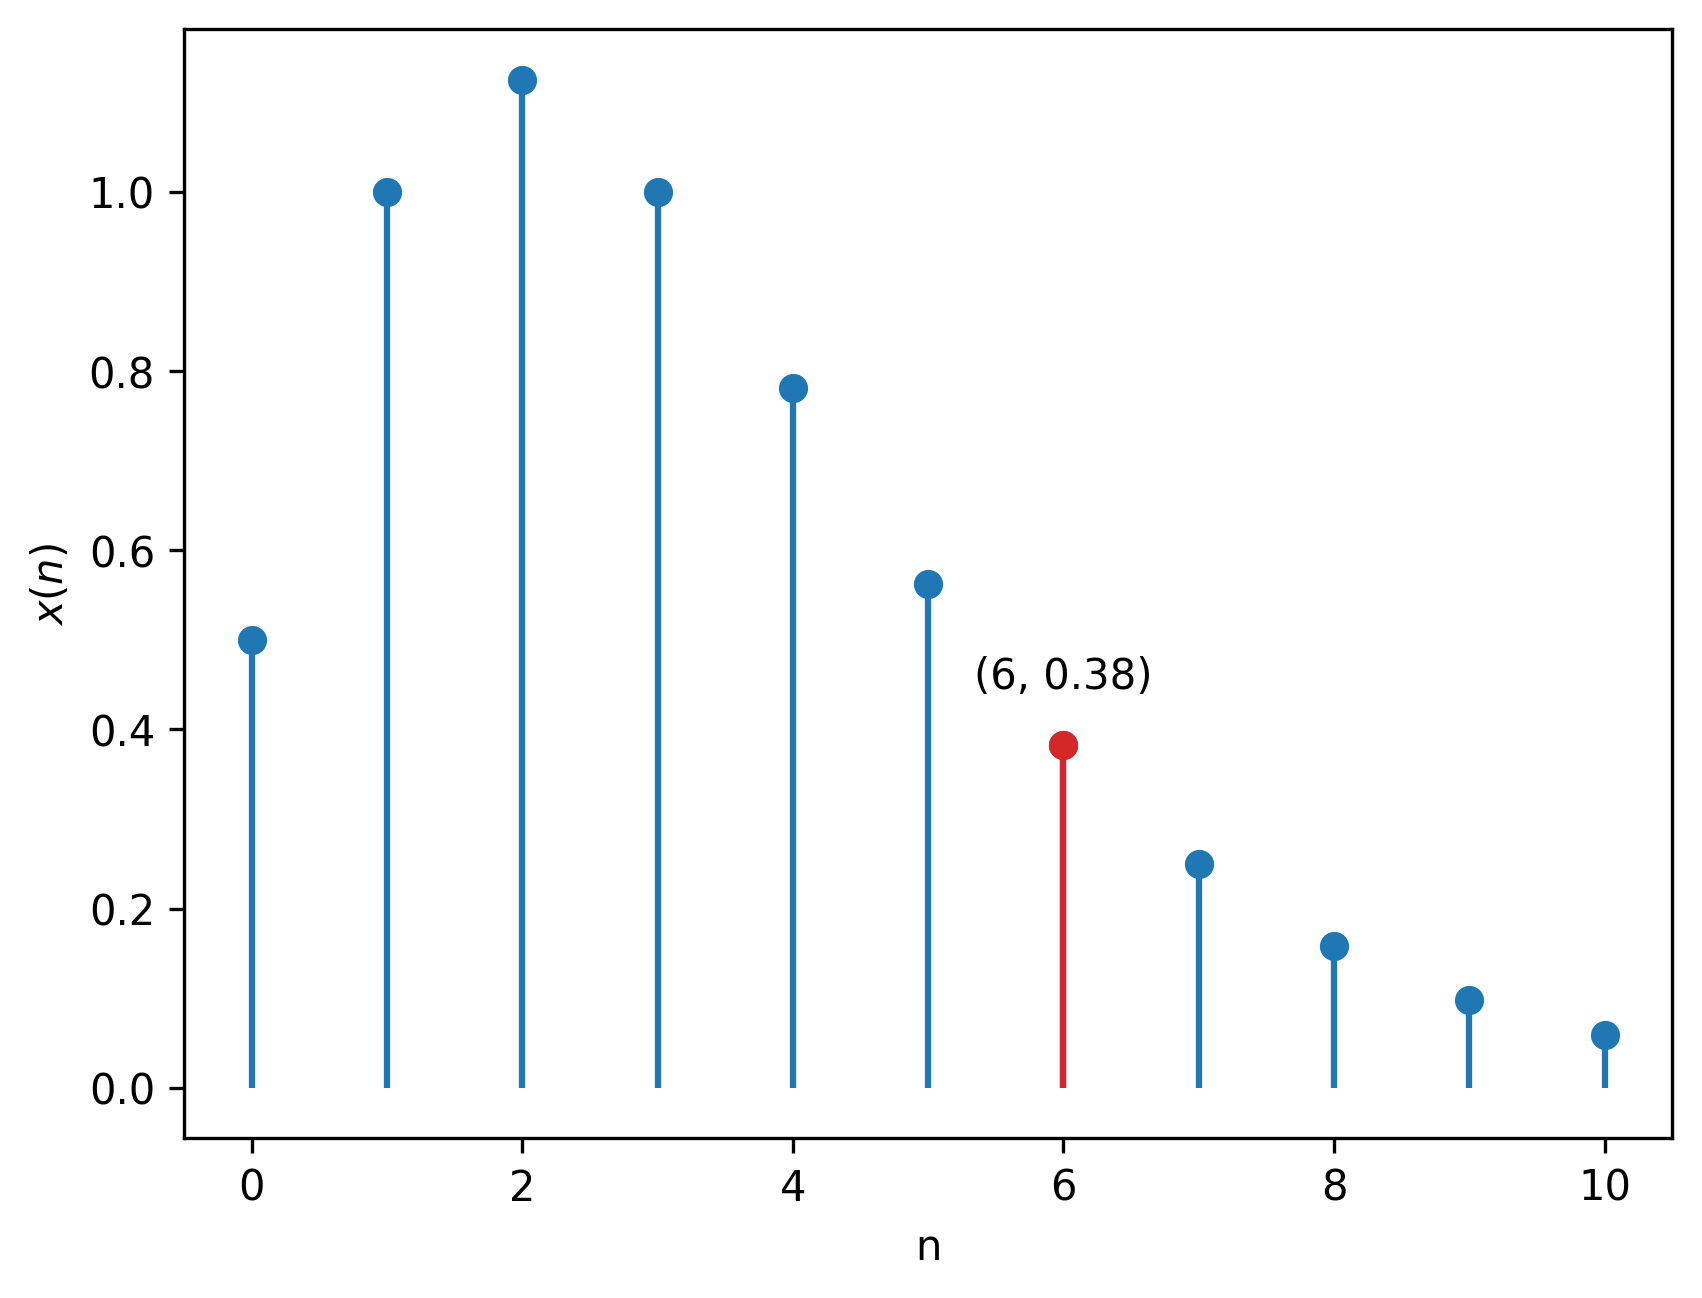
\includegraphics[width=\columnwidth]{ncert-maths/11/9/1/11.9.1.8/figs/plot.png}
    \caption{Stem plot of $x(n)$}
    \label{fig:1}
\end{figure}

%\end{document}

\pagebreak
\item Given below are some functions of x and t to 
represent the displacement (transverse
or longitudinal) of an elastic wave. State which of these represents \brak i travelling
wave, \brak {ii} a stationary wave or \brak {iii} none at all: \\
\begin{enumerate}
\item $y = 2\cos \brak{3x} \sin \brak{10t}$
\item $y=2\sqrt{x-vt}$
\item $y = 3\sin \brak{5x - 0.5t} + 4\cos \brak{5x - 0.5t}$
\item $y = \cos x \sin t + \cos 2x \sin 2t$
\end{enumerate}
\solution
\iffalse
\let\negmedspace\undefined
\let\negthickspace\undefined
\documentclass[journal,12pt,twocolumn]{IEEEtran}
\usepackage{cite}
\usepackage{amsmath,amssymb,amsfonts,amsthm}
\usepackage{algorithmic}
\usepackage{graphicx}
\usepackage{textcomp}
\usepackage{xcolor}
\usepackage{txfonts}
\usepackage{listings}
\usepackage{enumitem}
\usepackage{mathtools}
\usepackage{gensymb}
\usepackage{comment}
\usepackage[breaklinks=true]{hyperref}
\usepackage{tkz-euclide} 
\usepackage{listings}
\usepackage{gvv}                                        
\def\inputGnumericTable{}                                 
\usepackage[latin1]{inputenc}                                
\usepackage{color}                                            
\usepackage{array}                                            
\usepackage{longtable}                                       
\usepackage{calc}                                             
\usepackage{multirow}                                         
\usepackage{hhline}                                           
\usepackage{ifthen}                                           
\usepackage{lscape}
\newtheorem{theorem}{Theorem}[section]
\newtheorem{problem}{Problem}
\newtheorem{proposition}{Proposition}[section]
\newtheorem{lemma}{Lemma}[section]
\newtheorem{corollary}[theorem]{Corollary}
\newtheorem{example}{Example}[section]
\newtheorem{definition}[problem]{Definition}
\newcommand{\BEQA}{\begin{eqnarray}}
\newcommand{\EEQA}{\end{eqnarray}}
\newcommand{\define}{\stackrel{\triangle}{=}}
\theoremstyle{remark}
\newtheorem{rem}{Remark}
\begin{document}
\parindent 0px
\bibliographystyle{IEEEtran}
\title{ASSIGNMENT11.15\_13Q}
\author{EE22BTECH11219 - Sai Sujan Rada$^{}$% <-this % stops a space
}
\maketitle
\newpage
\bigskip
\section*{QUESTION}
Given below are some functions of x and t to 
represent the displacement (transverse
or longitudinal) of an elastic wave. State which of these represents \brak i travelling
wave, \brak {ii} a stationary wave or \brak {iii} none at all: \\
\begin{enumerate}
\item $y = 2\cos \brak{3x} \sin \brak{10t}$
\item $y=2\sqrt{x-vt}$
\item $y = 3\sin \brak{5x - 0.5t} + 4\cos \brak{5x - 0.5t}$
\item $y = \cos x \sin t + \cos 2x \sin 2t$
\end{enumerate}
\solution 
\fi

\input{ncert-physics/11/15/13/tables/TABLE1.tex}
Let us assume an equation:
\begin{align}
y=A(x)\cos \brak{\omega t+\phi\brak {x}}
\end{align}
\input{ncert-physics/11/15/13/tables/TABLE2.tex}
\begin{figure}[h]
                        \centering
                        \includegraphics[width=\columnwidth]{ncert-physics/11/15/13/figs/a.png}
                        \caption{DIPLACEMENT $vs$ TIME-graph1}
                        \label{fig:11.13.1}
\end{figure}
\begin{figure}[h]
                            \centering
                            \includegraphics[width=\columnwidth]{ncert-physics/11/15/13/figs/b.png}
                            \caption{DIPLACEMENT $vs$ TIME-graph2}
                            \label{fig:11.13.2}
\end{figure}   
\begin{figure}[h]
                             \centering
                             \includegraphics[width=\columnwidth]{ncert-physics/11/15/13/figs/c.png}
                             \caption{DIPLACEMENT $vs$ TIME-graph3}
                             \label{fig:11.13.3}
\end{figure}
\begin{figure}[h]
                            \centering
                            \includegraphics[width=\columnwidth]{ncert-physics/11/15/13/figs/d.png}
                            \caption{DIPLACEMENT $vs$ TIME-graph4}
                            \label{fig:11.13.4}
\end{figure}
\figref{fig:11.13.1} and \figref{fig:11.13.3} are self explanatory for stationary and travelling waves.
\figref{fig:11.13.2} and \figref{fig:11.13.4} are neither stationary nor travelling waves. 


\pagebreak
\item For the travelling harmonic wave
$y\brak {x, t} = 2.0 \cos 2\pi \brak{10t - 0.0080 x + 0.35}$ where $x$ and $y$ are in $cm$ and $t$ in $s$. Calculate the phase difference between oscillatory
motion of two points separated by a distance of 

\begin{enumerate} [label=(\alph*)]
    \item $4 m$
    \item $0.5 m$
    \item $\lambda/2$
    \item $3\lambda/4$
\end{enumerate}
\solution
\iffalse
\let\negmedspace\undefined
\let\negthickspace\undefined
\documentclass[journal,12pt,twocolumn]{IEEEtran}
\usepackage{cite}
\usepackage{amsmath,amssymb,amsfonts,amsthm}
\usepackage{algorithmic}
\usepackage{graphicx}
\usepackage{textcomp}
\usepackage{xcolor}
\usepackage{txfonts}
\usepackage{listings}
\usepackage{enumitem}
\usepackage{mathtools}
\usepackage{gensymb}
\usepackage{comment}
\usepackage[breaklinks=true]{hyperref}
\usepackage{tkz-euclide} 
\usepackage{listings}
\usepackage{gvv}                                        
\def\inputGnumericTable{}                                 
\usepackage[latin1]{inputenc}                               \usepackage{caption}
\usepackage{color}                                            
\usepackage{array}                                            
\usepackage{longtable}                                       
\usepackage{calc}                                             
\usepackage{multirow}                                         
\usepackage{hhline}                                           
\usepackage{ifthen}                                           
\usepackage{lscape}

\newtheorem{theorem}{Theorem}[section]
\newtheorem{problem}{Problem}
\newtheorem{proposition}{Proposition}[section]
\newtheorem{lemma}{Lemma}[section]
\newtheorem{corollary}[theorem]{Corollary}
\newtheorem{example}{Example}[section]
\newtheorem{definition}[problem]{Definition}
\newcommand{\BEQA}{\begin{eqnarray}}
\newcommand{\EEQA}{\end{eqnarray}}
\newcommand{\define}{\stackrel{\triangle}{=}}
\theoremstyle{remark}
\newtheorem{rem}{Remark}
\begin{document}

\bibliographystyle{IEEEtran}
\vspace{3cm}

\title{NCERT 11.15. Q10}
\author{EE23BTECH11010 - Venkatesh Bandawar$^{*}$% <-this % stops a space
}
\maketitle
\newpage
\bigskip

\renewcommand{\thefigure}{\arabic{figure}}
\renewcommand{\thetable}{\arabic{table}}

\bibliographystyle{IEEEtran}

\parindent 0px
\textbf{Question:} For the travelling harmonic wave
$y\brak {x, t} = 2.0 \cos 2\pi \brak{10t - 0.0080 x + 0.35}$ where $x$ and $y$ are in $cm$ and $t$ in $s$. Calculate the phase difference between oscillatory
motion of two points separated by a distance of 

\begin{enumerate} [label=(\alph*)]
    \item $4 m$
    \item $0.5 m$
    \item $\lambda/2$
    \item $3\lambda/4$
\end{enumerate}

\solution
\fi
\begin{table}[htbp] \small
\centering
\input{ncert-physics/11/15/10/tables/table1.tex}
\caption{Given \, parameters list}
\label{tab:11.15.10.1}
\end{table}
\begin{align}
    \brak{\Delta \theta} &= \brak{ 2\pi f t - kx_1 + \phi}  - \brak{2\pi f t -kx_2 + \phi}\\
    &= k\brak{x_2 - x_1} 
\end{align}

\begin{table}[htbp] 
\centering
\input{ncert-physics/11/15/10/tables/table2.tex}
\caption{Phase \, differences}
\label{tab:11.15.10.2}
\end{table}

\begin{figure}[!h] 
\centering
\includegraphics[width=\columnwidth]{ncert-physics/11/15/10/figs/graph1.png}
\captionsetup{justification=centering}
\caption{}
\label{fig:11.15.10.1}
\end{figure}

\begin{figure}[!h] 
\centering
\includegraphics[width=\columnwidth]{ncert-physics/11/15/10/figs/graph2.png}
\captionsetup{justification=centering}
\caption{}
\label{fig:11.15.10.2}
\end{figure}

\begin{figure}[!h] 
\centering
\includegraphics[width=\columnwidth]{ncert-physics/11/15/10/figs/graph3.png}
\captionsetup{justification=centering}
\caption{}
\label{fig:11.15.10.3}
\end{figure}

\begin{figure}[!h] 
\centering
\includegraphics[width=\columnwidth]{ncert-physics/11/15/10/figs/graph4.png}
\captionsetup{justification=centering}
\caption{}
\label{fig:11.15.10.4}
\end{figure}


\pagebreak
\item 
\begin{enumerate}
\item The peak voltage of an AC supply is 300 V. What is the rms voltage?
\item The rms value of current in an AC circuit is 10 A. What is the peak current?
\end{enumerate}
\solution
%% Run LaTeX on this file several times to get Table of Contents,
%% cross-references, and citations.
\documentclass[11pt]{book}
\usepackage{gvv-book}
\usepackage{gvv}
%\usepackage{Wiley-AuthoringTemplate}
\usepackage[sectionbib,authoryear]{natbib}% for name-date citation comment the below line
%\usepackage[sectionbib,numbers]{natbib}% for numbered citation comment the above line

%%********************************************************************%%
%%       How many levels of section head would you like numbered?     %%
%% 0= no section numbers, 1= section, 2= subsection, 3= subsubsection %%
\setcounter{secnumdepth}{3}
%%********************************************************************%%
%%**********************************************************************%%
%%     How many levels of section head would you like to appear in the  %%
%%				Table of Contents?			%%
%% 0= chapter, 1= section, 2= subsection, 3= subsubsection titles.	%%
\setcounter{tocdepth}{2}
%%**********************************************************************%%

%\includeonly{ch01}
\makeindex

\begin{document}

\frontmatter
%%%%%%%%%%%%%%%%%%%%%%%%%%%%%%%%%%%%%%%%%%%%%%%%%%%%%%%%%%%%%%%%
%% Title Pages
%% Wiley will provide title and copyright page, but you can make
%% your own titlepages if you'd like anyway
%% Setting up title pages, type in the appropriate names here:

\booktitle{Signal Processing \\ Fundamentals}

\subtitle{Through NCERT}

\AuAff{G. V. V. Sharma}


%% \\ will start a new line.
%% You may add \affil{} for affiliation, ie,
%\authors{Robert M. Groves\\
%\affil{Universitat de les Illes Balears}
%Floyd J. Fowler, Jr.\\
%\affil{University of New Mexico}
%}

%% Print Half Title and Title Page:
%\halftitlepage
\titlepage

%%%%%%%%%%%%%%%%%%%%%%%%%%%%%%%%%%%%%%%%%%%%%%%%%%%%%%%%%%%%%%%%
%% Copyright Page

\begin{copyrightpage}{2024}
%Title, etc
\end{copyrightpage}

% Note, you must use \ to start indented lines, ie,
% 
% \begin{copyrightpage}{2004}
% Survey Methodology / Robert M. Groves . . . [et al.].
% \       p. cm.---(Wiley series in survey methodology)
% \    ``Wiley-Interscience."
% \    Includes bibliographical references and index.
% \    ISBN 0-471-48348-6 (pbk.)
% \    1. Surveys---Methodology.  2. Social 
% \  sciences---Research---Statistical methods.  I. Groves, Robert M.  II. %
% Series.\\

% HA31.2.S873 2004
% 001.4'33---dc22                                             2004044064
% \end{copyrightpage}

%%%%%%%%%%%%%%%%%%%%%%%%%%%%%%%%%%%%%%%%%%%%%%%%%%%%%%%%%%%%%%%%
%% Only Dedication (optional) 

%\dedication{To my parents}

\tableofcontents

%\listoffigures %optional
%\listoftables  %optional

%% or Contributor Page for edited books
%% before \tableofcontents

%%%%%%%%%%%%%%%%%%%%%%%%%%%%%%%%%%%%%%%%%%%%%%%%%%%%%%%%%%%%%%%%
%  Contributors Page for Edited Book
%%%%%%%%%%%%%%%%%%%%%%%%%%%%%%%%%%%%%%%%%%%%%%%%%%%%%%%%%%%%%%%%

% If your book has chapters written by different authors,
% you'll need a Contributors page.

% Use \begin{contributors}...\end{contributors} and
% then enter each author with the \name{} command, followed
% by the affiliation information.

% \begin{contributors}
% \name{Masayki Abe,} Fujitsu Laboratories Ltd., Fujitsu Limited, Atsugi, Japan
%
% \name{L. A. Akers,} Center for Solid State Electronics Research, Arizona State University, Tempe, Arizona
%
% \name{G. H. Bernstein,} Department of Electrical and Computer Engineering, University of Notre Dame, Notre Dame, South Bend, Indiana; formerly of
% Center for Solid State Electronics Research, Arizona
% State University, Tempe, Arizona 
% \end{contributors}

%%%%%%%%%%%%%%%%%%%%%%%%%%%%%%%%%%%%%%%%%%%%%%%%%%%%%%%%%%%%%%%%
% Optional Foreword:

%\begin{foreword}
%\lipsum[1-2]
%\end{foreword}

%%%%%%%%%%%%%%%%%%%%%%%%%%%%%%%%%%%%%%%%%%%%%%%%%%%%%%%%%%%%%%%%
% Optional Preface:

%\begin{preface}
%\lipsum[1-1]
%\prefaceauthor{}
%\where{place\\
% date}
%\end{preface}

% ie,
% \begin{preface}
% This is an example preface.
% \prefaceauthor{R. K. Watts}
% \where{Durham, North Carolina\\
% September, 2004}

%%%%%%%%%%%%%%%%%%%%%%%%%%%%%%%%%%%%%%%%%%%%%%%%%%%%%%%%%%%%%%%%
% Optional Acknowledgments:

%\acknowledgments
%\lipsum[1-2]
%\authorinitials{I. R. S.}  

%%%%%%%%%%%%%%%%%%%%%%%%%%%%%%%%
%% Glossary Type of Environment:

% \begin{glossary}
% \term{<term>}{<description>}
% \end{glossary}

%%%%%%%%%%%%%%%%%%%%%%%%%%%%%%%%
%\begin{acronyms}
%\acro{ASTA}{Arrivals See Time Averages}
%\acro{BHCA}{Busy Hour Call Attempts}
%\acro{BR}{Bandwidth Reservation}
%\acro{b.u.}{bandwidth unit(s)}
%\acro{CAC}{Call / Connection Admission Control}
%\acro{CBP}{Call Blocking Probability(-ies)}
%\acro{CCS}{Centum Call Seconds}
%\acro{CDTM}{Connection Dependent Threshold Model}
%\acro{CS}{Complete Sharing}
%\acro{DiffServ}{Differentiated Services}
%\acro{EMLM}{Erlang Multirate Loss Model}
%\acro{erl}{The Erlang unit of traffic-load}
%\acro{FIFO}{First in - First out}
%\acro{GB}{Global balance}
%\acro{GoS}{Grade of Service}
%\acro{ICT}{Information and Communication Technology}
%\acro{IntServ}{Integrated Services}
%\acro{IP}{Internet Protocol}
%\acro{ITU-T}{International Telecommunication Unit -- Standardization sector}
%\acro{LB}{Local balance}
%\acro{LHS}{Left hand side}
%\acro{LIFO}{Last in - First out}
%\acro{MMPP}{Markov Modulated Poisson Process}
%\acro{MPLS}{Multiple Protocol Labeling Switching}
%\acro{MRM}{Multi-Retry Model}
%\acro{MTM}{Multi-Threshold Model}
%\acro{PASTA}{Poisson Arrivals See Time Averages}
%\acro{PDF}{Probability Distribution Function}
%\acro{pdf}{probability density function}
%\acro{PFS}{Product Form Solution}
%\acro{QoS}{Quality of Service}
%\acro{r.v.}{random variable(s)}
%\acro{RED}{random early detection}
%\acro{RHS}{Right hand side}
%\acro{RLA}{Reduced Load Approximation}
%\acro{SIRO}{service in random order}
%\acro{SRM}{Single-Retry Model}
%\acro{STM}{Single-Threshold Model}
%\acro{TCP}{Transport Control Protocol}
%\acro{TH}{Threshold(s)}
%\acro{UDP}{User Datagram Protocol}
%\end{acronyms}

\setcounter{page}{1}

\begin{introduction}
This book introduces some concepts in signal processing through maths and physics problems in
NCERT textbooks.

\end{introduction}

\mainmatter

\chapter{Analog}
\section{Harmonics}
\input{ncert-physics/analog.tex}
\section{Filters}
\input{ncert-physics/analog-filters.tex}
\chapter{Discrete}
\section{ Z-transform}
\input{ncert-maths/z-transform}
\section{Sequences}
\input{ncert-maths/sequences}
\backmatter
\appendix
\chapter{ Convolution}
\input{app/conv.tex}
\chapter{ Z-transform}
\input{app/mgf.tex}
\latexprintindex

\end{document}

 


\pagebreak
\item In Young’s double-slit experiment using monochromatic light of wavelength $\lambda$, the intensity of light at a point on the screen where path difference is $\lambda$, is $K$ units. What is the intensity of light at a
point where path difference is $\lambda$/3?\\

\solution

%% Run LaTeX on this file several times to get Table of Contents,
%% cross-references, and citations.
\documentclass[11pt]{book}
\usepackage{gvv-book}
\usepackage{gvv}
%\usepackage{Wiley-AuthoringTemplate}
\usepackage[sectionbib,authoryear]{natbib}% for name-date citation comment the below line
%\usepackage[sectionbib,numbers]{natbib}% for numbered citation comment the above line

%%********************************************************************%%
%%       How many levels of section head would you like numbered?     %%
%% 0= no section numbers, 1= section, 2= subsection, 3= subsubsection %%
\setcounter{secnumdepth}{3}
%%********************************************************************%%
%%**********************************************************************%%
%%     How many levels of section head would you like to appear in the  %%
%%				Table of Contents?			%%
%% 0= chapter, 1= section, 2= subsection, 3= subsubsection titles.	%%
\setcounter{tocdepth}{2}
%%**********************************************************************%%

%\includeonly{ch01}
\makeindex

\begin{document}

\frontmatter
%%%%%%%%%%%%%%%%%%%%%%%%%%%%%%%%%%%%%%%%%%%%%%%%%%%%%%%%%%%%%%%%
%% Title Pages
%% Wiley will provide title and copyright page, but you can make
%% your own titlepages if you'd like anyway
%% Setting up title pages, type in the appropriate names here:

\booktitle{Signal Processing \\ Fundamentals}

\subtitle{Through NCERT}

\AuAff{G. V. V. Sharma}


%% \\ will start a new line.
%% You may add \affil{} for affiliation, ie,
%\authors{Robert M. Groves\\
%\affil{Universitat de les Illes Balears}
%Floyd J. Fowler, Jr.\\
%\affil{University of New Mexico}
%}

%% Print Half Title and Title Page:
%\halftitlepage
\titlepage

%%%%%%%%%%%%%%%%%%%%%%%%%%%%%%%%%%%%%%%%%%%%%%%%%%%%%%%%%%%%%%%%
%% Copyright Page

\begin{copyrightpage}{2024}
%Title, etc
\end{copyrightpage}

% Note, you must use \ to start indented lines, ie,
% 
% \begin{copyrightpage}{2004}
% Survey Methodology / Robert M. Groves . . . [et al.].
% \       p. cm.---(Wiley series in survey methodology)
% \    ``Wiley-Interscience."
% \    Includes bibliographical references and index.
% \    ISBN 0-471-48348-6 (pbk.)
% \    1. Surveys---Methodology.  2. Social 
% \  sciences---Research---Statistical methods.  I. Groves, Robert M.  II. %
% Series.\\

% HA31.2.S873 2004
% 001.4'33---dc22                                             2004044064
% \end{copyrightpage}

%%%%%%%%%%%%%%%%%%%%%%%%%%%%%%%%%%%%%%%%%%%%%%%%%%%%%%%%%%%%%%%%
%% Only Dedication (optional) 

%\dedication{To my parents}

\tableofcontents

%\listoffigures %optional
%\listoftables  %optional

%% or Contributor Page for edited books
%% before \tableofcontents

%%%%%%%%%%%%%%%%%%%%%%%%%%%%%%%%%%%%%%%%%%%%%%%%%%%%%%%%%%%%%%%%
%  Contributors Page for Edited Book
%%%%%%%%%%%%%%%%%%%%%%%%%%%%%%%%%%%%%%%%%%%%%%%%%%%%%%%%%%%%%%%%

% If your book has chapters written by different authors,
% you'll need a Contributors page.

% Use \begin{contributors}...\end{contributors} and
% then enter each author with the \name{} command, followed
% by the affiliation information.

% \begin{contributors}
% \name{Masayki Abe,} Fujitsu Laboratories Ltd., Fujitsu Limited, Atsugi, Japan
%
% \name{L. A. Akers,} Center for Solid State Electronics Research, Arizona State University, Tempe, Arizona
%
% \name{G. H. Bernstein,} Department of Electrical and Computer Engineering, University of Notre Dame, Notre Dame, South Bend, Indiana; formerly of
% Center for Solid State Electronics Research, Arizona
% State University, Tempe, Arizona 
% \end{contributors}

%%%%%%%%%%%%%%%%%%%%%%%%%%%%%%%%%%%%%%%%%%%%%%%%%%%%%%%%%%%%%%%%
% Optional Foreword:

%\begin{foreword}
%\lipsum[1-2]
%\end{foreword}

%%%%%%%%%%%%%%%%%%%%%%%%%%%%%%%%%%%%%%%%%%%%%%%%%%%%%%%%%%%%%%%%
% Optional Preface:

%\begin{preface}
%\lipsum[1-1]
%\prefaceauthor{}
%\where{place\\
% date}
%\end{preface}

% ie,
% \begin{preface}
% This is an example preface.
% \prefaceauthor{R. K. Watts}
% \where{Durham, North Carolina\\
% September, 2004}

%%%%%%%%%%%%%%%%%%%%%%%%%%%%%%%%%%%%%%%%%%%%%%%%%%%%%%%%%%%%%%%%
% Optional Acknowledgments:

%\acknowledgments
%\lipsum[1-2]
%\authorinitials{I. R. S.}  

%%%%%%%%%%%%%%%%%%%%%%%%%%%%%%%%
%% Glossary Type of Environment:

% \begin{glossary}
% \term{<term>}{<description>}
% \end{glossary}

%%%%%%%%%%%%%%%%%%%%%%%%%%%%%%%%
%\begin{acronyms}
%\acro{ASTA}{Arrivals See Time Averages}
%\acro{BHCA}{Busy Hour Call Attempts}
%\acro{BR}{Bandwidth Reservation}
%\acro{b.u.}{bandwidth unit(s)}
%\acro{CAC}{Call / Connection Admission Control}
%\acro{CBP}{Call Blocking Probability(-ies)}
%\acro{CCS}{Centum Call Seconds}
%\acro{CDTM}{Connection Dependent Threshold Model}
%\acro{CS}{Complete Sharing}
%\acro{DiffServ}{Differentiated Services}
%\acro{EMLM}{Erlang Multirate Loss Model}
%\acro{erl}{The Erlang unit of traffic-load}
%\acro{FIFO}{First in - First out}
%\acro{GB}{Global balance}
%\acro{GoS}{Grade of Service}
%\acro{ICT}{Information and Communication Technology}
%\acro{IntServ}{Integrated Services}
%\acro{IP}{Internet Protocol}
%\acro{ITU-T}{International Telecommunication Unit -- Standardization sector}
%\acro{LB}{Local balance}
%\acro{LHS}{Left hand side}
%\acro{LIFO}{Last in - First out}
%\acro{MMPP}{Markov Modulated Poisson Process}
%\acro{MPLS}{Multiple Protocol Labeling Switching}
%\acro{MRM}{Multi-Retry Model}
%\acro{MTM}{Multi-Threshold Model}
%\acro{PASTA}{Poisson Arrivals See Time Averages}
%\acro{PDF}{Probability Distribution Function}
%\acro{pdf}{probability density function}
%\acro{PFS}{Product Form Solution}
%\acro{QoS}{Quality of Service}
%\acro{r.v.}{random variable(s)}
%\acro{RED}{random early detection}
%\acro{RHS}{Right hand side}
%\acro{RLA}{Reduced Load Approximation}
%\acro{SIRO}{service in random order}
%\acro{SRM}{Single-Retry Model}
%\acro{STM}{Single-Threshold Model}
%\acro{TCP}{Transport Control Protocol}
%\acro{TH}{Threshold(s)}
%\acro{UDP}{User Datagram Protocol}
%\end{acronyms}

\setcounter{page}{1}

\begin{introduction}
This book introduces some concepts in signal processing through maths and physics problems in
NCERT textbooks.

\end{introduction}

\mainmatter

\chapter{Analog}
\section{Harmonics}
\input{ncert-physics/analog.tex}
\section{Filters}
\input{ncert-physics/analog-filters.tex}
\chapter{Discrete}
\section{ Z-transform}
\input{ncert-maths/z-transform}
\section{Sequences}
\input{ncert-maths/sequences}
\backmatter
\appendix
\chapter{ Convolution}
\input{app/conv.tex}
\chapter{ Z-transform}
\input{app/mgf.tex}
\latexprintindex

\end{document}

 

\pagebreak

\item In a plane electromagnetic wave, the electric field oscillates sinusoidally at a frequency of $2.0 \text{ x } 10^{10}$ Hz and amplitude 48 $Vm^{-1}$.
\begin{enumerate}[label=(\alph*)]
    \item What is the wavelength of the wave?
    \item What is the amplitude of the oscillating magnetic field?
    \item Show that the average energy density of the $\vec{E}$ field equals the
average energy density of the $\vec{B}$ field. $[c = 3 \text{ x } 10^{8}ms^{-1} ]$
\end{enumerate}

\item \begin{enumerate}
\item For the wave on the string $y(x, t) = 0.06 \sin(\frac{2\pi x}{3}) \cos(120\pi t)$ , do all the points on the string     oscillate with the same (a)frequency , (b)phase , (c)amplitude ? Explain your answers. \\

 \item What is the amplitude of a point 0.375m away from one end? \\
 \end{enumerate}
 \solution
 \pagebreak
 
 \item 
 A transverse harmonic wave on a string is described by
\begin{align}
    y\brak{x,t}=3.0 \sin\brak{36t+0.018x+\frac{\pi}{4}}
\end{align}
where $x$ and $y$ are in cm and $t$ in s. The positive direction of $x$ is from left to right.
\begin{enumerate}[label=(\alph*)]
    \item Is this a travelling wave or a stationary wave? If it is travelling, what are the speed and direction of its propogation?
    \item What are its amplitude and frequency?
    \item What is the initial phase at the origin?
    \item  What is the least distance between two succesive crests in the wave?
\end{enumerate}

\solution
\pagebreak

\item In deriving the single slit diffraction pattern, it was stated that the intensity is zero at angles of $\frac{n\lambda}{a}$. Justify this by suitably dividing the slit to bring out the cancellation.\\
\solution
\pagebreak

\item A 60 $\mu$ F capacitor is connected to a 110 V, 60 Hz ac supply. Determine the rms value of the current in the circuit.\\
\solution
\pagebreak

\item A charged  $30\mu F$ capacitor is connected to a $27 mH$ inductor. What is the angular frequency of free oscillations of the circuit?\\
\solution
\pagebreak
\item Obtain the resonance frequency of a series LCR circuit with $L = 2.0\, H$, $C = 32\, \mu F$, and $R = 10\, \Omega$. What is the Q-value of the circuit.\\
\solution
\pagebreak
\item A charged 30 $\mu$F capacitor is connected to a 27 mH inductor. Suppose the initial charge on the capacitor is 6mC.What is the total energy stored in the circuit initially? What is the
total energy at later time? \\
\solution
\pagebreak

\item A wire stretched between two rigid supports vibrates in its fundamental mode with a frequency of $45 \, \text{Hz}$. The mass of the wire is $3.5 \times 10^{-2} \, \text{kg}$, and its linear mass density is $4.0 \times 10^{-2} \, \text{kg/m}$. The length of the wire is $0.875 \, \text{m}$. Determine the speed of a transverse wave on the string and the tension in the string.\\
\solution
\pagebreak

\item The given figure shows a series LCR circuit connected to a variable
frequency 230 V source. \\
L = 5.0 H, C = 80 $\mu$F, R = 40 $\Omega$.

\begin{figure}[h!]
\begin{center}
\begin{circuitikz}[american voltages]
      \draw (0,0)
      to[sV, l=$\varepsilon$] (0,2) 
      to[R, l=$R$, v=$V_R$] (4,2) 
      to[C, l=$C$, v=$V_C$] (4,0)
      to[L, l=$L$, v=$V_L$] (0,0);
\end{circuitikz}
\end{center}
\end{figure}

\begin{enumerate}
    \item Determine the source frequency which drives the circuit in resonance.
    \item Obtain the impedance of the circuit and the amplitude of current
at the resonating frequency.
    \item Determine the rms potential drops across the three elements of
the circuit. Show that the potential drop across the LC
combination is zero at the resonating frequency.\\
\end{enumerate}
\solution
\pagebreak

\item Q23) A narrow sound pulse (for example, a short pip by a whistle) is sent across a
	medium.\\ \brak{\text{a}} Does the pulse have a definite \brak{\text{i}} frequency, \brak{\text{ii}} wavelength, \brak{\text{iii}} speed
	of propagation?\\[1ex]\brak{\text{b}} If the pulse rate is 1 after every 20 s, (that is the whistle is
	blown for a split of second after every 20 s), Is the frequency of note produced
	by whistle equal to 1/20 or 0.05 Hz ?\\
\solution
\pagebreak
\item Suppose that the electric field part of an electromagnetic wave in vacuum given as\\ \textbf{E} =\{(3.1N/C)cos[(1.8 rad/m)y+(5.4$\times$10$^{6}$rad/s)t]\}\^i \\
(a) What is the direction of propagation ?\\
(b) What is the wavelength ? \\
(c) What is the frequency ?\\
(d) What is the amplitude of the magnetic field part of the wave?\\
(e) Write an expression for the magnetic field part of the wave.\\
\solution
\pagebreak

\item A 44 mH inductor is connected to 220 V, 50 Hz ac supply. Determine
the rms value of the current in the circuit.\\
\solution
\pagebreak

\item The 6563 \AA\, H$\alpha$ line emitted by hydrogen in a star is found to be redshifted by 15 \AA. Estimate the speed with which the star is receding from the Earth.
\solution
\pagebreak
\item The amplitude  of the magnetic part of a harmonic elctromagnetic wave is $B_0=510$nT.What is the amplitude of the electric part of the electromagnetic wave.\\
\solution
\pagebreak

\item A 100$\mu$F capacitor in series with a 40$\Omega$ resistance is connected to a 110V, 60Hz supply.
\begin{enumerate}[label = {\brak{\alph*}}]
\item What is the maximum current in the circuit?
\item What is the time lag between the current maximum and the voltage maximum?\\
\end{enumerate}
\solution
\pagebreak
\item A 100 $\ohm$ resistor is connected to $220 V$, $50 Hz$ AC supply.\\
(1) What is the rms value of current in the circuit?\\
(2) What is the net power consumed over a full cycle?

\solution
\pagebreak
\item  Two towers on top of two hills are $40$ km apart.This line joining them passes $50$ m above a hill halfway between the towers.What is the longest wavelength of radio waves,which can be sent between the towers without  appereciable diffraction effects?\\
\solution
\pagebreak
\item A circuit containing a 80mH inductor and a 60$\mu$F capacitor in series is connected to a 230V, 50Hz supply. The resistance of the circuit is negligible.\\
\begin{enumerate}
  \item Obtain the current amplitude and rms value.
  \item Obtain the rms value of potential drops across each element.
  \item What is the average power transferred to the inductor ?
  \item What is the average power transferred to the capacitor ?
  \item What is the total average power absorbed by the circuit ? \brak{\text{'Average' implies 'averaged over one cycle'.}}
\end{enumerate}
\solution
\pagebreak
\item A coil of inductance 0.50 H and resistance 100 $\Omega$ is connected to a 240 V, 50 Hz ac supply.\\
(a) What is the maximum current in the coil?\\		
(b) What is the time lag between the voltage maximum and the current maximum?\\
\solution
\pagebreak

\item A plane electromagnetic wave travels in vacuum along the \(z\)-direction. What can you say about the directions of its electric (\(\mathbf{E}\)) and magnetic (\(\mathbf{B}\)) field vectors? If the frequency of the wave is \(30 \, \text{MHz}\), what can you say about its wavelength?\\
\solution
\pagebreak

\item
Earthquakes generate sound waves inside the earth. Unlike a gas, the earth can experience both transverse (S) and longitudinal (P) sound waves. Typically the speed of S wave is about $4.0 km/s$, and that of P wave is $8.0 km/s$. A seismograph records P and S waves from an earthquake. The first P wave arrives $4 min$ before the first S wave. Assuming the waves travel in straight line, at what distance does the
earthquake occur ?
\solution
\pagebreak

\item
A hospital uses an ultrasonic scanner to locate tumors in a tissue. What is the wavelength of sound in the tissue in which the speed of sound is $1.7 \, \text{km/s}$? The operating frequency of the scanner is $4.2 \, \text{MHz}$.
\solution
\pagebreak

\item In double-slit experiment using light of wavelength $600 nm$, the
angular width of a fringe formed on a distant screen is $0.1\degree$. What is
the spacing between the two slits?\\
\solution
\pagebreak

\item Figures correspond to two circular motions. The radius of the circle, the period of revolution, the initial position and the sense of revolution(i.e. clockwise or anti-clockwise) are indicated on each figure. Obtain the corresponding simple harmonic motions of the x-projections of the radius vector of resolving particle P in each case.

\begin{figure}[h]
        \centering
        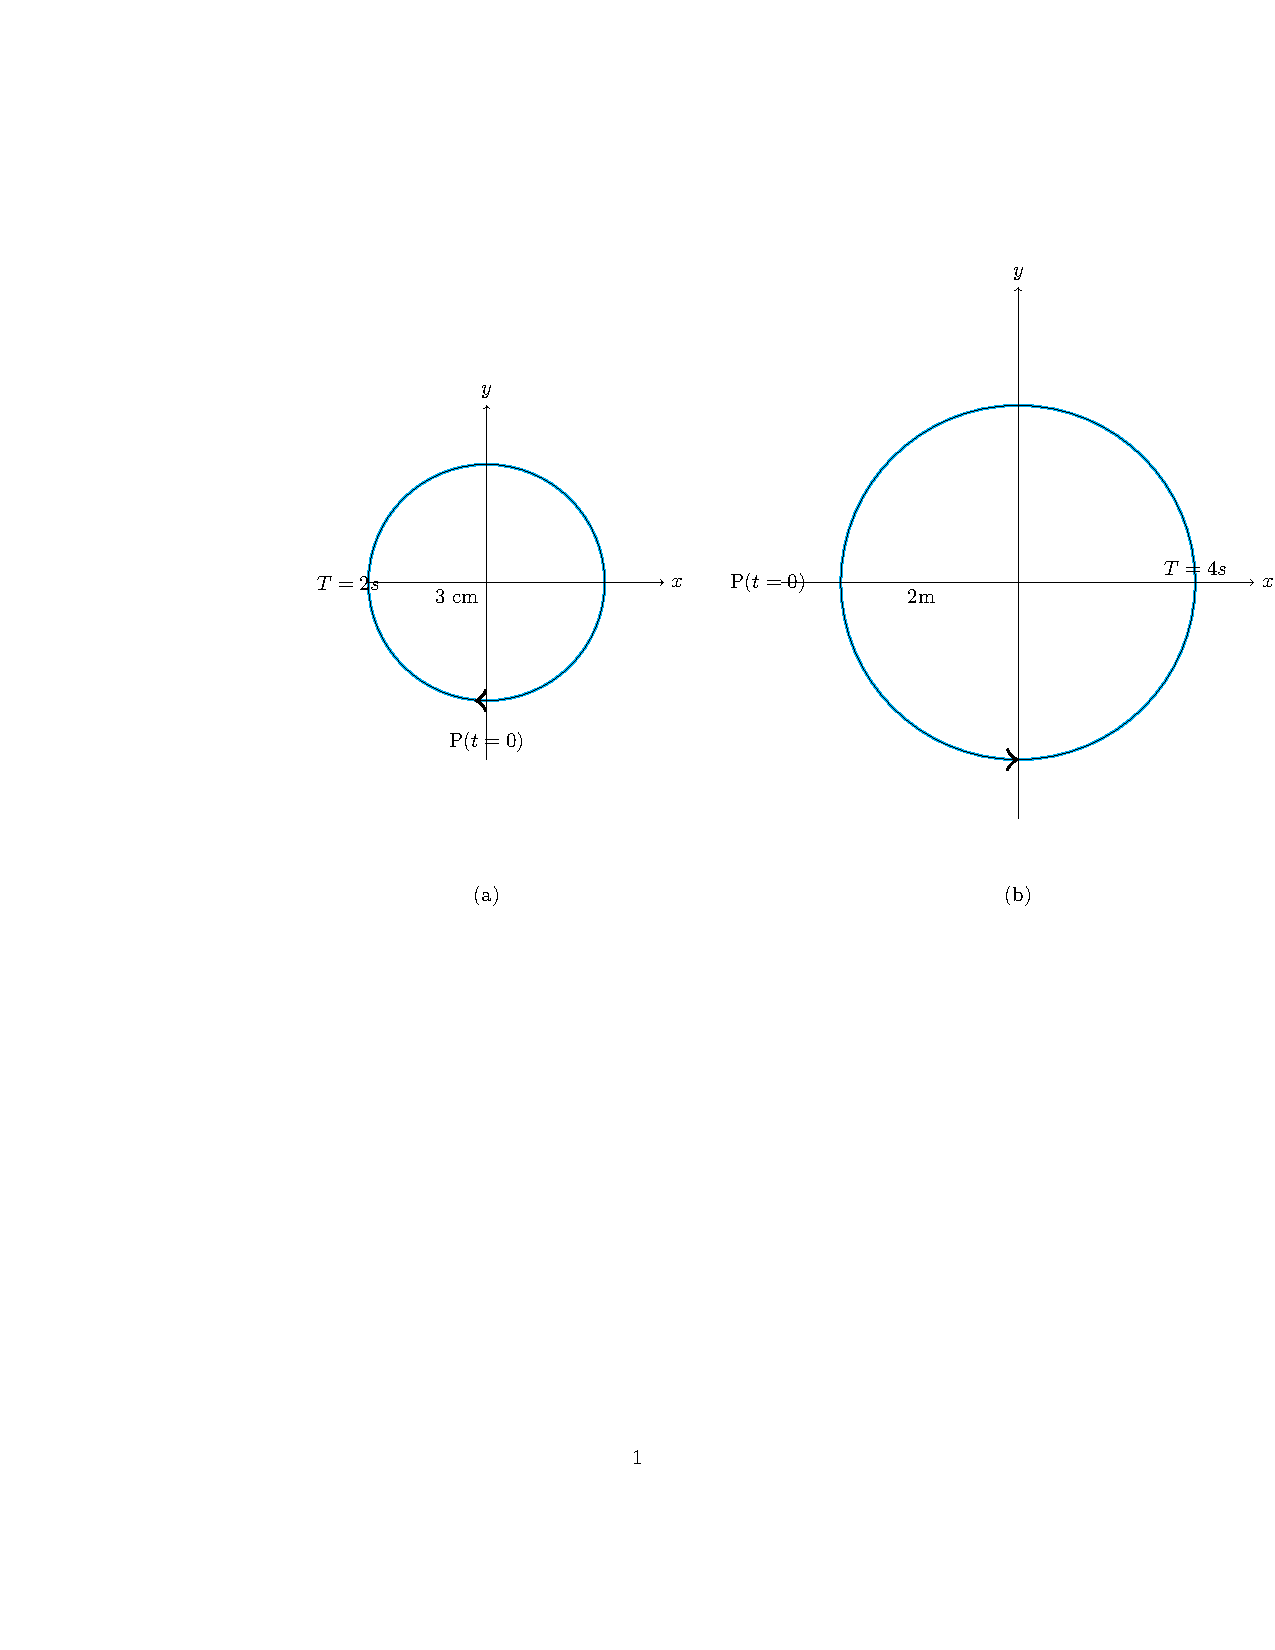
\includegraphics[width=0.5\columnwidth]{ncert-physics/11/14/11/codes/qfig.pdf}
\end{figure}
\solution
\pagebreak



\end{enumerate}

\section{Filters}
\begin{enumerate}[label=\thesection.\arabic*,ref=\thesection.\theenumi]
\item An LC circuit contains a $50 \mu H$ inductor and a $50 \mu F$ capacitor with an initial charge of $10 mC$. The resistance of the circuit is negligible. Let the instant the circuit is closed by $t = 0$.

\textbf{a)} What is the total energy stored initially? Is it conserved during LC oscillations?

\textbf{b)} What is the natural frequency of the circuit?

\textbf{c)} At what time is the energy stored \textbf{(i)} completely electrical (i.e., stored in the capacitor)? \textbf{(ii)} completely magnetic (i.e., stored in the inductor)?

\textbf{d)} At what times is the total energy shared equally between the inductor and the capacitor?

\textbf{e)} If a resistor is inserted in the circuit, how much energy is eventually dissipated as heat? \\
\hfill(NCERT-Physics 12.7 12Q)\\
\solution 
\pagebreak 

\item Obtain the resonant frequency and Q-factor of a series LCR circuit with $L = 3.0\, H$, $C = 27\, \mu F$, and $R = 7.4\, \Omega$. It is desired to improve the sharpness of the resonance of the circuit by reducing its `full width at half maximum' by a factor of 2. Suggest a suitable way.\\
\solution
\input{ncert-physics/12/7/21/Phy_12_7_21.tex}

\pagebreak
\item A circuit containing a $80 mH$ inductor and a $60 \mu F$ capacitor in series is connected to a $230 V$, $50 Hz$ supply. A resistance of $15 \Omega $ is connected in series. Obtain the average power transferred to each element of the circuit, and the total power absorbed.\\
\solution
\pagebreak

\item A series LCR circuit with 
$L$ = $0.12 H$
$C$ = $480 nF$
$R$ = $23 \Omega$
is connected to a $230 V$ variable frequency supply.\\
(a) What is the source frequency for which current amplitude is maximum? Obtain this maximum value.\\
(b) What is the source frequency for which the average power absorbed by the circuit is maximum? Obtain the value of this maximum power.\\
(c) For which frequencies of the source is the power transferred to the circuit half the power at resonant frequency? What is the current amplitude at these frequencies?\\
(d) What is the Q-factor of the given circuit?\\
\solution
\pagebreak

\item A 100$\mu$F capacitor in series with a 40$\Omega$ resistance is connected to a 110 V, 12 kHz supply.
\begin{enumerate}[label=\alph*)]
	\item What is the maximum current in the circuit?
	\item What is the time lag between the current maximum and the voltage maximum?
\end{enumerate}
Hence, explain the statement that a capacitor is a conductor at very high frequencies. Compare this behaviour with that ofa a capacitor in a dc circuit after the steady state.\\
\solution
\pagebreak

\end{enumerate}

\chapter{Discrete}
\section{ Z-transform}
\begin{enumerate}[label=\thesection.\arabic*,ref=\thesection.\theenumi]
\item The $4^{th}$ term of a G.P. is square of its second term, and the first term is -3. Determine its $7^{th}$ term.\\  

\solution 

\iffalse
\let\negmedspace\undefined
\let\negthickspace\undefined
\documentclass[journal,12pt,twocolumn]{IEEEtran}
\usepackage{cite}
\usepackage{amsmath,amssymb,amsfonts,amsthm}
\usepackage{algorithmic}
\usepackage{graphicx}
\usepackage{textcomp}
\usepackage{xcolor}
\usepackage{txfonts}
\usepackage{listings}
\usepackage{enumitem}
\usepackage{mathtools}
\usepackage{gensymb}
\usepackage{comment}
\usepackage[breaklinks=true]{hyperref}
\usepackage{tkz-euclide}
\usepackage{listings}
\usepackage{gvv}
\def\inputGnumericTable{}
\usepackage[latin1]{inputenc}
\usepackage{color}
\usepackage{array}
\usepackage{longtable}
\usepackage{calc}
\usepackage{multirow}
\usepackage{hhline}
\usepackage{ifthen}
\usepackage{lscape}

\newtheorem{theorem}{Theorem}[section]
\newtheorem{problem}{Problem}
\newtheorem{proposition}{Proposition}[section]
\newtheorem{lemma}{Lemma}[section]
\newtheorem{corollary}[theorem]{Corollary}
\newtheorem{example}{Example}[section]
\newtheorem{definition}[problem]{Definition}
\newcommand{\BEQA}{\begin{eqnarray}}
\newcommand{\EEQA}{\end{eqnarray}}
\newcommand{\define}{\stackrel{\triangle}{=}}
\theoremstyle{remark}
\newtheorem{rem}{Remark}
\begin{document}

\bibliographystyle{IEEEtran}
\vspace{3cm}

\title{NCERT Discrete - 10.5.3.20}
\author{EE23BTECH1205 - Avani Chouhan$^{*}$% <-this % stops a space
}
\maketitle
\newpage
\bigskip

\renewcommand{\thefigure}{\theenumi}
\renewcommand{\thetable}{\theenumi}

\vspace{3cm}
\textbf{Question : 10.5.3.20} 
The sum of some terms of G.P. is 315 whose first term and the common ratio are $5$ and $2$ , respectively. Find the last term and the number of terms.\\
\solution
\fi
\begin{table}
  \centering
  \input{ncert-maths/11/9/5/8/tables/table2.tex}
  \caption{Input Parameters}
  \label{tab:10.5.3.20table1}
\end{table}
\begin{align}
x(n) = x(0)r^{n}u(n)
\label{eq:10.5.3.20eq}
\end{align}
From \eqref{eq:gpz}
\begin{align}
X(z) =\frac{5}{1-2z^{-1}} \quad \abs{z} > \abs{2}
\end{align}
By contour integration:
\begin{align}
y(n) &= x(0)\brak{\frac{r^{n+1}-1}{r-1}}u(n)\\
315 &= 5\brak{2^{n+1}- 1}  \\
\implies n &= 5
\end{align}
The number of terms is \(n + 1 = 6\)\\
From \eqref{eq:10.5.3.20eq}:
\begin{align}
x(5) &= 5\brak{2^{5}}\\
 &= 160 
\end{align}

\begin{figure}[H]
    \centering
    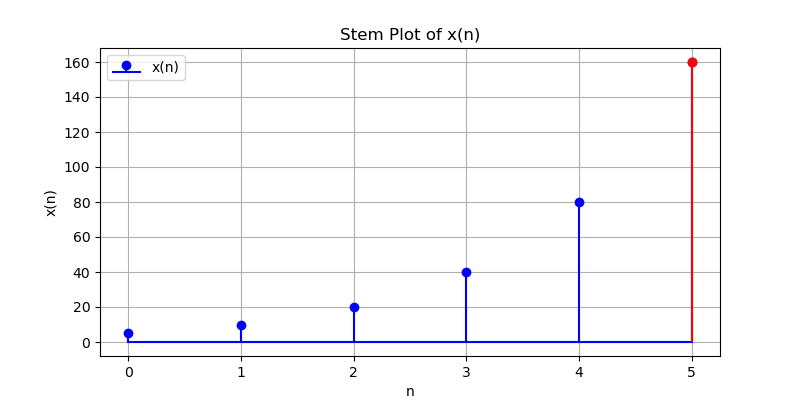
\includegraphics[width=\columnwidth]{ncert-maths/11/9/5/8/figs/plot1.png}
    \caption{Stem plot of x(n)}
    \label{fig:10.5.3.20fig1}
\end{figure}
\begin{figure}[H]
    \centering
    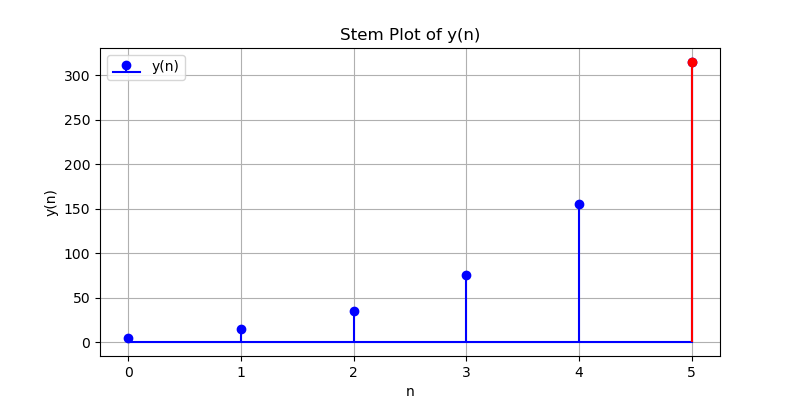
\includegraphics[width=\columnwidth]{ncert-maths/11/9/5/8/figs/plot2.png}
    \caption{Stem plot of y(n)}
    \label{fig:10.5.3.20fig2}
\end{figure}
%\end{document}

\pagebreak

\item Show that
\begin{equation}
    \frac{1\times2^2 + 2\times3^2 + \dots + n\times\brak{n+1}^2}{1^2\times2 + 2^2\times3 +\dots + n^2\times\brak{n+1}}  = \frac{3n+5}{3n+1}\notag
\end{equation}

\solution 

%% Run LaTeX on this file several times to get Table of Contents,
%% cross-references, and citations.
\documentclass[11pt]{book}
\usepackage{gvv-book}
\usepackage{gvv}
%\usepackage{Wiley-AuthoringTemplate}
\usepackage[sectionbib,authoryear]{natbib}% for name-date citation comment the below line
%\usepackage[sectionbib,numbers]{natbib}% for numbered citation comment the above line

%%********************************************************************%%
%%       How many levels of section head would you like numbered?     %%
%% 0= no section numbers, 1= section, 2= subsection, 3= subsubsection %%
\setcounter{secnumdepth}{3}
%%********************************************************************%%
%%**********************************************************************%%
%%     How many levels of section head would you like to appear in the  %%
%%				Table of Contents?			%%
%% 0= chapter, 1= section, 2= subsection, 3= subsubsection titles.	%%
\setcounter{tocdepth}{2}
%%**********************************************************************%%

%\includeonly{ch01}
\makeindex

\begin{document}

\frontmatter
%%%%%%%%%%%%%%%%%%%%%%%%%%%%%%%%%%%%%%%%%%%%%%%%%%%%%%%%%%%%%%%%
%% Title Pages
%% Wiley will provide title and copyright page, but you can make
%% your own titlepages if you'd like anyway
%% Setting up title pages, type in the appropriate names here:

\booktitle{Signal Processing \\ Fundamentals}

\subtitle{Through NCERT}

\AuAff{G. V. V. Sharma}


%% \\ will start a new line.
%% You may add \affil{} for affiliation, ie,
%\authors{Robert M. Groves\\
%\affil{Universitat de les Illes Balears}
%Floyd J. Fowler, Jr.\\
%\affil{University of New Mexico}
%}

%% Print Half Title and Title Page:
%\halftitlepage
\titlepage

%%%%%%%%%%%%%%%%%%%%%%%%%%%%%%%%%%%%%%%%%%%%%%%%%%%%%%%%%%%%%%%%
%% Copyright Page

\begin{copyrightpage}{2024}
%Title, etc
\end{copyrightpage}

% Note, you must use \ to start indented lines, ie,
% 
% \begin{copyrightpage}{2004}
% Survey Methodology / Robert M. Groves . . . [et al.].
% \       p. cm.---(Wiley series in survey methodology)
% \    ``Wiley-Interscience."
% \    Includes bibliographical references and index.
% \    ISBN 0-471-48348-6 (pbk.)
% \    1. Surveys---Methodology.  2. Social 
% \  sciences---Research---Statistical methods.  I. Groves, Robert M.  II. %
% Series.\\

% HA31.2.S873 2004
% 001.4'33---dc22                                             2004044064
% \end{copyrightpage}

%%%%%%%%%%%%%%%%%%%%%%%%%%%%%%%%%%%%%%%%%%%%%%%%%%%%%%%%%%%%%%%%
%% Only Dedication (optional) 

%\dedication{To my parents}

\tableofcontents

%\listoffigures %optional
%\listoftables  %optional

%% or Contributor Page for edited books
%% before \tableofcontents

%%%%%%%%%%%%%%%%%%%%%%%%%%%%%%%%%%%%%%%%%%%%%%%%%%%%%%%%%%%%%%%%
%  Contributors Page for Edited Book
%%%%%%%%%%%%%%%%%%%%%%%%%%%%%%%%%%%%%%%%%%%%%%%%%%%%%%%%%%%%%%%%

% If your book has chapters written by different authors,
% you'll need a Contributors page.

% Use \begin{contributors}...\end{contributors} and
% then enter each author with the \name{} command, followed
% by the affiliation information.

% \begin{contributors}
% \name{Masayki Abe,} Fujitsu Laboratories Ltd., Fujitsu Limited, Atsugi, Japan
%
% \name{L. A. Akers,} Center for Solid State Electronics Research, Arizona State University, Tempe, Arizona
%
% \name{G. H. Bernstein,} Department of Electrical and Computer Engineering, University of Notre Dame, Notre Dame, South Bend, Indiana; formerly of
% Center for Solid State Electronics Research, Arizona
% State University, Tempe, Arizona 
% \end{contributors}

%%%%%%%%%%%%%%%%%%%%%%%%%%%%%%%%%%%%%%%%%%%%%%%%%%%%%%%%%%%%%%%%
% Optional Foreword:

%\begin{foreword}
%\lipsum[1-2]
%\end{foreword}

%%%%%%%%%%%%%%%%%%%%%%%%%%%%%%%%%%%%%%%%%%%%%%%%%%%%%%%%%%%%%%%%
% Optional Preface:

%\begin{preface}
%\lipsum[1-1]
%\prefaceauthor{}
%\where{place\\
% date}
%\end{preface}

% ie,
% \begin{preface}
% This is an example preface.
% \prefaceauthor{R. K. Watts}
% \where{Durham, North Carolina\\
% September, 2004}

%%%%%%%%%%%%%%%%%%%%%%%%%%%%%%%%%%%%%%%%%%%%%%%%%%%%%%%%%%%%%%%%
% Optional Acknowledgments:

%\acknowledgments
%\lipsum[1-2]
%\authorinitials{I. R. S.}  

%%%%%%%%%%%%%%%%%%%%%%%%%%%%%%%%
%% Glossary Type of Environment:

% \begin{glossary}
% \term{<term>}{<description>}
% \end{glossary}

%%%%%%%%%%%%%%%%%%%%%%%%%%%%%%%%
%\begin{acronyms}
%\acro{ASTA}{Arrivals See Time Averages}
%\acro{BHCA}{Busy Hour Call Attempts}
%\acro{BR}{Bandwidth Reservation}
%\acro{b.u.}{bandwidth unit(s)}
%\acro{CAC}{Call / Connection Admission Control}
%\acro{CBP}{Call Blocking Probability(-ies)}
%\acro{CCS}{Centum Call Seconds}
%\acro{CDTM}{Connection Dependent Threshold Model}
%\acro{CS}{Complete Sharing}
%\acro{DiffServ}{Differentiated Services}
%\acro{EMLM}{Erlang Multirate Loss Model}
%\acro{erl}{The Erlang unit of traffic-load}
%\acro{FIFO}{First in - First out}
%\acro{GB}{Global balance}
%\acro{GoS}{Grade of Service}
%\acro{ICT}{Information and Communication Technology}
%\acro{IntServ}{Integrated Services}
%\acro{IP}{Internet Protocol}
%\acro{ITU-T}{International Telecommunication Unit -- Standardization sector}
%\acro{LB}{Local balance}
%\acro{LHS}{Left hand side}
%\acro{LIFO}{Last in - First out}
%\acro{MMPP}{Markov Modulated Poisson Process}
%\acro{MPLS}{Multiple Protocol Labeling Switching}
%\acro{MRM}{Multi-Retry Model}
%\acro{MTM}{Multi-Threshold Model}
%\acro{PASTA}{Poisson Arrivals See Time Averages}
%\acro{PDF}{Probability Distribution Function}
%\acro{pdf}{probability density function}
%\acro{PFS}{Product Form Solution}
%\acro{QoS}{Quality of Service}
%\acro{r.v.}{random variable(s)}
%\acro{RED}{random early detection}
%\acro{RHS}{Right hand side}
%\acro{RLA}{Reduced Load Approximation}
%\acro{SIRO}{service in random order}
%\acro{SRM}{Single-Retry Model}
%\acro{STM}{Single-Threshold Model}
%\acro{TCP}{Transport Control Protocol}
%\acro{TH}{Threshold(s)}
%\acro{UDP}{User Datagram Protocol}
%\end{acronyms}

\setcounter{page}{1}

\begin{introduction}
This book introduces some concepts in signal processing through maths and physics problems in
NCERT textbooks.

\end{introduction}

\mainmatter

\chapter{Analog}
\section{Harmonics}
\input{ncert-physics/analog.tex}
\section{Filters}
\input{ncert-physics/analog-filters.tex}
\chapter{Discrete}
\section{ Z-transform}
\input{ncert-maths/z-transform}
\section{Sequences}
\input{ncert-maths/sequences}
\backmatter
\appendix
\chapter{ Convolution}
\input{app/conv.tex}
\chapter{ Z-transform}
\input{app/mgf.tex}
\latexprintindex

\end{document}

 

\pagebreak

\item Write the five terms at n = 1, 2, 3, 4, 5 of the sequence and obtain the Z-transform of the series
\begin{align}
    x \brak{n} &=  -1, & n = 0 \\
    &=   \frac{x \brak{n-1}}{n}, & n > 0\\
    &=   0, & n < 0 
\end{align}

\solution

%% Run LaTeX on this file several times to get Table of Contents,
%% cross-references, and citations.
\documentclass[11pt]{book}
\usepackage{gvv-book}
\usepackage{gvv}
%\usepackage{Wiley-AuthoringTemplate}
\usepackage[sectionbib,authoryear]{natbib}% for name-date citation comment the below line
%\usepackage[sectionbib,numbers]{natbib}% for numbered citation comment the above line

%%********************************************************************%%
%%       How many levels of section head would you like numbered?     %%
%% 0= no section numbers, 1= section, 2= subsection, 3= subsubsection %%
\setcounter{secnumdepth}{3}
%%********************************************************************%%
%%**********************************************************************%%
%%     How many levels of section head would you like to appear in the  %%
%%				Table of Contents?			%%
%% 0= chapter, 1= section, 2= subsection, 3= subsubsection titles.	%%
\setcounter{tocdepth}{2}
%%**********************************************************************%%

%\includeonly{ch01}
\makeindex

\begin{document}

\frontmatter
%%%%%%%%%%%%%%%%%%%%%%%%%%%%%%%%%%%%%%%%%%%%%%%%%%%%%%%%%%%%%%%%
%% Title Pages
%% Wiley will provide title and copyright page, but you can make
%% your own titlepages if you'd like anyway
%% Setting up title pages, type in the appropriate names here:

\booktitle{Signal Processing \\ Fundamentals}

\subtitle{Through NCERT}

\AuAff{G. V. V. Sharma}


%% \\ will start a new line.
%% You may add \affil{} for affiliation, ie,
%\authors{Robert M. Groves\\
%\affil{Universitat de les Illes Balears}
%Floyd J. Fowler, Jr.\\
%\affil{University of New Mexico}
%}

%% Print Half Title and Title Page:
%\halftitlepage
\titlepage

%%%%%%%%%%%%%%%%%%%%%%%%%%%%%%%%%%%%%%%%%%%%%%%%%%%%%%%%%%%%%%%%
%% Copyright Page

\begin{copyrightpage}{2024}
%Title, etc
\end{copyrightpage}

% Note, you must use \ to start indented lines, ie,
% 
% \begin{copyrightpage}{2004}
% Survey Methodology / Robert M. Groves . . . [et al.].
% \       p. cm.---(Wiley series in survey methodology)
% \    ``Wiley-Interscience."
% \    Includes bibliographical references and index.
% \    ISBN 0-471-48348-6 (pbk.)
% \    1. Surveys---Methodology.  2. Social 
% \  sciences---Research---Statistical methods.  I. Groves, Robert M.  II. %
% Series.\\

% HA31.2.S873 2004
% 001.4'33---dc22                                             2004044064
% \end{copyrightpage}

%%%%%%%%%%%%%%%%%%%%%%%%%%%%%%%%%%%%%%%%%%%%%%%%%%%%%%%%%%%%%%%%
%% Only Dedication (optional) 

%\dedication{To my parents}

\tableofcontents

%\listoffigures %optional
%\listoftables  %optional

%% or Contributor Page for edited books
%% before \tableofcontents

%%%%%%%%%%%%%%%%%%%%%%%%%%%%%%%%%%%%%%%%%%%%%%%%%%%%%%%%%%%%%%%%
%  Contributors Page for Edited Book
%%%%%%%%%%%%%%%%%%%%%%%%%%%%%%%%%%%%%%%%%%%%%%%%%%%%%%%%%%%%%%%%

% If your book has chapters written by different authors,
% you'll need a Contributors page.

% Use \begin{contributors}...\end{contributors} and
% then enter each author with the \name{} command, followed
% by the affiliation information.

% \begin{contributors}
% \name{Masayki Abe,} Fujitsu Laboratories Ltd., Fujitsu Limited, Atsugi, Japan
%
% \name{L. A. Akers,} Center for Solid State Electronics Research, Arizona State University, Tempe, Arizona
%
% \name{G. H. Bernstein,} Department of Electrical and Computer Engineering, University of Notre Dame, Notre Dame, South Bend, Indiana; formerly of
% Center for Solid State Electronics Research, Arizona
% State University, Tempe, Arizona 
% \end{contributors}

%%%%%%%%%%%%%%%%%%%%%%%%%%%%%%%%%%%%%%%%%%%%%%%%%%%%%%%%%%%%%%%%
% Optional Foreword:

%\begin{foreword}
%\lipsum[1-2]
%\end{foreword}

%%%%%%%%%%%%%%%%%%%%%%%%%%%%%%%%%%%%%%%%%%%%%%%%%%%%%%%%%%%%%%%%
% Optional Preface:

%\begin{preface}
%\lipsum[1-1]
%\prefaceauthor{}
%\where{place\\
% date}
%\end{preface}

% ie,
% \begin{preface}
% This is an example preface.
% \prefaceauthor{R. K. Watts}
% \where{Durham, North Carolina\\
% September, 2004}

%%%%%%%%%%%%%%%%%%%%%%%%%%%%%%%%%%%%%%%%%%%%%%%%%%%%%%%%%%%%%%%%
% Optional Acknowledgments:

%\acknowledgments
%\lipsum[1-2]
%\authorinitials{I. R. S.}  

%%%%%%%%%%%%%%%%%%%%%%%%%%%%%%%%
%% Glossary Type of Environment:

% \begin{glossary}
% \term{<term>}{<description>}
% \end{glossary}

%%%%%%%%%%%%%%%%%%%%%%%%%%%%%%%%
%\begin{acronyms}
%\acro{ASTA}{Arrivals See Time Averages}
%\acro{BHCA}{Busy Hour Call Attempts}
%\acro{BR}{Bandwidth Reservation}
%\acro{b.u.}{bandwidth unit(s)}
%\acro{CAC}{Call / Connection Admission Control}
%\acro{CBP}{Call Blocking Probability(-ies)}
%\acro{CCS}{Centum Call Seconds}
%\acro{CDTM}{Connection Dependent Threshold Model}
%\acro{CS}{Complete Sharing}
%\acro{DiffServ}{Differentiated Services}
%\acro{EMLM}{Erlang Multirate Loss Model}
%\acro{erl}{The Erlang unit of traffic-load}
%\acro{FIFO}{First in - First out}
%\acro{GB}{Global balance}
%\acro{GoS}{Grade of Service}
%\acro{ICT}{Information and Communication Technology}
%\acro{IntServ}{Integrated Services}
%\acro{IP}{Internet Protocol}
%\acro{ITU-T}{International Telecommunication Unit -- Standardization sector}
%\acro{LB}{Local balance}
%\acro{LHS}{Left hand side}
%\acro{LIFO}{Last in - First out}
%\acro{MMPP}{Markov Modulated Poisson Process}
%\acro{MPLS}{Multiple Protocol Labeling Switching}
%\acro{MRM}{Multi-Retry Model}
%\acro{MTM}{Multi-Threshold Model}
%\acro{PASTA}{Poisson Arrivals See Time Averages}
%\acro{PDF}{Probability Distribution Function}
%\acro{pdf}{probability density function}
%\acro{PFS}{Product Form Solution}
%\acro{QoS}{Quality of Service}
%\acro{r.v.}{random variable(s)}
%\acro{RED}{random early detection}
%\acro{RHS}{Right hand side}
%\acro{RLA}{Reduced Load Approximation}
%\acro{SIRO}{service in random order}
%\acro{SRM}{Single-Retry Model}
%\acro{STM}{Single-Threshold Model}
%\acro{TCP}{Transport Control Protocol}
%\acro{TH}{Threshold(s)}
%\acro{UDP}{User Datagram Protocol}
%\end{acronyms}

\setcounter{page}{1}

\begin{introduction}
This book introduces some concepts in signal processing through maths and physics problems in
NCERT textbooks.

\end{introduction}

\mainmatter

\chapter{Analog}
\section{Harmonics}
\input{ncert-physics/analog.tex}
\section{Filters}
\input{ncert-physics/analog-filters.tex}
\chapter{Discrete}
\section{ Z-transform}
\input{ncert-maths/z-transform}
\section{Sequences}
\input{ncert-maths/sequences}
\backmatter
\appendix
\chapter{ Convolution}
\input{app/conv.tex}
\chapter{ Z-transform}
\input{app/mgf.tex}
\latexprintindex

\end{document}

 

\pagebreak


\item Subba Rao started work in 1995 at an annual salary of Rs. 5000 and received an increment of Rs. 200 each year. In which year did his income reach Rs. 7000?

\solution

%% Run LaTeX on this file several times to get Table of Contents,
%% cross-references, and citations.
\documentclass[11pt]{book}
\usepackage{gvv-book}
\usepackage{gvv}
%\usepackage{Wiley-AuthoringTemplate}
\usepackage[sectionbib,authoryear]{natbib}% for name-date citation comment the below line
%\usepackage[sectionbib,numbers]{natbib}% for numbered citation comment the above line

%%********************************************************************%%
%%       How many levels of section head would you like numbered?     %%
%% 0= no section numbers, 1= section, 2= subsection, 3= subsubsection %%
\setcounter{secnumdepth}{3}
%%********************************************************************%%
%%**********************************************************************%%
%%     How many levels of section head would you like to appear in the  %%
%%				Table of Contents?			%%
%% 0= chapter, 1= section, 2= subsection, 3= subsubsection titles.	%%
\setcounter{tocdepth}{2}
%%**********************************************************************%%

%\includeonly{ch01}
\makeindex

\begin{document}

\frontmatter
%%%%%%%%%%%%%%%%%%%%%%%%%%%%%%%%%%%%%%%%%%%%%%%%%%%%%%%%%%%%%%%%
%% Title Pages
%% Wiley will provide title and copyright page, but you can make
%% your own titlepages if you'd like anyway
%% Setting up title pages, type in the appropriate names here:

\booktitle{Signal Processing \\ Fundamentals}

\subtitle{Through NCERT}

\AuAff{G. V. V. Sharma}


%% \\ will start a new line.
%% You may add \affil{} for affiliation, ie,
%\authors{Robert M. Groves\\
%\affil{Universitat de les Illes Balears}
%Floyd J. Fowler, Jr.\\
%\affil{University of New Mexico}
%}

%% Print Half Title and Title Page:
%\halftitlepage
\titlepage

%%%%%%%%%%%%%%%%%%%%%%%%%%%%%%%%%%%%%%%%%%%%%%%%%%%%%%%%%%%%%%%%
%% Copyright Page

\begin{copyrightpage}{2024}
%Title, etc
\end{copyrightpage}

% Note, you must use \ to start indented lines, ie,
% 
% \begin{copyrightpage}{2004}
% Survey Methodology / Robert M. Groves . . . [et al.].
% \       p. cm.---(Wiley series in survey methodology)
% \    ``Wiley-Interscience."
% \    Includes bibliographical references and index.
% \    ISBN 0-471-48348-6 (pbk.)
% \    1. Surveys---Methodology.  2. Social 
% \  sciences---Research---Statistical methods.  I. Groves, Robert M.  II. %
% Series.\\

% HA31.2.S873 2004
% 001.4'33---dc22                                             2004044064
% \end{copyrightpage}

%%%%%%%%%%%%%%%%%%%%%%%%%%%%%%%%%%%%%%%%%%%%%%%%%%%%%%%%%%%%%%%%
%% Only Dedication (optional) 

%\dedication{To my parents}

\tableofcontents

%\listoffigures %optional
%\listoftables  %optional

%% or Contributor Page for edited books
%% before \tableofcontents

%%%%%%%%%%%%%%%%%%%%%%%%%%%%%%%%%%%%%%%%%%%%%%%%%%%%%%%%%%%%%%%%
%  Contributors Page for Edited Book
%%%%%%%%%%%%%%%%%%%%%%%%%%%%%%%%%%%%%%%%%%%%%%%%%%%%%%%%%%%%%%%%

% If your book has chapters written by different authors,
% you'll need a Contributors page.

% Use \begin{contributors}...\end{contributors} and
% then enter each author with the \name{} command, followed
% by the affiliation information.

% \begin{contributors}
% \name{Masayki Abe,} Fujitsu Laboratories Ltd., Fujitsu Limited, Atsugi, Japan
%
% \name{L. A. Akers,} Center for Solid State Electronics Research, Arizona State University, Tempe, Arizona
%
% \name{G. H. Bernstein,} Department of Electrical and Computer Engineering, University of Notre Dame, Notre Dame, South Bend, Indiana; formerly of
% Center for Solid State Electronics Research, Arizona
% State University, Tempe, Arizona 
% \end{contributors}

%%%%%%%%%%%%%%%%%%%%%%%%%%%%%%%%%%%%%%%%%%%%%%%%%%%%%%%%%%%%%%%%
% Optional Foreword:

%\begin{foreword}
%\lipsum[1-2]
%\end{foreword}

%%%%%%%%%%%%%%%%%%%%%%%%%%%%%%%%%%%%%%%%%%%%%%%%%%%%%%%%%%%%%%%%
% Optional Preface:

%\begin{preface}
%\lipsum[1-1]
%\prefaceauthor{}
%\where{place\\
% date}
%\end{preface}

% ie,
% \begin{preface}
% This is an example preface.
% \prefaceauthor{R. K. Watts}
% \where{Durham, North Carolina\\
% September, 2004}

%%%%%%%%%%%%%%%%%%%%%%%%%%%%%%%%%%%%%%%%%%%%%%%%%%%%%%%%%%%%%%%%
% Optional Acknowledgments:

%\acknowledgments
%\lipsum[1-2]
%\authorinitials{I. R. S.}  

%%%%%%%%%%%%%%%%%%%%%%%%%%%%%%%%
%% Glossary Type of Environment:

% \begin{glossary}
% \term{<term>}{<description>}
% \end{glossary}

%%%%%%%%%%%%%%%%%%%%%%%%%%%%%%%%
%\begin{acronyms}
%\acro{ASTA}{Arrivals See Time Averages}
%\acro{BHCA}{Busy Hour Call Attempts}
%\acro{BR}{Bandwidth Reservation}
%\acro{b.u.}{bandwidth unit(s)}
%\acro{CAC}{Call / Connection Admission Control}
%\acro{CBP}{Call Blocking Probability(-ies)}
%\acro{CCS}{Centum Call Seconds}
%\acro{CDTM}{Connection Dependent Threshold Model}
%\acro{CS}{Complete Sharing}
%\acro{DiffServ}{Differentiated Services}
%\acro{EMLM}{Erlang Multirate Loss Model}
%\acro{erl}{The Erlang unit of traffic-load}
%\acro{FIFO}{First in - First out}
%\acro{GB}{Global balance}
%\acro{GoS}{Grade of Service}
%\acro{ICT}{Information and Communication Technology}
%\acro{IntServ}{Integrated Services}
%\acro{IP}{Internet Protocol}
%\acro{ITU-T}{International Telecommunication Unit -- Standardization sector}
%\acro{LB}{Local balance}
%\acro{LHS}{Left hand side}
%\acro{LIFO}{Last in - First out}
%\acro{MMPP}{Markov Modulated Poisson Process}
%\acro{MPLS}{Multiple Protocol Labeling Switching}
%\acro{MRM}{Multi-Retry Model}
%\acro{MTM}{Multi-Threshold Model}
%\acro{PASTA}{Poisson Arrivals See Time Averages}
%\acro{PDF}{Probability Distribution Function}
%\acro{pdf}{probability density function}
%\acro{PFS}{Product Form Solution}
%\acro{QoS}{Quality of Service}
%\acro{r.v.}{random variable(s)}
%\acro{RED}{random early detection}
%\acro{RHS}{Right hand side}
%\acro{RLA}{Reduced Load Approximation}
%\acro{SIRO}{service in random order}
%\acro{SRM}{Single-Retry Model}
%\acro{STM}{Single-Threshold Model}
%\acro{TCP}{Transport Control Protocol}
%\acro{TH}{Threshold(s)}
%\acro{UDP}{User Datagram Protocol}
%\end{acronyms}

\setcounter{page}{1}

\begin{introduction}
This book introduces some concepts in signal processing through maths and physics problems in
NCERT textbooks.

\end{introduction}

\mainmatter

\chapter{Analog}
\section{Harmonics}
\input{ncert-physics/analog.tex}
\section{Filters}
\input{ncert-physics/analog-filters.tex}
\chapter{Discrete}
\section{ Z-transform}
\input{ncert-maths/z-transform}
\section{Sequences}
\input{ncert-maths/sequences}
\backmatter
\appendix
\chapter{ Convolution}
\input{app/conv.tex}
\chapter{ Z-transform}
\input{app/mgf.tex}
\latexprintindex

\end{document}

 


\item Consider the sequence whose $n^\text{th}$ term is given by \(2^n\). Find the first 6 terms of this sequence.

\solution

\iffalse
\documentclass[12pt]{article}
\usepackage{amsmath , amssymb}
\usepackage{graphicx}
\usepackage{float}
\usepackage{pgfplots}
\pgfplotsset{compat=1.18}
\newcommand{\tabref}[1]{Table~\ref{#1}}
\newcommand{\figref}[1]{Figure~\ref{#1}}
\providecommand{\abs}[1]{\left\vert#1\right\vert}

\begin{document}

\title{Discrete Assignment}
\author{Mohana Eppala\\ EE23BTECH11018}
\maketitle

\section*{Problem Statement}
Find the value of $n$ so that $\frac{a^{n+1} + b^{n+1}}{a^{n}+b^{n}}$ may be the geometric mean between $a$ and $b$.
\section*{Solution}
\fi
\begin{table}[H]
\input{ncert-maths/11/9/3/27/tables/tab2.tex}
\end{table}

Consider a GP as in \tabref{tab:1},
\begin{align}
	\therefore \frac{a^{n+1} + b^{n+1}}{a^{n}+b^{n}} &= x(1) \\
	\implies a^{n+1} + b^{n+1} &= a^{n+\frac{1}{2}}b^{\frac{1}{2}} + a^{\frac{1}{2}}b^{n+\frac{1}{2}} \\
\implies a^{n+\frac{1}{2}}(a^{\frac{1}{2}} - b^{\frac{1}{2}}) &= b^{n+\frac{1}{2}}(a^{\frac{1}{2}} - b^{\frac{1}{2}}) \\
\implies (\frac{a}{b})^{n+\frac{1}{2}} &= (\frac{a}{b})^{0} \\
\implies n &= -\frac{1}{2}
\end{align}
From \tabref{tab:1},
\begin{align}
	X(z) &= \frac{a}{1-(\sqrt{\frac{b}{a}})z^{-1}} \quad \abs{z}>\abs{\sqrt{\frac{b}{a}}}
\end{align}
%\end{document}


\item If the sum of first 7 terms of an AP is 49 and that of 17 terms is 289, find the sum of first n terms.

\solution

\iffalse
\let\negmedspace\undefined
\let\negthickspace\undefined
\documentclass[journal,12pt,twocolumn]{IEEEtran}
\usepackage{cite}
\usepackage{amsmath,amssymb,amsfonts,amsthm}
\usepackage{algorithmic}
\usepackage{graphicx}
\usepackage{textcomp}
\usepackage{xcolor}
\usepackage{txfonts}
\usepackage{listings}
\usepackage{enumitem}
\usepackage{mathtools}
\usepackage{gensymb}
\usepackage{comment}
\usepackage[breaklinks=true]{hyperref}
\usepackage{tkz-euclide} 
\usepackage{listings}
\usepackage{gvv}                                        
\def\inputGnumericTable{}                                 
\usepackage[latin1]{inputenc}                                
\usepackage{color}                                            
\usepackage{array}                                            
\usepackage{longtable}                                       
\usepackage{calc}                                             
\usepackage{multirow}                                         
\usepackage{hhline}                                           
\usepackage{ifthen}                                           
\usepackage{lscape}
\newtheorem{theorem}{Theorem}[section]
\newtheorem{problem}{Problem}
\newtheorem{proposition}{Proposition}[section]
\newtheorem{lemma}{Lemma}[section]
\newtheorem{corollary}[theorem]{Corollary}
\newtheorem{example}{Example}[section]
\newtheorem{definition}[problem]{Definition}
\newcommand{\BEQA}{\begin{eqnarray}}
\newcommand{\EEQA}{\end{eqnarray}}
\newcommand{\define}{\stackrel{\triangle}{=}}
\theoremstyle{remark}
\newtheorem{rem}{Remark}
\begin{document}

\bibliographystyle{IEEEtran}
\vspace{3cm}

\title{10.5.3.9}
\author{EE23BTECH11063 - Vemula Siddhartha
}
\maketitle
\newpage
\bigskip

\renewcommand{\thefigure}{\theenumi}
\renewcommand{\thetable}{\theenumi}
\textbf{Question}:\\
If the sum of first 7 terms of an AP is 49 and that of 17 terms is 289, find the sum of
first n terms.
\\
\textbf{Solution: }
\fi
\begin{table}[h!]    
  \centering
  \input{ncert-maths/10/5/3/9/tables/table.tex}
  \caption{Variables Used}
  \label{tab10.5.3.9.1}
\end{table}
\begin{align}
y\brak{n}&=\frac{n+1}{2}\,\brak{2x\brak{0}+nd}\,u\brak{n}\label{eq10.5.3.9.1}\\
y\brak{6}&=49\\
y\brak{16}&=289
\end{align}
Then,
\begin{align}
x\brak{0}+3d&=7\label{eq10.5.3.9.2}\\
x\brak{0}+8d&=17 \label{eq10.5.3.9.3}
\end{align}
From  equations \ref{eq10.5.3.9.2} and \ref{eq10.5.3.9.3}, the augmented matrix is:
\begin{align}
 \myvec{
   1 & 3 & 7
   \\
   1 & 8 & 17
 }
 \xleftrightarrow[]{R_2 \leftarrow {R_2-R_1}}
 \myvec{
   1 & 3 & 7
   \\
   0 & 5 & 10
 }
 \\
 \xleftrightarrow[]{R_1 \leftarrow {R_1-\frac{3}{5}R_2}}
 \myvec{
   1 & 0 & 1
   \\
   0 & 5 & 10
 }
 \\
 \xleftrightarrow[]{R_2 \leftarrow \frac{R_2}{5}}
 \myvec{
   1 & 0 & 1
   \\
   0 & 1 & 2
 }
 \\
 \implies \myvec{
   x\brak{0}
   \\
   d
 }
 =
 \myvec{
   1
   \\
   2
 }
\end{align}
\begin{align}
    x\brak{n}&= \brak{1+2n}u\brak{n}\\
    X\brak{z}&=\frac{1}{1-z^{-1}}+\frac{2z^{-1}}{\brak{1-z^{-1}}^2}\;\;\cbrak{z\in\mathbb{C}: |z|>1}
\end{align}
\begin{align}
   y\brak{n}&=x\brak{n}*u\brak{n}\\
   Y\brak{z}&=X\brak{z}\,U\brak{z}\\
   \implies Y\brak{z}&=\brak{\frac{1}{1-z^{-1}}+\frac{2z^{-1}}{\brak{1-z^{-1}}^2}}\brak{\frac{1}{1-z^{-1}}}\\
   &=\frac{1}{\brak{1-z^{-1}}^2}+\frac{2z^{-1}}{\brak{1-z^{-1}}^3}\\
   \brak{n+1}u\brak{n}&\system{Z}\frac{1}{\brak{1-z^{-1}}^2}\cbrak{z\in\mathbb{C}: |z|>1}\\
   n\brak{\brak{n+1}u\brak{n}}&\system{Z}\frac{2z^{-1}}{\brak{1-z^{-1}}^3}\cbrak{z\in\mathbb{C}: |z|>1}
\end{align}
   From equations \eqref{eq:uzder-shift} and \eqref{eq:uzder-der}, taking the inverse Z Transform,
   \begin{align}
   y\brak{n}&=\brak{n+1}u\brak{n}+n\brak{\brak{n+1}u\brak{n}}\\
   \implies y\brak{n}&=\brak{n+1}^2\,u\brak{n}
\end{align}
\begin{figure}[h!]
   \centering
   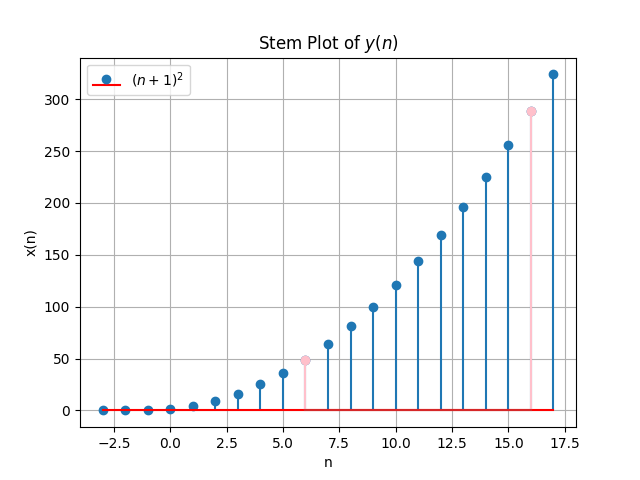
\includegraphics[width=1.1\linewidth]{ncert-maths/10/5/3/9/figs/Figure_1.png}
   \caption{Stem Plot of y\brak{n}}
   \label{stemplot}
\end{figure}

\pagebreak

\item Write the first five terms of the sequence and obtain the corresponding series:\\
$a_1=a_2=2,$ $a_n=a_{n-1} -1,$ $n>2$\\
\solution
%% Run LaTeX on this file several times to get Table of Contents,
%% cross-references, and citations.
\documentclass[11pt]{book}
\usepackage{gvv-book}
\usepackage{gvv}
%\usepackage{Wiley-AuthoringTemplate}
\usepackage[sectionbib,authoryear]{natbib}% for name-date citation comment the below line
%\usepackage[sectionbib,numbers]{natbib}% for numbered citation comment the above line

%%********************************************************************%%
%%       How many levels of section head would you like numbered?     %%
%% 0= no section numbers, 1= section, 2= subsection, 3= subsubsection %%
\setcounter{secnumdepth}{3}
%%********************************************************************%%
%%**********************************************************************%%
%%     How many levels of section head would you like to appear in the  %%
%%				Table of Contents?			%%
%% 0= chapter, 1= section, 2= subsection, 3= subsubsection titles.	%%
\setcounter{tocdepth}{2}
%%**********************************************************************%%

%\includeonly{ch01}
\makeindex

\begin{document}

\frontmatter
%%%%%%%%%%%%%%%%%%%%%%%%%%%%%%%%%%%%%%%%%%%%%%%%%%%%%%%%%%%%%%%%
%% Title Pages
%% Wiley will provide title and copyright page, but you can make
%% your own titlepages if you'd like anyway
%% Setting up title pages, type in the appropriate names here:

\booktitle{Signal Processing \\ Fundamentals}

\subtitle{Through NCERT}

\AuAff{G. V. V. Sharma}


%% \\ will start a new line.
%% You may add \affil{} for affiliation, ie,
%\authors{Robert M. Groves\\
%\affil{Universitat de les Illes Balears}
%Floyd J. Fowler, Jr.\\
%\affil{University of New Mexico}
%}

%% Print Half Title and Title Page:
%\halftitlepage
\titlepage

%%%%%%%%%%%%%%%%%%%%%%%%%%%%%%%%%%%%%%%%%%%%%%%%%%%%%%%%%%%%%%%%
%% Copyright Page

\begin{copyrightpage}{2024}
%Title, etc
\end{copyrightpage}

% Note, you must use \ to start indented lines, ie,
% 
% \begin{copyrightpage}{2004}
% Survey Methodology / Robert M. Groves . . . [et al.].
% \       p. cm.---(Wiley series in survey methodology)
% \    ``Wiley-Interscience."
% \    Includes bibliographical references and index.
% \    ISBN 0-471-48348-6 (pbk.)
% \    1. Surveys---Methodology.  2. Social 
% \  sciences---Research---Statistical methods.  I. Groves, Robert M.  II. %
% Series.\\

% HA31.2.S873 2004
% 001.4'33---dc22                                             2004044064
% \end{copyrightpage}

%%%%%%%%%%%%%%%%%%%%%%%%%%%%%%%%%%%%%%%%%%%%%%%%%%%%%%%%%%%%%%%%
%% Only Dedication (optional) 

%\dedication{To my parents}

\tableofcontents

%\listoffigures %optional
%\listoftables  %optional

%% or Contributor Page for edited books
%% before \tableofcontents

%%%%%%%%%%%%%%%%%%%%%%%%%%%%%%%%%%%%%%%%%%%%%%%%%%%%%%%%%%%%%%%%
%  Contributors Page for Edited Book
%%%%%%%%%%%%%%%%%%%%%%%%%%%%%%%%%%%%%%%%%%%%%%%%%%%%%%%%%%%%%%%%

% If your book has chapters written by different authors,
% you'll need a Contributors page.

% Use \begin{contributors}...\end{contributors} and
% then enter each author with the \name{} command, followed
% by the affiliation information.

% \begin{contributors}
% \name{Masayki Abe,} Fujitsu Laboratories Ltd., Fujitsu Limited, Atsugi, Japan
%
% \name{L. A. Akers,} Center for Solid State Electronics Research, Arizona State University, Tempe, Arizona
%
% \name{G. H. Bernstein,} Department of Electrical and Computer Engineering, University of Notre Dame, Notre Dame, South Bend, Indiana; formerly of
% Center for Solid State Electronics Research, Arizona
% State University, Tempe, Arizona 
% \end{contributors}

%%%%%%%%%%%%%%%%%%%%%%%%%%%%%%%%%%%%%%%%%%%%%%%%%%%%%%%%%%%%%%%%
% Optional Foreword:

%\begin{foreword}
%\lipsum[1-2]
%\end{foreword}

%%%%%%%%%%%%%%%%%%%%%%%%%%%%%%%%%%%%%%%%%%%%%%%%%%%%%%%%%%%%%%%%
% Optional Preface:

%\begin{preface}
%\lipsum[1-1]
%\prefaceauthor{}
%\where{place\\
% date}
%\end{preface}

% ie,
% \begin{preface}
% This is an example preface.
% \prefaceauthor{R. K. Watts}
% \where{Durham, North Carolina\\
% September, 2004}

%%%%%%%%%%%%%%%%%%%%%%%%%%%%%%%%%%%%%%%%%%%%%%%%%%%%%%%%%%%%%%%%
% Optional Acknowledgments:

%\acknowledgments
%\lipsum[1-2]
%\authorinitials{I. R. S.}  

%%%%%%%%%%%%%%%%%%%%%%%%%%%%%%%%
%% Glossary Type of Environment:

% \begin{glossary}
% \term{<term>}{<description>}
% \end{glossary}

%%%%%%%%%%%%%%%%%%%%%%%%%%%%%%%%
%\begin{acronyms}
%\acro{ASTA}{Arrivals See Time Averages}
%\acro{BHCA}{Busy Hour Call Attempts}
%\acro{BR}{Bandwidth Reservation}
%\acro{b.u.}{bandwidth unit(s)}
%\acro{CAC}{Call / Connection Admission Control}
%\acro{CBP}{Call Blocking Probability(-ies)}
%\acro{CCS}{Centum Call Seconds}
%\acro{CDTM}{Connection Dependent Threshold Model}
%\acro{CS}{Complete Sharing}
%\acro{DiffServ}{Differentiated Services}
%\acro{EMLM}{Erlang Multirate Loss Model}
%\acro{erl}{The Erlang unit of traffic-load}
%\acro{FIFO}{First in - First out}
%\acro{GB}{Global balance}
%\acro{GoS}{Grade of Service}
%\acro{ICT}{Information and Communication Technology}
%\acro{IntServ}{Integrated Services}
%\acro{IP}{Internet Protocol}
%\acro{ITU-T}{International Telecommunication Unit -- Standardization sector}
%\acro{LB}{Local balance}
%\acro{LHS}{Left hand side}
%\acro{LIFO}{Last in - First out}
%\acro{MMPP}{Markov Modulated Poisson Process}
%\acro{MPLS}{Multiple Protocol Labeling Switching}
%\acro{MRM}{Multi-Retry Model}
%\acro{MTM}{Multi-Threshold Model}
%\acro{PASTA}{Poisson Arrivals See Time Averages}
%\acro{PDF}{Probability Distribution Function}
%\acro{pdf}{probability density function}
%\acro{PFS}{Product Form Solution}
%\acro{QoS}{Quality of Service}
%\acro{r.v.}{random variable(s)}
%\acro{RED}{random early detection}
%\acro{RHS}{Right hand side}
%\acro{RLA}{Reduced Load Approximation}
%\acro{SIRO}{service in random order}
%\acro{SRM}{Single-Retry Model}
%\acro{STM}{Single-Threshold Model}
%\acro{TCP}{Transport Control Protocol}
%\acro{TH}{Threshold(s)}
%\acro{UDP}{User Datagram Protocol}
%\end{acronyms}

\setcounter{page}{1}

\begin{introduction}
This book introduces some concepts in signal processing through maths and physics problems in
NCERT textbooks.

\end{introduction}

\mainmatter

\chapter{Analog}
\section{Harmonics}
\input{ncert-physics/analog.tex}
\section{Filters}
\input{ncert-physics/analog-filters.tex}
\chapter{Discrete}
\section{ Z-transform}
\input{ncert-maths/z-transform}
\section{Sequences}
\input{ncert-maths/sequences}
\backmatter
\appendix
\chapter{ Convolution}
\input{app/conv.tex}
\chapter{ Z-transform}
\input{app/mgf.tex}
\latexprintindex

\end{document}

 

\pagebreak
\item Insert two numbers between 3 and 81 so that the resulting sequence is G.P.\\

\solution
\input{ncert-maths/11/9/3/26/asnmt1.tex}
\pagebreak

\item  What will Rs 500 amounts to in 10 years after its deposit in a bank which pays annual interest rate of 10$\%$ compounded annually?

\solution
    %% Run LaTeX on this file several times to get Table of Contents,
%% cross-references, and citations.
\documentclass[11pt]{book}
\usepackage{gvv-book}
\usepackage{gvv}
%\usepackage{Wiley-AuthoringTemplate}
\usepackage[sectionbib,authoryear]{natbib}% for name-date citation comment the below line
%\usepackage[sectionbib,numbers]{natbib}% for numbered citation comment the above line

%%********************************************************************%%
%%       How many levels of section head would you like numbered?     %%
%% 0= no section numbers, 1= section, 2= subsection, 3= subsubsection %%
\setcounter{secnumdepth}{3}
%%********************************************************************%%
%%**********************************************************************%%
%%     How many levels of section head would you like to appear in the  %%
%%				Table of Contents?			%%
%% 0= chapter, 1= section, 2= subsection, 3= subsubsection titles.	%%
\setcounter{tocdepth}{2}
%%**********************************************************************%%

%\includeonly{ch01}
\makeindex

\begin{document}

\frontmatter
%%%%%%%%%%%%%%%%%%%%%%%%%%%%%%%%%%%%%%%%%%%%%%%%%%%%%%%%%%%%%%%%
%% Title Pages
%% Wiley will provide title and copyright page, but you can make
%% your own titlepages if you'd like anyway
%% Setting up title pages, type in the appropriate names here:

\booktitle{Signal Processing \\ Fundamentals}

\subtitle{Through NCERT}

\AuAff{G. V. V. Sharma}


%% \\ will start a new line.
%% You may add \affil{} for affiliation, ie,
%\authors{Robert M. Groves\\
%\affil{Universitat de les Illes Balears}
%Floyd J. Fowler, Jr.\\
%\affil{University of New Mexico}
%}

%% Print Half Title and Title Page:
%\halftitlepage
\titlepage

%%%%%%%%%%%%%%%%%%%%%%%%%%%%%%%%%%%%%%%%%%%%%%%%%%%%%%%%%%%%%%%%
%% Copyright Page

\begin{copyrightpage}{2024}
%Title, etc
\end{copyrightpage}

% Note, you must use \ to start indented lines, ie,
% 
% \begin{copyrightpage}{2004}
% Survey Methodology / Robert M. Groves . . . [et al.].
% \       p. cm.---(Wiley series in survey methodology)
% \    ``Wiley-Interscience."
% \    Includes bibliographical references and index.
% \    ISBN 0-471-48348-6 (pbk.)
% \    1. Surveys---Methodology.  2. Social 
% \  sciences---Research---Statistical methods.  I. Groves, Robert M.  II. %
% Series.\\

% HA31.2.S873 2004
% 001.4'33---dc22                                             2004044064
% \end{copyrightpage}

%%%%%%%%%%%%%%%%%%%%%%%%%%%%%%%%%%%%%%%%%%%%%%%%%%%%%%%%%%%%%%%%
%% Only Dedication (optional) 

%\dedication{To my parents}

\tableofcontents

%\listoffigures %optional
%\listoftables  %optional

%% or Contributor Page for edited books
%% before \tableofcontents

%%%%%%%%%%%%%%%%%%%%%%%%%%%%%%%%%%%%%%%%%%%%%%%%%%%%%%%%%%%%%%%%
%  Contributors Page for Edited Book
%%%%%%%%%%%%%%%%%%%%%%%%%%%%%%%%%%%%%%%%%%%%%%%%%%%%%%%%%%%%%%%%

% If your book has chapters written by different authors,
% you'll need a Contributors page.

% Use \begin{contributors}...\end{contributors} and
% then enter each author with the \name{} command, followed
% by the affiliation information.

% \begin{contributors}
% \name{Masayki Abe,} Fujitsu Laboratories Ltd., Fujitsu Limited, Atsugi, Japan
%
% \name{L. A. Akers,} Center for Solid State Electronics Research, Arizona State University, Tempe, Arizona
%
% \name{G. H. Bernstein,} Department of Electrical and Computer Engineering, University of Notre Dame, Notre Dame, South Bend, Indiana; formerly of
% Center for Solid State Electronics Research, Arizona
% State University, Tempe, Arizona 
% \end{contributors}

%%%%%%%%%%%%%%%%%%%%%%%%%%%%%%%%%%%%%%%%%%%%%%%%%%%%%%%%%%%%%%%%
% Optional Foreword:

%\begin{foreword}
%\lipsum[1-2]
%\end{foreword}

%%%%%%%%%%%%%%%%%%%%%%%%%%%%%%%%%%%%%%%%%%%%%%%%%%%%%%%%%%%%%%%%
% Optional Preface:

%\begin{preface}
%\lipsum[1-1]
%\prefaceauthor{}
%\where{place\\
% date}
%\end{preface}

% ie,
% \begin{preface}
% This is an example preface.
% \prefaceauthor{R. K. Watts}
% \where{Durham, North Carolina\\
% September, 2004}

%%%%%%%%%%%%%%%%%%%%%%%%%%%%%%%%%%%%%%%%%%%%%%%%%%%%%%%%%%%%%%%%
% Optional Acknowledgments:

%\acknowledgments
%\lipsum[1-2]
%\authorinitials{I. R. S.}  

%%%%%%%%%%%%%%%%%%%%%%%%%%%%%%%%
%% Glossary Type of Environment:

% \begin{glossary}
% \term{<term>}{<description>}
% \end{glossary}

%%%%%%%%%%%%%%%%%%%%%%%%%%%%%%%%
%\begin{acronyms}
%\acro{ASTA}{Arrivals See Time Averages}
%\acro{BHCA}{Busy Hour Call Attempts}
%\acro{BR}{Bandwidth Reservation}
%\acro{b.u.}{bandwidth unit(s)}
%\acro{CAC}{Call / Connection Admission Control}
%\acro{CBP}{Call Blocking Probability(-ies)}
%\acro{CCS}{Centum Call Seconds}
%\acro{CDTM}{Connection Dependent Threshold Model}
%\acro{CS}{Complete Sharing}
%\acro{DiffServ}{Differentiated Services}
%\acro{EMLM}{Erlang Multirate Loss Model}
%\acro{erl}{The Erlang unit of traffic-load}
%\acro{FIFO}{First in - First out}
%\acro{GB}{Global balance}
%\acro{GoS}{Grade of Service}
%\acro{ICT}{Information and Communication Technology}
%\acro{IntServ}{Integrated Services}
%\acro{IP}{Internet Protocol}
%\acro{ITU-T}{International Telecommunication Unit -- Standardization sector}
%\acro{LB}{Local balance}
%\acro{LHS}{Left hand side}
%\acro{LIFO}{Last in - First out}
%\acro{MMPP}{Markov Modulated Poisson Process}
%\acro{MPLS}{Multiple Protocol Labeling Switching}
%\acro{MRM}{Multi-Retry Model}
%\acro{MTM}{Multi-Threshold Model}
%\acro{PASTA}{Poisson Arrivals See Time Averages}
%\acro{PDF}{Probability Distribution Function}
%\acro{pdf}{probability density function}
%\acro{PFS}{Product Form Solution}
%\acro{QoS}{Quality of Service}
%\acro{r.v.}{random variable(s)}
%\acro{RED}{random early detection}
%\acro{RHS}{Right hand side}
%\acro{RLA}{Reduced Load Approximation}
%\acro{SIRO}{service in random order}
%\acro{SRM}{Single-Retry Model}
%\acro{STM}{Single-Threshold Model}
%\acro{TCP}{Transport Control Protocol}
%\acro{TH}{Threshold(s)}
%\acro{UDP}{User Datagram Protocol}
%\end{acronyms}

\setcounter{page}{1}

\begin{introduction}
This book introduces some concepts in signal processing through maths and physics problems in
NCERT textbooks.

\end{introduction}

\mainmatter

\chapter{Analog}
\section{Harmonics}
\input{ncert-physics/analog.tex}
\section{Filters}
\input{ncert-physics/analog-filters.tex}
\chapter{Discrete}
\section{ Z-transform}
\input{ncert-maths/z-transform}
\section{Sequences}
\input{ncert-maths/sequences}
\backmatter
\appendix
\chapter{ Convolution}
\input{app/conv.tex}
\chapter{ Z-transform}
\input{app/mgf.tex}
\latexprintindex

\end{document}

 

\pagebreak

\item Find the $20^{th}$ term from the last term of the AP: $3,8,13.....253$.

\solution
%% Run LaTeX on this file several times to get Table of Contents,
%% cross-references, and citations.
\documentclass[11pt]{book}
\usepackage{gvv-book}
\usepackage{gvv}
%\usepackage{Wiley-AuthoringTemplate}
\usepackage[sectionbib,authoryear]{natbib}% for name-date citation comment the below line
%\usepackage[sectionbib,numbers]{natbib}% for numbered citation comment the above line

%%********************************************************************%%
%%       How many levels of section head would you like numbered?     %%
%% 0= no section numbers, 1= section, 2= subsection, 3= subsubsection %%
\setcounter{secnumdepth}{3}
%%********************************************************************%%
%%**********************************************************************%%
%%     How many levels of section head would you like to appear in the  %%
%%				Table of Contents?			%%
%% 0= chapter, 1= section, 2= subsection, 3= subsubsection titles.	%%
\setcounter{tocdepth}{2}
%%**********************************************************************%%

%\includeonly{ch01}
\makeindex

\begin{document}

\frontmatter
%%%%%%%%%%%%%%%%%%%%%%%%%%%%%%%%%%%%%%%%%%%%%%%%%%%%%%%%%%%%%%%%
%% Title Pages
%% Wiley will provide title and copyright page, but you can make
%% your own titlepages if you'd like anyway
%% Setting up title pages, type in the appropriate names here:

\booktitle{Signal Processing \\ Fundamentals}

\subtitle{Through NCERT}

\AuAff{G. V. V. Sharma}


%% \\ will start a new line.
%% You may add \affil{} for affiliation, ie,
%\authors{Robert M. Groves\\
%\affil{Universitat de les Illes Balears}
%Floyd J. Fowler, Jr.\\
%\affil{University of New Mexico}
%}

%% Print Half Title and Title Page:
%\halftitlepage
\titlepage

%%%%%%%%%%%%%%%%%%%%%%%%%%%%%%%%%%%%%%%%%%%%%%%%%%%%%%%%%%%%%%%%
%% Copyright Page

\begin{copyrightpage}{2024}
%Title, etc
\end{copyrightpage}

% Note, you must use \ to start indented lines, ie,
% 
% \begin{copyrightpage}{2004}
% Survey Methodology / Robert M. Groves . . . [et al.].
% \       p. cm.---(Wiley series in survey methodology)
% \    ``Wiley-Interscience."
% \    Includes bibliographical references and index.
% \    ISBN 0-471-48348-6 (pbk.)
% \    1. Surveys---Methodology.  2. Social 
% \  sciences---Research---Statistical methods.  I. Groves, Robert M.  II. %
% Series.\\

% HA31.2.S873 2004
% 001.4'33---dc22                                             2004044064
% \end{copyrightpage}

%%%%%%%%%%%%%%%%%%%%%%%%%%%%%%%%%%%%%%%%%%%%%%%%%%%%%%%%%%%%%%%%
%% Only Dedication (optional) 

%\dedication{To my parents}

\tableofcontents

%\listoffigures %optional
%\listoftables  %optional

%% or Contributor Page for edited books
%% before \tableofcontents

%%%%%%%%%%%%%%%%%%%%%%%%%%%%%%%%%%%%%%%%%%%%%%%%%%%%%%%%%%%%%%%%
%  Contributors Page for Edited Book
%%%%%%%%%%%%%%%%%%%%%%%%%%%%%%%%%%%%%%%%%%%%%%%%%%%%%%%%%%%%%%%%

% If your book has chapters written by different authors,
% you'll need a Contributors page.

% Use \begin{contributors}...\end{contributors} and
% then enter each author with the \name{} command, followed
% by the affiliation information.

% \begin{contributors}
% \name{Masayki Abe,} Fujitsu Laboratories Ltd., Fujitsu Limited, Atsugi, Japan
%
% \name{L. A. Akers,} Center for Solid State Electronics Research, Arizona State University, Tempe, Arizona
%
% \name{G. H. Bernstein,} Department of Electrical and Computer Engineering, University of Notre Dame, Notre Dame, South Bend, Indiana; formerly of
% Center for Solid State Electronics Research, Arizona
% State University, Tempe, Arizona 
% \end{contributors}

%%%%%%%%%%%%%%%%%%%%%%%%%%%%%%%%%%%%%%%%%%%%%%%%%%%%%%%%%%%%%%%%
% Optional Foreword:

%\begin{foreword}
%\lipsum[1-2]
%\end{foreword}

%%%%%%%%%%%%%%%%%%%%%%%%%%%%%%%%%%%%%%%%%%%%%%%%%%%%%%%%%%%%%%%%
% Optional Preface:

%\begin{preface}
%\lipsum[1-1]
%\prefaceauthor{}
%\where{place\\
% date}
%\end{preface}

% ie,
% \begin{preface}
% This is an example preface.
% \prefaceauthor{R. K. Watts}
% \where{Durham, North Carolina\\
% September, 2004}

%%%%%%%%%%%%%%%%%%%%%%%%%%%%%%%%%%%%%%%%%%%%%%%%%%%%%%%%%%%%%%%%
% Optional Acknowledgments:

%\acknowledgments
%\lipsum[1-2]
%\authorinitials{I. R. S.}  

%%%%%%%%%%%%%%%%%%%%%%%%%%%%%%%%
%% Glossary Type of Environment:

% \begin{glossary}
% \term{<term>}{<description>}
% \end{glossary}

%%%%%%%%%%%%%%%%%%%%%%%%%%%%%%%%
%\begin{acronyms}
%\acro{ASTA}{Arrivals See Time Averages}
%\acro{BHCA}{Busy Hour Call Attempts}
%\acro{BR}{Bandwidth Reservation}
%\acro{b.u.}{bandwidth unit(s)}
%\acro{CAC}{Call / Connection Admission Control}
%\acro{CBP}{Call Blocking Probability(-ies)}
%\acro{CCS}{Centum Call Seconds}
%\acro{CDTM}{Connection Dependent Threshold Model}
%\acro{CS}{Complete Sharing}
%\acro{DiffServ}{Differentiated Services}
%\acro{EMLM}{Erlang Multirate Loss Model}
%\acro{erl}{The Erlang unit of traffic-load}
%\acro{FIFO}{First in - First out}
%\acro{GB}{Global balance}
%\acro{GoS}{Grade of Service}
%\acro{ICT}{Information and Communication Technology}
%\acro{IntServ}{Integrated Services}
%\acro{IP}{Internet Protocol}
%\acro{ITU-T}{International Telecommunication Unit -- Standardization sector}
%\acro{LB}{Local balance}
%\acro{LHS}{Left hand side}
%\acro{LIFO}{Last in - First out}
%\acro{MMPP}{Markov Modulated Poisson Process}
%\acro{MPLS}{Multiple Protocol Labeling Switching}
%\acro{MRM}{Multi-Retry Model}
%\acro{MTM}{Multi-Threshold Model}
%\acro{PASTA}{Poisson Arrivals See Time Averages}
%\acro{PDF}{Probability Distribution Function}
%\acro{pdf}{probability density function}
%\acro{PFS}{Product Form Solution}
%\acro{QoS}{Quality of Service}
%\acro{r.v.}{random variable(s)}
%\acro{RED}{random early detection}
%\acro{RHS}{Right hand side}
%\acro{RLA}{Reduced Load Approximation}
%\acro{SIRO}{service in random order}
%\acro{SRM}{Single-Retry Model}
%\acro{STM}{Single-Threshold Model}
%\acro{TCP}{Transport Control Protocol}
%\acro{TH}{Threshold(s)}
%\acro{UDP}{User Datagram Protocol}
%\end{acronyms}

\setcounter{page}{1}

\begin{introduction}
This book introduces some concepts in signal processing through maths and physics problems in
NCERT textbooks.

\end{introduction}

\mainmatter

\chapter{Analog}
\section{Harmonics}
\input{ncert-physics/analog.tex}
\section{Filters}
\input{ncert-physics/analog-filters.tex}
\chapter{Discrete}
\section{ Z-transform}
\input{ncert-maths/z-transform}
\section{Sequences}
\input{ncert-maths/sequences}
\backmatter
\appendix
\chapter{ Convolution}
\input{app/conv.tex}
\chapter{ Z-transform}
\input{app/mgf.tex}
\latexprintindex

\end{document}

 


\pagebreak
\item Find the sum to $n$ terms of series , whose $n^{th}$ term is : $n(n+1)(n+4)$.

\solution
\input{ncert-maths/11/9/4/8/math.11.9.4.8.tex}
\pagebreak

\item Find the indicated terms in the sequence whose nth terms is $a(n)$ = $4n-3$. Find $a(17)$ and $a(24)$.
    
\solution 
\let\negmedspace\undefined
\let\negthickspace\undefined
\documentclass[journal,12pt,twocolumn]{IEEEtran}

\usepackage{cite}
\usepackage{amsmath,amssymb,amsfonts,amsthm}
\usepackage{algorithmic}
\usepackage{graphicx}
\usepackage{textcomp}
\usepackage{xcolor}
\usepackage{txfonts}
\usepackage{listings}
\usepackage{enumitem}
\usepackage{mathtools}
\usepackage{gensymb}
\usepackage[breaklinks=true]{hyperref}
\usepackage{tkz-euclide} % loads  TikZ and tkz-base
\usepackage{listings}
\usepackage{circuitikz}
\usepackage{graphicx}

%\newcounter{MYtempeqncnt}
\DeclareMathOperator*{\Res}{Res}
%\renewcommand{\baselinestretch}{2}
\renewcommand\thesection{\arabic{section}}
\renewcommand\thesubsection{\thesection.\arabic{subsection}}
\renewcommand\thesubsubsection{\thesubsection.\arabic{subsubsection}}

\renewcommand\thesectiondis{\arabic{section}}
\renewcommand\thesubsectiondis{\thesectiondis.\arabic{subsection}}
\renewcommand\thesubsubsectiondis{\thesubsectiondis.\arabic{subsubsection}}

% correct bad hyphenation here
\hyphenation{op-tical net-works semi-conduc-tor}
\def\inputGnumericTable{}                                 %%

\lstset{
	frame=single,
	breaklines=true,
	columns=fullflexible
}



\newtheorem{theorem}{Theorem}[section]
\newtheorem{problem}{Problem}
\newtheorem{proposition}{Proposition}[section]
\newtheorem{lemma}{Lemma}[section]
\newtheorem{corollary}[theorem]{Corollary}
\newtheorem{example}{Example}[section]
\newtheorem{definition}[problem]{Definition}
\newcommand{\BEQA}{\begin{eqnarray}}
	\newcommand{\EEQA}{\end{eqnarray}}
\newcommand{\define}{\stackrel{\triangle}{=}}
\newcommand\figref{Fig.~\ref}
\newcommand\tabref{Table~\ref}
\bibliographystyle{IEEEtran}
%\bibliographystyle{ieeetr}


\providecommand{\mbf}{\mathbf}
\providecommand{\pr}[1]{\ensuremath{\Pr\left(#1\right)}}
\providecommand{\qfunc}[1]{\ensuremath{Q\left(#1\right)}}
\providecommand{\sbrak}[1]{\ensuremath{{}\left[#1\right]}}
\providecommand{\lsbrak}[1]{\ensuremath{{}\left[#1\right.}}
\providecommand{\rsbrak}[1]{\ensuremath{{}\left.#1\right]}}
\providecommand{\brak}[1]{\ensuremath{\left(#1\right)}}
\providecommand{\lbrak}[1]{\ensuremath{\left(#1\right.}}
\providecommand{\rbrak}[1]{\ensuremath{\left.#1\right)}}
\providecommand{\cbrak}[1]{\ensuremath{\left\{#1\right\}}}
\providecommand{\lcbrak}[1]{\ensuremath{\left\{#1\right.}}
\providecommand{\rcbrak}[1]{\ensuremath{\left.#1\right\}}}
\theoremstyle{remark}
\newtheorem{rem}{Remark}
\newcommand{\sgn}{\mathop{\mathrm{sgn}}}
\providecommand{\abs}[1]{\left\vert#1\right\vert}
\providecommand{\res}[1]{\Res\displaylimits_{#1}}
\providecommand{\norm}[1]{\left\lVert#1\right\rVert}
%\providecommand{\norm}[1]{\lVert#1\rVert}
\providecommand{\mtx}[1]{\mathbf{#1}}
\providecommand{\mean}[1]{E\left[ #1 \right]}
\providecommand{\fourier}{\overset{\mathcal{F}}{ \rightleftharpoons}}
%\providecommand{\hilbert}{\overset{\mathcal{H}}{ \rightleftharpoons}}
\providecommand{\system}{\overset{\mathcal{H}}{ \longleftrightarrow}}
%\newcommand{\solution}[2]{\textbf{Solution:}{#1}}
\newcommand{\solution}{\noindent \textbf{Solution: }}
\newcommand{\cosec}{\,\text{cosec}\,}
\providecommand{\dec}[2]{\ensuremath{\overset{#1}{\underset{#2}{\gtrless}}}}
\newcommand{\myvec}[1]{\ensuremath{\begin{pmatrix}#1\end{pmatrix}}}
\newcommand{\mydet}[1]{\ensuremath{\begin{vmatrix}#1\end{vmatrix}}}
\renewcommand{\abstractname}{Question}

\let\vec\mathbf

	
	\vspace{3cm}
	
	


\newcommand{\permcomb}[4][0mu]{{{}^{#3}\mkern#1#2_{#4}}}
\newcommand{\comb}[1][-1mu]{\permcomb[#1]{C}}

%\IEEEpeerreviewmaketitle

\newcommand \tab [1][1cm]{\hspace*{#1}}
%\newcommand{\Var}{$\sigma ^2$}
\usepackage{amssymb}
\usepackage{amsmath}
\title{
	
\title{NCERT Discrete 11.9.1 Q7}
\author{EE23BTECH11061 - SWATHI DEEPIKA$^{*}$% <-this % stops a space
}


}
\begin{document}

\maketitle

\textbf{Question:} 
Find the indicated terms in the sequence whose nth terms is $a(n)$ = $4n-3$. Find $a(17)$ and $a(24)$.
    
\solution
In the question, following information is provided:
 
 \begin{table}[h]
 	\centering
 	\resizebox{6 cm}{!}{
 		\input{tables/table1.tex}
 	}
 	\vspace{6 pt}
 	\caption{Parameters}
 	\label{tab:sw_tabel} 
 \end{table}

\begin{align}
x(n) = (4n+1)(u(n))
\end{align}

\begin{align}
 x(16) = 4 \times 16 + 1 = 65
\end{align}

\begin{align}
x(23) = 4 \times 23 + 1 = 93
\end{align}

Using Z-Transform,
\begin{align}
X(z) = 4\frac{z^{-1}}{(1-z^{-1})^2} + \frac{1}{1-z^{-1}}
 \quad |z| > 1
\end{align}

\begin{figure}[!h]
    \centering
    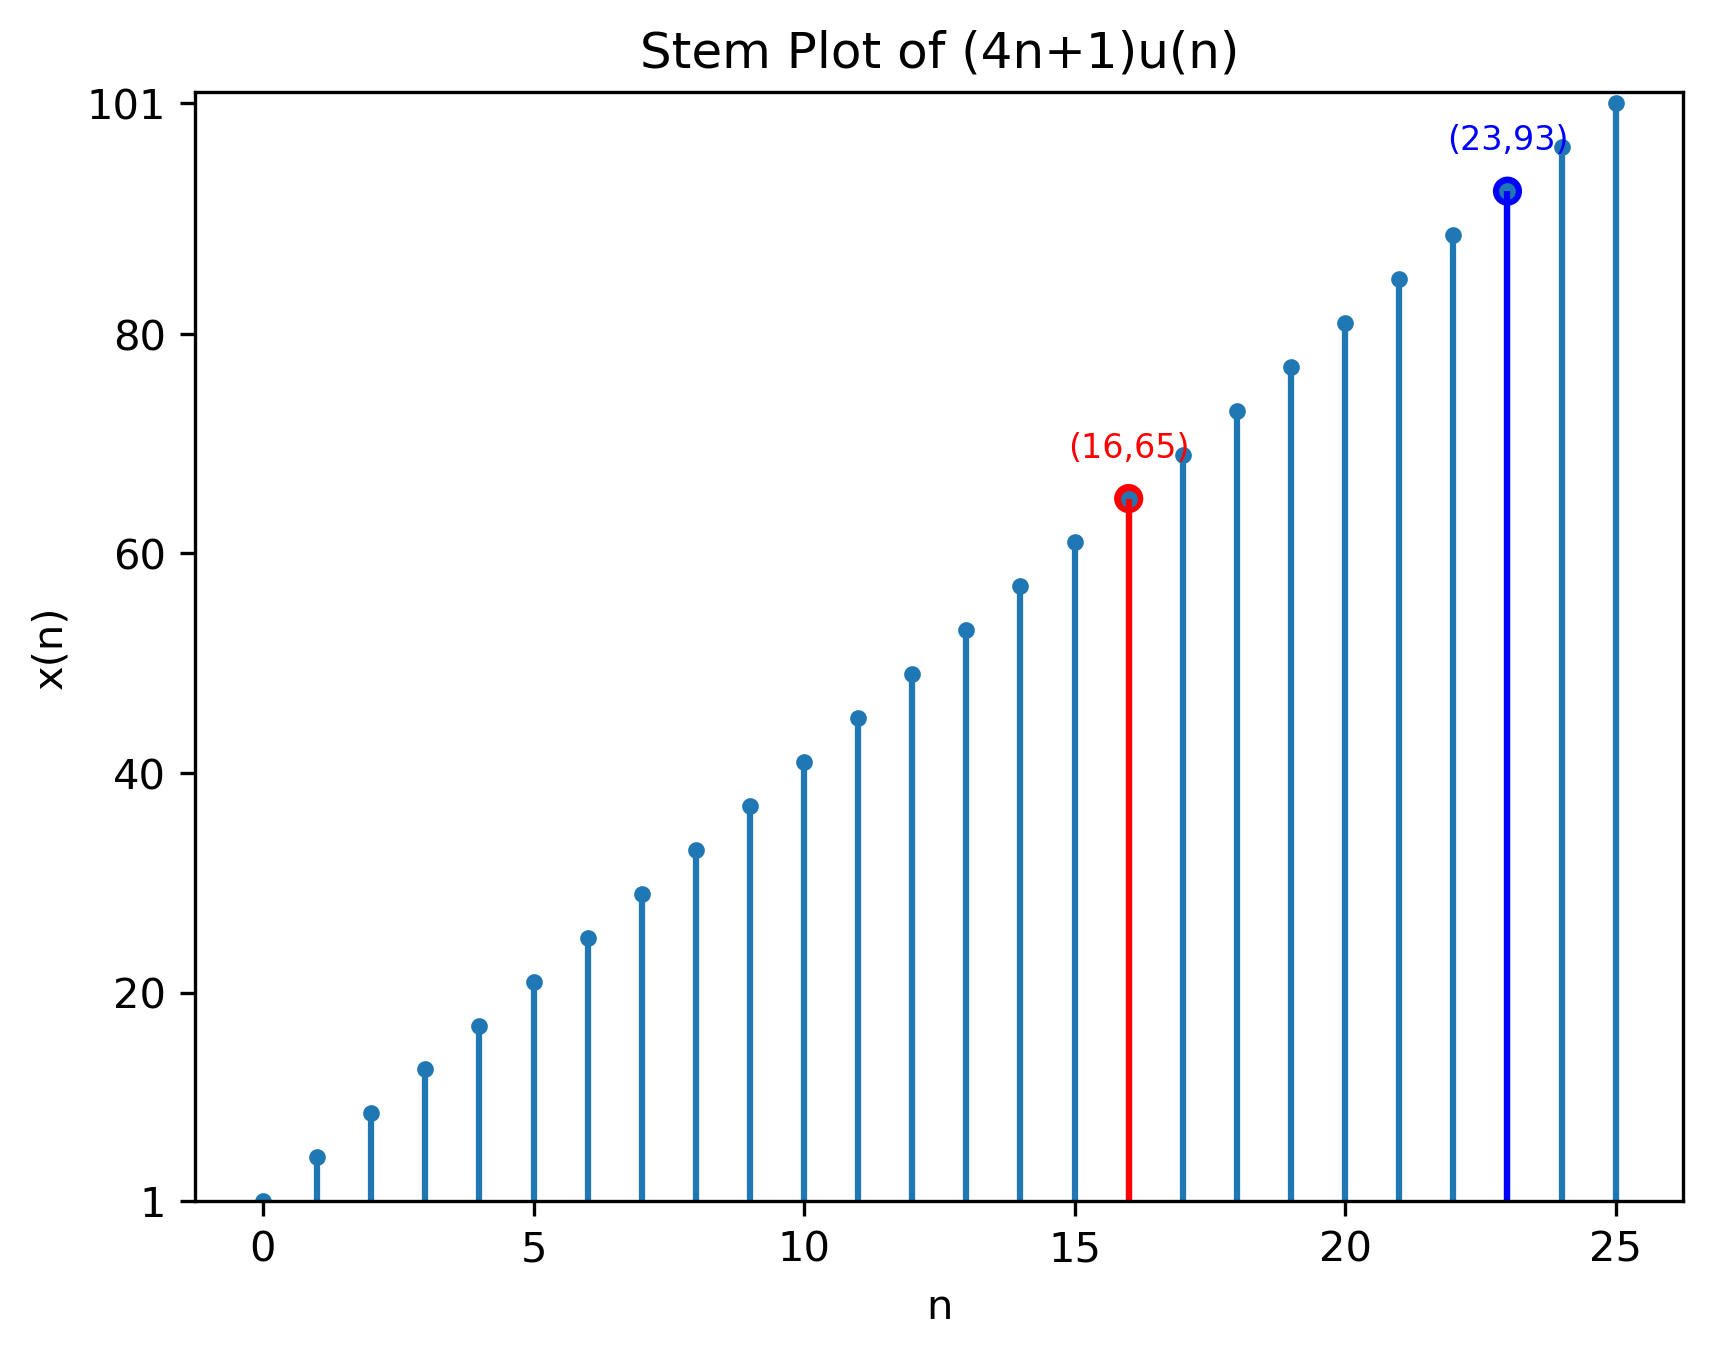
\includegraphics[width = \columnwidth]{figs/a_plot.png}
    \caption{$x(n)$ vs $n$}
    \label{fig:sw_plot}
\end{figure}



\end{document}




\pagebreak

\item The difference between any two cosecutive interior angles of a polygon is $5^\circ$.If the smallest angle is $120^\circ$,find the number of sides of polygon. \\
\solution
\input{ncert-maths/11/9/2/18/ass_1.tex}
\pagebreak
\item The $5$th,$8$th and $11$th terms of a GP are p,q and s respectively .show that $q^2=ps$ \\
\solution
\iffalse
\let\negmedspace\undefined
\let\negthickspace\undefined
\documentclass[journal,12pt,twocolumn]{IEEEtran}
\usepackage{cite}
\usepackage{amsmath,amssymb,amsfonts,amsthm}
\usepackage{algorithmic}
\usepackage{graphicx}
\usepackage{textcomp}
\usepackage{xcolor}
\usepackage{txfonts}
\usepackage{listings}
\usepackage{enumitem}
\usepackage{mathtools}
\usepackage{gensymb}
\usepackage{comment}
\usepackage[breaklinks=true]{hyperref}
\usepackage{tkz-euclide} 
\usepackage{listings}
\usepackage{gvv}                                        
\def\inputGnumericTable{}                                 
\usepackage[latin1]{inputenc}                                
\usepackage{color}                                            
\usepackage{array}                                            
\usepackage{longtable}                                       
\usepackage{calc}                                             
\usepackage{multirow}                                         
\usepackage{hhline}                                           
\usepackage{ifthen}                                           
\usepackage{lscape}

\newtheorem{theorem}{Theorem}[section]
\newtheorem{problem}{Problem}
\newtheorem{proposition}{Proposition}[section]
\newtheorem{lemma}{Lemma}[section]
\newtheorem{corollary}[theorem]{Corollary}
\newtheorem{example}{Example}[section]
\newtheorem{definition}[problem]{Definition}
\newcommand{\BEQA}{\begin{eqnarray}}
\newcommand{\EEQA}{\end{eqnarray}}
\newcommand{\define}{\stackrel{\triangle}{=}}
\theoremstyle{remark}
\newtheorem{rem}{Remark}
\begin{document}

\bibliographystyle{IEEEtran}
\vspace{3cm}

\title{11.9.3.3}
\author{EE23BTECH11065 - prem sagar}
\maketitle
\newpage

\bigskip 

\renewcommand{\thefigure}{\theenumi}
\renewcommand{\thetable}{\theenumi}
\textbf{Question}:\\ The $5$th,$8$th and $11$th terms of a GP are p,q and s respectively .show that $q^2=ps$
\\\\\textbf{solution}:
\fi
\begin{table}[!ht]
   \centering
    \renewcommand\thetable{1}
      \input{ncert-maths/11/9/3/3/tables/tables.tex}
    \caption{input parameters}
    \label{tab:11.9.3.3.1}
 \end{table}
\\ From \tabref{tab:11.9.3.3.1}:
\begin{align}
q^2&=x\brak{0}\,r^8\,x\brak{0}\,r^8
     \\ &=x\brak{0}^2\,r^{16}
\\ps&=x\brak{0}\,r^5\,x(0)\,r^{11}
       \\&=x\brak{0}^2\,r^{16}
\\\implies q^2&=ps
\end{align}
now we will find r and x\brak{0}:
\begin{align}
\frac{s}{p}&=\frac{x\brak{0}r^{11}}{x\brak{0}r^5}
\\r&=\brak{\frac{s}{p}}^\frac{1}{6} 
\\p&=x\brak{0}\brak{\frac{s}{p}}^\frac{5}{6}
\\x\brak{0}&=\frac{p^\frac{11}{6}}{s^\frac{5}{6}}
\end{align}
Applying z-Transform:
\begin{align}
     X(z) &= \frac{x\brak{0}}{1-r\,z^{-1}}\: \:,\abs{z}>\abs{r}
\\ \implies  X(z)&=\frac{p^3}{p^\frac{7}{6}s^\frac{5}{6}-q^2z^{-1}}\:,\abs{z}>\abs{\brak{\frac{q}{p}}^\frac{1}{3}}
     \end{align}    
\\\begin{figure}[ht]
   \renewcommand\thefigure{1}
    \centering
    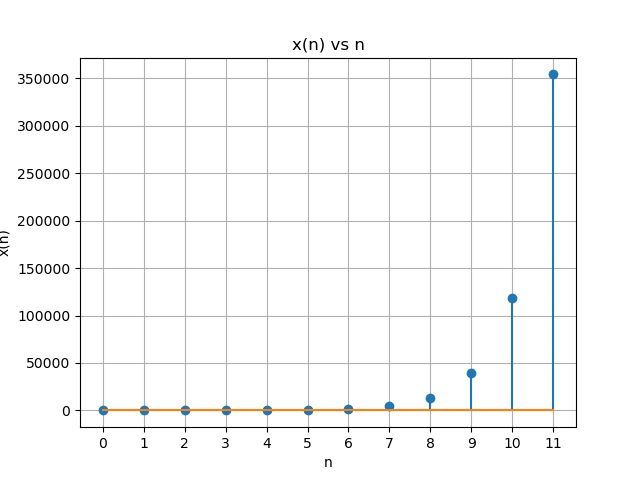
\includegraphics[width=1\linewidth]{ncert-maths/11/9/3/3/figs/figure__plot.png}
    \caption{plot x\brak{n}vs n\hspace{0.1cm}$p=486$,
    \hspace{0.1cm}$q=13122$,
    \hspace{0.1cm}$s=354294$,
    \hspace{0.1cm}$r=3$}
    \label{fig:11.9.3.3.1}
\end{figure}\\
%\end{document}

\pagebreak
\item The sum of the first four terms of an A.P. is 56. The sum of the last four terms is
 112. If its first term is 11, then find the number of terms.\\
\solution
\iffalse
\let\negmedspace\undefined
\let\negthickspace\undefined
\documentclass[journal,12pt,twocolumn]{IEEEtran}
\usepackage{cite}
\usepackage{amsmath,amssymb,amsfonts,amsthm}
\usepackage{algorithmic}
\usepackage{graphicx}
\usepackage{textcomp}
\usepackage{xcolor}
\usepackage{txfonts}
\usepackage{listings}
\usepackage{enumitem}
\usepackage{mathtools}
\usepackage{gensymb}
\usepackage{comment}
\usepackage[breaklinks=true]{hyperref}
\usepackage{tkz-euclide} 
\use-package{listings}
\usepackage{gvv}                                        
\def\inputGnumericTable{}                                 
\usepackage[latin1]{inputenc}                                
\usepackage{color}                                            
\usepackage{array}                                            
\usepackage{longtable}                                       
\usepackage{calc}                                             
\usepackage{multirow}                                         
\usepackage{hhline}                                           
\usepackage{ifthen}                                           
\usepackage{lscape}
\usepackage{caption}

\newtheorem{theorem}{Theorem}[section]
\newtheorem{problem}{Problem}
\newtheorem{proposition}{Proposition}[section]
\newtheorem{lemma}{Lemma}[section]
\newtheorem{corollary}[theorem]{Corollary}
\newtheorem{example}{Example}[section]
\newtheorem{definition}[problem]{Definition}
\newcommand{\BEQA}{\begin{eqnarray}}
\newcommand{\EEQA}{\end{eqnarray}}
\newcommand{\define}{\stackrel{\triangle}{=}}
\theoremstyle{remark}
\newtheorem{rem}{Remark}
\begin{document}

\bibliographystyle{IEEEtran}
\vspace{3cm}

\title{11.9.5}
\author{EE23BTECH11029 - Kanishk}
\maketitle

\bigskip


\textbf{Question}:\\ 
The sum of the first four terms of an A.P. is 56. The sum of the last four terms is
112. If its first term is 11, then find the number of terms.\\

\textbf{Solution}:\\ 
\fi
\begin{table}[ht]
    \centering
    \def\arraystretch{1.5}
    \input{ncert-maths/11/9/5/12/tables/TABLE.tex}
   \caption{Input Parameters}
   \label{tab:11.9.5.12}
\end{table}

\small
\begin{align}
y\brak{n}&=\sbrak{\frac{\brak{n+1}}{2}\brak{2x\brak{0}+nd}}u\brak{n}\\
\implies y(3)&=\frac{4}{2}\brak{2x\brak{0}+3d}\\
\end{align}
From \tabref{tab:11.9.5.12}:
\begin{align}
\frac{4}{2}\brak{2x\brak{0}+3d}&=56\\
2x\brak{0}+3d&=28\\
\implies d&=2
\end{align}

\begin{align}
 y\brak{n}-y\brak{n-4}&=\frac{4}{2}\brak{2x\brak{n}+3\brak{-d}}
\end{align}
From \tabref{tab:11.9.5.12}:
\begin{align}
\frac{4}{2}\brak{2x\brak{n}+3\brak{-d}}&=112\\
2x\brak{n}-3d&=56\\
\implies x\brak{n}&=31\\
x\brak{0}+\brak{n}2&=31\\
\implies n&=10
\end{align}


\begin{align}
x\brak{n}&=\brak{x\brak{0}+2n}u\brak{n}\\
\implies X\brak{z}&=\frac{x\brak{0}}{1-z^{-1}}+2\frac{z^{-1}}{\brak{1-z^{-1}}^{2}}.\quad \abs{z} > 1
\end{align}

\newpage

\begin{figure}
    
    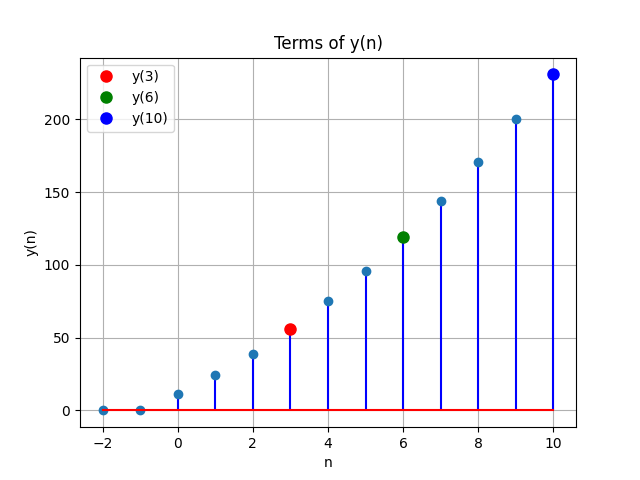
\includegraphics[width=\columnwidth]{ncert-maths/11/9/5/12//figs/fig1.png}
    \caption{Plot y(n) vs n}
\end{figure}

%\end{document}
\pagebreak
\item Find the sum to $n$ terms of the series whose $n^{th}$ term is given by $(2n-1)^2$ ? 
\solution
\pagebreak
\item If the $4^{th}$, $10^{th}$ and $16^{th}$ terms of a G.P. are $x$, $y$, and $z$, respectively. Prove that $x,\; y,\; z$ are in G.P. \\
\solution
\input{ncert-maths/11/9/3/17/A_1.tex}
\pagebreak
\item Show that the ratio of the sum of the first \(n\) terms of a geometric progression (G.P.) to the sum of terms from \((n+1)\)th to \((2n)\)th term is \(\frac{1}{r^n}\).
\solution
\pagebreak
\item A G.P consists of an even number of terms. If the sum of all terms is 5 times the sum of terms occupying odd places, then find its common ratio.\\
\solution
\documentclass[journal,12pt,twocolumn]{IEEEtran}
\usepackage{cite}
\usepackage{amsmath,amssymb,amsfonts,amsthm}
\usepackage{algorithmic}
\usepackage{graphicx}
\usepackage{textcomp}
\usepackage{xcolor}
\usepackage{txfonts}
\usepackage{listings}
\usepackage{enumitem}
\usepackage{mathtools}
\usepackage{gensymb}
\usepackage{comment}
\usepackage[breaklinks=true]{hyperref}
\usepackage{tkz-euclide}
\usepackage{gvv}
\def\inputGnumericTable{}
\usepackage[latin1]{inputenc}
\usepackage{color}
\usepackage{array}
\usepackage{longtable}
\usepackage{calc}
\usepackage{multirow}
\usepackage{hhline}
\usepackage{ifthen}
\usepackage{lscape}

\newtheorem{theorem}{Theorem}[section]
\newtheorem{problem}{Problem}
\newtheorem{proposition}{Proposition}[section]
\newtheorem{lemma}{Lemma}[section]
\newtheorem{corollary}[theorem]{Corollary}
\newtheorem{example}{Example}[section]
\newtheorem{definition}[problem]{Definition}
\newcommand{\BEQA}{\begin{eqnarray}}
\newcommand{\EEQA}{\end{eqnarray}}
\newcommand{\define}{\stackrel{\triangle}{=}}
\theoremstyle{remark}
\newtheorem{rem}{Remark}
\begin{document}

\bibliographystyle{IEEEtran}
\title{Maths Assignment}
\author{Abhignya Gogula\\
        EE23BTECH11023}
\maketitle
\section*{Problem Statement}
A G.P consists of an even number of terms. If the sum of all terms is 5 times the sum of terms occupying odd places, then find its common ratio.
\section*{Solution}
\begin{table}[h!]
\centering
\input{tables/table.tex}
\caption{Input Parameters}
\label{11.9.5.11tab1}
\end{table}
Solving the Question in time domain:
\begin{align}
x(n) &= x(0)r^{n} \\
y(n) &= x(0)\brak{\frac{r^{n+1}-1}{r-1}}u(n)
\label{eq:11.9.5.11eq1}
\end{align}
The sum of terms in odd places:
\begin{align}
x_o(n) &= x(0)r^{2n}
\end{align}
\begin{equation}
y_o(n)= x(0)\brak{\frac{r^{n+1}-1}{r^2-1}}u(n)
\label{eq:11.9.5.11eq2}
\end{equation}
Then from \eqref{eq:11.9.5.11eq1} and \eqref{eq:11.9.5.11eq2}
\begin{align}
x(0)\brak{\frac{r^{N}-1}{r-1}}u(n) &= 5\brak{x(0)\brak{\frac{r^{2M}-1}{r^2-1}}u(n)}\\
\frac{r^2-1}{r-1} &= 5\\
\text{as } r \neq 1, \quad \text{hence } r &= 4\\
\end{align}
X,Y,Xo,Yo are frequency counterparts of the above GP
\begin{align}
X(z) &= \frac{x(0)}{1-rz^{-1}} \quad \abs{z} > \abs{r}\\ 
X_o(z) &= \frac{x(0)}{1-r^{2}z^{-1}}\\
Y(z) &= \frac{x(0)}{\brak{1-rz^{-1}}\brak{1-z^{-1}}}\\
Y_o(z) &= \frac{x(0)}{\brak{1-rz^{\frac{-1}{2}}}\brak{1-z^{-1}}}
\end{align}
\end{document}


\pagebreak
\item Find the sum to indicated number of terms in the geometric progression $x^3,x^5,x^7,...n$ terms (if $x\neq\pm1$).\\
\solution
\iffalse
\let\negmedspace\undefined
\let\negthickspace\undefined
\documentclass[journal,12pt,twocolumn]{IEEEtran}
\usepackage{cite}
\usepackage{amsmath,amssymb,amsfonts,amsthm}
\usepackage{algorithmic}
\usepackage{graphicx}
\usepackage{textcomp}
\usepackage{xcolor}
\usepackage{txfonts}
\usepackage{listings}
\usepackage{enumitem}
\usepackage{mathtools}
\usepackage{gensymb}
\usepackage{comment}
\usepackage[breaklinks=true]{hyperref}
\usepackage{tkz-euclide} 
\usepackage{listings}
\usepackage{gvv}                                        
\def\inputGnumericTable{}                                 
\usepackage[latin1]{inputenc}                                
\usepackage{color}                                            
\usepackage{array}                                            
\usepackage{longtable}                                       
\usepackage{calc}                                             
\usepackage{multirow}                                         
\usepackage{hhline}                                           
\usepackage{ifthen}                                           
\usepackage{lscape}
\newtheorem{theorem}{Theorem}[section]
\newtheorem{problem}{Problem}
\newtheorem{proposition}{Proposition}[section]
\newtheorem{lemma}{Lemma}[section]
\newtheorem{corollary}[theorem]{Corollary}
\newtheorem{example}{Example}[section]
\newtheorem{definition}[problem]{Definition}
\newcommand{\BEQA}{\begin{eqnarray}}
\newcommand{\EEQA}{\end{eqnarray}}
\newcommand{\define}{\stackrel{\triangle}{=}}
\theoremstyle{remark}
\newtheorem{rem}{Remark}
\begin{document}

\bibliographystyle{IEEEtran}
\vspace{3cm}

\title{NCERT 11.9.3.Q10}
\author{EE23BTECH11224 - Sri Krishna Prabhas Yadla$^{*}$% <-this % stops a space
}
\maketitle
\newpage
\bigskip

\renewcommand{\thefigure}{\arabic{figure}}
\renewcommand{\thetable}{\arabic{table}}


\vspace{3cm}
\textbf{Question:} Find the sum to indicated number of terms in the geometric progression $x^3,x^5,x^7,...n$ terms (if $x\neq\pm1$).
\\
\solution
\fi
\input{ncert-maths/11/9/3/10/tables/11.9.3.Q10.tab1.tex}
\newline
From \tabref{tab:1.11.9.3.Q10},
\begin{align}
	X(z) &= \frac{x(0)}{1-rz^{-1}} \\
	&= \frac{x^3}{1-x^2z^{-1}} \quad \abs{z}>x^2 \\
	y(n) &= x(n) * u(n) \\
	Y(z) &= X(z)U(z) \\
	&= \frac{x^3}{(1-x^2z^{-1})(1-z^{-1})} \quad  \abs{z} > x^2 \cap \abs{z}>1\\
	&= \frac{x^3}{x^2-1}\brak{\frac{x^2}{1-x^2z^{-1}}-\frac{1}{1-z^{-1}}} \\
	u(n) &\system{Z} \frac{1}{1-z^{-1}} \quad \abs{z}>1 \\
	x^{2n+2} u(n) &\system{Z} \frac{x^2}{1-x^2z^{-1}} \quad \abs{z}>x^2
\end{align}
Taking inverse Z transform of $Y(z)$,
\begin{align}
	y(n) &= x^3\brak{\frac{x^{2n+2}-1}{x^2-1}}u(n)
\end{align}
\begin{figure}[ht!]
	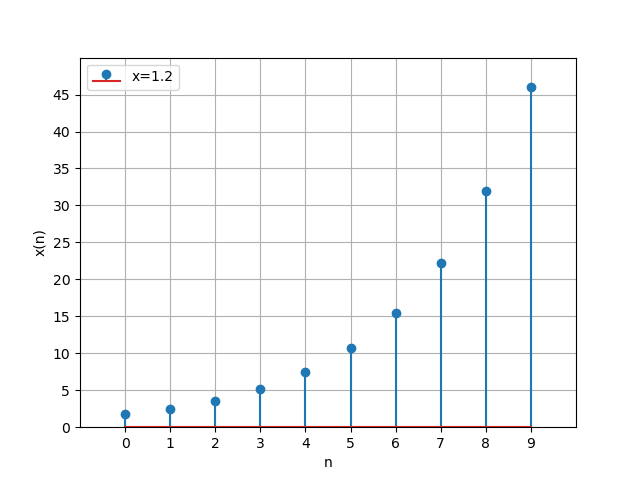
\includegraphics[width=\columnwidth]{ncert-maths/11/9/3/10/figs/plot_2.png}
	\caption{Plot of $x(n)$ for $x=1.2$}
	\label{fig:1.2}
\end{figure}

\pagebreak
\item Find sum to n terms of the following series:\\
$\frac{1}{1 \times 2} + \frac{1}{2 \times 3} + \frac{1}{3 \times 4} + \ldots$
\solution
\pagebreak
\end{enumerate}

\section{Sequences}
\begin{enumerate}[label=\thesection.\arabic*,ref=\thesection.\theenumi]
\item Find the number of terms in each of the following APs. 
\begin{enumerate}
    \item 7, 13, 19, ... 205

    \item 18, 15$\frac{1}{2}$, 13, ... -47
\end{enumerate}
\solution
\iffalse
\let\negmedspace\undefined
\let\negthickspace\undefined
\documentclass[journal,12pt,twocolumn]{IEEEtran}
\usepackage{cite}
\usepackage{amsmath,amssymb,amsfonts,amsthm}
\usepackage{algorithmic}
\usepackage{graphicx}
\usepackage{textcomp}
\usepackage{xcolor}
\usepackage{txfonts}
\usepackage{listings}
\usepackage{enumitem}
\usepackage{mathtools}
\usepackage{gensymb}
\usepackage{comment}
\usepackage[breaklinks=true]{hyperref}
\usepackage{tkz-euclide} 
\usepackage{listings}
\usepackage{gvv}                                        
\def\inputGnumericTable{}                                 
\usepackage[latin1]{inputenc}                                
\usepackage{color}                                            
\usepackage{array}                                            
\usepackage{longtable}                                       
\usepackage{calc}                                             
\usepackage{multirow}                                         
\usepackage{hhline}                                           
\usepackage{ifthen}                                           
\usepackage{lscape}
\usepackage{placeins}
\usepackage{xparse}


\newtheorem{theorem}{Theorem}[section]
\newtheorem{problem}{Problem}
\newtheorem{proposition}{Proposition}[section]
\newtheorem{lemma}{Lemma}[section]
\newtheorem{corollary}[theorem]{Corollary}
\newtheorem{example}{Example}[section]
\newtheorem{definition}[problem]{Definition}
\newcommand{\BEQA}{\begin{eqnarray}}
\newcommand{\EEQA}{\end{eqnarray}}
\newcommand{\define}{\stackrel{\triangle}{=}}
\theoremstyle{remark}
\newtheorem{rem}{Remark}



\begin{document}

\bibliographystyle{IEEEtran}
\vspace{3cm}

\Large\title{NCERT Question 10.5.2.5}
\large\author{EE23BTECH11032 - Kaustubh Parag Khachane $^{*}$% <-this % stops a space
}
\maketitle
\newpage
\bigskip

\renewcommand{\thefigure}{\theenumi}
\renewcommand{\thetable}{\theenumi}
\large\textbf{Question 10.5.2.5} : \normalsize Find the number of terms in each of the following APs. Then express each term as x\brak{n} and find the z transform, ROC and plot the graph for x\brak{n}: 
\begin{enumerate}
    \item 7, 13, 19, ... 205

    \item 18, 15$\frac{1}{2}$, 13, ... -47
\end{enumerate}


\solution
\fi
\input{ncert-maths/10/5/2/5/tables/table1}
The number of terms in the AP x\brak{n} is given by: 
\begin{align}  \label{eq:eq12}
    \frac{x\brak{n} - x\brak{0}}{d} + 1
\end{align}
\begin{align}
    &X_i(z) = \frac{x_i\brak{0}}{1 - z^{-1}} + d_i\frac{z^{-1}}{\brak{1-z^{-1}}^2} \text{ , for i=1,2} \label{eq:eq3}\\
    &\text{ROC : $\abs{z} > 1$ as it is an AP}   
\end{align}
\begin{enumerate}
    \item 
\begin{align}
x_{1}\brak{n} &= \brak{7 + \brak{n}6}u\brak{n}
\end{align}
Using the values in \tabref{tab:table0} and equation \eqref{eq:eq12},
\begin{align}
    k_1 = \frac{205 - 7}{6} + 1 = 34
\end{align}

Using the values in \tabref{tab:table0} and equation \eqref{eq:eq3} :
\begin{align}
 X_1\brak{z} = \frac{7 - z^{-1}}{\brak{1-z^{-1}}^2}
\end{align}

ROC is $\abs{z} > 1$
 
   \item
   
\begin{align}
    x_{2}\brak{n} &= \brak{18 + n\brak{-2.5}u\brak{n}}
\end{align}

Using the values in \tabref{tab:table0} and equation \eqref{eq:eq12},
\begin{align}
    k_2 = \frac{-47 - 18}{-2.5} + 1 = 27
\end{align}

Using the values in \tabref{tab:table0} and equation \eqref{eq:eq3} :
\begin{align} 
 X_2\brak{z} = \frac{18 - \brak{20.5}z^{-1}}{\brak{1 - z^{-1}}^2}
\end{align}

ROC is $\abs{z} > 1$.

\begin{figure}[h]
\centering
\begin{center}
\includegraphics[width=\columnwidth]{ncert-maths/10/5/2/5/figs/Figure_1}
\caption{Plot of $x_1\brak{n}$}
\end{center}
\end{figure}

\begin{figure}[h]
\centering
\begin{center}
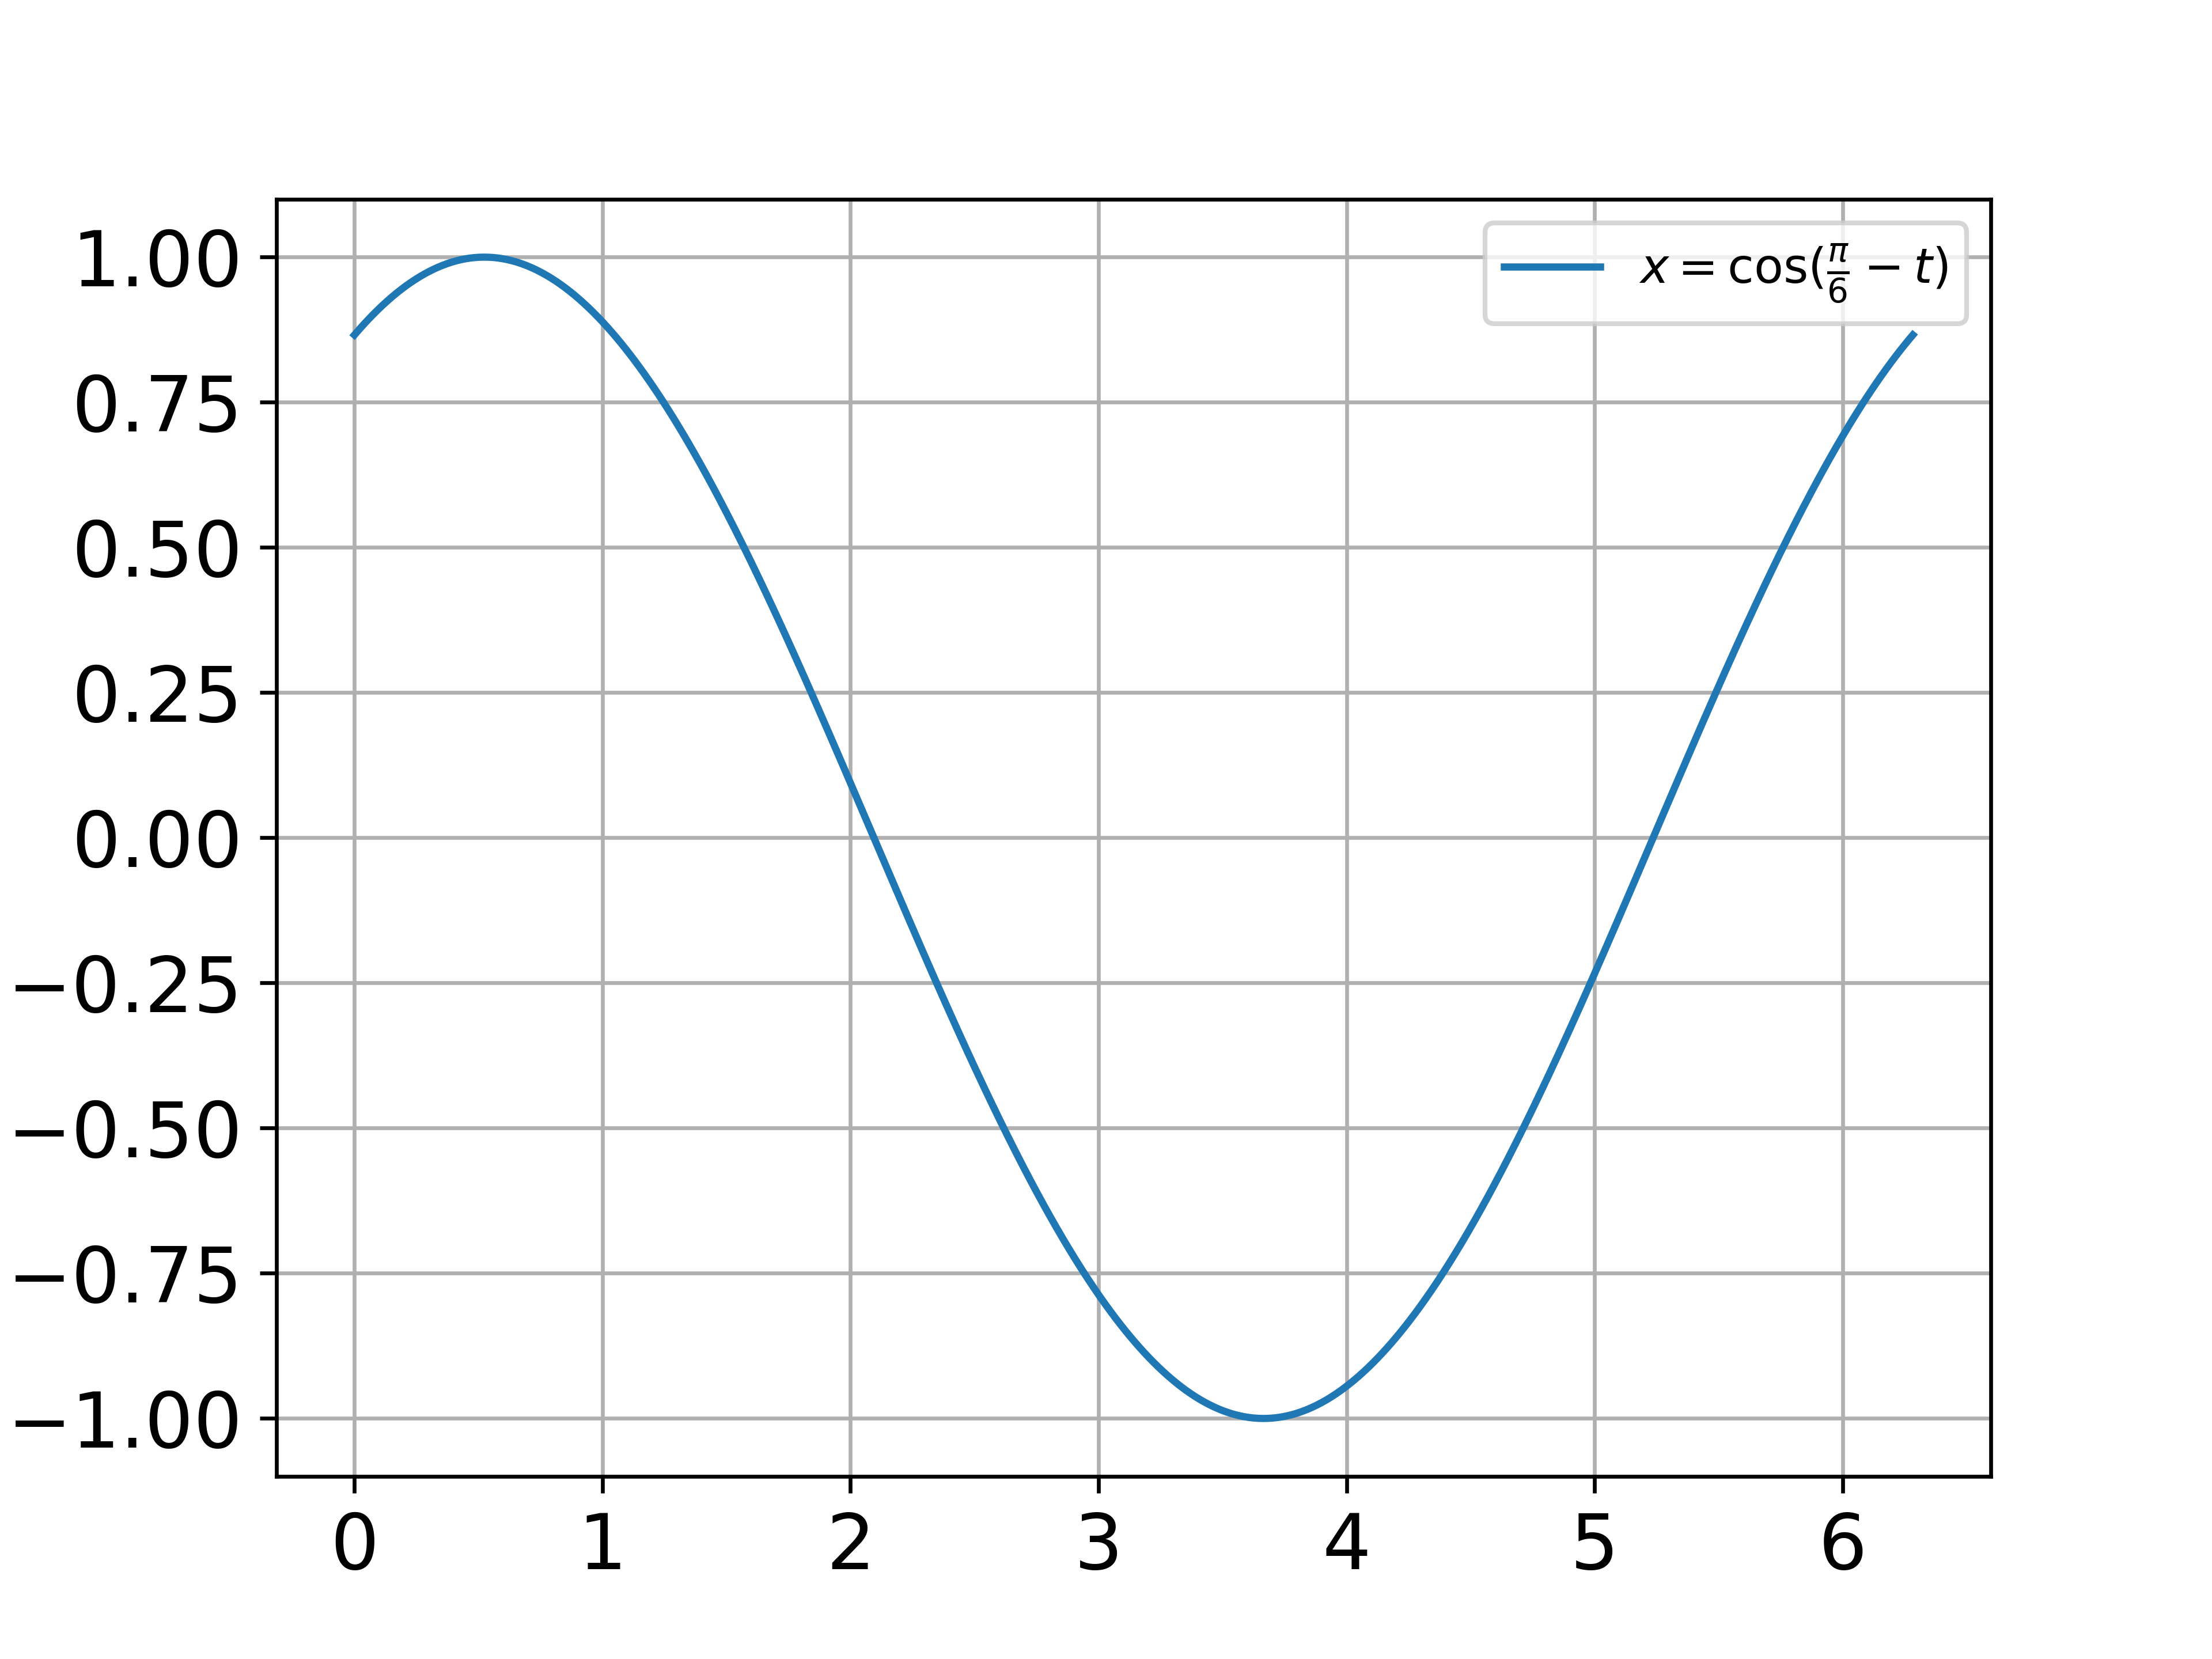
\includegraphics[width=\columnwidth]{ncert-maths/10/5/2/5/figs/Figure_2}
\caption{Plot of $x_2\brak{n}$}
\end{center}
\end{figure}

\end{enumerate}
%\end{document}

\pagebreak

\item For what value of $ n$, are the $ nth$ terms of two A.Ps: 63, 65, 67,\dots and 3, 10, 17,\dots equal?
\solution
\iffalse
\let\negmedspace\undefined
\let\negthickspace\undefined
\documentclass[journal,12pt,twocolumn]{IEEEtran}
\usepackage{cite}
\usepackage{amsmath,amssymb,amsfonts,amsthm}
\usepackage{algorithmic}
\usepackage{graphicx}
\usepackage{textcomp}
\usepackage{xcolor}
\usepackage{txfonts}
\usepackage{listings}
\usepackage{enumitem}
\usepackage{mathtools}
\usepackage{gensymb}
\usepackage{comment}
\usepackage[breaklinks=true]{hyperref}
\usepackage{tkz-euclide}
\usepackage{listings}
\usepackage{gvv}
\def\inputGnumericTable{}
\usepackage[latin1]{inputenc}
\usepackage{color}
\usepackage{array}
\usepackage{longtable}
\usepackage{calc}
\usepackage{multirow}
\usepackage{hhline}
\usepackage{ifthen}
\usepackage{lscape}

\newtheorem{theorem}{Theorem}[section]
\newtheorem{problem}{Problem}
\newtheorem{proposition}{Proposition}[section]
\newtheorem{lemma}{Lemma}[section]
\newtheorem{corollary}[theorem]{Corollary}
\newtheorem{example}{Example}[section]
\newtheorem{definition}[problem]{Definition}
\newcommand{\BEQA}{\begin{eqnarray}}
\newcommand{\EEQA}{\end{eqnarray}}
\newcommand{\define}{\stackrel{\triangle}{=}}
\theoremstyle{remark}
\newtheorem{rem}{Remark}
\begin{document}

\bibliographystyle{IEEEtran}
\vspace{3cm}

\title{NCERT Discrete 10.5.2 -15}
\author{EE23BTECH11057 - Shakunaveti Sai Sri Ram Varun$^{}$% &lt;-this % stops a space
}
\maketitle
\newpage
\bigskip

\vspace{2cm}
\textbf{Question: }
For what value of $ n$, are the $ nth$ terms of two A.Ps: 63, 65, 67,\dots and 3, 10, 17,\dots equal?\\
\vspace{0.5cm}
\textbf{Solution}:
\fi
\begin{table}[h] 
\centering
\input{ncert-maths/10/5/2/15/tables/table1}
\caption{input values}
\label{tab: Table10.5.2.15}
\end{table}
\begin{align}
x_i\brak{n} &= x\brak{0}u\brak{n} + dnu\brak{n}\\
X\brak{z} &= \frac{x\brak{0}}{1-z^{-1}} + \frac{dz^{-1}}{\brak{1-z^{-1}}^{2}} \quad |z|>1
\end{align}
\begin{enumerate}
\item
\begin{align}
x_1\brak{n} &= 63u\brak{n} + 2nu\brak{n}\\
%To find $ X_1\brak{z}$:
X_1\brak{z} &= \frac{63}{1-z^{-1}} + \frac{2z^{-1}}{\brak{1-z^{-1}}^{2}}  \quad |z|>1
\end{align}
\item
\begin{align}
x_2\brak{n} &= 3u\brak{n} + 7nu\brak{n}\\ 
%To find $ X_2\brak{z}$ :\\
X_2\brak{z} &= \frac{3}{1-z^{-1}} + \frac{7z^{-1}}{\brak{1-z^{-1}}^{2}} \quad |z|>1
\end{align}
\item

given,
\begin{align}
 x_1\brak{n} &= x_2\brak{n}\\
\therefore 63 + 2n &= 7n+3\\
\implies n &=12
\end{align}
\begin{figure}[h]
    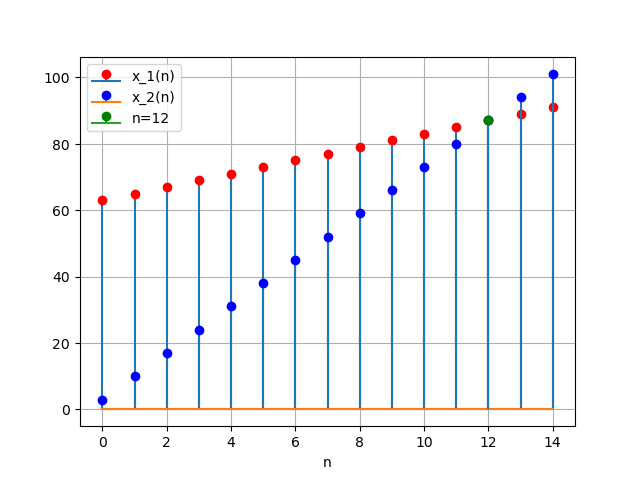
\includegraphics[width = \columnwidth]{ncert-maths/10/5/2/15/figs/Figure_1.png}
    \caption{Graphs of $ x_1\brak{n}$ and $ x_2\brak{n}$ and both are equal at $ n=12$}
    \label{fig: fig10.5.2.15}
\end{figure}
\end{enumerate}
%\end{document}

\pagebreak

\item Two APs have the same common difference.The difference between their $100${th} terms is 100,what is the difference between their $1000${th} terms?

\solution
\iffalse
\let\negmedspace\undefined
\let\negthickspace\undefined
\documentclass[journal,12pt,onecolumn]{IEEEtran}
\usepackage{cite}
\usepackage{amsmath,amssymb,amsfonts,amsthm}
\usepackage{algorithmic}
\usepackage{graphicx}
\usepackage{textcomp}
\usepackage{xcolor}
\usepackage{txfonts}
\usepackage{listings}
\usepackage{enumitem}
\usepackage{mathtools}
\usepackage{gensymb}
\usepackage{comment}
\usepackage[breaklinks=true]{hyperref}
\usepackage{tkz-euclide} 
\usepackage{listings}
\usepackage{gvv}                                        
\def\inputGnumericTable{}                                 
\usepackage[latin1]{inputenc}                                
\usepackage{color}                                            
\usepackage{array}                                            
\usepackage{longtable}                                       
\usepackage{calc}                                             
\usepackage{multirow}                                         
\usepackage{hhline}                                           
\usepackage{ifthen}                                           
\usepackage{lscape}
\newtheorem{theorem}{Theorem}[section]
\newtheorem{problem}{Problem}
\newtheorem{proposition}{Proposition}[section]
\newtheorem{lemma}{Lemma}[section]
\newtheorem{corollary}[theorem]{Corollary}
\newtheorem{example}{Example}[section]
\newtheorem{definition}[problem]{Definition}
\newcommand{\BEQA}{\begin{eqnarray}}
\newcommand{\EEQA}{\end{eqnarray}}
\newcommand{\define}{\stackrel{\triangle}{=}}
\theoremstyle{remark}
\newtheorem{rem}{Remark}
\begin{document}
\bibliographystyle{IEEEtran}
\vspace{3cm}
\title{NCERT 11.9.2 16Q}
\author{EE23BTECH11021 - GANNE GOPI CHANDU$^{*}$% <-this % stops a space
}
\maketitle
\bigskip
\renewcommand{\thefigure}{\theenumi}
\renewcommand{\thetable}{\theenumi}
\bibliographystyle{IEEEtran}
\textbf{Question}\\
Between 1 and 31, m numbers have been inserted in such a way that the resulting sequence is an A.P. and 
the ratio of 7 th and (m - 1) th numbers is 5:9. Find the value of m.\\
\textbf{Solution}\\
\fi
\begin{table}[!h]
\begin{center}
\renewcommand\thetable{1}
\begin{tabular}{ |c|c|c| } 
  \hline
    Symbol & Value & description \\ 
  \hline
  $x(0)$ & $1$ & First term of A.P  \\ 
  \hline
  $x(n)$ & $31$ & $\brak{n+1}\text{th}$ term \\
  \hline
  $\frac{x\brak{7}}{x\brak{m-1}}$ & $\frac{5}{9}$ & ratio of $7$ th  and $(m-1)$ th numbers\\ 
  \hline
  $n$ & $m+2$ & number of terms \\
  \hline
\end{tabular}
\end{center}
\caption{}
\end{table}\\
The last term is
\begin{align}
x(n)&=x(0)+\brak{n}d\\
\implies31 &= 1 + \brak{m + 1}d \\
\implies30 &= \brak{m + 1}d \\
\implies\frac{30}{m + 1} &= d \label{eq11.9.2.4}
\end{align}
Now $7$th and $\brak{m-1}$th terms
\begin{align}
x\brak{7} &= x(0) + 7d\label{eq11.9.2.5}\\
x\brak{m-1} &= x(0) + \brak{m-1}d\label{eq11.9.2.6}
\end{align}
From  equations \eqref{eq11.9.2.5} and \eqref{eq11.9.2.6}\\
\begin{align}
   \frac{x(0) + 7d}{x(0) + \brak{m-1}d} &= \frac{5}{9} \label{eq11.9.2.7}
\end{align}
Substituting  \eqref{eq11.9.2.4} in \eqref{eq11.9.2.7}\\
\begin{align}
\implies \frac{1+7\brak{{\frac{30}{m+1}}}}{1+\brak{{m-1}}\brak{\frac{30}{m+1}}} &= \frac{5}{9} \\
\implies \frac{m+1+210}{m+1+30m-30} &= \frac{5}{9}\\
\implies \frac{m+181}{31m-29} &= \frac{5}{9}\\
\implies 9m+1899 &=155m-145\\
\implies 155m-9m &=1899+145\\
\implies 146m &=2044\\
\implies m &=14
\end{align}
Therefore, $m = 14$ .\\
 \text{General term of AP is} \\
\begin{align}
    x\brak{n}&=\brak{2n+1}u(n)\\
    x\brak{n}&=\brak{2n}u\brak{n}+u\brak{n}
\end{align}
\begin{figure}
    \centering
    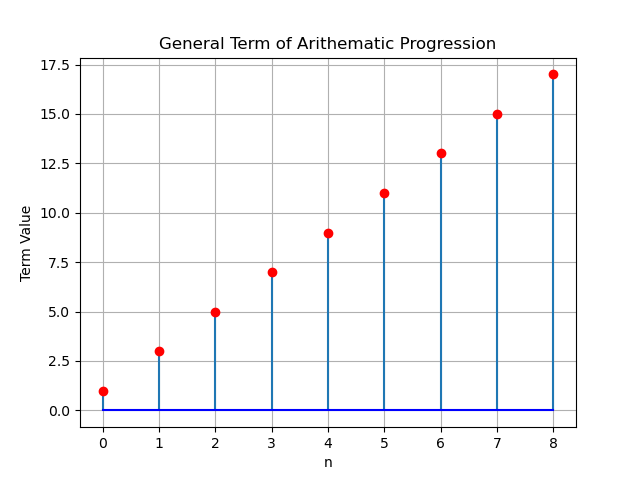
\includegraphics[width=1.0\linewidth]{ncert-maths/11/9/2/16/figs/test.png}
    \caption{Plot of x(n) vs n}
    \label{fig:1}
\end{figure}\\
The Z-Transform is\\
\begin{align}
    X\brak{z}&=2\brak{\dfrac{z}{\brak{z-1}^{2}}}+U\brak{z}\\
    &=\dfrac{2z}{\brak{z-1}^{2}}+\dfrac{1}{1-z^{-1}}\\
    X\brak{z}&=\dfrac{z^2+z}{\brak{z-1}^{2}} \quad{|z|>1}
\end{align}


\item Check whether -150 is a term of the AP: 11,8,5,2,....

 \solution
 \iffalse
\let\negmedspace\undefined
\let\negthickspace\undefined
\documentclass[journal,12pt,onecolumn]{IEEEtran}
\usepackage{cite}
\usepackage{amsmath,amssymb,amsfonts,amsthm}
\usepackage{algorithmic}
\usepackage{graphicx}
\usepackage{textcomp}
\usepackage{xcolor}
\usepackage{txfonts}
\usepackage{listings}
\usepackage{enumitem}
\usepackage{mathtools}
\usepackage{gensymb}
\usepackage{comment}
\usepackage[breaklinks=true]{hyperref}
\usepackage{tkz-euclide} % loads  TikZ and tkz-base
\usepackage{listings}
\usepackage[latin1]{inputenc}                                
\usepackage{color}                                            
\usepackage{array}                                            
\usepackage{longtable}                                       
\usepackage{calc}                                             
\usepackage{multirow}                                         
\usepackage{hhline}                                           
\usepackage{ifthen}                                           
\usepackage{lscape}
\usepackage{caption}


\newtheorem{theorem}{Theorem}[section]
\newtheorem{problem}{Problem}
\newtheorem{proposition}{Proposition}[section]
\newtheorem{lemma}{Lemma}[section]
\newtheorem{corollary}[theorem]{Corollary}
\newtheorem{example}{Example}[section]
\newtheorem{definition}[problem]{Definition}
%\newtheorem{thm}{Theorem}[section] 
%\newtheorem{defn}[thm]{Definition}
%\newtheorem{algorithm}{Algorithm}[section]
%\newtheorem{cor}{Corollary}
\newcommand{\BEQA}{\begin{eqnarray}}
\newcommand{\EEQA}{\end{eqnarray}}
\newcommand{\define}{\stackrel{\triangle}{=}}
\theoremstyle{remark}
\newtheorem{rem}{Remark}
%\bibliographystyle{ieeetr}

\begin{document}

%
\providecommand{\pr}[1]{\ensuremath{\Pr\left(#1\right)}}
\providecommand{\prt}[2]{\ensuremath{p_{#1}^{\left(#2\right)} }}        % own macro for this question
\providecommand{\qfunc}[1]{\ensuremath{Q\left(#1\right)}}
\providecommand{\sbrak}[1]{\ensuremath{{}\left[#1\right]}}
\providecommand{\lsbrak}[1]{\ensuremath{{}\left[#1\right.}}
\providecommand{\rsbrak}[1]{\ensuremath{{}\left.#1\right]}}
\providecommand{\brak}[1]{\ensuremath{\left(#1\right)}}
\providecommand{\lbrak}[1]{\ensuremath{\left(#1\right.}}
\providecommand{\rbrak}[1]{\ensuremath{\left.#1\right)}}
\providecommand{\cbrak}[1]{\ensuremath{\left\{#1\right\}}}
\providecommand{\lcbrak}[1]{\ensuremath{\left\{#1\right.}}
\providecommand{\rcbrak}[1]{\ensuremath{\left.#1\right\}}}
\newcommand{\sgn}{\mathop{\mathrm{sgn}}}
\providecommand{\abs}[1]{\left\vert#1\right\vert}
\providecommand{\res}[1]{\Res\displaylimits_{#1}} 
\providecommand{\norm}[1]{\left\lVert#1\right\rVert}
%\providecommand{\norm}[1]{\lVert#1\rVert}
\providecommand{\mtx}[1]{\mathbf{#1}}
\providecommand{\mean}[1]{E\left[ #1 \right]}
\providecommand{\cond}[2]{#1\middle|#2}
\providecommand{\fourier}{\overset{\mathcal{F}}{ \rightleftharpoons}}
\newenvironment{amatrix}[1]{%
  \left(\begin{array}{@{}*{#1}{c}|c@{}}
}{%
  \end{array}\right)
}
%\providecommand{\hilbert}{\overset{\mathcal{H}}{ \rightleftharpoons}}
%\providecommand{\system}{\overset{\mathcal{H}}{ \longleftrightarrow}}
        %\newcommand{\solution}[2]{\textbf{Solution:}{#1}}
\newcommand{\solution}{\noindent \textbf{Solution: }}
\newcommand{\cosec}{\,\text{cosec}\,}
\providecommand{\dec}[2]{\ensuremath{\overset{#1}{\underset{#2}{\gtrless}}}}
\newcommand{\myvec}[1]{\ensuremath{\begin{pmatrix}#1\end{pmatrix}}}
\newcommand{\mydet}[1]{\ensuremath{\begin{vmatrix}#1\end{vmatrix}}}
\newcommand{\myaugvec}[2]{\ensuremath{\begin{amatrix}{#1}#2\end{amatrix}}}
\providecommand{\rank}{\text{rank}}
\providecommand{\pr}[1]{\ensuremath{\Pr\left(#1\right)}}
\providecommand{\qfunc}[1]{\ensuremath{Q\left(#1\right)}}
        \newcommand*{\permcomb}[4][0mu]{{{}^{#3}\mkern#1#2_{#4}}}
\newcommand*{\perm}[1][-3mu]{\permcomb[#1]{P}}
\newcommand*{\comb}[1][-1mu]{\permcomb[#1]{C}}
\providecommand{\qfunc}[1]{\ensuremath{Q\left(#1\right)}}
\providecommand{\gauss}[2]{\mathcal{N}\ensuremath{\left(#1,#2\right)}}
\providecommand{\diff}[2]{\ensuremath{\frac{d{#1}}{d{#2}}}}
\providecommand{\myceil}[1]{\left \lceil #1 \right \rceil }
\newcommand\figref{Fig.~\ref}
\newcommand\tabref{Table~\ref}
\newcommand{\sinc}{\,\text{sinc}\,}
\newcommand{\rect}{\,\text{rect}\,}
%%
%       %\newcommand{\solution}[2]{\textbf{Solution:}{#1}}
%\newcommand{\solution}{\noindent \textbf{Solution: }}
%\newcommand{\cosec}{\,\text{cosec}\,}
%\numberwithin{equation}{section}
%\numberwithin{equation}{subsection}
%\numberwithin{problem}{section}
%\numberwithin{definition}{section}
%\makeatletter
%\@addtoreset{figure}{problem}
%\makeatother

%\let\StandardTheFigure\thefigure
\let\vec\mathbf

\bibliographystyle{IEEEtran}

\vspace{3cm}
\title{Assignment}
\author{EE23BTECH11001 - Aashna Sahu}
\maketitle
\bigskip

\renewcommand{\thefigure}{\theenumi}
\renewcommand{\thetable}{\theenumi}
%\renewcommand{\theequation}{\theenumi}
Q:Check whether -150 is a term of the AP: 11,8,5,2,....

 \solution
 \fi

\begin{align}
x(n)&=x(0)+nd\\
n&=\frac{x(n)-x(0)}{d}
\end{align}
\begin{align}
x(n)-x(0) &\equiv 0 \pmod{d}
\end{align}
On substitutings values\\
\begin{align}
-161 &\equiv 2 \pmod{-3}
\end{align}
Thus -150 is not a term of the given AP.
\begin{align}
 \boxed{x(n)=(11-3n)\times u(n)}   
\end{align}

\begin{align}
   X(z)&=\frac{11}{1-z^{-1}}-\frac{3z^{-1}}{(1-z^{-1})^2}\quad
    |z|>1
\end{align}

    \begin{table}[h]
    \centering
    
        \input{ncert-maths/10/5/2/6/tables/table1.tex}
        
    \caption{Input parameters}
    \label{tab:Table10.5.2.6}
\end{table}
\newpage
\begin{figure}[h]
  \centering
  \includegraphics[width=1.2\columnwidth]{ncert-maths/10/5/2/6/figs/Figure_1.png}
  \caption{Representation of x(n)}
  \label{fig:fig10.5.2.6}
\end{figure}
%\end{document}

 \pagebreak

 \item Write the first five terms of the sequence \(a_n = \frac{n(n^2+5)}{4}\).

\solution
\input{ncert-maths/11/9/1/6/file1.tex}
\pagebreak

\item
\begin{enumerate}
\item 30th term of the AP: 10, 7, 4, $\ldots$ is 
\item 11th term of the AP: $-3, -\frac{1}{2}, 2, \ldots$ is
\end{enumerate}
\solution
\input{ncert-maths/10/5/2/2/c.tex}

\pagebreak
\item Write the first five terms of the sequence whose nth term is $\frac{2n-3}{6}$ and obtain the Z transform of the series
\solution
\input{ncert-maths/11/9/1/4/d.tex}
\pagebreak
 \item For what values of x, the numbers $-\frac{2}{7}\,,x,-\frac{7}{2}\,$ are in G.P ?

\solution
\iffalse
\let\negmedspace\undefined
\let\negthickspace\undefined
\documentclass[journal,12pt,twocolumn]{IEEEtran}
\usepackage{cite}
\usepackage{amsmath,amssymb,amsfonts,amsthm}
\usepackage{algorithmic}
\usepackage{graphicx}
\usepackage{textcomp}
\usepackage[justification=centering]{caption}
\usepackage{xcolor}
\usepackage{txfonts}
\usepackage{listings}
\usepackage{enumitem}
\usepackage{mathtools}
\usepackage{gensymb}
\usepackage{comment}
\usepackage[breaklinks=true]{hyperref}
\usepackage{tkz-euclide} 
\usepackage{listings}
\usepackage{gvv}                                        
\def\inputGnumericTable{}                                 
\usepackage[latin1]{inputenc}                                
\usepackage{color}                                            
\usepackage{array}                                            
\usepackage{longtable}                                       
\usepackage{calc}                                             
\usepackage{multirow}                                         
\usepackage{hhline}                                           
\usepackage{ifthen}                                           
\usepackage{lscape}

\newtheorem{theorem}{Theorem}[section]
\newtheorem{problem}{Problem}
\newtheorem{proposition}{Proposition}[section]
\newtheorem{lemma}{Lemma}[section]
\newtheorem{corollary}[theorem]{Corollary}
\newtheorem{example}{Example}[section]
\newtheorem{definition}[problem]{Definition}
\newcommand{\BEQA}{\begin{eqnarray}}
\newcommand{\EEQA}{\end{eqnarray}}
\newcommand{\define}{\stackrel{\triangle}{=}}
\theoremstyle{remark}
\newtheorem{rem}{Remark}
\begin{document}

\bibliographystyle{IEEEtran}
\vspace{3cm}

\title{11.9.3.6}
\author{EE23BTECH11022 - G DILIP REDDY}
\maketitle
\newpage

\bigskip

\renewcommand{\thefigure}{\theenumi}
\renewcommand{\thetable}{\theenumi}
\textbf{Question}:\\
For what values of x, the numbers $-\frac{2}{7}\,,x,-\frac{7}{2}\,$ are in G.P ?
\\\\
\textbf{Solution: }\\
\fi
\begin{table}[h]
    \centering
    \renewcommand\thetable{1}
    \input{ncert-maths/11/9/3/6/tables/Table.Tex}
    \caption{Variables Used}
    \label{tab:table_11.9.3.6}
\end{table}
Let $r$ be the common ratio\\
From \tabref{tab:table_11.9.3.6}:
\begin{align}
\implies \frac{x}{\brak{-\frac{2}{7}\,}}\,&= \frac{\brak{-\frac{7}{2}\,}}{x}\,=r \\
x^2&=\brak{-\frac{2}{7}\,}\cdot\brak{-\frac{7}{2}\,}\\
x&=\pm 1\\
\implies r&=\pm \frac{7}{2}\,\\\notag
\end{align}
The signal corresponding to this is 
\begin{align}
x(n)=\brak{-\frac{2}{7}}\brak{\pm \frac{7}{2}}^n\,u(n)
\end{align}
Applying z-Transform :
\begin{align}
\implies X_1(z)&=\brak{\frac{1}{7}}\brak{\frac{4}{7z^{-1}+2}\,}
\quad \abs{z}>\frac{7}{2}\\
\implies X_2(z)&=\brak{\frac{1}{7}}\brak{\frac{4}{7z^{-1}-2}\,}
\quad \abs{z}>\frac{7}{2}
\end{align}
\begin{figure}[h]
    \renewcommand\thefigure{1}
    \centering
    \captionsetup{justification=centering}
    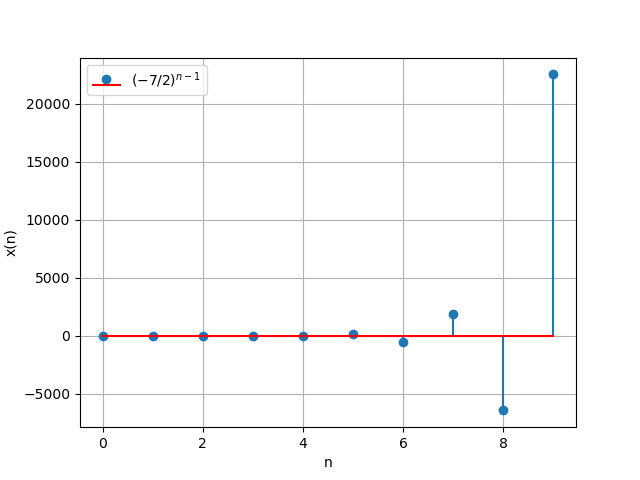
\includegraphics[width=1.1\linewidth]{ncert-maths/11/9/3/6/figs/graph1.png}
    \caption{Stem Plot of $x_1$(n)}
    \label{stemplot1}
\end{figure}
\begin{figure}[h]
    \renewcommand\thefigure{2}
    \centering
    \captionsetup{justification=centering}
    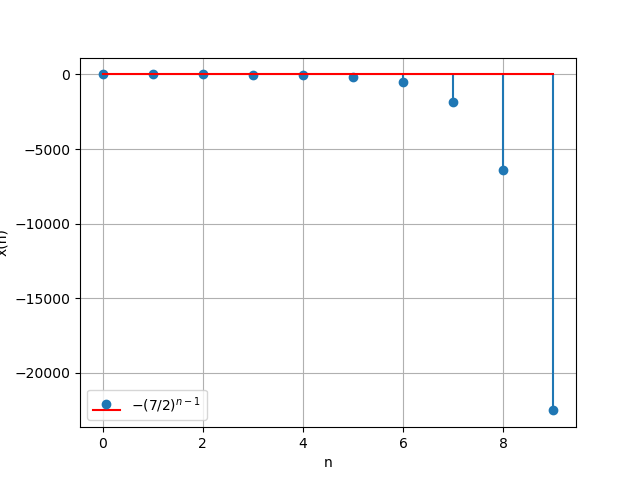
\includegraphics[width=1.1\linewidth]{ncert-maths/11/9/3/6/figs/graph2.png}
    \caption{Stem Plot of $x_2(n)$}
    \label{stemplot2}
\end{figure}
%\end{document}

\pagebreak

\item Find the $20^{th}$ and $n^{th}$ terms of the G.P $\frac{5}{2}$, $\frac{5}{4}$, $\frac{5}{8}$,.....

\solution
% \iffalse
\let\negmedspace\undefined
\let\negthickspace\undefined
\documentclass[journal,12pt,twocolumn]{IEEEtran}
\usepackage{cite}
\usepackage{amsmath,amssymb,amsfonts,amsthm}
\usepackage{algorithmic}
\usepackage{graphicx}
\usepackage{textcomp}
\usepackage{xcolor}
\usepackage{txfonts}
\usepackage{listings}
\usepackage{enumitem}
\usepackage{mathtools}
\usepackage{gensymb}
\usepackage{comment}
\usepackage[breaklinks=true]{hyperref}
\usepackage{tkz-euclide} 
\usepackage{listings}
\usepackage{gvv}                                        
\def\inputGnumericTable{}                                 
\usepackage[latin1]{inputenc}                                
\usepackage{color}                                            
\usepackage{array}                                            
\usepackage{longtable}                                       
\usepackage{calc}                                             
\usepackage{multirow}                                         
\usepackage{hhline}                                           
\usepackage{ifthen}                                           
\usepackage{lscape}
\usepackage{caption}
\newtheorem{theorem}{Theorem}[section]
\newtheorem{problem}{Problem}
\newtheorem{proposition}{Proposition}[section]
\newtheorem{lemma}{Lemma}[section]
\newtheorem{corollary}[theorem]{Corollary}
\newtheorem{example}{Example}[section]
\newtheorem{definition}[problem]{Definition}
\newcommand{\BEQA}{\begin{eqnarray}}
\newcommand{\EEQA}{\end{eqnarray}}
\newcommand{\define}{\stackrel{\triangle}{=}}
\theoremstyle{remark}
\newtheorem{rem}{Remark}
\begin{document}
\parindent 0px
\bibliographystyle{IEEEtran}
\vspace{3cm}

\title{NCERT 11.9.3 1Q}
\author{EE23BTECH11013 - Avyaaz$^{*}$% <-this % stops a space
}
\maketitle
\newpage
\bigskip

\renewcommand{\thefigure}{\arabic{figure}}
\renewcommand{\thetable}{\arabic{table}}
\large\textbf{\textsl{Question:}}
Find the $20^{th}$ and $n^{th}$ terms of the G.P $\frac{5}{2}$, $\frac{5}{4}$, $\frac{5}{8}$,.....

\solution
 \begin{table}[htbp]
     \centering
     \setlength{\extrarowheight}{8pt}
    \input{tables/table1}
     \caption{Parameters}
     \label{tab:table1}
 \end{table} 

% \begin{align}
%    x(n) = \dfrac{5}{2}\left(\dfrac{1}{2}\right)^n 
% \end{align}

% \begin{align}
% 	x \brak{n} & \system{Z} X \brak{z} \\
%    % x(n) &=\dfrac{5}{2}\left(\dfrac{1}{2}\right)^n u(n) \\
%     \therefore X(z) &= \sum_{n=-\infty}^{\infty}x(n)z^{-n}\label{eq:z-transform}  
% \end{align}
% Here, 
%          $    u(n) = \begin{cases}
%                 0 &\text{for } n < 0 \\
%                 1 & \text{for } n \geq 0
%             \end{cases}$       
 
%  \vspace{1cm}
From \tabref{tab:table1}:
\(Z\)-Transform of \(x(n)\):
\begin{align}
% \implies X(z) &= \sum_{n=-\infty}^{\infty}\left(\dfrac{5}{2}\left(\dfrac{1}{2}\right)^n u(n)\right) z^{-n} \\
 % \implies X(z) &= \dfrac{5}{2}\sum_{n=0}^{\infty}\left(\dfrac{z
 % ^{-1}}{2}\right)^n \\
\implies X(z) &=\dfrac{5}{2}\left(\dfrac{1}{1-\frac{z^{-1}}{2}}\right) ;\cbrak{z\in\mathbb{C} : |z|>\dfrac{1}{2}}
\end{align}

\begin{figure}[ht]
    \centering
    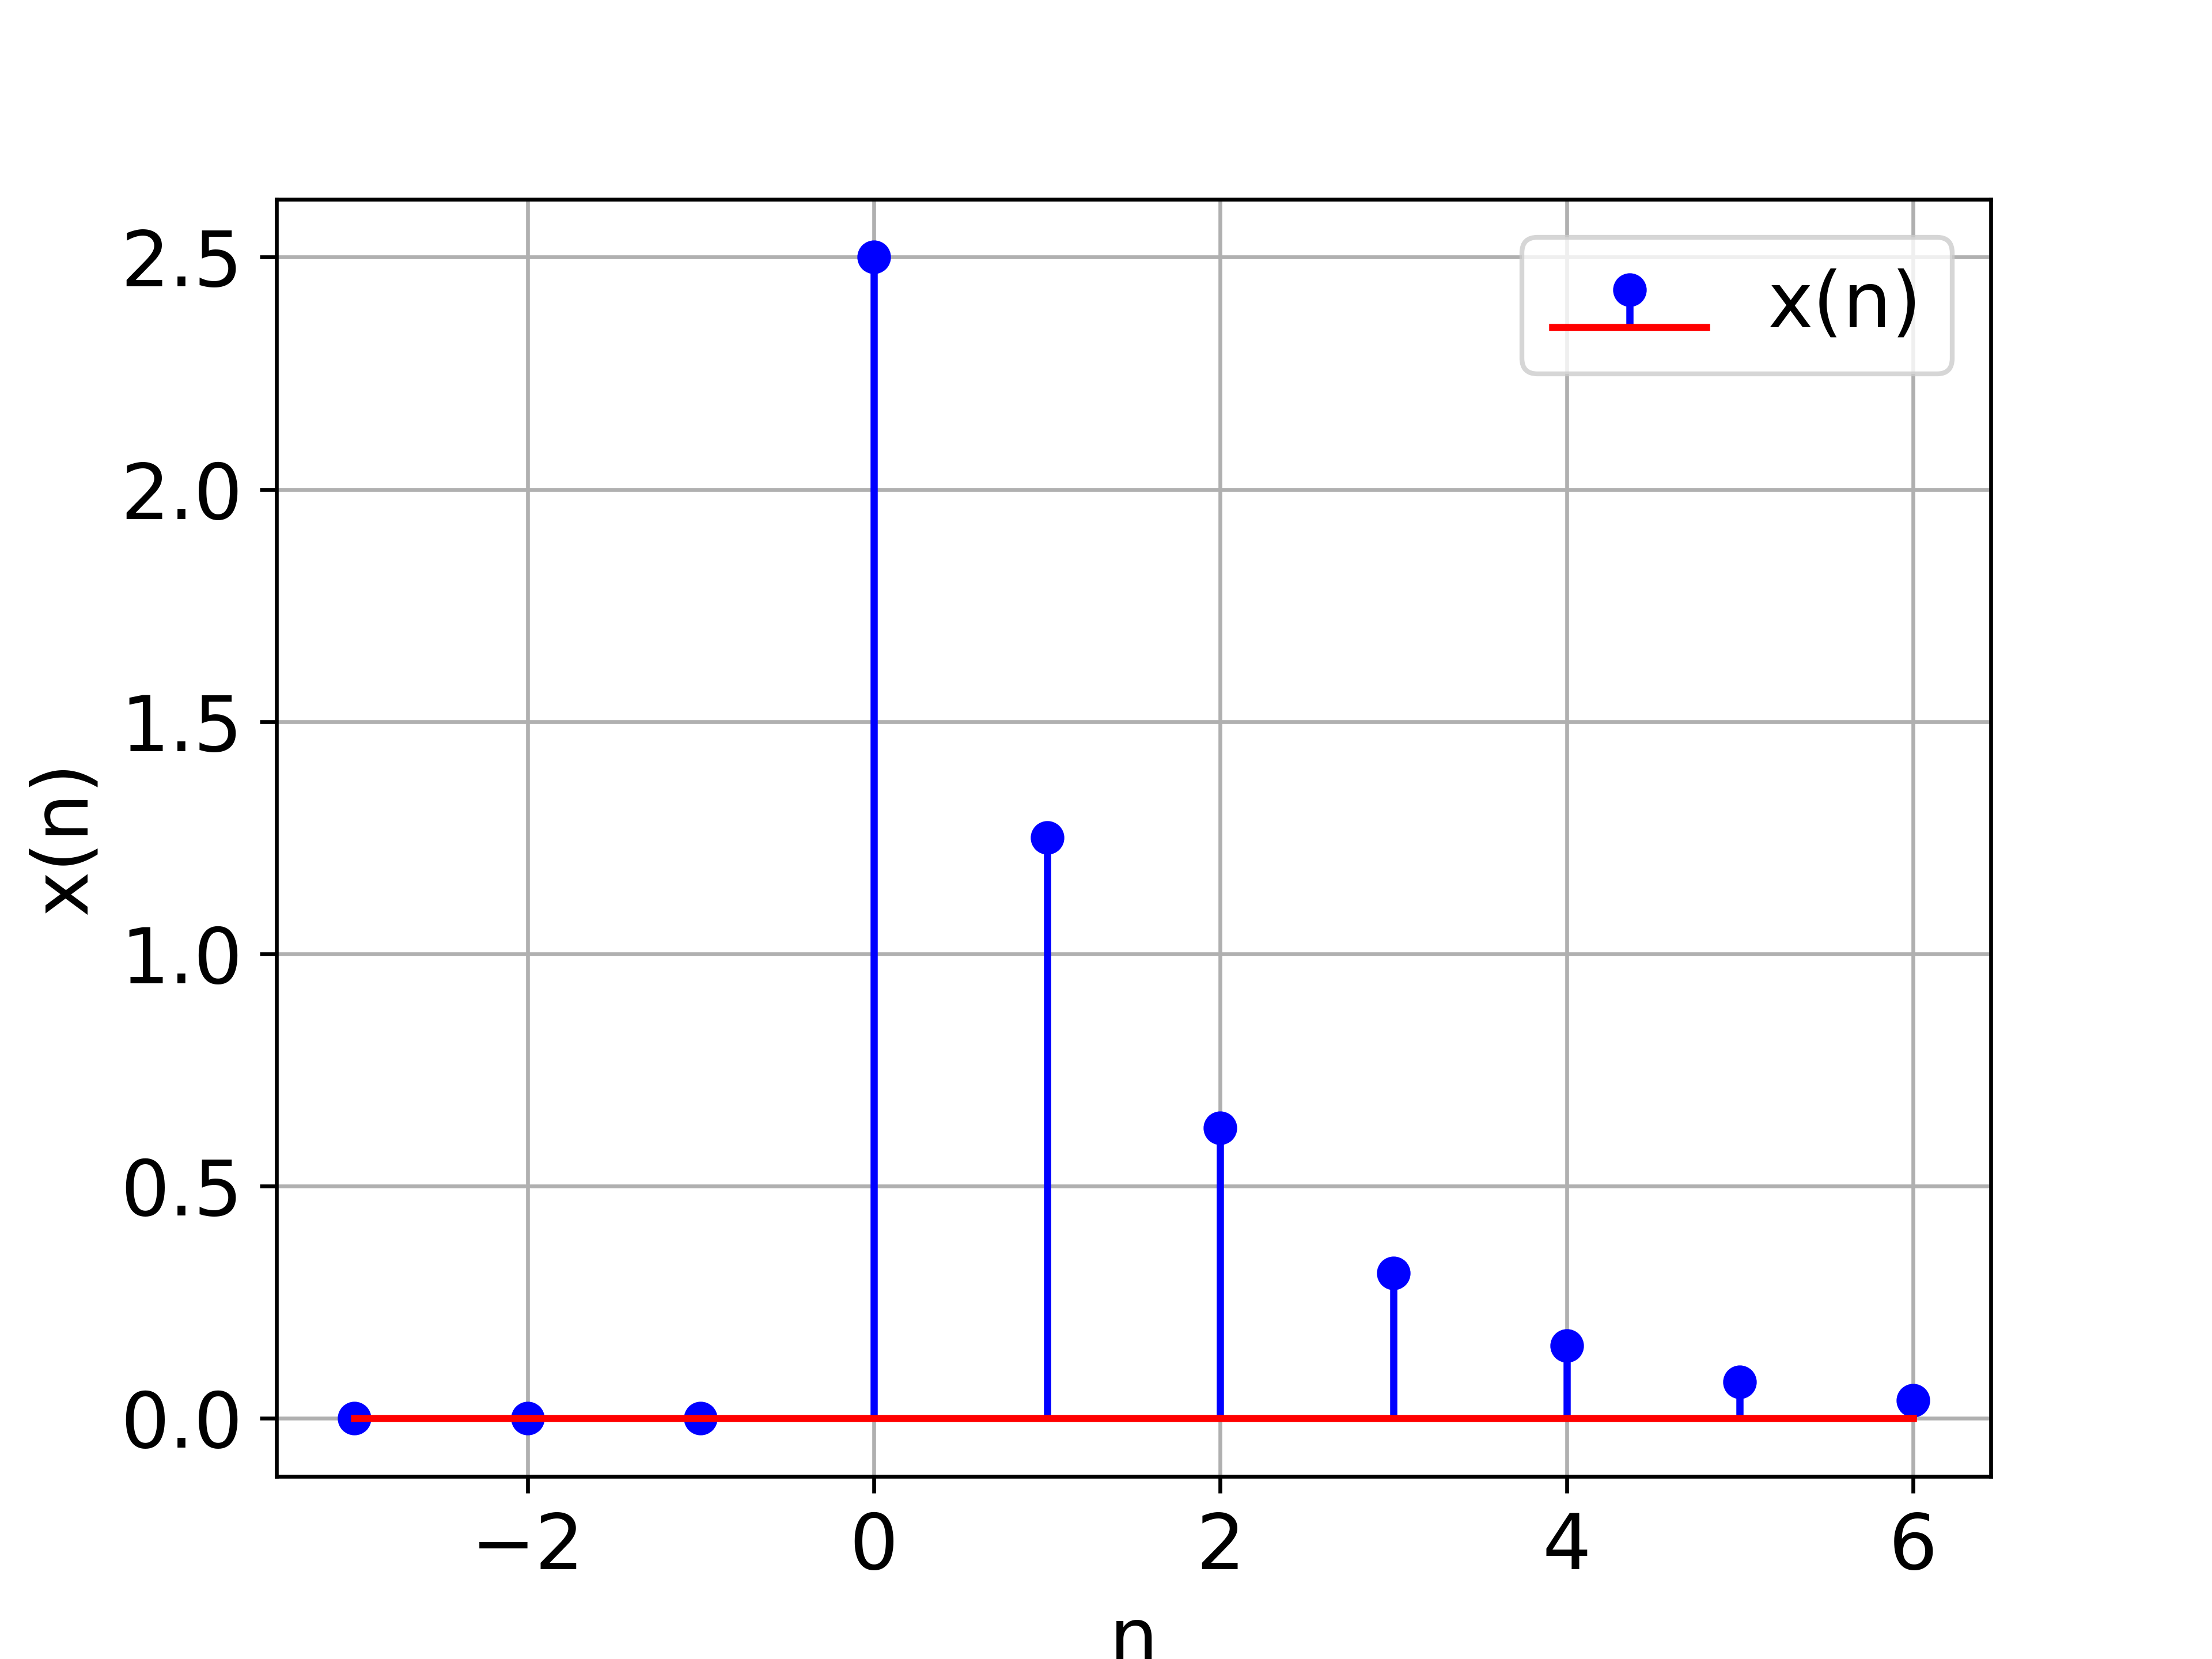
\includegraphics[width = \columnwidth]{figs/stem_plot.png}
    \caption{}
    \label{fig:graph1}
\end{figure} 

\bibliographystyle{IEEEtran}
\end{document}

\pagebreak

\item 
Which term of the following sequences:\\
(a) 2,$2\sqrt{2}$,4\dots is 128
\quad(b) $\sqrt{3}$,3,$3\sqrt{3}$\dots is 729\\
(c) $\frac{1}{3}$,$\frac{1}{9}$,$\frac{1}{27}$\dots is $\frac{1}{19683}$ \\
\solution
\iffalse
\let\negmedspace\undefined
\let\negthickspace\undefined
\documentclass[journal,12pt,twocolumn]{IEEEtran}
\usepackage{cite}
\usepackage{amsmath,amssymb,amsfonts,amsthm}
\usepackage{algorithmic}
\usepackage{graphicx}
\usepackage{textcomp}
\usepackage{xcolor}
\usepackage{txfonts}
\usepackage{listings}
\usepackage{enumitem}
\usepackage{mathtools}
\usepackage{gensymb}
\usepackage{comment}
\usepackage[breaklinks=true]{hyperref}
\usepackage{tkz-euclide} 
\usepackage{listings}
\usepackage{gvv}                                        
\def\inputGnumericTable{}                                 
\usepackage[latin1]{inputenc}                                
\usepackage{color}                                            
\usepackage{array}                                            
\usepackage{longtable}                                       
\usepackage{calc}                                             
\usepackage{multirow}                                         
\usepackage{hhline}                                           
\usepackage{ifthen}                                           
\usepackage{lscape}
\usepackage[center]{caption} % center the captions to figure

\newtheorem{theorem}{Theorem}[section]
\newtheorem{problem}{Problem}
\newtheorem{proposition}{Proposition}[section]
\newtheorem{lemma}{Lemma}[section]
\newtheorem{corollary}[theorem]{Corollary}
\newtheorem{example}{Example}[section]
\newtheorem{definition}[problem]{Definition}
\newcommand{\BEQA}{\begin{eqnarray}}
\newcommand{\EEQA}{\end{eqnarray}}
\newcommand{\define}{\stackrel{\triangle}{=}}
\theoremstyle{remark}
\newtheorem{rem}{Remark}
\begin{document}

\newcolumntype{M}[1]{>{\centering\arraybackslash}m{#1}}
\newcolumntype{N}{@{}m{0pt}@{}}

\bibliographystyle{IEEEtran}
\vspace{3cm}

\title{NCERT 11.9.3 5Q} 
\author{ee23btech11223 - Soham Prabhakar More% <-this % stops a space
}
\maketitle
\newpage
\bigskip

\renewcommand{\thefigure}{\theenumi}
\renewcommand{\thetable}{\theenumi}

\bibliographystyle{IEEEtran}

\textbf{Question:}\\
Which term of the following sequences:\\
(a) 2,$2\sqrt{2}$,4\dots is 128
\quad(b) $\sqrt{3}$,3,$3\sqrt{3}$\dots is 729\\
(c) $\frac{1}{3}$,$\frac{1}{9}$,$\frac{1}{27}$\dots is $\frac{1}{19683}$
\fi 
For a general GP series and $k > 0$,
\begin{align}
    x\brak{k} &= x\brak{0}r^k \\
    \therefore k &= \log_r{\frac{x\brak{k}}{x\brak{0}}} \label{eq:gsoln}
\end{align}
And the Z-transform $X\brak{z}$:
\begin{align}
    X\brak{z} &= \frac{x\brak{0}}{1 - rz^{-1}} \quad {\abs{z} > \abs{r}} \label{eq:zresult}
\end{align}

\begin{enumerate}[label=(\alph*)]
\item By \tabref{Table:1}, \eqref{eq:gsoln} and \tabref{Table:1}: % prob:a
\begin{align}
    x_1\brak{n} &= x_1\brak{0} r_1^nu\brak{n} \\
    k_1 &= \log_{r_1}{\frac{128}{x_1\brak{0}}} \\
    \therefore k_1 &= 12 \\
	X_1\brak{z} &= \frac{2}{1 - \sqrt{2}z^{-1}} \quad \abs{z} > \sqrt{2}
\end{align}

\begin{figure}[h!]
    \renewcommand\thefigure{1}
    \centering
    \includegraphics[width=\columnwidth]{ncert-maths/11/9/3/5/figs/a.png}
    \caption[short]{Plot of $x_1$\brak{n} vs n. See \tabref{Table:1}}
    \label{fig:img1}
\end{figure}



\item By \eqref{eq:gsoln}, \eqref{eq:zresult} and \tabref{Table:1}: % prob:b
\begin{align}
    x_2\brak{n} &= x_2\brak{0} r_2^nu\brak{n} \\
    k_2 &= \log_{r_2}{\frac{729}{x_2\brak{0}}} \\
    \therefore k_2 &= 11 \\
    X_2\brak{z} &= \frac{\sqrt{3}}{1 - \sqrt{3}z^{-1}} \quad \abs{z} > \sqrt{3} 
\end{align}

\begin{figure}[h!]
    \renewcommand\thefigure{2}
    \centering
    \includegraphics[width=\columnwidth]{ncert-maths/11/9/3/5/figs/b.png}
    \caption[short]{Plot of $x_2$\brak{n} vs n. See \tabref{Table:1}}
    \label{fig:img2}
\end{figure}

\item By \eqref{eq:gsoln}, \eqref{eq:zresult} and \tabref{Table:1}: % prob:c
\begin{align}
    x_3\brak{n} &= x_3\brak{0} r_3^nu\brak{n} \\
    k_3 &= \log_{r_3}{\frac{1}{19683 x_3\brak{0}}} \\
    \therefore k_3 &= 8 \\
    X_3\brak{z} &= \frac{1}{3 - z^{-1}} \quad \abs{z} > \frac{1}{3}
\end{align}

\begin{figure}[h!]
    \renewcommand\thefigure{3}
    \centering
    \includegraphics[width=0.9\columnwidth]{ncert-maths/11/9/3/5/figs/c.png}
    \caption[short]{Plot of $x_3$\brak{n} vs n. See \tabref{Table:1}}
    \label{fig:img3}
\end{figure}

\begin{table}[ht]
\input{ncert-maths/11/9/3/5/tables/table.tex}
\end{table}

\end{enumerate}

Find the $20^{th}$ and $n^{th}$ terms of the G.P $\frac{5}{2}$, $\frac{5}{4}$, $\frac{5}{8}$,.....

% \item 
% Which term of the following sequences:\\
% (a) 2,$2\sqrt{2}$,4\dots is 128
% \quad(b) $\sqrt{3}$,3,$3\sqrt{3}$\dots is 729\\
% (c) $\frac{1}{3}$,$\frac{1}{9}$,$\frac{1}{27}$\dots is $\frac{1}{19683}$ \\
% \solution
% \input{ncert-maths/11/9/3/5/main.tex}
% \pagebreak

%\end{document}


\pagebreak

\item  Ramkali saved Rs 5 in the first week of a year and then increased her weekly savings by Rs 1.75. If in the $n$th week, her weekly savings become Rs 20.75, find $n$.

\solution
\iffalse
\let\negmedspace\undefined
\let\negthickspace\undefined
\documentclass[journal,12pt,twocolumn]{IEEEtran}
\usepackage{cite}
\usepackage{amsmath,amssymb,amsfonts,amsthm}
\usepackage{algorithmic}
\usepackage{graphicx}
\usepackage{textcomp}
\usepackage{xcolor}
\usepackage{txfonts}
\usepackage{listings}
\usepackage{enumitem}
\usepackage{mathtools}
\usepackage{gensymb}
\usepackage[breaklinks=true]{hyperref}
\usepackage{tkz-euclide} % loads  TikZ and tkz-base
\usepackage{listings}
\usepackage{gvv}


\newtheorem{theorem}{Theorem}[section]
\newtheorem{problem}{Problem}
\newtheorem{proposition}{Proposition}[section]
\newtheorem{lemma}{Lemma}[section]
\newtheorem{corollary}[theorem]{Corollary}
\newtheorem{example}{Example}[section]
\newtheorem{definition}[problem]{Definition}

\newcommand{\BEQA}{\begin{eqnarray}}
\newcommand{\EEQA}{\end{eqnarray}}
\newcommand{\define}{\stackrel{\triangle}{=}}
\theoremstyle{remark}
\newtheorem{rem}{Remark}

\graphicspath{./figs/}

%\bibliographystyle{ieeetr}
\begin{document}
%

\bibliographystyle{IEEEtran}


\vspace{3cm}

\title{
	%	\logo{
	Assignment-1 

	\large{EE:1205 Signals and Systems}

	Indian Institute of Technology, Hyderabad
	%	}
}
\author{Kunal Thorawade

EE23BTECH11035
}	

\maketitle


\newpage

%\tableofcontents

\bigskip
 
 \renewcommand{\thefigure}{\theenumi}
 \renewcommand{\thetable}{\theenumi}
 %\renewcommand{\theequation}{\theenumi}

 \section{\Large Question:}  Ramkali saved Rs 5 in the first week of a year and then increased her weekly savings by Rs 1.75. If in the $n$th week, her weekly savings become Rs 20.75, find $n$.

 \section{\Large Solution:} 
 \fi
 \input{tables/table1}

 \begin{align} 
	 x(n) &= x(0) + (n)(d)
	 \\ 20.75 &= 5 + (n)(1.75)  
	 \\ \implies 15.75 &= (n)(1.75)
	 \\ \implies n &= \frac{15.75}{1.75}
	 \\ \implies n &= 9
	 \\x(n) &= 5u(n) + 1.75nu(n)
 \end{align}
 The Z-transform of a sequence $x(n)$ is given by:
 \begin{align}
	  X(z) &= \frac{5z^{-1}}{1-z^{-1}}+\frac{1.75z^{-1}}{(1-z^{-1})^{2}} ; |z| > 1
 \end{align}

 \begin{figure}
	     \centering
	         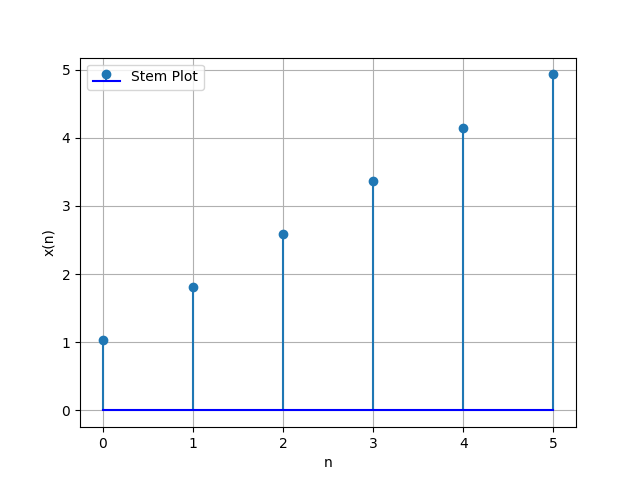
\includegraphics[width = 8cm]{figs/fig1.png}
		     \caption{Plot of $x(n) = 5 + 1.75n$}
		         \label{fig:enter-label}
 \end{figure}

\pagebreak

\end{enumerate}

\backmatter
\appendix
\chapter{ Convolution}
\input{app/conv.tex}
\chapter{ Z-transform}
\begin{enumerate}[label=\thechapter.\arabic*,ref=\thechapter.\theenumi]
\numberwithin{equation}{enumi}
\numberwithin{figure}{enumi}
\numberwithin{table}{enumi}
\item 
	The $Z$-transform of $p(n)$ is defined as
\begin{align}
P(z) = \sum_{n=-\infty}^{\infty}p(n)z^{-n}
\label{eq:ztrans}
\end{align}
\item If 
\begin{align}
	p(n) &= p_1(n)* p_2(n),
	\\
	P(z)&=P_1(z)P_2(z)
\end{align}
The above property follows from Fourier analysis and is fundamental to signal processing. 
\item For a Geometric progression defined as follows
\begin{align}
	 x\brak{n} =x\brak{0}r^nu\brak{n}
\end{align}  
\begin{align}
               X\brak{z} &= \sum_{n=-\infty}^{\infty}x\brak{n}z^{-n}\\
               &=\sum_{n=0}^{\infty}x\brak{0}r^nz^{-n}\\
                &=\sum_{n=0}^{\infty}x\brak{0}\brak{rz^{-1}}^n\\
               &= \frac{x\brak{0}}{1-rz^{-1}} & \abs{rz^{-1}}<1\\ 
               ROC &\implies \abs{z}>\abs{r} 
\end{align}
\item For a given Arithmetic progression defined as follows
\begin{align}
	x(n) &= \sbrak{x(0) + nd} u(n)\\
	X(z) &= \sum_{n = -\infty}^{\infty} x(n) z^{-n}\\ 
	&= \sum_{n = -\infty}^{\infty} \sbrak{x(0) + nd}u(n)z^{-n}\\
	&= x(0) \sum_{n = -\infty}^{\infty} u(n)z^{-n} + d \sum_{n = -\infty}^{\infty} nu(n)z^{-n}
\end{align}
Let us consider
\begin{align}
	U(z) &= \sum_{n = -\infty}^{\infty} u(n) z^{-n} = \frac{1}{1-z^{-1}}
	\qquad \qquad \text{For } \abs{z} > 1 \\
	\frac{dU(z)}{dz} &= \frac{-1}{z} \sum_{n = -\infty}^{\infty} nu(n) z^{-n}\\
	\implies z^{-1}\frac{1}{(1-z^{-1})^{2}} &= \sum_{n = -\infty}^{\infty} nu(n) z^{-n}\\
	\implies X(z) &= \frac{x(0)}{1-z^{-1}} + \frac{dz^{-1}}{(1-z^{-1})^{2}} 
	\qquad \qquad \text{For }\abs{z} > 1 
\end{align}
\end{enumerate}

\latexprintindex

\end{document}

 



\item Ramkali saved Rs 5 in the first week of a year and then increased her weekly savings by Rs 1.75. If in the $n$th week, her weekly savings become Rs 20.75, find $n$.

\solution
\iffalse
\let\negmedspace\undefined
\let\negthickspace\undefined
\documentclass[journal,12pt,twocolumn]{IEEEtran}
\usepackage{cite}
\usepackage{amsmath,amssymb,amsfonts,amsthm}
\usepackage{algorithmic}
\usepackage{graphicx}
\usepackage{textcomp}
\usepackage{xcolor}
\usepackage{txfonts}
\usepackage{listings}
\usepackage{enumitem}
\usepackage{mathtools}
\usepackage{gensymb}
\usepackage[breaklinks=true]{hyperref}
\usepackage{tkz-euclide} % loads  TikZ and tkz-base
\usepackage{listings}
\usepackage{gvv}


\newtheorem{theorem}{Theorem}[section]
\newtheorem{problem}{Problem}
\newtheorem{proposition}{Proposition}[section]
\newtheorem{lemma}{Lemma}[section]
\newtheorem{corollary}[theorem]{Corollary}
\newtheorem{example}{Example}[section]
\newtheorem{definition}[problem]{Definition}

\newcommand{\BEQA}{\begin{eqnarray}}
\newcommand{\EEQA}{\end{eqnarray}}
\newcommand{\define}{\stackrel{\triangle}{=}}
\theoremstyle{remark}
\newtheorem{rem}{Remark}

\graphicspath{./figs/}

%\bibliographystyle{ieeetr}
\begin{document}
%

\bibliographystyle{IEEEtran}


\vspace{3cm}

\title{
	%	\logo{
	Assignment-1 

	\large{EE:1205 Signals and Systems}

	Indian Institute of Technology, Hyderabad
	%	}
}
\author{Kunal Thorawade

EE23BTECH11035
}	

\maketitle


\newpage

%\tableofcontents

\bigskip
 
 \renewcommand{\thefigure}{\theenumi}
 \renewcommand{\thetable}{\theenumi}
 %\renewcommand{\theequation}{\theenumi}

 \section{\Large Question:}  Ramkali saved Rs 5 in the first week of a year and then increased her weekly savings by Rs 1.75. If in the $n$th week, her weekly savings become Rs 20.75, find $n$.

 \section{\Large Solution:} 
 \fi
 \begin{tabular}{|c|c|c|}
	\hline
	\textbf{Symbol} & \textbf{Value} & \textbf{Description} \\[6pt]
	\hline
	$x(0)$ & $25$ & first term of AP \\[6pt]
	\hline
	$d$ & $-3$ & common difference \\[6pt]
	\hline
	$x(n)$ & $(25-3n)u(n)$ & $n$-th term of AP \\[6pt]
	\hline
	$y(n)$ & $116$ & sum of terms \\[6pt]
	\hline 
\end{tabular}


 \begin{align} 
	 x(n) &= x(0) + (n)(d)
	 \\ 20.75 &= 5 + (n)(1.75)  
	 \\ \implies 15.75 &= (n)(1.75)
	 \\ \implies n &= \frac{15.75}{1.75}
	 \\ \implies n &= 9
	 \\x(n) &= 5u(n) + 1.75nu(n)
 \end{align}
 The Z-transform of a sequence $x(n)$ is given by:
 \begin{align}
	  X(z) &= \frac{5z^{-1}}{1-z^{-1}}+\frac{1.75z^{-1}}{(1-z^{-1})^{2}} ; |z| > 1
 \end{align}

 \begin{figure}
	     \centering
	         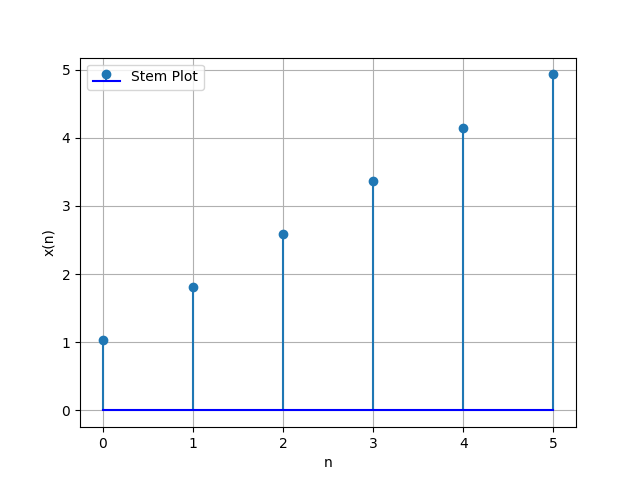
\includegraphics[width = 8cm]{figs/fig1.png}
		     \caption{Plot of $x(n) = 5 + 1.75n$}
		         \label{fig:enter-label}
 \end{figure}



\item Show that the sum of $\brak {m+n}^{th}$ and $\brak {m-n}^{th}$ terms of an $A.P.,$ is equal to twice the $m^{th}$ terms.    \\
\solution
\iffalse
\let\negmedspace\undefined
\let\negthickspace\undefined
\documentclass[journal,12pt,twocolumn]{IEEEtran}
\usepackage{cite}
\usepackage{amsmath,amssymb,amsfonts,amsthm}
\usepackage{algorithmic}
\usepackage{graphicx}
\usepackage{textcomp}
\usepackage{xcolor}
\usepackage{txfonts}
\usepackage{listings}
\usepackage{enumitem}
\usepackage{mathtools}
\usepackage{gensymb}
\usepackage{comment}
\usepackage[breaklinks=true]{hyperref}
\usepackage{tkz-euclide} 
\usepackage{listings}
\usepackage{gvv}                                        
\def\inputGnumericTable{}                                 
\usepackage[latin1]{inputenc}                                
\usepackage{color}                                            
\usepackage{array}                                            
\usepackage{longtable}                                       
\usepackage{calc}                                             
\usepackage{multirow}                                         
\usepackage{hhline}                                           
\usepackage{ifthen}                                           
\usepackage{lscape}

\newtheorem{theorem}{Theorem}[section]
\newtheorem{problem}{Problem}
\newtheorem{proposition}{Proposition}[section]
\newtheorem{lemma}{Lemma}[section]
\newtheorem{corollary}[theorem]{Corollary}
\newtheorem{example}{Example}[section]
\newtheorem{definition}[problem]{Definition}
\newcommand{\BEQA}{\begin{eqnarray}}
\newcommand{\EEQA}{\end{eqnarray}}
\newcommand{\define}{\stackrel{\triangle}{=}}
\theoremstyle{remark}
\newtheorem{rem}{Remark}
\begin{document}
\parindent 0px
\bibliographystyle{IEEEtran}
\title{Assignment 11.9.5\_1Q}
\author{EE22BTECH11219 - Rada Sai Sujan$^{}$% <-this % stops a space
}
\maketitle
\newpage
\bigskip
\section*{Question}
Show that the sum of $\brak {m+n}^{th}$ and $\brak {m-n}^{th}$ terms of an $A.P.,$ is equal to twice the $m^{th}$ terms.    \\
\solution
\fi

\begin{table}[h]
    \centering
    \def\arraystretch{1.5}
    \begin{tabular}{|c|c|c|}
    \hline
    PARAMETER & VALUE & DESCRIPTION  \\ \hline
    $$x\brak0$$ & $$x\brak{0}$$ & First term \\ \hline
    $$d$$ & $$d$$ & common difference \\ \hline
    $$x(n)$$ & $$[x\brak{0}+nd]u\brak n$$ & General term of the series  \\ \hline
  \end{tabular}

    \caption{Parameter Table1}
    \label{tab:11.9.5.1.1}
\end{table}
For an $AP$,
\begin{align}
    x\brak{n}&=[x\brak{0}+nd]u\brak{n}   \\
    \implies x\brak{m+n}+x\brak{m-n}&=[x\brak{0}+\brak{m+n}d]+[x\brak{0}+\brak{m-n}d] \\
    &=2[x\brak{0}+md]   \\
    \therefore x\brak{m+n}+x\brak{m-n}&=2x\brak{m}
\end{align}
\begin{table}[h]
    \centering
    \def\arraystretch{1.5}
    \begin{tabular}{|c|c|}
    \hline
      $$x\brak{0}$$ & $$3$$  \\ \hline
      $$d$$ & $$2$$  \\ \hline
      $$m$$ & $$6$$  \\ \hline
      $$n$$ & $$2$$  \\ \hline
      $$x\brak{m+n}$$ & $$19$$  \\ \hline
      $$x\brak{m-n}$$ & $$11$$  \\ \hline
      $$x\brak{m}$$ & $$15$$  \\ \hline
    \end{tabular}

    \caption{Verified Values}
    \label{tab:11.9.5.1.2}
\end{table}




\item The sum of the first three terms of a G.P is $39/10$ and their product is $1$. Find the common ratio and the terms.\\
\solution
\let\negmedspace\undefined
\let\negthickspace\undefined
\documentclass[journal,12pt,twocolumn]{IEEEtran}
\usepackage{cite}
\usepackage{amsmath,amssymb,amsfonts,amsthm}
\usepackage{algorithmic}
\usepackage{graphicx}
\usepackage{textcomp}
\usepackage{xcolor}
\usepackage{txfonts}
\usepackage{listings}
\usepackage{enumitem}
\usepackage{mathtools}
\usepackage{gensymb}
\usepackage{comment}
\usepackage[breaklinks=true]{hyperref}
\usepackage{tkz-euclide}
\usepackage{listings}
\usepackage{gvv}
\def\inputGnumericTable{}
\usepackage[latin1]{inputenc}
\usepackage{color}
\usepackage{array}
\usepackage{longtable}
\usepackage{calc}
\usepackage{multirow}
\usepackage{hhline}
\usepackage{ifthen}
\usepackage{lscape}

\newtheorem{theorem}{Theorem}[section]
\newtheorem{problem}{Problem}
\newtheorem{proposition}{Proposition}[section]
\newtheorem{lemma}{Lemma}[section]
\newtheorem{corollary}[theorem]{Corollary}
\newtheorem{example}{Example}[section]
\newtheorem{definition}[problem]{Definition}
\newcommand{\BEQA}{\begin{eqnarray}}
\newcommand{\EEQA}{\end{eqnarray}}
\newcommand{\define}{\stackrel{\triangle}{=}}
\theoremstyle{remark}
\newtheorem{rem}{Remark}
\begin{document}

\bibliographystyle{IEEEtran}
\vspace{3cm}

\title{NCERT Discrete - 11.9.3.12}
\author{EE23BTECH11058 - Sindam Ananya$^{*}$% <-this % stops a space
}
\maketitle
\newpage
\bigskip

\renewcommand{\thefigure}{\theenumi}
\renewcommand{\thetable}{\theenumi}

\vspace{3cm}
\textbf{Question : 11.9.3.12} 
The sum of the first three terms of a G.P is $39/10$ and their product is $1$. Find the common ratio and the terms.\\
\solution
\begin{table}[h!]
    \centering
    \begin{tabular}{|c|c|c|}
        \hline
        \textbf{Parameter} & \textbf{Value} & \textbf{Description} \\
        \hline
        $x(0)$ & & First term \\
        \hline
        $r$ & & Common ratio \\
        \hline
        $x(0)^3r^3$ & 1 & Product of terms \\
        \hline
        $x(0)$ + $x(0)r$ + $x(0)r^2$ & $\frac{39}{10}$ & Sum of terms \\
        \hline
    \end{tabular}

    \caption{Input Parameters}
    \label{tab:11.9.3.12table1}
\end{table}
\begin{equation}
y(n) = x(0)\brak{\frac{r^{n+1}-1}{r-1}}u(n)
\label{eq:11.9.3.12eq1}
\end{equation}
From \tabref{tab:11.9.3.12table1} and \eqref{eq:11.9.3.12eq1} :
\begin{align}
y(2) &= x(0)\brak{\frac{r^3-1}{r-1}}\\
\frac{39}{10} &= x(0)\brak{r^2+r+1}\\
\implies \frac{39r}{10} &= r^2+r+1 \quad \brak{\because x(0)r = 1}\\
\implies (2r-5)(5r-2) &=0\\
\implies r &= \frac{2}{5} \quad or \quad \frac{5}{2}
\end{align}
\begin{enumerate}
      \item If $r = \frac{2}{5}$, then terms are $\frac{5}{2}$, $1$, $\frac{2}{5}$.
      \item If $r = \frac{5}{2}$, then terms are $\frac{2}{5}$, $1$, $\frac{5}{2}$.
\end{enumerate}
\begin{figure}[h!]
    \centering
    \includegraphics[width=\columnwidth]{figs/graph1.png}
    \caption{stem plots of GP if $r=\frac{2}{5}$}
    \label{fig:1}
\end{figure}
\begin{figure}[h!]
    \centering
    \includegraphics[width=\columnwidth]{figs/graph2.png}
    \caption{stem plots of GP if $r=\frac{5}{2}$}
    \label{fig:1}
\end{figure}
\end{document}




\item The ratio of the A.M and G.M of two positive numbers $a$ and $b$ is $m:n$. Show that $a:b = \brak{ m + \sqrt{m^2 - n^2}} : \brak{ m - \sqrt{m^2 - n^2}}$.\\
\solution
\iffalse
\let\negmedspace\undefined
\let\negthickspace\undefined
\documentclass[journal,12pt,onecolumn]{IEEEtran}
\usepackage{cite}
\usepackage{amsmath,amssymb,amsfonts,amsthm}
\usepackage{algorithmic}
\usepackage{graphicx}
\usepackage{textcomp}
\usepackage{xcolor}
\usepackage{txfonts}
\usepackage{listings}
\usepackage{enumitem}
\usepackage{mathtools}
\usepackage{gensymb}

\usepackage{tkz-euclide} % loads  TikZ and tkz-base
\usepackage{listings}



\newtheorem{theorem}{Theorem}[section]
\newtheorem{problem}{Problem}
\newtheorem{proposition}{Proposition}[section]
\newtheorem{lemma}{Lemma}[section]
\newtheorem{corollary}[theorem]{Corollary}
\newtheorem{example}{Example}[section]
\newtheorem{definition}[problem]{Definition}
%\newtheorem{thm}{Theorem}[section] 
%\newtheorem{defn}[thm]{Definition}
%\newtheorem{algorithm}{Algorithm}[section]
%\newtheorem{cor}{Corollary}
\newcommand{\BEQA}{\begin{eqnarray}}
\newcommand{\EEQA}{\end{eqnarray}}
\newcommand{\system}[1]{\stackrel{#1}{\rightarrow}}

\newcommand{\define}{\stackrel{\triangle}{=}}
\theoremstyle{remark}
\newtheorem{rem}{Remark}
%\bibliographystyle{ieeetr}
\begin{document}
%
\providecommand{\pr}[1]{\ensuremath{\Pr\left(#1\right)}}
\providecommand{\prt}[2]{\ensuremath{p_{#1}^{\left(#2\right)} }}        % own macro for this question
\providecommand{\qfunc}[1]{\ensuremath{Q\left(#1\right)}}
\providecommand{\sbrak}[1]{\ensuremath{{}\left[#1\right]}}
\providecommand{\lsbrak}[1]{\ensuremath{{}\left[#1\right.}}
\providecommand{\rsbrak}[1]{\ensuremath{{}\left.#1\right]}}
\providecommand{\brak}[1]{\ensuremath{\left(#1\right)}}
\providecommand{\lbrak}[1]{\ensuremath{\left(#1\right.}}
\providecommand{\rbrak}[1]{\ensuremath{\left.#1\right)}}
\providecommand{\cbrak}[1]{\ensuremath{\left\{#1\right\}}}
\providecommand{\lcbrak}[1]{\ensuremath{\left\{#1\right.}}
\providecommand{\rcbrak}[1]{\ensuremath{\left.#1\right\}}}
\newcommand{\sgn}{\mathop{\mathrm{sgn}}}
\providecommand{\abs}[1]{\left\vert#1\right\vert}
\providecommand{\res}[1]{\Res\displaylimits_{#1}} 
\providecommand{\norm}[1]{\left\lVert#1\right\rVert}
%\providecommand{\norm}[1]{\lVert#1\rVert}
\providecommand{\mtx}[1]{\mathbf{#1}}
\providecommand{\mean}[1]{E\left[ #1 \right]}
\providecommand{\cond}[2]{#1\middle|#2}
\providecommand{\fourier}{\overset{\mathcal{F}}{ \rightleftharpoons}}
\newenvironment{amatrix}[1]{%
  \left(\begin{array}{@{}*{#1}{c}|c@{}}
}{%
  \end{array}\right)
}
%\providecommand{\hilbert}{\overset{\mathcal{H}}{ \rightleftharpoons}}
%\providecommand{\system}{\overset{\mathcal{H}}{ \longleftrightarrow}}
	%\newcommand{\solution}[2]{\textbf{Solution:}{#1}}
\newcommand{\solution}{\noindent \textbf{Solution: }}
\newcommand{\cosec}{\,\text{cosec}\,}
\providecommand{\dec}[2]{\ensuremath{\overset{#1}{\underset{#2}{\gtrless}}}}
\newcommand{\myvec}[1]{\ensuremath{\begin{pmatrix}#1\end{pmatrix}}}
\newcommand{\mydet}[1]{\ensuremath{\begin{vmatrix}#1\end{vmatrix}}}
\newcommand{\myaugvec}[2]{\ensuremath{\begin{amatrix}{#1}#2\end{amatrix}}}
\providecommand{\rank}{\text{rank}}
\providecommand{\pr}[1]{\ensuremath{\Pr\left(#1\right)}}
\providecommand{\qfunc}[1]{\ensuremath{Q\left(#1\right)}}
	\newcommand*{\permcomb}[4][0mu]{{{}^{#3}\mkern#1#2_{#4}}}
\newcommand*{\perm}[1][-3mu]{\permcomb[#1]{P}}
\newcommand*{\comb}[1][-1mu]{\permcomb[#1]{C}}
\providecommand{\qfunc}[1]{\ensuremath{Q\left(#1\right)}}
\providecommand{\gauss}[2]{\mathcal{N}\ensuremath{\left(#1,#2\right)}}
\providecommand{\diff}[2]{\ensuremath{\frac{d{#1}}{d{#2}}}}
\providecommand{\myceil}[1]{\left \lceil #1 \right \rceil }
\newcommand\figref{Fig.~\ref}
\newcommand\tabref{Table~\ref}
\newcommand{\sinc}{\,\text{sinc}\,}
\newcommand{\rect}{\,\text{rect}\,}
%%
%	%\newcommand{\solution}[2]{\textbf{Solution:}{#1}}
%\newcommand{\solution}{\noindent \textbf{Solution: }}
%\newcommand{\cosec}{\,\text{cosec}\,}
%\numberwithin{equation}{section}
%\numberwithin{equation}{subsection}
%\numberwithin{problem}{section}
%\numberwithin{definition}{section}
%\makeatletter
%\@addtoreset{figure}{problem}
%\makeatother

%\let\StandardTheFigure\thefigure
\let\vec\mathbf

\bibliographystyle{IEEEtran}





\bigskip

\renewcommand{\thefigure}{\theenumi}
\renewcommand{\thetable}{\theenumi}
%\renewcommand{\theequation}{\theenumi}


\title{Discrete Assignment}
\author{Karyampudi Meghana Sai\\ EE23BTECH11031}
\maketitle



The ratio of the A.M and G.M of two positive numbers $a$ and $b$ is $m:n$. Show that $a:b = \brak{ m + \sqrt{m^2 - n^2}} : \brak{ m - \sqrt{m^2 - n^2}}$.\\
\solution
\fi

Expressing A.M and G.M in terms of $a$ and $b$:
\begin{align}
\frac{a + b}{2\sqrt{ab}} = \frac{m}{n} \label{eq:11.9.5.19eq1}
\end{align}

Let's assume that $x = \sqrt{\frac{a}{b}}$. Then, we have:
\begin{align}
\frac{a}{b} = x^2 \label{eq:11.9.5.19eq2}
\end{align}

Substituting the value of x in equation \eqref{eq:11.9.5.19eq1}:
\begin{align}
\frac{1 + x^2}{2x} &= \frac{m}{n}\label{eq:11.9.5.19eq3} \\
\frac{1}{x} + x &= \frac{2m}{n} \label{eq:11.9.5.19eq4} \\
x^2 - \frac{2m}{n}x + 1 &=  0 \label{eq:11.9.5.19eq5}\\
\implies x &= \frac{m}{n} \pm \frac{\sqrt{m^2 - n^2}}{n} \label{eq:11.9.5.19eq6}
\end{align}

Since $x = \sqrt{\frac{a}{b}}$, $x$ must be positive.
\begin{align}
x = \frac{m + \sqrt{m^2 - n^2}}{n}\label{eq:11.9.5.19eq7}
\end{align}

Referencing the value of $x$ from equation\eqref{eq:11.9.5.19eq2}.
\begin{align}
\frac{a}{b} &=\brak{\frac{m + \sqrt{m^2 - n^2}}{n}}^2  \label{eq:11.9.5.19eq8}
\end{align}

Multiplying both the numerator and denominator with $\brak{m-\sqrt{m^2 - n^2}}$: 
\begin{align} 
\frac{a}{b} &= \frac{1}{n^2} \frac{\brak{m + \sqrt{m^2 - n^2}}^2  \brak{m-\sqrt{m^2 - n^2}}}{\brak{m-\sqrt{m^2 - n^2}}}\label{eq:11.9.5.19eq9}\\
\implies a:b &= \brak{ m + \sqrt{m^2 - n^2}}: \brak{m - \sqrt{m^2 - n^2}}\label{eq:11.9.5.19eq10}
\end{align}
nth term of the AP :
\begin{align}
y(n)&=\sbrak{a+n\brak{b-a}}u(n)\label{eq:11.9.5.19eq11}\\
n^k u(n) &\system{Z} (-1)^k z^k \frac{d^k}{dz^k}U(z)\label{eq:11.9.5.19eq12}\\
u(n) &\system{Z} \frac{1}{\brak{1 - z^{-1}}} \quad \abs{ z} > \abs{1} \label{eq:11.9.5.19eq13}\\
nu(n) &\system{Z} \frac{z^{-1}}{\brak{1 - z^{-1}}^2} \quad \abs{ z} > \abs{1} \label{eq:11.9.5.19eq14}
\end{align}
Referencing the equations from \eqref{eq:11.9.5.19eq13},\eqref{eq:11.9.5.19eq14}.\\
\begin{align}
y(n) &\system{Z} \frac{a}{\brak{1 - z^{-1}}}+\frac{\brak{b-a}z^{-1}}{\brak{1-z^{-1}}^2} \quad \abs{ z} > \abs{1} \label{eq:11.9.5.19eq15}
\end{align}
nth term of the GP :
\begin{align}
y(n)&=a\brak{{\frac{b}{a}}}^n u(n)\label{eq:11.9.5.19eq16}\\
r^n u(n) &\system{Z} \frac{1}{\brak{1-rz^{-1}}} \quad \abs{ z} > \abs{r} \label{eq:11.9.5.19eq17}
\end{align}
Referencing the equation from \eqref{eq:11.9.5.19eq17}.\\
\begin{align}
y(n) &\system{Z} \frac{a^2 z^{-1}}{\brak{a-bz^{-1}}} \quad \abs{ z} > \abs{\frac{b}{a}}\label{eq:11.9.5.19eq18}
\end{align}
%\end{document}



\item The sum of three numbers in an arithmetic progression (AP) is $24$ and the product of those three numbers is $440$, find the values of the three numbers.\\
\solution
\iffalse
\documentclass[12pt]{article}
\usepackage{amsmath , amssymb}
\usepackage{graphicx}
\usepackage{float}
\usepackage{pgfplots}
\pgfplotsset{compat=1.18}
\newcommand{\tabref}[1]{Table~\ref{#1}}
\newcommand{\figref}[1]{Figure~\ref{#1}}
\providecommand{\abs}[1]{\left\vert#1\right\vert}

\begin{document}

\title{Discrete Assignment}
\author{Mohana Eppala\\ EE23BTECH11018}
\maketitle

\section*{Problem Statement}
Find the value of $n$ so that $\frac{a^{n+1} + b^{n+1}}{a^{n}+b^{n}}$ may be the geometric mean between $a$ and $b$.
\section*{Solution}
\fi
\begin{table}[H]
\centering
\begin{tabular}{|c|c|c|}
        \hline
        \textbf{Parameter} & \textbf{Value} & \textbf{Description} \\
        \hline
	$x(0)$ & $a$ & First term \\
        \hline
	$x(2)$ & $b$ & Third term \\
	\hline
	$x(1)$ & $\sqrt{ab}=\frac{a^{n+1}+b^{n+1}}{a^{n}+b^{n}}$ & Second term\\
	\hline
	$r$ & $\sqrt{\frac{b}{a}}$ & Common ratio \\
	\hline
        $n$ & - & Given variable \\
        \hline
	$x(k)$ & $ar^{k}u(k)$ & General term \\
	\hline
\end{tabular}
\caption{Input parameters table}
\label{tab:11.9.3.27.1}

\end{table}

Consider a GP as in \tabref{tab:1},
\begin{align}
	\therefore \frac{a^{n+1} + b^{n+1}}{a^{n}+b^{n}} &= x(1) \\
	\implies a^{n+1} + b^{n+1} &= a^{n+\frac{1}{2}}b^{\frac{1}{2}} + a^{\frac{1}{2}}b^{n+\frac{1}{2}} \\
\implies a^{n+\frac{1}{2}}(a^{\frac{1}{2}} - b^{\frac{1}{2}}) &= b^{n+\frac{1}{2}}(a^{\frac{1}{2}} - b^{\frac{1}{2}}) \\
\implies (\frac{a}{b})^{n+\frac{1}{2}} &= (\frac{a}{b})^{0} \\
\implies n &= -\frac{1}{2}
\end{align}
From \tabref{tab:1},
\begin{align}
	X(z) &= \frac{a}{1-(\sqrt{\frac{b}{a}})z^{-1}} \quad \abs{z}>\abs{\sqrt{\frac{b}{a}}}
\end{align}
%\end{document}

\pagebreak

\item The sum of some terms of G.P. is $315$ whose first term and the common ratio are $5$ and $2$ , respectively. Find the last term and the number of terms.\\
\solution
\iffalse
\let\negmedspace\undefined
\let\negthickspace\undefined
\documentclass[journal,12pt,twocolumn]{IEEEtran}
\usepackage{cite}
\usepackage{amsmath,amssymb,amsfonts,amsthm}
\usepackage{algorithmic}
\usepackage{graphicx}
\usepackage{textcomp}
\usepackage{xcolor}
\usepackage{txfonts}
\usepackage{listings}
\usepackage{enumitem}
\usepackage{mathtools}
\usepackage{gensymb}
\usepackage{comment}
\usepackage[breaklinks=true]{hyperref}
\usepackage{tkz-euclide}
\usepackage{listings}
\usepackage{gvv}
\def\inputGnumericTable{}
\usepackage[latin1]{inputenc}
\usepackage{color}
\usepackage{array}
\usepackage{longtable}
\usepackage{calc}
\usepackage{multirow}
\usepackage{hhline}
\usepackage{ifthen}
\usepackage{lscape}

\newtheorem{theorem}{Theorem}[section]
\newtheorem{problem}{Problem}
\newtheorem{proposition}{Proposition}[section]
\newtheorem{lemma}{Lemma}[section]
\newtheorem{corollary}[theorem]{Corollary}
\newtheorem{example}{Example}[section]
\newtheorem{definition}[problem]{Definition}
\newcommand{\BEQA}{\begin{eqnarray}}
\newcommand{\EEQA}{\end{eqnarray}}
\newcommand{\define}{\stackrel{\triangle}{=}}
\theoremstyle{remark}
\newtheorem{rem}{Remark}
\begin{document}

\bibliographystyle{IEEEtran}
\vspace{3cm}

\title{NCERT Discrete - 10.5.3.20}
\author{EE23BTECH1205 - Avani Chouhan$^{*}$% <-this % stops a space
}
\maketitle
\newpage
\bigskip

\renewcommand{\thefigure}{\theenumi}
\renewcommand{\thetable}{\theenumi}

\vspace{3cm}
\textbf{Question : 10.5.3.20} 
The sum of some terms of G.P. is 315 whose first term and the common ratio are $5$ and $2$ , respectively. Find the last term and the number of terms.\\
\solution
\fi
\begin{table}
  \centering
  \begin{tabular}{|c|c|c|}
    \hline
    \textbf{Parameter} & \textbf{Value} & \textbf{Description} \\
    \hline
    $x(0)$ & $5$ & First term \\
    \hline
    $r$ & $2$ & Common ratio \\
    \hline
    $y(n)$ & $315$ & Sum of $n+1$ terms \\
    \hline
    $x(n)$ & ? & Last term\\
    \hline
\end{tabular}


  \caption{Input Parameters}
  \label{tab:10.5.3.20table1}
\end{table}
\begin{align}
x(n) = x(0)r^{n}u(n)
\label{eq:10.5.3.20eq}
\end{align}
From \eqref{eq:gpz}
\begin{align}
X(z) =\frac{5}{1-2z^{-1}} \quad \abs{z} > \abs{2}
\end{align}
By contour integration:
\begin{align}
y(n) &= x(0)\brak{\frac{r^{n+1}-1}{r-1}}u(n)\\
315 &= 5\brak{2^{n+1}- 1}  \\
\implies n &= 5
\end{align}
The number of terms is \(n + 1 = 6\)\\
From \eqref{eq:10.5.3.20eq}:
\begin{align}
x(5) &= 5\brak{2^{5}}\\
 &= 160 
\end{align}

\begin{figure}[H]
    \centering
    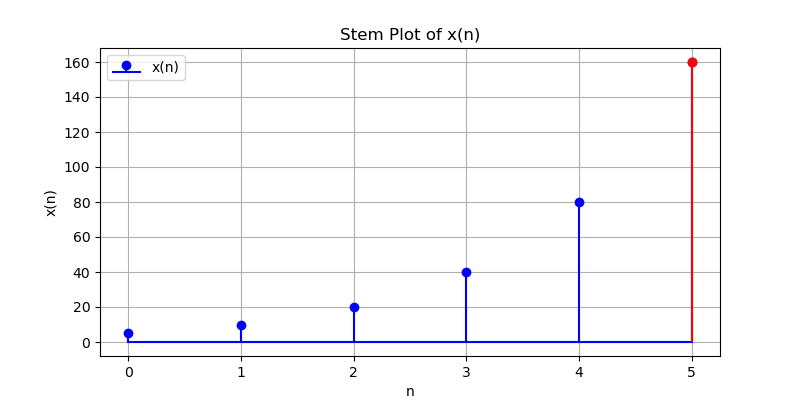
\includegraphics[width=\columnwidth]{ncert-maths/11/9/5/8/figs/plot1.png}
    \caption{Stem plot of x(n)}
    \label{fig:10.5.3.20fig1}
\end{figure}
\begin{figure}[H]
    \centering
    \includegraphics[width=\columnwidth]{ncert-maths/11/9/5/8/figs/plot2.png}
    \caption{Stem plot of y(n)}
    \label{fig:10.5.3.20fig2}
\end{figure}
%\end{document}

\pagebreak

\item  Find the sum of n terms of the A.P. whose kth term is \(5k + 1\).\\
\solution
\iffalse
\documentclass[journal,12pt,twocolumn]{IEEEtran}
\usepackage{cite}
\usepackage{amsmath,amssymb,amsfonts,amsthm}
\usepackage{algorithmic}
\usepackage{graphicx}
\usepackage{textcomp}
\usepackage{xcolor}
\usepackage{txfonts}
\usepackage{listings}
\usepackage{enumitem}
\usepackage{mathtools}
\usepackage{gensymb}
\usepackage{comment}
\usepackage[breaklinks=true]{hyperref}
\usepackage{tkz-euclide} 
\usepackage{textgreek}                       
\usepackage{circuitikz}
\usepackage{pgfplots}                            
\usepackage[latin1]{inputenc}                                
\usepackage{color}                                            
\usepackage{array}                                            
\usepackage{longtable}                                       
\usepackage{calc}                                             
\usepackage{multirow}                                         
\usepackage{hhline}                                           
\usepackage{ifthen}                                           
\usepackage{lscape}


\newtheorem{theorem}{Theorem}[section]
\newtheorem{problem}{Problem}
\newtheorem{proposition}{Proposition}[section]
\newtheorem{lemma}{Lemma}[section]
\newtheorem{corollary}[theorem]{Corollary}
\newtheorem{example}{Example}[section]
\newtheorem{definition}[problem]{Definition}
\newcommand{\BEQA}{\begin{eqnarray}}
\newcommand{\EEQA}{\end{eqnarray}}
\newcommand{\define}{\stackrel{\triangle}{=}}
\theoremstyle{remark}
\newtheorem{rem}{Remark}

\begin{document}
\providecommand{\brak}[1]{\ensuremath{\left(#1\right)}}
\bibliographystyle{IEEEtran}
\vspace{3cm}

\title{NCERT 11.9.2 Q7}
\author{EE23BTECH11204 - Ashley Ann Benoy$^{*}$}% <-this % stops a space
\maketitle
\newpage
\bigskip
\bibliographystyle{IEEEtran}
\textbf{Question: Find the sum of n terms of the A.P. whose kth term is \(5k + 1\).}\\
\solution
\fi
\begin{table}[h!]
    \centering
    \resizebox{6cm}{!}{
        
\begin{tabular}{|c|c|c|}
\hline
\textbf{Symbol} & \textbf{Value} & \textbf{Parameter} \\
\hline
\(x(0)\) & \(1 \) & First Term \\
\hline
\(x(n)\) & \((5n+1)u(n)\) & kth Term \\
\hline
\(d\) & \(5 \) & Common Difference \\
\hline
\end{tabular}


    }
    \\
    \caption{Given Parameters}
    \label{tab:ash_params}  
\end{table}

Apply the Z-transform to \( x\brak{n} \):
\begin{align}
X\brak{z} = \frac{5z^{-1}}{\brak{1 - z^{-1}}^2} + \frac{1}{\brak{1 - z^{-1}}}
\quad |z|>1
\end{align}

Sum of First \( n \) Terms:

\begin{align}
y\brak{n} = x\brak{n} * u\brak{n}
\end{align}

Applying Z transform on both sides:
\begin{align}
    Y\brak{z} &= X\brak{z}U\brak{z}
\end{align}

\begin{align}
&=\frac{1}{\brak{1 - z^{-1}}^2} + \frac{5}{2} \cdot \frac{2z^{-1}}{\brak{1 - z^{-1}}^3} 
\end{align}
\\
Now we can compare the  above pairs as;
\begin{align}
nu\brak{n} \xleftrightarrow{\text{Z}} \frac{z^{-1}}{(1 - z^{-1})^2}
\end{align}
\begin{align}
u\brak{n} \xleftrightarrow{\text{Z}} \frac{1}{(1 - z^{-1})}
\end{align}
\begin{align}
n\brak{n-1}u\brak{n} \xleftrightarrow{\text{Z}} \frac{2z^{-1}}{(1 - z^{-1})^3}
\end{align}
On referring the above equations and comparing, we can obtain the  Z transform inverse as follows:

\begin{align}
y\brak{n} = \brak{n+1 }u\brak{n} + \frac{5}{2} n\brak{n-1} u\brak{n}
\end{align}
\begin{align}
&= \brak{n+1 + \frac{5}{2} n\brak{n-1}}u\brak{n}
\end{align}
Since we are taking n starting from 0 we replace n with n+1 to make our simulation match with the theory\\Therefore, we have got the sum of n terms as:\\
\begin{align}
y\brak{n}= \brak{n+2 + \frac{5}{2} n\brak{n+1}}u\brak{n+1}
\end{align}
The stem plot is given as
\begin{figure}[h!]
  \centering
  \includegraphics[width=\columnwidth]{ncert-maths/11/9/2/7/figs/Figure_1.png}
  \label{fig:Spash}
\end{figure}
%\end{document}


\pagebreak

\item How many 3 digit numbers are divisible by 7? \\
\solution

\item A person writes a letter to four of his friends. He asks each one of them to copy the letter and mail to four different persons with instruction that they move the chain similarly. Assuming that the chain is not broken and that it costs 50 paise to mail one letter. Find the amount spent on the postage when 8th set of letter is mailed.\\
\solution 
\pagebreak

\item If $a$, $b$, $c$ are in A.P.; $b$, $c$, $d$ are in G.P and $\frac{1}{c}$, $\frac{1}{d}$, $\frac{1}{e}$ are in A.P. prove that $a$, $c$, $e$ are in G.P.\\
\solution
\pagebreak
\item Find the 31st term of an AP whose $11$th term is 38 and the $16$th term is 73.\\ 
\solution
%% Run LaTeX on this file several times to get Table of Contents,
%% cross-references, and citations.
\documentclass[11pt]{book}
\usepackage{gvv-book}
\usepackage{gvv}
%\usepackage{Wiley-AuthoringTemplate}
\usepackage[sectionbib,authoryear]{natbib}% for name-date citation comment the below line
%\usepackage[sectionbib,numbers]{natbib}% for numbered citation comment the above line

%%********************************************************************%%
%%       How many levels of section head would you like numbered?     %%
%% 0= no section numbers, 1= section, 2= subsection, 3= subsubsection %%
\setcounter{secnumdepth}{3}
%%********************************************************************%%
%%**********************************************************************%%
%%     How many levels of section head would you like to appear in the  %%
%%				Table of Contents?			%%
%% 0= chapter, 1= section, 2= subsection, 3= subsubsection titles.	%%
\setcounter{tocdepth}{2}
%%**********************************************************************%%

%\includeonly{ch01}
\makeindex

\begin{document}

\frontmatter
%%%%%%%%%%%%%%%%%%%%%%%%%%%%%%%%%%%%%%%%%%%%%%%%%%%%%%%%%%%%%%%%
%% Title Pages
%% Wiley will provide title and copyright page, but you can make
%% your own titlepages if you'd like anyway
%% Setting up title pages, type in the appropriate names here:

\booktitle{Signal Processing \\ Fundamentals}

\subtitle{Through NCERT}

\AuAff{G. V. V. Sharma}


%% \\ will start a new line.
%% You may add \affil{} for affiliation, ie,
%\authors{Robert M. Groves\\
%\affil{Universitat de les Illes Balears}
%Floyd J. Fowler, Jr.\\
%\affil{University of New Mexico}
%}

%% Print Half Title and Title Page:
%\halftitlepage
\titlepage

%%%%%%%%%%%%%%%%%%%%%%%%%%%%%%%%%%%%%%%%%%%%%%%%%%%%%%%%%%%%%%%%
%% Copyright Page

\begin{copyrightpage}{2024}
%Title, etc
\end{copyrightpage}

% Note, you must use \ to start indented lines, ie,
% 
% \begin{copyrightpage}{2004}
% Survey Methodology / Robert M. Groves . . . [et al.].
% \       p. cm.---(Wiley series in survey methodology)
% \    ``Wiley-Interscience."
% \    Includes bibliographical references and index.
% \    ISBN 0-471-48348-6 (pbk.)
% \    1. Surveys---Methodology.  2. Social 
% \  sciences---Research---Statistical methods.  I. Groves, Robert M.  II. %
% Series.\\

% HA31.2.S873 2004
% 001.4'33---dc22                                             2004044064
% \end{copyrightpage}

%%%%%%%%%%%%%%%%%%%%%%%%%%%%%%%%%%%%%%%%%%%%%%%%%%%%%%%%%%%%%%%%
%% Only Dedication (optional) 

%\dedication{To my parents}

\tableofcontents

%\listoffigures %optional
%\listoftables  %optional

%% or Contributor Page for edited books
%% before \tableofcontents

%%%%%%%%%%%%%%%%%%%%%%%%%%%%%%%%%%%%%%%%%%%%%%%%%%%%%%%%%%%%%%%%
%  Contributors Page for Edited Book
%%%%%%%%%%%%%%%%%%%%%%%%%%%%%%%%%%%%%%%%%%%%%%%%%%%%%%%%%%%%%%%%

% If your book has chapters written by different authors,
% you'll need a Contributors page.

% Use \begin{contributors}...\end{contributors} and
% then enter each author with the \name{} command, followed
% by the affiliation information.

% \begin{contributors}
% \name{Masayki Abe,} Fujitsu Laboratories Ltd., Fujitsu Limited, Atsugi, Japan
%
% \name{L. A. Akers,} Center for Solid State Electronics Research, Arizona State University, Tempe, Arizona
%
% \name{G. H. Bernstein,} Department of Electrical and Computer Engineering, University of Notre Dame, Notre Dame, South Bend, Indiana; formerly of
% Center for Solid State Electronics Research, Arizona
% State University, Tempe, Arizona 
% \end{contributors}

%%%%%%%%%%%%%%%%%%%%%%%%%%%%%%%%%%%%%%%%%%%%%%%%%%%%%%%%%%%%%%%%
% Optional Foreword:

%\begin{foreword}
%\lipsum[1-2]
%\end{foreword}

%%%%%%%%%%%%%%%%%%%%%%%%%%%%%%%%%%%%%%%%%%%%%%%%%%%%%%%%%%%%%%%%
% Optional Preface:

%\begin{preface}
%\lipsum[1-1]
%\prefaceauthor{}
%\where{place\\
% date}
%\end{preface}

% ie,
% \begin{preface}
% This is an example preface.
% \prefaceauthor{R. K. Watts}
% \where{Durham, North Carolina\\
% September, 2004}

%%%%%%%%%%%%%%%%%%%%%%%%%%%%%%%%%%%%%%%%%%%%%%%%%%%%%%%%%%%%%%%%
% Optional Acknowledgments:

%\acknowledgments
%\lipsum[1-2]
%\authorinitials{I. R. S.}  

%%%%%%%%%%%%%%%%%%%%%%%%%%%%%%%%
%% Glossary Type of Environment:

% \begin{glossary}
% \term{<term>}{<description>}
% \end{glossary}

%%%%%%%%%%%%%%%%%%%%%%%%%%%%%%%%
%\begin{acronyms}
%\acro{ASTA}{Arrivals See Time Averages}
%\acro{BHCA}{Busy Hour Call Attempts}
%\acro{BR}{Bandwidth Reservation}
%\acro{b.u.}{bandwidth unit(s)}
%\acro{CAC}{Call / Connection Admission Control}
%\acro{CBP}{Call Blocking Probability(-ies)}
%\acro{CCS}{Centum Call Seconds}
%\acro{CDTM}{Connection Dependent Threshold Model}
%\acro{CS}{Complete Sharing}
%\acro{DiffServ}{Differentiated Services}
%\acro{EMLM}{Erlang Multirate Loss Model}
%\acro{erl}{The Erlang unit of traffic-load}
%\acro{FIFO}{First in - First out}
%\acro{GB}{Global balance}
%\acro{GoS}{Grade of Service}
%\acro{ICT}{Information and Communication Technology}
%\acro{IntServ}{Integrated Services}
%\acro{IP}{Internet Protocol}
%\acro{ITU-T}{International Telecommunication Unit -- Standardization sector}
%\acro{LB}{Local balance}
%\acro{LHS}{Left hand side}
%\acro{LIFO}{Last in - First out}
%\acro{MMPP}{Markov Modulated Poisson Process}
%\acro{MPLS}{Multiple Protocol Labeling Switching}
%\acro{MRM}{Multi-Retry Model}
%\acro{MTM}{Multi-Threshold Model}
%\acro{PASTA}{Poisson Arrivals See Time Averages}
%\acro{PDF}{Probability Distribution Function}
%\acro{pdf}{probability density function}
%\acro{PFS}{Product Form Solution}
%\acro{QoS}{Quality of Service}
%\acro{r.v.}{random variable(s)}
%\acro{RED}{random early detection}
%\acro{RHS}{Right hand side}
%\acro{RLA}{Reduced Load Approximation}
%\acro{SIRO}{service in random order}
%\acro{SRM}{Single-Retry Model}
%\acro{STM}{Single-Threshold Model}
%\acro{TCP}{Transport Control Protocol}
%\acro{TH}{Threshold(s)}
%\acro{UDP}{User Datagram Protocol}
%\end{acronyms}

\setcounter{page}{1}

\begin{introduction}
This book introduces some concepts in signal processing through maths and physics problems in
NCERT textbooks.

\end{introduction}

\mainmatter

\chapter{Analog}
\section{Harmonics}
\begin{enumerate}[label=\thesection.\arabic*,ref=\thesection.\theenumi]
\item A circular disk of mass 10kg is suspended by a wire attached to its centre. The wire is twisted by rotating the disc and released. The period of torsional oscillations is found to be 1.5s. The radius of the disc is 15cm. Determine the torsional spring constant of the wire. (Torsional spring constant $\alpha$ is defined by the relation J=-$\alpha$$\theta$, where J is the restoring couple and $\theta$ is the angle of twist).\\
\solution
\pagebreak
\item Suppose that the electric field amplitude of an electromagnetic wave is $E_0$ = 120N/C and that its frequency is $f$ = 50.0 MHz.
\begin{enumerate} [label=(\alph*)]
    \item Determine, $B_0, \omega, k$ and $\lambda$
    \item Find expressions for \textbf{E} and \textbf{B}
\end{enumerate}
\solution
%% Run LaTeX on this file several times to get Table of Contents,
%% cross-references, and citations.
\documentclass[11pt]{book}
\usepackage{gvv-book}
\usepackage{gvv}
%\usepackage{Wiley-AuthoringTemplate}
\usepackage[sectionbib,authoryear]{natbib}% for name-date citation comment the below line
%\usepackage[sectionbib,numbers]{natbib}% for numbered citation comment the above line

%%********************************************************************%%
%%       How many levels of section head would you like numbered?     %%
%% 0= no section numbers, 1= section, 2= subsection, 3= subsubsection %%
\setcounter{secnumdepth}{3}
%%********************************************************************%%
%%**********************************************************************%%
%%     How many levels of section head would you like to appear in the  %%
%%				Table of Contents?			%%
%% 0= chapter, 1= section, 2= subsection, 3= subsubsection titles.	%%
\setcounter{tocdepth}{2}
%%**********************************************************************%%

%\includeonly{ch01}
\makeindex

\begin{document}

\frontmatter
%%%%%%%%%%%%%%%%%%%%%%%%%%%%%%%%%%%%%%%%%%%%%%%%%%%%%%%%%%%%%%%%
%% Title Pages
%% Wiley will provide title and copyright page, but you can make
%% your own titlepages if you'd like anyway
%% Setting up title pages, type in the appropriate names here:

\booktitle{Signal Processing \\ Fundamentals}

\subtitle{Through NCERT}

\AuAff{G. V. V. Sharma}


%% \\ will start a new line.
%% You may add \affil{} for affiliation, ie,
%\authors{Robert M. Groves\\
%\affil{Universitat de les Illes Balears}
%Floyd J. Fowler, Jr.\\
%\affil{University of New Mexico}
%}

%% Print Half Title and Title Page:
%\halftitlepage
\titlepage

%%%%%%%%%%%%%%%%%%%%%%%%%%%%%%%%%%%%%%%%%%%%%%%%%%%%%%%%%%%%%%%%
%% Copyright Page

\begin{copyrightpage}{2024}
%Title, etc
\end{copyrightpage}

% Note, you must use \ to start indented lines, ie,
% 
% \begin{copyrightpage}{2004}
% Survey Methodology / Robert M. Groves . . . [et al.].
% \       p. cm.---(Wiley series in survey methodology)
% \    ``Wiley-Interscience."
% \    Includes bibliographical references and index.
% \    ISBN 0-471-48348-6 (pbk.)
% \    1. Surveys---Methodology.  2. Social 
% \  sciences---Research---Statistical methods.  I. Groves, Robert M.  II. %
% Series.\\

% HA31.2.S873 2004
% 001.4'33---dc22                                             2004044064
% \end{copyrightpage}

%%%%%%%%%%%%%%%%%%%%%%%%%%%%%%%%%%%%%%%%%%%%%%%%%%%%%%%%%%%%%%%%
%% Only Dedication (optional) 

%\dedication{To my parents}

\tableofcontents

%\listoffigures %optional
%\listoftables  %optional

%% or Contributor Page for edited books
%% before \tableofcontents

%%%%%%%%%%%%%%%%%%%%%%%%%%%%%%%%%%%%%%%%%%%%%%%%%%%%%%%%%%%%%%%%
%  Contributors Page for Edited Book
%%%%%%%%%%%%%%%%%%%%%%%%%%%%%%%%%%%%%%%%%%%%%%%%%%%%%%%%%%%%%%%%

% If your book has chapters written by different authors,
% you'll need a Contributors page.

% Use \begin{contributors}...\end{contributors} and
% then enter each author with the \name{} command, followed
% by the affiliation information.

% \begin{contributors}
% \name{Masayki Abe,} Fujitsu Laboratories Ltd., Fujitsu Limited, Atsugi, Japan
%
% \name{L. A. Akers,} Center for Solid State Electronics Research, Arizona State University, Tempe, Arizona
%
% \name{G. H. Bernstein,} Department of Electrical and Computer Engineering, University of Notre Dame, Notre Dame, South Bend, Indiana; formerly of
% Center for Solid State Electronics Research, Arizona
% State University, Tempe, Arizona 
% \end{contributors}

%%%%%%%%%%%%%%%%%%%%%%%%%%%%%%%%%%%%%%%%%%%%%%%%%%%%%%%%%%%%%%%%
% Optional Foreword:

%\begin{foreword}
%\lipsum[1-2]
%\end{foreword}

%%%%%%%%%%%%%%%%%%%%%%%%%%%%%%%%%%%%%%%%%%%%%%%%%%%%%%%%%%%%%%%%
% Optional Preface:

%\begin{preface}
%\lipsum[1-1]
%\prefaceauthor{}
%\where{place\\
% date}
%\end{preface}

% ie,
% \begin{preface}
% This is an example preface.
% \prefaceauthor{R. K. Watts}
% \where{Durham, North Carolina\\
% September, 2004}

%%%%%%%%%%%%%%%%%%%%%%%%%%%%%%%%%%%%%%%%%%%%%%%%%%%%%%%%%%%%%%%%
% Optional Acknowledgments:

%\acknowledgments
%\lipsum[1-2]
%\authorinitials{I. R. S.}  

%%%%%%%%%%%%%%%%%%%%%%%%%%%%%%%%
%% Glossary Type of Environment:

% \begin{glossary}
% \term{<term>}{<description>}
% \end{glossary}

%%%%%%%%%%%%%%%%%%%%%%%%%%%%%%%%
%\begin{acronyms}
%\acro{ASTA}{Arrivals See Time Averages}
%\acro{BHCA}{Busy Hour Call Attempts}
%\acro{BR}{Bandwidth Reservation}
%\acro{b.u.}{bandwidth unit(s)}
%\acro{CAC}{Call / Connection Admission Control}
%\acro{CBP}{Call Blocking Probability(-ies)}
%\acro{CCS}{Centum Call Seconds}
%\acro{CDTM}{Connection Dependent Threshold Model}
%\acro{CS}{Complete Sharing}
%\acro{DiffServ}{Differentiated Services}
%\acro{EMLM}{Erlang Multirate Loss Model}
%\acro{erl}{The Erlang unit of traffic-load}
%\acro{FIFO}{First in - First out}
%\acro{GB}{Global balance}
%\acro{GoS}{Grade of Service}
%\acro{ICT}{Information and Communication Technology}
%\acro{IntServ}{Integrated Services}
%\acro{IP}{Internet Protocol}
%\acro{ITU-T}{International Telecommunication Unit -- Standardization sector}
%\acro{LB}{Local balance}
%\acro{LHS}{Left hand side}
%\acro{LIFO}{Last in - First out}
%\acro{MMPP}{Markov Modulated Poisson Process}
%\acro{MPLS}{Multiple Protocol Labeling Switching}
%\acro{MRM}{Multi-Retry Model}
%\acro{MTM}{Multi-Threshold Model}
%\acro{PASTA}{Poisson Arrivals See Time Averages}
%\acro{PDF}{Probability Distribution Function}
%\acro{pdf}{probability density function}
%\acro{PFS}{Product Form Solution}
%\acro{QoS}{Quality of Service}
%\acro{r.v.}{random variable(s)}
%\acro{RED}{random early detection}
%\acro{RHS}{Right hand side}
%\acro{RLA}{Reduced Load Approximation}
%\acro{SIRO}{service in random order}
%\acro{SRM}{Single-Retry Model}
%\acro{STM}{Single-Threshold Model}
%\acro{TCP}{Transport Control Protocol}
%\acro{TH}{Threshold(s)}
%\acro{UDP}{User Datagram Protocol}
%\end{acronyms}

\setcounter{page}{1}

\begin{introduction}
This book introduces some concepts in signal processing through maths and physics problems in
NCERT textbooks.

\end{introduction}

\mainmatter

\chapter{Analog}
\section{Harmonics}
\input{ncert-physics/analog.tex}
\section{Filters}
\input{ncert-physics/analog-filters.tex}
\chapter{Discrete}
\section{ Z-transform}
\input{ncert-maths/z-transform}
\section{Sequences}
\input{ncert-maths/sequences}
\backmatter
\appendix
\chapter{ Convolution}
\input{app/conv.tex}
\chapter{ Z-transform}
\input{app/mgf.tex}
\latexprintindex

\end{document}

 


\pagebreak
\item A charged particle oscillates about its mean equilibrium position with a frequency of $10^9Hz$. What is the frequency of the electromagnetic waves produced by the oscillator? \\
\solution

\iffalse
\documentclass[journal,12pt,twocolumn]{IEEEtran}
\usepackage{cite}
\usepackage{amsmath,amssymb,amsfonts,amsthm}
\usepackage{algorithmic}
\usepackage{graphicx}
\usepackage{textcomp}
\usepackage{xcolor}
\usepackage{txfonts}
\usepackage{listings}
\usepackage{enumitem}
\usepackage{mathtools}
\usepackage{float}
\usepackage{gensymb}
\usepackage{comment}
\usepackage[breaklinks=true]{hyperref}
\usepackage{tkz-euclide} 
\usepackage{listings}
\usepackage{gvv}                                        
\def\inputGnumericTable{}                                 
\usepackage[latin1]{inputenc}                                
\usepackage{color}                                            
\usepackage{array}                                            
\usepackage{longtable}                                       
\usepackage{calc}                                             
\usepackage{multirow}                                         
\usepackage{hhline}                                           
\usepackage{ifthen}                                           
\usepackage{lscape}
\usepackage{amsmath}
\newtheorem{theorem}{Theorem}[section]
\newtheorem{problem}{Problem}
\newtheorem{proposition}{Proposition}[section]
\newtheorem{lemma}{Lemma}[section]
\newtheorem{corollary}[theorem]{Corollary}
\newtheorem{example}{Example}[section]
\newtheorem{definition}[problem]{Definition}
\newcommand{\BEQA}{\begin{eqnarray}}
\newcommand{\EEQA}{\end{eqnarray}}
\newcommand{\define}{\stackrel{\triangle}{=}}
\theoremstyle{remark}
\newtheorem{rem}{Remark}

\begin{document}

\bibliographystyle{IEEEtran}
\vspace{3cm}

\title{NCERT Discrete - 11.9.1.8}
\author{EE23BTECH11045 - Palavelli Srija$^{*}$}

\maketitle
\newpage
\bigskip

\renewcommand{\thefigure}{\theenumi}
\renewcommand{\thetable}{\theenumi}

\vspace{3cm}
\textbf{Question 11.9.1.8:} 
\begin{enumerate}
\item Find the seventh term of the sequence where the nth term is given by $a_n= \frac {n^2}{2^{n}}$
\end{enumerate}

\textbf{Solution: }
\fi
\begin{align}
 x(n) &= \frac{(n+1)^2}{2^{(n+1)}}u(n)
\end{align}

\begin{table}[h!]
    \centering
    \input{ncert-maths/11/9/1/11.9.1.8/tables/table1.tex}
    \caption{Input Parameters}
    \label{tab:table_9.8.1}
\end{table}

\begin{align}
x(6) &= \frac{(6+1)^2}{2^{(6+1)}}\\
     &= \frac {49}{128}
\end{align}

\begin{enumerate}
   \item Scaling property:
     \begin{align}
         a^{n} u(n) & \xleftrightarrow{\mathcal{Z}}  \frac{1}{(1-az^{-1})}, \quad \lvert z \rvert > \lvert a \rvert 
     \end{align}
     
   \item Differentiation property:
    \begin{align}
     n u(n) & \xleftrightarrow{\mathcal{Z}} (-z) \frac{dY(z)}{dz} \\
     \implies n u(n) & \xleftrightarrow{\mathcal{Z}}  \frac{z^{-1}}{(1-z^{-1})^2}, \quad \lvert z \rvert > 1 \\
     \implies n^2 u(n) & \xleftrightarrow{\mathcal{Z}}  \frac{z^{-1}(1+z^{-1})}{(1-z^{-1})^3}, \quad \lvert z \rvert > 1
   \end{align}
   
   \item Time shifting property:
    \begin{align}
         y(n-k) & \xleftrightarrow{\mathcal{Z}} z^{-k}Y(z)
     \end{align}
\end{enumerate}

The Z transform of $x(n)$ is given by:\\
from(4)
\begin{align}
\frac{u(n)}{2^n} & \xleftrightarrow{\mathcal{Z}}  \frac{1}{(1-(2z)^{-1})}, \quad \lvert z \rvert>\frac{1}{2}
\end{align}
	from(5)
\begin{align}
\frac{n}{2^n} u(n) & \xleftrightarrow{\mathcal{Z}} \frac{(2z)^{-1}}{(1-(2z)^{-1})^2}, \quad \lvert z \rvert>\frac{1}{2}\\
\frac{n^2}{2^n} u(n) & \xleftrightarrow{\mathcal{Z}} \frac{(2z)^{-1}(1 + (2z)^{-1})}{(1 - (2z)^{-1})^3}, \quad \lvert z \rvert>\frac{1}{2}
\end{align}
	from(8)
\begin{align}
\frac{(n+1)^2}{2^(n+1)} u(n) & \xleftrightarrow{\mathcal{Z}} (z) \frac{(2z)^{-1}(1 + (2z)^{-1})}{(1 - (2z)^{-1})^3}, \quad \lvert z \rvert > \frac{1}{2}
\end{align}

\begin{align}
X(z) &= \frac{1 + (2z)^{-1}}{2(1 - (2z)^{-1})^3}, \quad \lvert z \rvert > \frac{1}{2}
\end{align}

\begin{figure}[h!]
    \centering
    \includegraphics[width=\columnwidth]{ncert-maths/11/9/1/11.9.1.8/figs/plot.png}
    \caption{Stem plot of $x(n)$}
    \label{fig:1}
\end{figure}

%\end{document}

\pagebreak
\item Given below are some functions of x and t to 
represent the displacement (transverse
or longitudinal) of an elastic wave. State which of these represents \brak i travelling
wave, \brak {ii} a stationary wave or \brak {iii} none at all: \\
\begin{enumerate}
\item $y = 2\cos \brak{3x} \sin \brak{10t}$
\item $y=2\sqrt{x-vt}$
\item $y = 3\sin \brak{5x - 0.5t} + 4\cos \brak{5x - 0.5t}$
\item $y = \cos x \sin t + \cos 2x \sin 2t$
\end{enumerate}
\solution
\iffalse
\let\negmedspace\undefined
\let\negthickspace\undefined
\documentclass[journal,12pt,twocolumn]{IEEEtran}
\usepackage{cite}
\usepackage{amsmath,amssymb,amsfonts,amsthm}
\usepackage{algorithmic}
\usepackage{graphicx}
\usepackage{textcomp}
\usepackage{xcolor}
\usepackage{txfonts}
\usepackage{listings}
\usepackage{enumitem}
\usepackage{mathtools}
\usepackage{gensymb}
\usepackage{comment}
\usepackage[breaklinks=true]{hyperref}
\usepackage{tkz-euclide} 
\usepackage{listings}
\usepackage{gvv}                                        
\def\inputGnumericTable{}                                 
\usepackage[latin1]{inputenc}                                
\usepackage{color}                                            
\usepackage{array}                                            
\usepackage{longtable}                                       
\usepackage{calc}                                             
\usepackage{multirow}                                         
\usepackage{hhline}                                           
\usepackage{ifthen}                                           
\usepackage{lscape}
\newtheorem{theorem}{Theorem}[section]
\newtheorem{problem}{Problem}
\newtheorem{proposition}{Proposition}[section]
\newtheorem{lemma}{Lemma}[section]
\newtheorem{corollary}[theorem]{Corollary}
\newtheorem{example}{Example}[section]
\newtheorem{definition}[problem]{Definition}
\newcommand{\BEQA}{\begin{eqnarray}}
\newcommand{\EEQA}{\end{eqnarray}}
\newcommand{\define}{\stackrel{\triangle}{=}}
\theoremstyle{remark}
\newtheorem{rem}{Remark}
\begin{document}
\parindent 0px
\bibliographystyle{IEEEtran}
\title{ASSIGNMENT11.15\_13Q}
\author{EE22BTECH11219 - Sai Sujan Rada$^{}$% <-this % stops a space
}
\maketitle
\newpage
\bigskip
\section*{QUESTION}
Given below are some functions of x and t to 
represent the displacement (transverse
or longitudinal) of an elastic wave. State which of these represents \brak i travelling
wave, \brak {ii} a stationary wave or \brak {iii} none at all: \\
\begin{enumerate}
\item $y = 2\cos \brak{3x} \sin \brak{10t}$
\item $y=2\sqrt{x-vt}$
\item $y = 3\sin \brak{5x - 0.5t} + 4\cos \brak{5x - 0.5t}$
\item $y = \cos x \sin t + \cos 2x \sin 2t$
\end{enumerate}
\solution 
\fi

\input{ncert-physics/11/15/13/tables/TABLE1.tex}
Let us assume an equation:
\begin{align}
y=A(x)\cos \brak{\omega t+\phi\brak {x}}
\end{align}
\input{ncert-physics/11/15/13/tables/TABLE2.tex}
\begin{figure}[h]
                        \centering
                        \includegraphics[width=\columnwidth]{ncert-physics/11/15/13/figs/a.png}
                        \caption{DIPLACEMENT $vs$ TIME-graph1}
                        \label{fig:11.13.1}
\end{figure}
\begin{figure}[h]
                            \centering
                            \includegraphics[width=\columnwidth]{ncert-physics/11/15/13/figs/b.png}
                            \caption{DIPLACEMENT $vs$ TIME-graph2}
                            \label{fig:11.13.2}
\end{figure}   
\begin{figure}[h]
                             \centering
                             \includegraphics[width=\columnwidth]{ncert-physics/11/15/13/figs/c.png}
                             \caption{DIPLACEMENT $vs$ TIME-graph3}
                             \label{fig:11.13.3}
\end{figure}
\begin{figure}[h]
                            \centering
                            \includegraphics[width=\columnwidth]{ncert-physics/11/15/13/figs/d.png}
                            \caption{DIPLACEMENT $vs$ TIME-graph4}
                            \label{fig:11.13.4}
\end{figure}
\figref{fig:11.13.1} and \figref{fig:11.13.3} are self explanatory for stationary and travelling waves.
\figref{fig:11.13.2} and \figref{fig:11.13.4} are neither stationary nor travelling waves. 


\pagebreak
\item For the travelling harmonic wave
$y\brak {x, t} = 2.0 \cos 2\pi \brak{10t - 0.0080 x + 0.35}$ where $x$ and $y$ are in $cm$ and $t$ in $s$. Calculate the phase difference between oscillatory
motion of two points separated by a distance of 

\begin{enumerate} [label=(\alph*)]
    \item $4 m$
    \item $0.5 m$
    \item $\lambda/2$
    \item $3\lambda/4$
\end{enumerate}
\solution
\iffalse
\let\negmedspace\undefined
\let\negthickspace\undefined
\documentclass[journal,12pt,twocolumn]{IEEEtran}
\usepackage{cite}
\usepackage{amsmath,amssymb,amsfonts,amsthm}
\usepackage{algorithmic}
\usepackage{graphicx}
\usepackage{textcomp}
\usepackage{xcolor}
\usepackage{txfonts}
\usepackage{listings}
\usepackage{enumitem}
\usepackage{mathtools}
\usepackage{gensymb}
\usepackage{comment}
\usepackage[breaklinks=true]{hyperref}
\usepackage{tkz-euclide} 
\usepackage{listings}
\usepackage{gvv}                                        
\def\inputGnumericTable{}                                 
\usepackage[latin1]{inputenc}                               \usepackage{caption}
\usepackage{color}                                            
\usepackage{array}                                            
\usepackage{longtable}                                       
\usepackage{calc}                                             
\usepackage{multirow}                                         
\usepackage{hhline}                                           
\usepackage{ifthen}                                           
\usepackage{lscape}

\newtheorem{theorem}{Theorem}[section]
\newtheorem{problem}{Problem}
\newtheorem{proposition}{Proposition}[section]
\newtheorem{lemma}{Lemma}[section]
\newtheorem{corollary}[theorem]{Corollary}
\newtheorem{example}{Example}[section]
\newtheorem{definition}[problem]{Definition}
\newcommand{\BEQA}{\begin{eqnarray}}
\newcommand{\EEQA}{\end{eqnarray}}
\newcommand{\define}{\stackrel{\triangle}{=}}
\theoremstyle{remark}
\newtheorem{rem}{Remark}
\begin{document}

\bibliographystyle{IEEEtran}
\vspace{3cm}

\title{NCERT 11.15. Q10}
\author{EE23BTECH11010 - Venkatesh Bandawar$^{*}$% <-this % stops a space
}
\maketitle
\newpage
\bigskip

\renewcommand{\thefigure}{\arabic{figure}}
\renewcommand{\thetable}{\arabic{table}}

\bibliographystyle{IEEEtran}

\parindent 0px
\textbf{Question:} For the travelling harmonic wave
$y\brak {x, t} = 2.0 \cos 2\pi \brak{10t - 0.0080 x + 0.35}$ where $x$ and $y$ are in $cm$ and $t$ in $s$. Calculate the phase difference between oscillatory
motion of two points separated by a distance of 

\begin{enumerate} [label=(\alph*)]
    \item $4 m$
    \item $0.5 m$
    \item $\lambda/2$
    \item $3\lambda/4$
\end{enumerate}

\solution
\fi
\begin{table}[htbp] \small
\centering
\input{ncert-physics/11/15/10/tables/table1.tex}
\caption{Given \, parameters list}
\label{tab:11.15.10.1}
\end{table}
\begin{align}
    \brak{\Delta \theta} &= \brak{ 2\pi f t - kx_1 + \phi}  - \brak{2\pi f t -kx_2 + \phi}\\
    &= k\brak{x_2 - x_1} 
\end{align}

\begin{table}[htbp] 
\centering
\input{ncert-physics/11/15/10/tables/table2.tex}
\caption{Phase \, differences}
\label{tab:11.15.10.2}
\end{table}

\begin{figure}[!h] 
\centering
\includegraphics[width=\columnwidth]{ncert-physics/11/15/10/figs/graph1.png}
\captionsetup{justification=centering}
\caption{}
\label{fig:11.15.10.1}
\end{figure}

\begin{figure}[!h] 
\centering
\includegraphics[width=\columnwidth]{ncert-physics/11/15/10/figs/graph2.png}
\captionsetup{justification=centering}
\caption{}
\label{fig:11.15.10.2}
\end{figure}

\begin{figure}[!h] 
\centering
\includegraphics[width=\columnwidth]{ncert-physics/11/15/10/figs/graph3.png}
\captionsetup{justification=centering}
\caption{}
\label{fig:11.15.10.3}
\end{figure}

\begin{figure}[!h] 
\centering
\includegraphics[width=\columnwidth]{ncert-physics/11/15/10/figs/graph4.png}
\captionsetup{justification=centering}
\caption{}
\label{fig:11.15.10.4}
\end{figure}


\pagebreak
\item 
\begin{enumerate}
\item The peak voltage of an AC supply is 300 V. What is the rms voltage?
\item The rms value of current in an AC circuit is 10 A. What is the peak current?
\end{enumerate}
\solution
%% Run LaTeX on this file several times to get Table of Contents,
%% cross-references, and citations.
\documentclass[11pt]{book}
\usepackage{gvv-book}
\usepackage{gvv}
%\usepackage{Wiley-AuthoringTemplate}
\usepackage[sectionbib,authoryear]{natbib}% for name-date citation comment the below line
%\usepackage[sectionbib,numbers]{natbib}% for numbered citation comment the above line

%%********************************************************************%%
%%       How many levels of section head would you like numbered?     %%
%% 0= no section numbers, 1= section, 2= subsection, 3= subsubsection %%
\setcounter{secnumdepth}{3}
%%********************************************************************%%
%%**********************************************************************%%
%%     How many levels of section head would you like to appear in the  %%
%%				Table of Contents?			%%
%% 0= chapter, 1= section, 2= subsection, 3= subsubsection titles.	%%
\setcounter{tocdepth}{2}
%%**********************************************************************%%

%\includeonly{ch01}
\makeindex

\begin{document}

\frontmatter
%%%%%%%%%%%%%%%%%%%%%%%%%%%%%%%%%%%%%%%%%%%%%%%%%%%%%%%%%%%%%%%%
%% Title Pages
%% Wiley will provide title and copyright page, but you can make
%% your own titlepages if you'd like anyway
%% Setting up title pages, type in the appropriate names here:

\booktitle{Signal Processing \\ Fundamentals}

\subtitle{Through NCERT}

\AuAff{G. V. V. Sharma}


%% \\ will start a new line.
%% You may add \affil{} for affiliation, ie,
%\authors{Robert M. Groves\\
%\affil{Universitat de les Illes Balears}
%Floyd J. Fowler, Jr.\\
%\affil{University of New Mexico}
%}

%% Print Half Title and Title Page:
%\halftitlepage
\titlepage

%%%%%%%%%%%%%%%%%%%%%%%%%%%%%%%%%%%%%%%%%%%%%%%%%%%%%%%%%%%%%%%%
%% Copyright Page

\begin{copyrightpage}{2024}
%Title, etc
\end{copyrightpage}

% Note, you must use \ to start indented lines, ie,
% 
% \begin{copyrightpage}{2004}
% Survey Methodology / Robert M. Groves . . . [et al.].
% \       p. cm.---(Wiley series in survey methodology)
% \    ``Wiley-Interscience."
% \    Includes bibliographical references and index.
% \    ISBN 0-471-48348-6 (pbk.)
% \    1. Surveys---Methodology.  2. Social 
% \  sciences---Research---Statistical methods.  I. Groves, Robert M.  II. %
% Series.\\

% HA31.2.S873 2004
% 001.4'33---dc22                                             2004044064
% \end{copyrightpage}

%%%%%%%%%%%%%%%%%%%%%%%%%%%%%%%%%%%%%%%%%%%%%%%%%%%%%%%%%%%%%%%%
%% Only Dedication (optional) 

%\dedication{To my parents}

\tableofcontents

%\listoffigures %optional
%\listoftables  %optional

%% or Contributor Page for edited books
%% before \tableofcontents

%%%%%%%%%%%%%%%%%%%%%%%%%%%%%%%%%%%%%%%%%%%%%%%%%%%%%%%%%%%%%%%%
%  Contributors Page for Edited Book
%%%%%%%%%%%%%%%%%%%%%%%%%%%%%%%%%%%%%%%%%%%%%%%%%%%%%%%%%%%%%%%%

% If your book has chapters written by different authors,
% you'll need a Contributors page.

% Use \begin{contributors}...\end{contributors} and
% then enter each author with the \name{} command, followed
% by the affiliation information.

% \begin{contributors}
% \name{Masayki Abe,} Fujitsu Laboratories Ltd., Fujitsu Limited, Atsugi, Japan
%
% \name{L. A. Akers,} Center for Solid State Electronics Research, Arizona State University, Tempe, Arizona
%
% \name{G. H. Bernstein,} Department of Electrical and Computer Engineering, University of Notre Dame, Notre Dame, South Bend, Indiana; formerly of
% Center for Solid State Electronics Research, Arizona
% State University, Tempe, Arizona 
% \end{contributors}

%%%%%%%%%%%%%%%%%%%%%%%%%%%%%%%%%%%%%%%%%%%%%%%%%%%%%%%%%%%%%%%%
% Optional Foreword:

%\begin{foreword}
%\lipsum[1-2]
%\end{foreword}

%%%%%%%%%%%%%%%%%%%%%%%%%%%%%%%%%%%%%%%%%%%%%%%%%%%%%%%%%%%%%%%%
% Optional Preface:

%\begin{preface}
%\lipsum[1-1]
%\prefaceauthor{}
%\where{place\\
% date}
%\end{preface}

% ie,
% \begin{preface}
% This is an example preface.
% \prefaceauthor{R. K. Watts}
% \where{Durham, North Carolina\\
% September, 2004}

%%%%%%%%%%%%%%%%%%%%%%%%%%%%%%%%%%%%%%%%%%%%%%%%%%%%%%%%%%%%%%%%
% Optional Acknowledgments:

%\acknowledgments
%\lipsum[1-2]
%\authorinitials{I. R. S.}  

%%%%%%%%%%%%%%%%%%%%%%%%%%%%%%%%
%% Glossary Type of Environment:

% \begin{glossary}
% \term{<term>}{<description>}
% \end{glossary}

%%%%%%%%%%%%%%%%%%%%%%%%%%%%%%%%
%\begin{acronyms}
%\acro{ASTA}{Arrivals See Time Averages}
%\acro{BHCA}{Busy Hour Call Attempts}
%\acro{BR}{Bandwidth Reservation}
%\acro{b.u.}{bandwidth unit(s)}
%\acro{CAC}{Call / Connection Admission Control}
%\acro{CBP}{Call Blocking Probability(-ies)}
%\acro{CCS}{Centum Call Seconds}
%\acro{CDTM}{Connection Dependent Threshold Model}
%\acro{CS}{Complete Sharing}
%\acro{DiffServ}{Differentiated Services}
%\acro{EMLM}{Erlang Multirate Loss Model}
%\acro{erl}{The Erlang unit of traffic-load}
%\acro{FIFO}{First in - First out}
%\acro{GB}{Global balance}
%\acro{GoS}{Grade of Service}
%\acro{ICT}{Information and Communication Technology}
%\acro{IntServ}{Integrated Services}
%\acro{IP}{Internet Protocol}
%\acro{ITU-T}{International Telecommunication Unit -- Standardization sector}
%\acro{LB}{Local balance}
%\acro{LHS}{Left hand side}
%\acro{LIFO}{Last in - First out}
%\acro{MMPP}{Markov Modulated Poisson Process}
%\acro{MPLS}{Multiple Protocol Labeling Switching}
%\acro{MRM}{Multi-Retry Model}
%\acro{MTM}{Multi-Threshold Model}
%\acro{PASTA}{Poisson Arrivals See Time Averages}
%\acro{PDF}{Probability Distribution Function}
%\acro{pdf}{probability density function}
%\acro{PFS}{Product Form Solution}
%\acro{QoS}{Quality of Service}
%\acro{r.v.}{random variable(s)}
%\acro{RED}{random early detection}
%\acro{RHS}{Right hand side}
%\acro{RLA}{Reduced Load Approximation}
%\acro{SIRO}{service in random order}
%\acro{SRM}{Single-Retry Model}
%\acro{STM}{Single-Threshold Model}
%\acro{TCP}{Transport Control Protocol}
%\acro{TH}{Threshold(s)}
%\acro{UDP}{User Datagram Protocol}
%\end{acronyms}

\setcounter{page}{1}

\begin{introduction}
This book introduces some concepts in signal processing through maths and physics problems in
NCERT textbooks.

\end{introduction}

\mainmatter

\chapter{Analog}
\section{Harmonics}
\input{ncert-physics/analog.tex}
\section{Filters}
\input{ncert-physics/analog-filters.tex}
\chapter{Discrete}
\section{ Z-transform}
\input{ncert-maths/z-transform}
\section{Sequences}
\input{ncert-maths/sequences}
\backmatter
\appendix
\chapter{ Convolution}
\input{app/conv.tex}
\chapter{ Z-transform}
\input{app/mgf.tex}
\latexprintindex

\end{document}

 


\pagebreak
\item In Young’s double-slit experiment using monochromatic light of wavelength $\lambda$, the intensity of light at a point on the screen where path difference is $\lambda$, is $K$ units. What is the intensity of light at a
point where path difference is $\lambda$/3?\\

\solution

%% Run LaTeX on this file several times to get Table of Contents,
%% cross-references, and citations.
\documentclass[11pt]{book}
\usepackage{gvv-book}
\usepackage{gvv}
%\usepackage{Wiley-AuthoringTemplate}
\usepackage[sectionbib,authoryear]{natbib}% for name-date citation comment the below line
%\usepackage[sectionbib,numbers]{natbib}% for numbered citation comment the above line

%%********************************************************************%%
%%       How many levels of section head would you like numbered?     %%
%% 0= no section numbers, 1= section, 2= subsection, 3= subsubsection %%
\setcounter{secnumdepth}{3}
%%********************************************************************%%
%%**********************************************************************%%
%%     How many levels of section head would you like to appear in the  %%
%%				Table of Contents?			%%
%% 0= chapter, 1= section, 2= subsection, 3= subsubsection titles.	%%
\setcounter{tocdepth}{2}
%%**********************************************************************%%

%\includeonly{ch01}
\makeindex

\begin{document}

\frontmatter
%%%%%%%%%%%%%%%%%%%%%%%%%%%%%%%%%%%%%%%%%%%%%%%%%%%%%%%%%%%%%%%%
%% Title Pages
%% Wiley will provide title and copyright page, but you can make
%% your own titlepages if you'd like anyway
%% Setting up title pages, type in the appropriate names here:

\booktitle{Signal Processing \\ Fundamentals}

\subtitle{Through NCERT}

\AuAff{G. V. V. Sharma}


%% \\ will start a new line.
%% You may add \affil{} for affiliation, ie,
%\authors{Robert M. Groves\\
%\affil{Universitat de les Illes Balears}
%Floyd J. Fowler, Jr.\\
%\affil{University of New Mexico}
%}

%% Print Half Title and Title Page:
%\halftitlepage
\titlepage

%%%%%%%%%%%%%%%%%%%%%%%%%%%%%%%%%%%%%%%%%%%%%%%%%%%%%%%%%%%%%%%%
%% Copyright Page

\begin{copyrightpage}{2024}
%Title, etc
\end{copyrightpage}

% Note, you must use \ to start indented lines, ie,
% 
% \begin{copyrightpage}{2004}
% Survey Methodology / Robert M. Groves . . . [et al.].
% \       p. cm.---(Wiley series in survey methodology)
% \    ``Wiley-Interscience."
% \    Includes bibliographical references and index.
% \    ISBN 0-471-48348-6 (pbk.)
% \    1. Surveys---Methodology.  2. Social 
% \  sciences---Research---Statistical methods.  I. Groves, Robert M.  II. %
% Series.\\

% HA31.2.S873 2004
% 001.4'33---dc22                                             2004044064
% \end{copyrightpage}

%%%%%%%%%%%%%%%%%%%%%%%%%%%%%%%%%%%%%%%%%%%%%%%%%%%%%%%%%%%%%%%%
%% Only Dedication (optional) 

%\dedication{To my parents}

\tableofcontents

%\listoffigures %optional
%\listoftables  %optional

%% or Contributor Page for edited books
%% before \tableofcontents

%%%%%%%%%%%%%%%%%%%%%%%%%%%%%%%%%%%%%%%%%%%%%%%%%%%%%%%%%%%%%%%%
%  Contributors Page for Edited Book
%%%%%%%%%%%%%%%%%%%%%%%%%%%%%%%%%%%%%%%%%%%%%%%%%%%%%%%%%%%%%%%%

% If your book has chapters written by different authors,
% you'll need a Contributors page.

% Use \begin{contributors}...\end{contributors} and
% then enter each author with the \name{} command, followed
% by the affiliation information.

% \begin{contributors}
% \name{Masayki Abe,} Fujitsu Laboratories Ltd., Fujitsu Limited, Atsugi, Japan
%
% \name{L. A. Akers,} Center for Solid State Electronics Research, Arizona State University, Tempe, Arizona
%
% \name{G. H. Bernstein,} Department of Electrical and Computer Engineering, University of Notre Dame, Notre Dame, South Bend, Indiana; formerly of
% Center for Solid State Electronics Research, Arizona
% State University, Tempe, Arizona 
% \end{contributors}

%%%%%%%%%%%%%%%%%%%%%%%%%%%%%%%%%%%%%%%%%%%%%%%%%%%%%%%%%%%%%%%%
% Optional Foreword:

%\begin{foreword}
%\lipsum[1-2]
%\end{foreword}

%%%%%%%%%%%%%%%%%%%%%%%%%%%%%%%%%%%%%%%%%%%%%%%%%%%%%%%%%%%%%%%%
% Optional Preface:

%\begin{preface}
%\lipsum[1-1]
%\prefaceauthor{}
%\where{place\\
% date}
%\end{preface}

% ie,
% \begin{preface}
% This is an example preface.
% \prefaceauthor{R. K. Watts}
% \where{Durham, North Carolina\\
% September, 2004}

%%%%%%%%%%%%%%%%%%%%%%%%%%%%%%%%%%%%%%%%%%%%%%%%%%%%%%%%%%%%%%%%
% Optional Acknowledgments:

%\acknowledgments
%\lipsum[1-2]
%\authorinitials{I. R. S.}  

%%%%%%%%%%%%%%%%%%%%%%%%%%%%%%%%
%% Glossary Type of Environment:

% \begin{glossary}
% \term{<term>}{<description>}
% \end{glossary}

%%%%%%%%%%%%%%%%%%%%%%%%%%%%%%%%
%\begin{acronyms}
%\acro{ASTA}{Arrivals See Time Averages}
%\acro{BHCA}{Busy Hour Call Attempts}
%\acro{BR}{Bandwidth Reservation}
%\acro{b.u.}{bandwidth unit(s)}
%\acro{CAC}{Call / Connection Admission Control}
%\acro{CBP}{Call Blocking Probability(-ies)}
%\acro{CCS}{Centum Call Seconds}
%\acro{CDTM}{Connection Dependent Threshold Model}
%\acro{CS}{Complete Sharing}
%\acro{DiffServ}{Differentiated Services}
%\acro{EMLM}{Erlang Multirate Loss Model}
%\acro{erl}{The Erlang unit of traffic-load}
%\acro{FIFO}{First in - First out}
%\acro{GB}{Global balance}
%\acro{GoS}{Grade of Service}
%\acro{ICT}{Information and Communication Technology}
%\acro{IntServ}{Integrated Services}
%\acro{IP}{Internet Protocol}
%\acro{ITU-T}{International Telecommunication Unit -- Standardization sector}
%\acro{LB}{Local balance}
%\acro{LHS}{Left hand side}
%\acro{LIFO}{Last in - First out}
%\acro{MMPP}{Markov Modulated Poisson Process}
%\acro{MPLS}{Multiple Protocol Labeling Switching}
%\acro{MRM}{Multi-Retry Model}
%\acro{MTM}{Multi-Threshold Model}
%\acro{PASTA}{Poisson Arrivals See Time Averages}
%\acro{PDF}{Probability Distribution Function}
%\acro{pdf}{probability density function}
%\acro{PFS}{Product Form Solution}
%\acro{QoS}{Quality of Service}
%\acro{r.v.}{random variable(s)}
%\acro{RED}{random early detection}
%\acro{RHS}{Right hand side}
%\acro{RLA}{Reduced Load Approximation}
%\acro{SIRO}{service in random order}
%\acro{SRM}{Single-Retry Model}
%\acro{STM}{Single-Threshold Model}
%\acro{TCP}{Transport Control Protocol}
%\acro{TH}{Threshold(s)}
%\acro{UDP}{User Datagram Protocol}
%\end{acronyms}

\setcounter{page}{1}

\begin{introduction}
This book introduces some concepts in signal processing through maths and physics problems in
NCERT textbooks.

\end{introduction}

\mainmatter

\chapter{Analog}
\section{Harmonics}
\input{ncert-physics/analog.tex}
\section{Filters}
\input{ncert-physics/analog-filters.tex}
\chapter{Discrete}
\section{ Z-transform}
\input{ncert-maths/z-transform}
\section{Sequences}
\input{ncert-maths/sequences}
\backmatter
\appendix
\chapter{ Convolution}
\input{app/conv.tex}
\chapter{ Z-transform}
\input{app/mgf.tex}
\latexprintindex

\end{document}

 

\pagebreak

\item In a plane electromagnetic wave, the electric field oscillates sinusoidally at a frequency of $2.0 \text{ x } 10^{10}$ Hz and amplitude 48 $Vm^{-1}$.
\begin{enumerate}[label=(\alph*)]
    \item What is the wavelength of the wave?
    \item What is the amplitude of the oscillating magnetic field?
    \item Show that the average energy density of the $\vec{E}$ field equals the
average energy density of the $\vec{B}$ field. $[c = 3 \text{ x } 10^{8}ms^{-1} ]$
\end{enumerate}

\item \begin{enumerate}
\item For the wave on the string $y(x, t) = 0.06 \sin(\frac{2\pi x}{3}) \cos(120\pi t)$ , do all the points on the string     oscillate with the same (a)frequency , (b)phase , (c)amplitude ? Explain your answers. \\

 \item What is the amplitude of a point 0.375m away from one end? \\
 \end{enumerate}
 \solution
 \pagebreak
 
 \item 
 A transverse harmonic wave on a string is described by
\begin{align}
    y\brak{x,t}=3.0 \sin\brak{36t+0.018x+\frac{\pi}{4}}
\end{align}
where $x$ and $y$ are in cm and $t$ in s. The positive direction of $x$ is from left to right.
\begin{enumerate}[label=(\alph*)]
    \item Is this a travelling wave or a stationary wave? If it is travelling, what are the speed and direction of its propogation?
    \item What are its amplitude and frequency?
    \item What is the initial phase at the origin?
    \item  What is the least distance between two succesive crests in the wave?
\end{enumerate}

\solution
\pagebreak

\item In deriving the single slit diffraction pattern, it was stated that the intensity is zero at angles of $\frac{n\lambda}{a}$. Justify this by suitably dividing the slit to bring out the cancellation.\\
\solution
\pagebreak

\item A 60 $\mu$ F capacitor is connected to a 110 V, 60 Hz ac supply. Determine the rms value of the current in the circuit.\\
\solution
\pagebreak

\item A charged  $30\mu F$ capacitor is connected to a $27 mH$ inductor. What is the angular frequency of free oscillations of the circuit?\\
\solution
\pagebreak
\item Obtain the resonance frequency of a series LCR circuit with $L = 2.0\, H$, $C = 32\, \mu F$, and $R = 10\, \Omega$. What is the Q-value of the circuit.\\
\solution
\pagebreak
\item A charged 30 $\mu$F capacitor is connected to a 27 mH inductor. Suppose the initial charge on the capacitor is 6mC.What is the total energy stored in the circuit initially? What is the
total energy at later time? \\
\solution
\pagebreak

\item A wire stretched between two rigid supports vibrates in its fundamental mode with a frequency of $45 \, \text{Hz}$. The mass of the wire is $3.5 \times 10^{-2} \, \text{kg}$, and its linear mass density is $4.0 \times 10^{-2} \, \text{kg/m}$. The length of the wire is $0.875 \, \text{m}$. Determine the speed of a transverse wave on the string and the tension in the string.\\
\solution
\pagebreak

\item The given figure shows a series LCR circuit connected to a variable
frequency 230 V source. \\
L = 5.0 H, C = 80 $\mu$F, R = 40 $\Omega$.

\begin{figure}[h!]
\begin{center}
\begin{circuitikz}[american voltages]
      \draw (0,0)
      to[sV, l=$\varepsilon$] (0,2) 
      to[R, l=$R$, v=$V_R$] (4,2) 
      to[C, l=$C$, v=$V_C$] (4,0)
      to[L, l=$L$, v=$V_L$] (0,0);
\end{circuitikz}
\end{center}
\end{figure}

\begin{enumerate}
    \item Determine the source frequency which drives the circuit in resonance.
    \item Obtain the impedance of the circuit and the amplitude of current
at the resonating frequency.
    \item Determine the rms potential drops across the three elements of
the circuit. Show that the potential drop across the LC
combination is zero at the resonating frequency.\\
\end{enumerate}
\solution
\pagebreak

\item Q23) A narrow sound pulse (for example, a short pip by a whistle) is sent across a
	medium.\\ \brak{\text{a}} Does the pulse have a definite \brak{\text{i}} frequency, \brak{\text{ii}} wavelength, \brak{\text{iii}} speed
	of propagation?\\[1ex]\brak{\text{b}} If the pulse rate is 1 after every 20 s, (that is the whistle is
	blown for a split of second after every 20 s), Is the frequency of note produced
	by whistle equal to 1/20 or 0.05 Hz ?\\
\solution
\pagebreak
\item Suppose that the electric field part of an electromagnetic wave in vacuum given as\\ \textbf{E} =\{(3.1N/C)cos[(1.8 rad/m)y+(5.4$\times$10$^{6}$rad/s)t]\}\^i \\
(a) What is the direction of propagation ?\\
(b) What is the wavelength ? \\
(c) What is the frequency ?\\
(d) What is the amplitude of the magnetic field part of the wave?\\
(e) Write an expression for the magnetic field part of the wave.\\
\solution
\pagebreak

\item A 44 mH inductor is connected to 220 V, 50 Hz ac supply. Determine
the rms value of the current in the circuit.\\
\solution
\pagebreak

\item The 6563 \AA\, H$\alpha$ line emitted by hydrogen in a star is found to be redshifted by 15 \AA. Estimate the speed with which the star is receding from the Earth.
\solution
\pagebreak
\item The amplitude  of the magnetic part of a harmonic elctromagnetic wave is $B_0=510$nT.What is the amplitude of the electric part of the electromagnetic wave.\\
\solution
\pagebreak

\item A 100$\mu$F capacitor in series with a 40$\Omega$ resistance is connected to a 110V, 60Hz supply.
\begin{enumerate}[label = {\brak{\alph*}}]
\item What is the maximum current in the circuit?
\item What is the time lag between the current maximum and the voltage maximum?\\
\end{enumerate}
\solution
\pagebreak
\item A 100 $\ohm$ resistor is connected to $220 V$, $50 Hz$ AC supply.\\
(1) What is the rms value of current in the circuit?\\
(2) What is the net power consumed over a full cycle?

\solution
\pagebreak
\item  Two towers on top of two hills are $40$ km apart.This line joining them passes $50$ m above a hill halfway between the towers.What is the longest wavelength of radio waves,which can be sent between the towers without  appereciable diffraction effects?\\
\solution
\pagebreak
\item A circuit containing a 80mH inductor and a 60$\mu$F capacitor in series is connected to a 230V, 50Hz supply. The resistance of the circuit is negligible.\\
\begin{enumerate}
  \item Obtain the current amplitude and rms value.
  \item Obtain the rms value of potential drops across each element.
  \item What is the average power transferred to the inductor ?
  \item What is the average power transferred to the capacitor ?
  \item What is the total average power absorbed by the circuit ? \brak{\text{'Average' implies 'averaged over one cycle'.}}
\end{enumerate}
\solution
\pagebreak
\item A coil of inductance 0.50 H and resistance 100 $\Omega$ is connected to a 240 V, 50 Hz ac supply.\\
(a) What is the maximum current in the coil?\\		
(b) What is the time lag between the voltage maximum and the current maximum?\\
\solution
\pagebreak

\item A plane electromagnetic wave travels in vacuum along the \(z\)-direction. What can you say about the directions of its electric (\(\mathbf{E}\)) and magnetic (\(\mathbf{B}\)) field vectors? If the frequency of the wave is \(30 \, \text{MHz}\), what can you say about its wavelength?\\
\solution
\pagebreak

\item
Earthquakes generate sound waves inside the earth. Unlike a gas, the earth can experience both transverse (S) and longitudinal (P) sound waves. Typically the speed of S wave is about $4.0 km/s$, and that of P wave is $8.0 km/s$. A seismograph records P and S waves from an earthquake. The first P wave arrives $4 min$ before the first S wave. Assuming the waves travel in straight line, at what distance does the
earthquake occur ?
\solution
\pagebreak

\item
A hospital uses an ultrasonic scanner to locate tumors in a tissue. What is the wavelength of sound in the tissue in which the speed of sound is $1.7 \, \text{km/s}$? The operating frequency of the scanner is $4.2 \, \text{MHz}$.
\solution
\pagebreak

\item In double-slit experiment using light of wavelength $600 nm$, the
angular width of a fringe formed on a distant screen is $0.1\degree$. What is
the spacing between the two slits?\\
\solution
\pagebreak

\item Figures correspond to two circular motions. The radius of the circle, the period of revolution, the initial position and the sense of revolution(i.e. clockwise or anti-clockwise) are indicated on each figure. Obtain the corresponding simple harmonic motions of the x-projections of the radius vector of resolving particle P in each case.

\begin{figure}[h]
        \centering
        \includegraphics[width=0.5\columnwidth]{ncert-physics/11/14/11/codes/qfig.pdf}
\end{figure}
\solution
\pagebreak



\end{enumerate}

\section{Filters}
\begin{enumerate}[label=\thesection.\arabic*,ref=\thesection.\theenumi]
\item An LC circuit contains a $50 \mu H$ inductor and a $50 \mu F$ capacitor with an initial charge of $10 mC$. The resistance of the circuit is negligible. Let the instant the circuit is closed by $t = 0$.

\textbf{a)} What is the total energy stored initially? Is it conserved during LC oscillations?

\textbf{b)} What is the natural frequency of the circuit?

\textbf{c)} At what time is the energy stored \textbf{(i)} completely electrical (i.e., stored in the capacitor)? \textbf{(ii)} completely magnetic (i.e., stored in the inductor)?

\textbf{d)} At what times is the total energy shared equally between the inductor and the capacitor?

\textbf{e)} If a resistor is inserted in the circuit, how much energy is eventually dissipated as heat? \\
\hfill(NCERT-Physics 12.7 12Q)\\
\solution 
\pagebreak 

\item Obtain the resonant frequency and Q-factor of a series LCR circuit with $L = 3.0\, H$, $C = 27\, \mu F$, and $R = 7.4\, \Omega$. It is desired to improve the sharpness of the resonance of the circuit by reducing its `full width at half maximum' by a factor of 2. Suggest a suitable way.\\
\solution
\input{ncert-physics/12/7/21/Phy_12_7_21.tex}

\pagebreak
\item A circuit containing a $80 mH$ inductor and a $60 \mu F$ capacitor in series is connected to a $230 V$, $50 Hz$ supply. A resistance of $15 \Omega $ is connected in series. Obtain the average power transferred to each element of the circuit, and the total power absorbed.\\
\solution
\pagebreak

\item A series LCR circuit with 
$L$ = $0.12 H$
$C$ = $480 nF$
$R$ = $23 \Omega$
is connected to a $230 V$ variable frequency supply.\\
(a) What is the source frequency for which current amplitude is maximum? Obtain this maximum value.\\
(b) What is the source frequency for which the average power absorbed by the circuit is maximum? Obtain the value of this maximum power.\\
(c) For which frequencies of the source is the power transferred to the circuit half the power at resonant frequency? What is the current amplitude at these frequencies?\\
(d) What is the Q-factor of the given circuit?\\
\solution
\pagebreak

\item A 100$\mu$F capacitor in series with a 40$\Omega$ resistance is connected to a 110 V, 12 kHz supply.
\begin{enumerate}[label=\alph*)]
	\item What is the maximum current in the circuit?
	\item What is the time lag between the current maximum and the voltage maximum?
\end{enumerate}
Hence, explain the statement that a capacitor is a conductor at very high frequencies. Compare this behaviour with that ofa a capacitor in a dc circuit after the steady state.\\
\solution
\pagebreak

\end{enumerate}

\chapter{Discrete}
\section{ Z-transform}
\begin{enumerate}[label=\thesection.\arabic*,ref=\thesection.\theenumi]
\item The $4^{th}$ term of a G.P. is square of its second term, and the first term is -3. Determine its $7^{th}$ term.\\  

\solution 

\iffalse
\let\negmedspace\undefined
\let\negthickspace\undefined
\documentclass[journal,12pt,twocolumn]{IEEEtran}
\usepackage{cite}
\usepackage{amsmath,amssymb,amsfonts,amsthm}
\usepackage{algorithmic}
\usepackage{graphicx}
\usepackage{textcomp}
\usepackage{xcolor}
\usepackage{txfonts}
\usepackage{listings}
\usepackage{enumitem}
\usepackage{mathtools}
\usepackage{gensymb}
\usepackage{comment}
\usepackage[breaklinks=true]{hyperref}
\usepackage{tkz-euclide}
\usepackage{listings}
\usepackage{gvv}
\def\inputGnumericTable{}
\usepackage[latin1]{inputenc}
\usepackage{color}
\usepackage{array}
\usepackage{longtable}
\usepackage{calc}
\usepackage{multirow}
\usepackage{hhline}
\usepackage{ifthen}
\usepackage{lscape}

\newtheorem{theorem}{Theorem}[section]
\newtheorem{problem}{Problem}
\newtheorem{proposition}{Proposition}[section]
\newtheorem{lemma}{Lemma}[section]
\newtheorem{corollary}[theorem]{Corollary}
\newtheorem{example}{Example}[section]
\newtheorem{definition}[problem]{Definition}
\newcommand{\BEQA}{\begin{eqnarray}}
\newcommand{\EEQA}{\end{eqnarray}}
\newcommand{\define}{\stackrel{\triangle}{=}}
\theoremstyle{remark}
\newtheorem{rem}{Remark}
\begin{document}

\bibliographystyle{IEEEtran}
\vspace{3cm}

\title{NCERT Discrete - 10.5.3.20}
\author{EE23BTECH1205 - Avani Chouhan$^{*}$% <-this % stops a space
}
\maketitle
\newpage
\bigskip

\renewcommand{\thefigure}{\theenumi}
\renewcommand{\thetable}{\theenumi}

\vspace{3cm}
\textbf{Question : 10.5.3.20} 
The sum of some terms of G.P. is 315 whose first term and the common ratio are $5$ and $2$ , respectively. Find the last term and the number of terms.\\
\solution
\fi
\begin{table}
  \centering
  \input{ncert-maths/11/9/5/8/tables/table2.tex}
  \caption{Input Parameters}
  \label{tab:10.5.3.20table1}
\end{table}
\begin{align}
x(n) = x(0)r^{n}u(n)
\label{eq:10.5.3.20eq}
\end{align}
From \eqref{eq:gpz}
\begin{align}
X(z) =\frac{5}{1-2z^{-1}} \quad \abs{z} > \abs{2}
\end{align}
By contour integration:
\begin{align}
y(n) &= x(0)\brak{\frac{r^{n+1}-1}{r-1}}u(n)\\
315 &= 5\brak{2^{n+1}- 1}  \\
\implies n &= 5
\end{align}
The number of terms is \(n + 1 = 6\)\\
From \eqref{eq:10.5.3.20eq}:
\begin{align}
x(5) &= 5\brak{2^{5}}\\
 &= 160 
\end{align}

\begin{figure}[H]
    \centering
    \includegraphics[width=\columnwidth]{ncert-maths/11/9/5/8/figs/plot1.png}
    \caption{Stem plot of x(n)}
    \label{fig:10.5.3.20fig1}
\end{figure}
\begin{figure}[H]
    \centering
    \includegraphics[width=\columnwidth]{ncert-maths/11/9/5/8/figs/plot2.png}
    \caption{Stem plot of y(n)}
    \label{fig:10.5.3.20fig2}
\end{figure}
%\end{document}

\pagebreak

\item Show that
\begin{equation}
    \frac{1\times2^2 + 2\times3^2 + \dots + n\times\brak{n+1}^2}{1^2\times2 + 2^2\times3 +\dots + n^2\times\brak{n+1}}  = \frac{3n+5}{3n+1}\notag
\end{equation}

\solution 

%% Run LaTeX on this file several times to get Table of Contents,
%% cross-references, and citations.
\documentclass[11pt]{book}
\usepackage{gvv-book}
\usepackage{gvv}
%\usepackage{Wiley-AuthoringTemplate}
\usepackage[sectionbib,authoryear]{natbib}% for name-date citation comment the below line
%\usepackage[sectionbib,numbers]{natbib}% for numbered citation comment the above line

%%********************************************************************%%
%%       How many levels of section head would you like numbered?     %%
%% 0= no section numbers, 1= section, 2= subsection, 3= subsubsection %%
\setcounter{secnumdepth}{3}
%%********************************************************************%%
%%**********************************************************************%%
%%     How many levels of section head would you like to appear in the  %%
%%				Table of Contents?			%%
%% 0= chapter, 1= section, 2= subsection, 3= subsubsection titles.	%%
\setcounter{tocdepth}{2}
%%**********************************************************************%%

%\includeonly{ch01}
\makeindex

\begin{document}

\frontmatter
%%%%%%%%%%%%%%%%%%%%%%%%%%%%%%%%%%%%%%%%%%%%%%%%%%%%%%%%%%%%%%%%
%% Title Pages
%% Wiley will provide title and copyright page, but you can make
%% your own titlepages if you'd like anyway
%% Setting up title pages, type in the appropriate names here:

\booktitle{Signal Processing \\ Fundamentals}

\subtitle{Through NCERT}

\AuAff{G. V. V. Sharma}


%% \\ will start a new line.
%% You may add \affil{} for affiliation, ie,
%\authors{Robert M. Groves\\
%\affil{Universitat de les Illes Balears}
%Floyd J. Fowler, Jr.\\
%\affil{University of New Mexico}
%}

%% Print Half Title and Title Page:
%\halftitlepage
\titlepage

%%%%%%%%%%%%%%%%%%%%%%%%%%%%%%%%%%%%%%%%%%%%%%%%%%%%%%%%%%%%%%%%
%% Copyright Page

\begin{copyrightpage}{2024}
%Title, etc
\end{copyrightpage}

% Note, you must use \ to start indented lines, ie,
% 
% \begin{copyrightpage}{2004}
% Survey Methodology / Robert M. Groves . . . [et al.].
% \       p. cm.---(Wiley series in survey methodology)
% \    ``Wiley-Interscience."
% \    Includes bibliographical references and index.
% \    ISBN 0-471-48348-6 (pbk.)
% \    1. Surveys---Methodology.  2. Social 
% \  sciences---Research---Statistical methods.  I. Groves, Robert M.  II. %
% Series.\\

% HA31.2.S873 2004
% 001.4'33---dc22                                             2004044064
% \end{copyrightpage}

%%%%%%%%%%%%%%%%%%%%%%%%%%%%%%%%%%%%%%%%%%%%%%%%%%%%%%%%%%%%%%%%
%% Only Dedication (optional) 

%\dedication{To my parents}

\tableofcontents

%\listoffigures %optional
%\listoftables  %optional

%% or Contributor Page for edited books
%% before \tableofcontents

%%%%%%%%%%%%%%%%%%%%%%%%%%%%%%%%%%%%%%%%%%%%%%%%%%%%%%%%%%%%%%%%
%  Contributors Page for Edited Book
%%%%%%%%%%%%%%%%%%%%%%%%%%%%%%%%%%%%%%%%%%%%%%%%%%%%%%%%%%%%%%%%

% If your book has chapters written by different authors,
% you'll need a Contributors page.

% Use \begin{contributors}...\end{contributors} and
% then enter each author with the \name{} command, followed
% by the affiliation information.

% \begin{contributors}
% \name{Masayki Abe,} Fujitsu Laboratories Ltd., Fujitsu Limited, Atsugi, Japan
%
% \name{L. A. Akers,} Center for Solid State Electronics Research, Arizona State University, Tempe, Arizona
%
% \name{G. H. Bernstein,} Department of Electrical and Computer Engineering, University of Notre Dame, Notre Dame, South Bend, Indiana; formerly of
% Center for Solid State Electronics Research, Arizona
% State University, Tempe, Arizona 
% \end{contributors}

%%%%%%%%%%%%%%%%%%%%%%%%%%%%%%%%%%%%%%%%%%%%%%%%%%%%%%%%%%%%%%%%
% Optional Foreword:

%\begin{foreword}
%\lipsum[1-2]
%\end{foreword}

%%%%%%%%%%%%%%%%%%%%%%%%%%%%%%%%%%%%%%%%%%%%%%%%%%%%%%%%%%%%%%%%
% Optional Preface:

%\begin{preface}
%\lipsum[1-1]
%\prefaceauthor{}
%\where{place\\
% date}
%\end{preface}

% ie,
% \begin{preface}
% This is an example preface.
% \prefaceauthor{R. K. Watts}
% \where{Durham, North Carolina\\
% September, 2004}

%%%%%%%%%%%%%%%%%%%%%%%%%%%%%%%%%%%%%%%%%%%%%%%%%%%%%%%%%%%%%%%%
% Optional Acknowledgments:

%\acknowledgments
%\lipsum[1-2]
%\authorinitials{I. R. S.}  

%%%%%%%%%%%%%%%%%%%%%%%%%%%%%%%%
%% Glossary Type of Environment:

% \begin{glossary}
% \term{<term>}{<description>}
% \end{glossary}

%%%%%%%%%%%%%%%%%%%%%%%%%%%%%%%%
%\begin{acronyms}
%\acro{ASTA}{Arrivals See Time Averages}
%\acro{BHCA}{Busy Hour Call Attempts}
%\acro{BR}{Bandwidth Reservation}
%\acro{b.u.}{bandwidth unit(s)}
%\acro{CAC}{Call / Connection Admission Control}
%\acro{CBP}{Call Blocking Probability(-ies)}
%\acro{CCS}{Centum Call Seconds}
%\acro{CDTM}{Connection Dependent Threshold Model}
%\acro{CS}{Complete Sharing}
%\acro{DiffServ}{Differentiated Services}
%\acro{EMLM}{Erlang Multirate Loss Model}
%\acro{erl}{The Erlang unit of traffic-load}
%\acro{FIFO}{First in - First out}
%\acro{GB}{Global balance}
%\acro{GoS}{Grade of Service}
%\acro{ICT}{Information and Communication Technology}
%\acro{IntServ}{Integrated Services}
%\acro{IP}{Internet Protocol}
%\acro{ITU-T}{International Telecommunication Unit -- Standardization sector}
%\acro{LB}{Local balance}
%\acro{LHS}{Left hand side}
%\acro{LIFO}{Last in - First out}
%\acro{MMPP}{Markov Modulated Poisson Process}
%\acro{MPLS}{Multiple Protocol Labeling Switching}
%\acro{MRM}{Multi-Retry Model}
%\acro{MTM}{Multi-Threshold Model}
%\acro{PASTA}{Poisson Arrivals See Time Averages}
%\acro{PDF}{Probability Distribution Function}
%\acro{pdf}{probability density function}
%\acro{PFS}{Product Form Solution}
%\acro{QoS}{Quality of Service}
%\acro{r.v.}{random variable(s)}
%\acro{RED}{random early detection}
%\acro{RHS}{Right hand side}
%\acro{RLA}{Reduced Load Approximation}
%\acro{SIRO}{service in random order}
%\acro{SRM}{Single-Retry Model}
%\acro{STM}{Single-Threshold Model}
%\acro{TCP}{Transport Control Protocol}
%\acro{TH}{Threshold(s)}
%\acro{UDP}{User Datagram Protocol}
%\end{acronyms}

\setcounter{page}{1}

\begin{introduction}
This book introduces some concepts in signal processing through maths and physics problems in
NCERT textbooks.

\end{introduction}

\mainmatter

\chapter{Analog}
\section{Harmonics}
\input{ncert-physics/analog.tex}
\section{Filters}
\input{ncert-physics/analog-filters.tex}
\chapter{Discrete}
\section{ Z-transform}
\input{ncert-maths/z-transform}
\section{Sequences}
\input{ncert-maths/sequences}
\backmatter
\appendix
\chapter{ Convolution}
\input{app/conv.tex}
\chapter{ Z-transform}
\input{app/mgf.tex}
\latexprintindex

\end{document}

 

\pagebreak

\item Write the five terms at n = 1, 2, 3, 4, 5 of the sequence and obtain the Z-transform of the series
\begin{align}
    x \brak{n} &=  -1, & n = 0 \\
    &=   \frac{x \brak{n-1}}{n}, & n > 0\\
    &=   0, & n < 0 
\end{align}

\solution

%% Run LaTeX on this file several times to get Table of Contents,
%% cross-references, and citations.
\documentclass[11pt]{book}
\usepackage{gvv-book}
\usepackage{gvv}
%\usepackage{Wiley-AuthoringTemplate}
\usepackage[sectionbib,authoryear]{natbib}% for name-date citation comment the below line
%\usepackage[sectionbib,numbers]{natbib}% for numbered citation comment the above line

%%********************************************************************%%
%%       How many levels of section head would you like numbered?     %%
%% 0= no section numbers, 1= section, 2= subsection, 3= subsubsection %%
\setcounter{secnumdepth}{3}
%%********************************************************************%%
%%**********************************************************************%%
%%     How many levels of section head would you like to appear in the  %%
%%				Table of Contents?			%%
%% 0= chapter, 1= section, 2= subsection, 3= subsubsection titles.	%%
\setcounter{tocdepth}{2}
%%**********************************************************************%%

%\includeonly{ch01}
\makeindex

\begin{document}

\frontmatter
%%%%%%%%%%%%%%%%%%%%%%%%%%%%%%%%%%%%%%%%%%%%%%%%%%%%%%%%%%%%%%%%
%% Title Pages
%% Wiley will provide title and copyright page, but you can make
%% your own titlepages if you'd like anyway
%% Setting up title pages, type in the appropriate names here:

\booktitle{Signal Processing \\ Fundamentals}

\subtitle{Through NCERT}

\AuAff{G. V. V. Sharma}


%% \\ will start a new line.
%% You may add \affil{} for affiliation, ie,
%\authors{Robert M. Groves\\
%\affil{Universitat de les Illes Balears}
%Floyd J. Fowler, Jr.\\
%\affil{University of New Mexico}
%}

%% Print Half Title and Title Page:
%\halftitlepage
\titlepage

%%%%%%%%%%%%%%%%%%%%%%%%%%%%%%%%%%%%%%%%%%%%%%%%%%%%%%%%%%%%%%%%
%% Copyright Page

\begin{copyrightpage}{2024}
%Title, etc
\end{copyrightpage}

% Note, you must use \ to start indented lines, ie,
% 
% \begin{copyrightpage}{2004}
% Survey Methodology / Robert M. Groves . . . [et al.].
% \       p. cm.---(Wiley series in survey methodology)
% \    ``Wiley-Interscience."
% \    Includes bibliographical references and index.
% \    ISBN 0-471-48348-6 (pbk.)
% \    1. Surveys---Methodology.  2. Social 
% \  sciences---Research---Statistical methods.  I. Groves, Robert M.  II. %
% Series.\\

% HA31.2.S873 2004
% 001.4'33---dc22                                             2004044064
% \end{copyrightpage}

%%%%%%%%%%%%%%%%%%%%%%%%%%%%%%%%%%%%%%%%%%%%%%%%%%%%%%%%%%%%%%%%
%% Only Dedication (optional) 

%\dedication{To my parents}

\tableofcontents

%\listoffigures %optional
%\listoftables  %optional

%% or Contributor Page for edited books
%% before \tableofcontents

%%%%%%%%%%%%%%%%%%%%%%%%%%%%%%%%%%%%%%%%%%%%%%%%%%%%%%%%%%%%%%%%
%  Contributors Page for Edited Book
%%%%%%%%%%%%%%%%%%%%%%%%%%%%%%%%%%%%%%%%%%%%%%%%%%%%%%%%%%%%%%%%

% If your book has chapters written by different authors,
% you'll need a Contributors page.

% Use \begin{contributors}...\end{contributors} and
% then enter each author with the \name{} command, followed
% by the affiliation information.

% \begin{contributors}
% \name{Masayki Abe,} Fujitsu Laboratories Ltd., Fujitsu Limited, Atsugi, Japan
%
% \name{L. A. Akers,} Center for Solid State Electronics Research, Arizona State University, Tempe, Arizona
%
% \name{G. H. Bernstein,} Department of Electrical and Computer Engineering, University of Notre Dame, Notre Dame, South Bend, Indiana; formerly of
% Center for Solid State Electronics Research, Arizona
% State University, Tempe, Arizona 
% \end{contributors}

%%%%%%%%%%%%%%%%%%%%%%%%%%%%%%%%%%%%%%%%%%%%%%%%%%%%%%%%%%%%%%%%
% Optional Foreword:

%\begin{foreword}
%\lipsum[1-2]
%\end{foreword}

%%%%%%%%%%%%%%%%%%%%%%%%%%%%%%%%%%%%%%%%%%%%%%%%%%%%%%%%%%%%%%%%
% Optional Preface:

%\begin{preface}
%\lipsum[1-1]
%\prefaceauthor{}
%\where{place\\
% date}
%\end{preface}

% ie,
% \begin{preface}
% This is an example preface.
% \prefaceauthor{R. K. Watts}
% \where{Durham, North Carolina\\
% September, 2004}

%%%%%%%%%%%%%%%%%%%%%%%%%%%%%%%%%%%%%%%%%%%%%%%%%%%%%%%%%%%%%%%%
% Optional Acknowledgments:

%\acknowledgments
%\lipsum[1-2]
%\authorinitials{I. R. S.}  

%%%%%%%%%%%%%%%%%%%%%%%%%%%%%%%%
%% Glossary Type of Environment:

% \begin{glossary}
% \term{<term>}{<description>}
% \end{glossary}

%%%%%%%%%%%%%%%%%%%%%%%%%%%%%%%%
%\begin{acronyms}
%\acro{ASTA}{Arrivals See Time Averages}
%\acro{BHCA}{Busy Hour Call Attempts}
%\acro{BR}{Bandwidth Reservation}
%\acro{b.u.}{bandwidth unit(s)}
%\acro{CAC}{Call / Connection Admission Control}
%\acro{CBP}{Call Blocking Probability(-ies)}
%\acro{CCS}{Centum Call Seconds}
%\acro{CDTM}{Connection Dependent Threshold Model}
%\acro{CS}{Complete Sharing}
%\acro{DiffServ}{Differentiated Services}
%\acro{EMLM}{Erlang Multirate Loss Model}
%\acro{erl}{The Erlang unit of traffic-load}
%\acro{FIFO}{First in - First out}
%\acro{GB}{Global balance}
%\acro{GoS}{Grade of Service}
%\acro{ICT}{Information and Communication Technology}
%\acro{IntServ}{Integrated Services}
%\acro{IP}{Internet Protocol}
%\acro{ITU-T}{International Telecommunication Unit -- Standardization sector}
%\acro{LB}{Local balance}
%\acro{LHS}{Left hand side}
%\acro{LIFO}{Last in - First out}
%\acro{MMPP}{Markov Modulated Poisson Process}
%\acro{MPLS}{Multiple Protocol Labeling Switching}
%\acro{MRM}{Multi-Retry Model}
%\acro{MTM}{Multi-Threshold Model}
%\acro{PASTA}{Poisson Arrivals See Time Averages}
%\acro{PDF}{Probability Distribution Function}
%\acro{pdf}{probability density function}
%\acro{PFS}{Product Form Solution}
%\acro{QoS}{Quality of Service}
%\acro{r.v.}{random variable(s)}
%\acro{RED}{random early detection}
%\acro{RHS}{Right hand side}
%\acro{RLA}{Reduced Load Approximation}
%\acro{SIRO}{service in random order}
%\acro{SRM}{Single-Retry Model}
%\acro{STM}{Single-Threshold Model}
%\acro{TCP}{Transport Control Protocol}
%\acro{TH}{Threshold(s)}
%\acro{UDP}{User Datagram Protocol}
%\end{acronyms}

\setcounter{page}{1}

\begin{introduction}
This book introduces some concepts in signal processing through maths and physics problems in
NCERT textbooks.

\end{introduction}

\mainmatter

\chapter{Analog}
\section{Harmonics}
\input{ncert-physics/analog.tex}
\section{Filters}
\input{ncert-physics/analog-filters.tex}
\chapter{Discrete}
\section{ Z-transform}
\input{ncert-maths/z-transform}
\section{Sequences}
\input{ncert-maths/sequences}
\backmatter
\appendix
\chapter{ Convolution}
\input{app/conv.tex}
\chapter{ Z-transform}
\input{app/mgf.tex}
\latexprintindex

\end{document}

 

\pagebreak


\item Subba Rao started work in 1995 at an annual salary of Rs. 5000 and received an increment of Rs. 200 each year. In which year did his income reach Rs. 7000?

\solution

%% Run LaTeX on this file several times to get Table of Contents,
%% cross-references, and citations.
\documentclass[11pt]{book}
\usepackage{gvv-book}
\usepackage{gvv}
%\usepackage{Wiley-AuthoringTemplate}
\usepackage[sectionbib,authoryear]{natbib}% for name-date citation comment the below line
%\usepackage[sectionbib,numbers]{natbib}% for numbered citation comment the above line

%%********************************************************************%%
%%       How many levels of section head would you like numbered?     %%
%% 0= no section numbers, 1= section, 2= subsection, 3= subsubsection %%
\setcounter{secnumdepth}{3}
%%********************************************************************%%
%%**********************************************************************%%
%%     How many levels of section head would you like to appear in the  %%
%%				Table of Contents?			%%
%% 0= chapter, 1= section, 2= subsection, 3= subsubsection titles.	%%
\setcounter{tocdepth}{2}
%%**********************************************************************%%

%\includeonly{ch01}
\makeindex

\begin{document}

\frontmatter
%%%%%%%%%%%%%%%%%%%%%%%%%%%%%%%%%%%%%%%%%%%%%%%%%%%%%%%%%%%%%%%%
%% Title Pages
%% Wiley will provide title and copyright page, but you can make
%% your own titlepages if you'd like anyway
%% Setting up title pages, type in the appropriate names here:

\booktitle{Signal Processing \\ Fundamentals}

\subtitle{Through NCERT}

\AuAff{G. V. V. Sharma}


%% \\ will start a new line.
%% You may add \affil{} for affiliation, ie,
%\authors{Robert M. Groves\\
%\affil{Universitat de les Illes Balears}
%Floyd J. Fowler, Jr.\\
%\affil{University of New Mexico}
%}

%% Print Half Title and Title Page:
%\halftitlepage
\titlepage

%%%%%%%%%%%%%%%%%%%%%%%%%%%%%%%%%%%%%%%%%%%%%%%%%%%%%%%%%%%%%%%%
%% Copyright Page

\begin{copyrightpage}{2024}
%Title, etc
\end{copyrightpage}

% Note, you must use \ to start indented lines, ie,
% 
% \begin{copyrightpage}{2004}
% Survey Methodology / Robert M. Groves . . . [et al.].
% \       p. cm.---(Wiley series in survey methodology)
% \    ``Wiley-Interscience."
% \    Includes bibliographical references and index.
% \    ISBN 0-471-48348-6 (pbk.)
% \    1. Surveys---Methodology.  2. Social 
% \  sciences---Research---Statistical methods.  I. Groves, Robert M.  II. %
% Series.\\

% HA31.2.S873 2004
% 001.4'33---dc22                                             2004044064
% \end{copyrightpage}

%%%%%%%%%%%%%%%%%%%%%%%%%%%%%%%%%%%%%%%%%%%%%%%%%%%%%%%%%%%%%%%%
%% Only Dedication (optional) 

%\dedication{To my parents}

\tableofcontents

%\listoffigures %optional
%\listoftables  %optional

%% or Contributor Page for edited books
%% before \tableofcontents

%%%%%%%%%%%%%%%%%%%%%%%%%%%%%%%%%%%%%%%%%%%%%%%%%%%%%%%%%%%%%%%%
%  Contributors Page for Edited Book
%%%%%%%%%%%%%%%%%%%%%%%%%%%%%%%%%%%%%%%%%%%%%%%%%%%%%%%%%%%%%%%%

% If your book has chapters written by different authors,
% you'll need a Contributors page.

% Use \begin{contributors}...\end{contributors} and
% then enter each author with the \name{} command, followed
% by the affiliation information.

% \begin{contributors}
% \name{Masayki Abe,} Fujitsu Laboratories Ltd., Fujitsu Limited, Atsugi, Japan
%
% \name{L. A. Akers,} Center for Solid State Electronics Research, Arizona State University, Tempe, Arizona
%
% \name{G. H. Bernstein,} Department of Electrical and Computer Engineering, University of Notre Dame, Notre Dame, South Bend, Indiana; formerly of
% Center for Solid State Electronics Research, Arizona
% State University, Tempe, Arizona 
% \end{contributors}

%%%%%%%%%%%%%%%%%%%%%%%%%%%%%%%%%%%%%%%%%%%%%%%%%%%%%%%%%%%%%%%%
% Optional Foreword:

%\begin{foreword}
%\lipsum[1-2]
%\end{foreword}

%%%%%%%%%%%%%%%%%%%%%%%%%%%%%%%%%%%%%%%%%%%%%%%%%%%%%%%%%%%%%%%%
% Optional Preface:

%\begin{preface}
%\lipsum[1-1]
%\prefaceauthor{}
%\where{place\\
% date}
%\end{preface}

% ie,
% \begin{preface}
% This is an example preface.
% \prefaceauthor{R. K. Watts}
% \where{Durham, North Carolina\\
% September, 2004}

%%%%%%%%%%%%%%%%%%%%%%%%%%%%%%%%%%%%%%%%%%%%%%%%%%%%%%%%%%%%%%%%
% Optional Acknowledgments:

%\acknowledgments
%\lipsum[1-2]
%\authorinitials{I. R. S.}  

%%%%%%%%%%%%%%%%%%%%%%%%%%%%%%%%
%% Glossary Type of Environment:

% \begin{glossary}
% \term{<term>}{<description>}
% \end{glossary}

%%%%%%%%%%%%%%%%%%%%%%%%%%%%%%%%
%\begin{acronyms}
%\acro{ASTA}{Arrivals See Time Averages}
%\acro{BHCA}{Busy Hour Call Attempts}
%\acro{BR}{Bandwidth Reservation}
%\acro{b.u.}{bandwidth unit(s)}
%\acro{CAC}{Call / Connection Admission Control}
%\acro{CBP}{Call Blocking Probability(-ies)}
%\acro{CCS}{Centum Call Seconds}
%\acro{CDTM}{Connection Dependent Threshold Model}
%\acro{CS}{Complete Sharing}
%\acro{DiffServ}{Differentiated Services}
%\acro{EMLM}{Erlang Multirate Loss Model}
%\acro{erl}{The Erlang unit of traffic-load}
%\acro{FIFO}{First in - First out}
%\acro{GB}{Global balance}
%\acro{GoS}{Grade of Service}
%\acro{ICT}{Information and Communication Technology}
%\acro{IntServ}{Integrated Services}
%\acro{IP}{Internet Protocol}
%\acro{ITU-T}{International Telecommunication Unit -- Standardization sector}
%\acro{LB}{Local balance}
%\acro{LHS}{Left hand side}
%\acro{LIFO}{Last in - First out}
%\acro{MMPP}{Markov Modulated Poisson Process}
%\acro{MPLS}{Multiple Protocol Labeling Switching}
%\acro{MRM}{Multi-Retry Model}
%\acro{MTM}{Multi-Threshold Model}
%\acro{PASTA}{Poisson Arrivals See Time Averages}
%\acro{PDF}{Probability Distribution Function}
%\acro{pdf}{probability density function}
%\acro{PFS}{Product Form Solution}
%\acro{QoS}{Quality of Service}
%\acro{r.v.}{random variable(s)}
%\acro{RED}{random early detection}
%\acro{RHS}{Right hand side}
%\acro{RLA}{Reduced Load Approximation}
%\acro{SIRO}{service in random order}
%\acro{SRM}{Single-Retry Model}
%\acro{STM}{Single-Threshold Model}
%\acro{TCP}{Transport Control Protocol}
%\acro{TH}{Threshold(s)}
%\acro{UDP}{User Datagram Protocol}
%\end{acronyms}

\setcounter{page}{1}

\begin{introduction}
This book introduces some concepts in signal processing through maths and physics problems in
NCERT textbooks.

\end{introduction}

\mainmatter

\chapter{Analog}
\section{Harmonics}
\input{ncert-physics/analog.tex}
\section{Filters}
\input{ncert-physics/analog-filters.tex}
\chapter{Discrete}
\section{ Z-transform}
\input{ncert-maths/z-transform}
\section{Sequences}
\input{ncert-maths/sequences}
\backmatter
\appendix
\chapter{ Convolution}
\input{app/conv.tex}
\chapter{ Z-transform}
\input{app/mgf.tex}
\latexprintindex

\end{document}

 


\item Consider the sequence whose $n^\text{th}$ term is given by \(2^n\). Find the first 6 terms of this sequence.

\solution

\iffalse
\documentclass[12pt]{article}
\usepackage{amsmath , amssymb}
\usepackage{graphicx}
\usepackage{float}
\usepackage{pgfplots}
\pgfplotsset{compat=1.18}
\newcommand{\tabref}[1]{Table~\ref{#1}}
\newcommand{\figref}[1]{Figure~\ref{#1}}
\providecommand{\abs}[1]{\left\vert#1\right\vert}

\begin{document}

\title{Discrete Assignment}
\author{Mohana Eppala\\ EE23BTECH11018}
\maketitle

\section*{Problem Statement}
Find the value of $n$ so that $\frac{a^{n+1} + b^{n+1}}{a^{n}+b^{n}}$ may be the geometric mean between $a$ and $b$.
\section*{Solution}
\fi
\begin{table}[H]
\input{ncert-maths/11/9/3/27/tables/tab2.tex}
\end{table}

Consider a GP as in \tabref{tab:1},
\begin{align}
	\therefore \frac{a^{n+1} + b^{n+1}}{a^{n}+b^{n}} &= x(1) \\
	\implies a^{n+1} + b^{n+1} &= a^{n+\frac{1}{2}}b^{\frac{1}{2}} + a^{\frac{1}{2}}b^{n+\frac{1}{2}} \\
\implies a^{n+\frac{1}{2}}(a^{\frac{1}{2}} - b^{\frac{1}{2}}) &= b^{n+\frac{1}{2}}(a^{\frac{1}{2}} - b^{\frac{1}{2}}) \\
\implies (\frac{a}{b})^{n+\frac{1}{2}} &= (\frac{a}{b})^{0} \\
\implies n &= -\frac{1}{2}
\end{align}
From \tabref{tab:1},
\begin{align}
	X(z) &= \frac{a}{1-(\sqrt{\frac{b}{a}})z^{-1}} \quad \abs{z}>\abs{\sqrt{\frac{b}{a}}}
\end{align}
%\end{document}


\item If the sum of first 7 terms of an AP is 49 and that of 17 terms is 289, find the sum of first n terms.

\solution

\iffalse
\let\negmedspace\undefined
\let\negthickspace\undefined
\documentclass[journal,12pt,twocolumn]{IEEEtran}
\usepackage{cite}
\usepackage{amsmath,amssymb,amsfonts,amsthm}
\usepackage{algorithmic}
\usepackage{graphicx}
\usepackage{textcomp}
\usepackage{xcolor}
\usepackage{txfonts}
\usepackage{listings}
\usepackage{enumitem}
\usepackage{mathtools}
\usepackage{gensymb}
\usepackage{comment}
\usepackage[breaklinks=true]{hyperref}
\usepackage{tkz-euclide} 
\usepackage{listings}
\usepackage{gvv}                                        
\def\inputGnumericTable{}                                 
\usepackage[latin1]{inputenc}                                
\usepackage{color}                                            
\usepackage{array}                                            
\usepackage{longtable}                                       
\usepackage{calc}                                             
\usepackage{multirow}                                         
\usepackage{hhline}                                           
\usepackage{ifthen}                                           
\usepackage{lscape}
\newtheorem{theorem}{Theorem}[section]
\newtheorem{problem}{Problem}
\newtheorem{proposition}{Proposition}[section]
\newtheorem{lemma}{Lemma}[section]
\newtheorem{corollary}[theorem]{Corollary}
\newtheorem{example}{Example}[section]
\newtheorem{definition}[problem]{Definition}
\newcommand{\BEQA}{\begin{eqnarray}}
\newcommand{\EEQA}{\end{eqnarray}}
\newcommand{\define}{\stackrel{\triangle}{=}}
\theoremstyle{remark}
\newtheorem{rem}{Remark}
\begin{document}

\bibliographystyle{IEEEtran}
\vspace{3cm}

\title{10.5.3.9}
\author{EE23BTECH11063 - Vemula Siddhartha
}
\maketitle
\newpage
\bigskip

\renewcommand{\thefigure}{\theenumi}
\renewcommand{\thetable}{\theenumi}
\textbf{Question}:\\
If the sum of first 7 terms of an AP is 49 and that of 17 terms is 289, find the sum of
first n terms.
\\
\textbf{Solution: }
\fi
\begin{table}[h!]    
  \centering
  \input{ncert-maths/10/5/3/9/tables/table.tex}
  \caption{Variables Used}
  \label{tab10.5.3.9.1}
\end{table}
\begin{align}
y\brak{n}&=\frac{n+1}{2}\,\brak{2x\brak{0}+nd}\,u\brak{n}\label{eq10.5.3.9.1}\\
y\brak{6}&=49\\
y\brak{16}&=289
\end{align}
Then,
\begin{align}
x\brak{0}+3d&=7\label{eq10.5.3.9.2}\\
x\brak{0}+8d&=17 \label{eq10.5.3.9.3}
\end{align}
From  equations \ref{eq10.5.3.9.2} and \ref{eq10.5.3.9.3}, the augmented matrix is:
\begin{align}
 \myvec{
   1 & 3 & 7
   \\
   1 & 8 & 17
 }
 \xleftrightarrow[]{R_2 \leftarrow {R_2-R_1}}
 \myvec{
   1 & 3 & 7
   \\
   0 & 5 & 10
 }
 \\
 \xleftrightarrow[]{R_1 \leftarrow {R_1-\frac{3}{5}R_2}}
 \myvec{
   1 & 0 & 1
   \\
   0 & 5 & 10
 }
 \\
 \xleftrightarrow[]{R_2 \leftarrow \frac{R_2}{5}}
 \myvec{
   1 & 0 & 1
   \\
   0 & 1 & 2
 }
 \\
 \implies \myvec{
   x\brak{0}
   \\
   d
 }
 =
 \myvec{
   1
   \\
   2
 }
\end{align}
\begin{align}
    x\brak{n}&= \brak{1+2n}u\brak{n}\\
    X\brak{z}&=\frac{1}{1-z^{-1}}+\frac{2z^{-1}}{\brak{1-z^{-1}}^2}\;\;\cbrak{z\in\mathbb{C}: |z|>1}
\end{align}
\begin{align}
   y\brak{n}&=x\brak{n}*u\brak{n}\\
   Y\brak{z}&=X\brak{z}\,U\brak{z}\\
   \implies Y\brak{z}&=\brak{\frac{1}{1-z^{-1}}+\frac{2z^{-1}}{\brak{1-z^{-1}}^2}}\brak{\frac{1}{1-z^{-1}}}\\
   &=\frac{1}{\brak{1-z^{-1}}^2}+\frac{2z^{-1}}{\brak{1-z^{-1}}^3}\\
   \brak{n+1}u\brak{n}&\system{Z}\frac{1}{\brak{1-z^{-1}}^2}\cbrak{z\in\mathbb{C}: |z|>1}\\
   n\brak{\brak{n+1}u\brak{n}}&\system{Z}\frac{2z^{-1}}{\brak{1-z^{-1}}^3}\cbrak{z\in\mathbb{C}: |z|>1}
\end{align}
   From equations \eqref{eq:uzder-shift} and \eqref{eq:uzder-der}, taking the inverse Z Transform,
   \begin{align}
   y\brak{n}&=\brak{n+1}u\brak{n}+n\brak{\brak{n+1}u\brak{n}}\\
   \implies y\brak{n}&=\brak{n+1}^2\,u\brak{n}
\end{align}
\begin{figure}[h!]
   \centering
   \includegraphics[width=1.1\linewidth]{ncert-maths/10/5/3/9/figs/Figure_1.png}
   \caption{Stem Plot of y\brak{n}}
   \label{stemplot}
\end{figure}

\pagebreak

\item Write the first five terms of the sequence and obtain the corresponding series:\\
$a_1=a_2=2,$ $a_n=a_{n-1} -1,$ $n>2$\\
\solution
%% Run LaTeX on this file several times to get Table of Contents,
%% cross-references, and citations.
\documentclass[11pt]{book}
\usepackage{gvv-book}
\usepackage{gvv}
%\usepackage{Wiley-AuthoringTemplate}
\usepackage[sectionbib,authoryear]{natbib}% for name-date citation comment the below line
%\usepackage[sectionbib,numbers]{natbib}% for numbered citation comment the above line

%%********************************************************************%%
%%       How many levels of section head would you like numbered?     %%
%% 0= no section numbers, 1= section, 2= subsection, 3= subsubsection %%
\setcounter{secnumdepth}{3}
%%********************************************************************%%
%%**********************************************************************%%
%%     How many levels of section head would you like to appear in the  %%
%%				Table of Contents?			%%
%% 0= chapter, 1= section, 2= subsection, 3= subsubsection titles.	%%
\setcounter{tocdepth}{2}
%%**********************************************************************%%

%\includeonly{ch01}
\makeindex

\begin{document}

\frontmatter
%%%%%%%%%%%%%%%%%%%%%%%%%%%%%%%%%%%%%%%%%%%%%%%%%%%%%%%%%%%%%%%%
%% Title Pages
%% Wiley will provide title and copyright page, but you can make
%% your own titlepages if you'd like anyway
%% Setting up title pages, type in the appropriate names here:

\booktitle{Signal Processing \\ Fundamentals}

\subtitle{Through NCERT}

\AuAff{G. V. V. Sharma}


%% \\ will start a new line.
%% You may add \affil{} for affiliation, ie,
%\authors{Robert M. Groves\\
%\affil{Universitat de les Illes Balears}
%Floyd J. Fowler, Jr.\\
%\affil{University of New Mexico}
%}

%% Print Half Title and Title Page:
%\halftitlepage
\titlepage

%%%%%%%%%%%%%%%%%%%%%%%%%%%%%%%%%%%%%%%%%%%%%%%%%%%%%%%%%%%%%%%%
%% Copyright Page

\begin{copyrightpage}{2024}
%Title, etc
\end{copyrightpage}

% Note, you must use \ to start indented lines, ie,
% 
% \begin{copyrightpage}{2004}
% Survey Methodology / Robert M. Groves . . . [et al.].
% \       p. cm.---(Wiley series in survey methodology)
% \    ``Wiley-Interscience."
% \    Includes bibliographical references and index.
% \    ISBN 0-471-48348-6 (pbk.)
% \    1. Surveys---Methodology.  2. Social 
% \  sciences---Research---Statistical methods.  I. Groves, Robert M.  II. %
% Series.\\

% HA31.2.S873 2004
% 001.4'33---dc22                                             2004044064
% \end{copyrightpage}

%%%%%%%%%%%%%%%%%%%%%%%%%%%%%%%%%%%%%%%%%%%%%%%%%%%%%%%%%%%%%%%%
%% Only Dedication (optional) 

%\dedication{To my parents}

\tableofcontents

%\listoffigures %optional
%\listoftables  %optional

%% or Contributor Page for edited books
%% before \tableofcontents

%%%%%%%%%%%%%%%%%%%%%%%%%%%%%%%%%%%%%%%%%%%%%%%%%%%%%%%%%%%%%%%%
%  Contributors Page for Edited Book
%%%%%%%%%%%%%%%%%%%%%%%%%%%%%%%%%%%%%%%%%%%%%%%%%%%%%%%%%%%%%%%%

% If your book has chapters written by different authors,
% you'll need a Contributors page.

% Use \begin{contributors}...\end{contributors} and
% then enter each author with the \name{} command, followed
% by the affiliation information.

% \begin{contributors}
% \name{Masayki Abe,} Fujitsu Laboratories Ltd., Fujitsu Limited, Atsugi, Japan
%
% \name{L. A. Akers,} Center for Solid State Electronics Research, Arizona State University, Tempe, Arizona
%
% \name{G. H. Bernstein,} Department of Electrical and Computer Engineering, University of Notre Dame, Notre Dame, South Bend, Indiana; formerly of
% Center for Solid State Electronics Research, Arizona
% State University, Tempe, Arizona 
% \end{contributors}

%%%%%%%%%%%%%%%%%%%%%%%%%%%%%%%%%%%%%%%%%%%%%%%%%%%%%%%%%%%%%%%%
% Optional Foreword:

%\begin{foreword}
%\lipsum[1-2]
%\end{foreword}

%%%%%%%%%%%%%%%%%%%%%%%%%%%%%%%%%%%%%%%%%%%%%%%%%%%%%%%%%%%%%%%%
% Optional Preface:

%\begin{preface}
%\lipsum[1-1]
%\prefaceauthor{}
%\where{place\\
% date}
%\end{preface}

% ie,
% \begin{preface}
% This is an example preface.
% \prefaceauthor{R. K. Watts}
% \where{Durham, North Carolina\\
% September, 2004}

%%%%%%%%%%%%%%%%%%%%%%%%%%%%%%%%%%%%%%%%%%%%%%%%%%%%%%%%%%%%%%%%
% Optional Acknowledgments:

%\acknowledgments
%\lipsum[1-2]
%\authorinitials{I. R. S.}  

%%%%%%%%%%%%%%%%%%%%%%%%%%%%%%%%
%% Glossary Type of Environment:

% \begin{glossary}
% \term{<term>}{<description>}
% \end{glossary}

%%%%%%%%%%%%%%%%%%%%%%%%%%%%%%%%
%\begin{acronyms}
%\acro{ASTA}{Arrivals See Time Averages}
%\acro{BHCA}{Busy Hour Call Attempts}
%\acro{BR}{Bandwidth Reservation}
%\acro{b.u.}{bandwidth unit(s)}
%\acro{CAC}{Call / Connection Admission Control}
%\acro{CBP}{Call Blocking Probability(-ies)}
%\acro{CCS}{Centum Call Seconds}
%\acro{CDTM}{Connection Dependent Threshold Model}
%\acro{CS}{Complete Sharing}
%\acro{DiffServ}{Differentiated Services}
%\acro{EMLM}{Erlang Multirate Loss Model}
%\acro{erl}{The Erlang unit of traffic-load}
%\acro{FIFO}{First in - First out}
%\acro{GB}{Global balance}
%\acro{GoS}{Grade of Service}
%\acro{ICT}{Information and Communication Technology}
%\acro{IntServ}{Integrated Services}
%\acro{IP}{Internet Protocol}
%\acro{ITU-T}{International Telecommunication Unit -- Standardization sector}
%\acro{LB}{Local balance}
%\acro{LHS}{Left hand side}
%\acro{LIFO}{Last in - First out}
%\acro{MMPP}{Markov Modulated Poisson Process}
%\acro{MPLS}{Multiple Protocol Labeling Switching}
%\acro{MRM}{Multi-Retry Model}
%\acro{MTM}{Multi-Threshold Model}
%\acro{PASTA}{Poisson Arrivals See Time Averages}
%\acro{PDF}{Probability Distribution Function}
%\acro{pdf}{probability density function}
%\acro{PFS}{Product Form Solution}
%\acro{QoS}{Quality of Service}
%\acro{r.v.}{random variable(s)}
%\acro{RED}{random early detection}
%\acro{RHS}{Right hand side}
%\acro{RLA}{Reduced Load Approximation}
%\acro{SIRO}{service in random order}
%\acro{SRM}{Single-Retry Model}
%\acro{STM}{Single-Threshold Model}
%\acro{TCP}{Transport Control Protocol}
%\acro{TH}{Threshold(s)}
%\acro{UDP}{User Datagram Protocol}
%\end{acronyms}

\setcounter{page}{1}

\begin{introduction}
This book introduces some concepts in signal processing through maths and physics problems in
NCERT textbooks.

\end{introduction}

\mainmatter

\chapter{Analog}
\section{Harmonics}
\input{ncert-physics/analog.tex}
\section{Filters}
\input{ncert-physics/analog-filters.tex}
\chapter{Discrete}
\section{ Z-transform}
\input{ncert-maths/z-transform}
\section{Sequences}
\input{ncert-maths/sequences}
\backmatter
\appendix
\chapter{ Convolution}
\input{app/conv.tex}
\chapter{ Z-transform}
\input{app/mgf.tex}
\latexprintindex

\end{document}

 

\pagebreak
\item Insert two numbers between 3 and 81 so that the resulting sequence is G.P.\\

\solution
\input{ncert-maths/11/9/3/26/asnmt1.tex}
\pagebreak

\item  What will Rs 500 amounts to in 10 years after its deposit in a bank which pays annual interest rate of 10$\%$ compounded annually?

\solution
    %% Run LaTeX on this file several times to get Table of Contents,
%% cross-references, and citations.
\documentclass[11pt]{book}
\usepackage{gvv-book}
\usepackage{gvv}
%\usepackage{Wiley-AuthoringTemplate}
\usepackage[sectionbib,authoryear]{natbib}% for name-date citation comment the below line
%\usepackage[sectionbib,numbers]{natbib}% for numbered citation comment the above line

%%********************************************************************%%
%%       How many levels of section head would you like numbered?     %%
%% 0= no section numbers, 1= section, 2= subsection, 3= subsubsection %%
\setcounter{secnumdepth}{3}
%%********************************************************************%%
%%**********************************************************************%%
%%     How many levels of section head would you like to appear in the  %%
%%				Table of Contents?			%%
%% 0= chapter, 1= section, 2= subsection, 3= subsubsection titles.	%%
\setcounter{tocdepth}{2}
%%**********************************************************************%%

%\includeonly{ch01}
\makeindex

\begin{document}

\frontmatter
%%%%%%%%%%%%%%%%%%%%%%%%%%%%%%%%%%%%%%%%%%%%%%%%%%%%%%%%%%%%%%%%
%% Title Pages
%% Wiley will provide title and copyright page, but you can make
%% your own titlepages if you'd like anyway
%% Setting up title pages, type in the appropriate names here:

\booktitle{Signal Processing \\ Fundamentals}

\subtitle{Through NCERT}

\AuAff{G. V. V. Sharma}


%% \\ will start a new line.
%% You may add \affil{} for affiliation, ie,
%\authors{Robert M. Groves\\
%\affil{Universitat de les Illes Balears}
%Floyd J. Fowler, Jr.\\
%\affil{University of New Mexico}
%}

%% Print Half Title and Title Page:
%\halftitlepage
\titlepage

%%%%%%%%%%%%%%%%%%%%%%%%%%%%%%%%%%%%%%%%%%%%%%%%%%%%%%%%%%%%%%%%
%% Copyright Page

\begin{copyrightpage}{2024}
%Title, etc
\end{copyrightpage}

% Note, you must use \ to start indented lines, ie,
% 
% \begin{copyrightpage}{2004}
% Survey Methodology / Robert M. Groves . . . [et al.].
% \       p. cm.---(Wiley series in survey methodology)
% \    ``Wiley-Interscience."
% \    Includes bibliographical references and index.
% \    ISBN 0-471-48348-6 (pbk.)
% \    1. Surveys---Methodology.  2. Social 
% \  sciences---Research---Statistical methods.  I. Groves, Robert M.  II. %
% Series.\\

% HA31.2.S873 2004
% 001.4'33---dc22                                             2004044064
% \end{copyrightpage}

%%%%%%%%%%%%%%%%%%%%%%%%%%%%%%%%%%%%%%%%%%%%%%%%%%%%%%%%%%%%%%%%
%% Only Dedication (optional) 

%\dedication{To my parents}

\tableofcontents

%\listoffigures %optional
%\listoftables  %optional

%% or Contributor Page for edited books
%% before \tableofcontents

%%%%%%%%%%%%%%%%%%%%%%%%%%%%%%%%%%%%%%%%%%%%%%%%%%%%%%%%%%%%%%%%
%  Contributors Page for Edited Book
%%%%%%%%%%%%%%%%%%%%%%%%%%%%%%%%%%%%%%%%%%%%%%%%%%%%%%%%%%%%%%%%

% If your book has chapters written by different authors,
% you'll need a Contributors page.

% Use \begin{contributors}...\end{contributors} and
% then enter each author with the \name{} command, followed
% by the affiliation information.

% \begin{contributors}
% \name{Masayki Abe,} Fujitsu Laboratories Ltd., Fujitsu Limited, Atsugi, Japan
%
% \name{L. A. Akers,} Center for Solid State Electronics Research, Arizona State University, Tempe, Arizona
%
% \name{G. H. Bernstein,} Department of Electrical and Computer Engineering, University of Notre Dame, Notre Dame, South Bend, Indiana; formerly of
% Center for Solid State Electronics Research, Arizona
% State University, Tempe, Arizona 
% \end{contributors}

%%%%%%%%%%%%%%%%%%%%%%%%%%%%%%%%%%%%%%%%%%%%%%%%%%%%%%%%%%%%%%%%
% Optional Foreword:

%\begin{foreword}
%\lipsum[1-2]
%\end{foreword}

%%%%%%%%%%%%%%%%%%%%%%%%%%%%%%%%%%%%%%%%%%%%%%%%%%%%%%%%%%%%%%%%
% Optional Preface:

%\begin{preface}
%\lipsum[1-1]
%\prefaceauthor{}
%\where{place\\
% date}
%\end{preface}

% ie,
% \begin{preface}
% This is an example preface.
% \prefaceauthor{R. K. Watts}
% \where{Durham, North Carolina\\
% September, 2004}

%%%%%%%%%%%%%%%%%%%%%%%%%%%%%%%%%%%%%%%%%%%%%%%%%%%%%%%%%%%%%%%%
% Optional Acknowledgments:

%\acknowledgments
%\lipsum[1-2]
%\authorinitials{I. R. S.}  

%%%%%%%%%%%%%%%%%%%%%%%%%%%%%%%%
%% Glossary Type of Environment:

% \begin{glossary}
% \term{<term>}{<description>}
% \end{glossary}

%%%%%%%%%%%%%%%%%%%%%%%%%%%%%%%%
%\begin{acronyms}
%\acro{ASTA}{Arrivals See Time Averages}
%\acro{BHCA}{Busy Hour Call Attempts}
%\acro{BR}{Bandwidth Reservation}
%\acro{b.u.}{bandwidth unit(s)}
%\acro{CAC}{Call / Connection Admission Control}
%\acro{CBP}{Call Blocking Probability(-ies)}
%\acro{CCS}{Centum Call Seconds}
%\acro{CDTM}{Connection Dependent Threshold Model}
%\acro{CS}{Complete Sharing}
%\acro{DiffServ}{Differentiated Services}
%\acro{EMLM}{Erlang Multirate Loss Model}
%\acro{erl}{The Erlang unit of traffic-load}
%\acro{FIFO}{First in - First out}
%\acro{GB}{Global balance}
%\acro{GoS}{Grade of Service}
%\acro{ICT}{Information and Communication Technology}
%\acro{IntServ}{Integrated Services}
%\acro{IP}{Internet Protocol}
%\acro{ITU-T}{International Telecommunication Unit -- Standardization sector}
%\acro{LB}{Local balance}
%\acro{LHS}{Left hand side}
%\acro{LIFO}{Last in - First out}
%\acro{MMPP}{Markov Modulated Poisson Process}
%\acro{MPLS}{Multiple Protocol Labeling Switching}
%\acro{MRM}{Multi-Retry Model}
%\acro{MTM}{Multi-Threshold Model}
%\acro{PASTA}{Poisson Arrivals See Time Averages}
%\acro{PDF}{Probability Distribution Function}
%\acro{pdf}{probability density function}
%\acro{PFS}{Product Form Solution}
%\acro{QoS}{Quality of Service}
%\acro{r.v.}{random variable(s)}
%\acro{RED}{random early detection}
%\acro{RHS}{Right hand side}
%\acro{RLA}{Reduced Load Approximation}
%\acro{SIRO}{service in random order}
%\acro{SRM}{Single-Retry Model}
%\acro{STM}{Single-Threshold Model}
%\acro{TCP}{Transport Control Protocol}
%\acro{TH}{Threshold(s)}
%\acro{UDP}{User Datagram Protocol}
%\end{acronyms}

\setcounter{page}{1}

\begin{introduction}
This book introduces some concepts in signal processing through maths and physics problems in
NCERT textbooks.

\end{introduction}

\mainmatter

\chapter{Analog}
\section{Harmonics}
\input{ncert-physics/analog.tex}
\section{Filters}
\input{ncert-physics/analog-filters.tex}
\chapter{Discrete}
\section{ Z-transform}
\input{ncert-maths/z-transform}
\section{Sequences}
\input{ncert-maths/sequences}
\backmatter
\appendix
\chapter{ Convolution}
\input{app/conv.tex}
\chapter{ Z-transform}
\input{app/mgf.tex}
\latexprintindex

\end{document}

 

\pagebreak

\item Find the $20^{th}$ term from the last term of the AP: $3,8,13.....253$.

\solution
%% Run LaTeX on this file several times to get Table of Contents,
%% cross-references, and citations.
\documentclass[11pt]{book}
\usepackage{gvv-book}
\usepackage{gvv}
%\usepackage{Wiley-AuthoringTemplate}
\usepackage[sectionbib,authoryear]{natbib}% for name-date citation comment the below line
%\usepackage[sectionbib,numbers]{natbib}% for numbered citation comment the above line

%%********************************************************************%%
%%       How many levels of section head would you like numbered?     %%
%% 0= no section numbers, 1= section, 2= subsection, 3= subsubsection %%
\setcounter{secnumdepth}{3}
%%********************************************************************%%
%%**********************************************************************%%
%%     How many levels of section head would you like to appear in the  %%
%%				Table of Contents?			%%
%% 0= chapter, 1= section, 2= subsection, 3= subsubsection titles.	%%
\setcounter{tocdepth}{2}
%%**********************************************************************%%

%\includeonly{ch01}
\makeindex

\begin{document}

\frontmatter
%%%%%%%%%%%%%%%%%%%%%%%%%%%%%%%%%%%%%%%%%%%%%%%%%%%%%%%%%%%%%%%%
%% Title Pages
%% Wiley will provide title and copyright page, but you can make
%% your own titlepages if you'd like anyway
%% Setting up title pages, type in the appropriate names here:

\booktitle{Signal Processing \\ Fundamentals}

\subtitle{Through NCERT}

\AuAff{G. V. V. Sharma}


%% \\ will start a new line.
%% You may add \affil{} for affiliation, ie,
%\authors{Robert M. Groves\\
%\affil{Universitat de les Illes Balears}
%Floyd J. Fowler, Jr.\\
%\affil{University of New Mexico}
%}

%% Print Half Title and Title Page:
%\halftitlepage
\titlepage

%%%%%%%%%%%%%%%%%%%%%%%%%%%%%%%%%%%%%%%%%%%%%%%%%%%%%%%%%%%%%%%%
%% Copyright Page

\begin{copyrightpage}{2024}
%Title, etc
\end{copyrightpage}

% Note, you must use \ to start indented lines, ie,
% 
% \begin{copyrightpage}{2004}
% Survey Methodology / Robert M. Groves . . . [et al.].
% \       p. cm.---(Wiley series in survey methodology)
% \    ``Wiley-Interscience."
% \    Includes bibliographical references and index.
% \    ISBN 0-471-48348-6 (pbk.)
% \    1. Surveys---Methodology.  2. Social 
% \  sciences---Research---Statistical methods.  I. Groves, Robert M.  II. %
% Series.\\

% HA31.2.S873 2004
% 001.4'33---dc22                                             2004044064
% \end{copyrightpage}

%%%%%%%%%%%%%%%%%%%%%%%%%%%%%%%%%%%%%%%%%%%%%%%%%%%%%%%%%%%%%%%%
%% Only Dedication (optional) 

%\dedication{To my parents}

\tableofcontents

%\listoffigures %optional
%\listoftables  %optional

%% or Contributor Page for edited books
%% before \tableofcontents

%%%%%%%%%%%%%%%%%%%%%%%%%%%%%%%%%%%%%%%%%%%%%%%%%%%%%%%%%%%%%%%%
%  Contributors Page for Edited Book
%%%%%%%%%%%%%%%%%%%%%%%%%%%%%%%%%%%%%%%%%%%%%%%%%%%%%%%%%%%%%%%%

% If your book has chapters written by different authors,
% you'll need a Contributors page.

% Use \begin{contributors}...\end{contributors} and
% then enter each author with the \name{} command, followed
% by the affiliation information.

% \begin{contributors}
% \name{Masayki Abe,} Fujitsu Laboratories Ltd., Fujitsu Limited, Atsugi, Japan
%
% \name{L. A. Akers,} Center for Solid State Electronics Research, Arizona State University, Tempe, Arizona
%
% \name{G. H. Bernstein,} Department of Electrical and Computer Engineering, University of Notre Dame, Notre Dame, South Bend, Indiana; formerly of
% Center for Solid State Electronics Research, Arizona
% State University, Tempe, Arizona 
% \end{contributors}

%%%%%%%%%%%%%%%%%%%%%%%%%%%%%%%%%%%%%%%%%%%%%%%%%%%%%%%%%%%%%%%%
% Optional Foreword:

%\begin{foreword}
%\lipsum[1-2]
%\end{foreword}

%%%%%%%%%%%%%%%%%%%%%%%%%%%%%%%%%%%%%%%%%%%%%%%%%%%%%%%%%%%%%%%%
% Optional Preface:

%\begin{preface}
%\lipsum[1-1]
%\prefaceauthor{}
%\where{place\\
% date}
%\end{preface}

% ie,
% \begin{preface}
% This is an example preface.
% \prefaceauthor{R. K. Watts}
% \where{Durham, North Carolina\\
% September, 2004}

%%%%%%%%%%%%%%%%%%%%%%%%%%%%%%%%%%%%%%%%%%%%%%%%%%%%%%%%%%%%%%%%
% Optional Acknowledgments:

%\acknowledgments
%\lipsum[1-2]
%\authorinitials{I. R. S.}  

%%%%%%%%%%%%%%%%%%%%%%%%%%%%%%%%
%% Glossary Type of Environment:

% \begin{glossary}
% \term{<term>}{<description>}
% \end{glossary}

%%%%%%%%%%%%%%%%%%%%%%%%%%%%%%%%
%\begin{acronyms}
%\acro{ASTA}{Arrivals See Time Averages}
%\acro{BHCA}{Busy Hour Call Attempts}
%\acro{BR}{Bandwidth Reservation}
%\acro{b.u.}{bandwidth unit(s)}
%\acro{CAC}{Call / Connection Admission Control}
%\acro{CBP}{Call Blocking Probability(-ies)}
%\acro{CCS}{Centum Call Seconds}
%\acro{CDTM}{Connection Dependent Threshold Model}
%\acro{CS}{Complete Sharing}
%\acro{DiffServ}{Differentiated Services}
%\acro{EMLM}{Erlang Multirate Loss Model}
%\acro{erl}{The Erlang unit of traffic-load}
%\acro{FIFO}{First in - First out}
%\acro{GB}{Global balance}
%\acro{GoS}{Grade of Service}
%\acro{ICT}{Information and Communication Technology}
%\acro{IntServ}{Integrated Services}
%\acro{IP}{Internet Protocol}
%\acro{ITU-T}{International Telecommunication Unit -- Standardization sector}
%\acro{LB}{Local balance}
%\acro{LHS}{Left hand side}
%\acro{LIFO}{Last in - First out}
%\acro{MMPP}{Markov Modulated Poisson Process}
%\acro{MPLS}{Multiple Protocol Labeling Switching}
%\acro{MRM}{Multi-Retry Model}
%\acro{MTM}{Multi-Threshold Model}
%\acro{PASTA}{Poisson Arrivals See Time Averages}
%\acro{PDF}{Probability Distribution Function}
%\acro{pdf}{probability density function}
%\acro{PFS}{Product Form Solution}
%\acro{QoS}{Quality of Service}
%\acro{r.v.}{random variable(s)}
%\acro{RED}{random early detection}
%\acro{RHS}{Right hand side}
%\acro{RLA}{Reduced Load Approximation}
%\acro{SIRO}{service in random order}
%\acro{SRM}{Single-Retry Model}
%\acro{STM}{Single-Threshold Model}
%\acro{TCP}{Transport Control Protocol}
%\acro{TH}{Threshold(s)}
%\acro{UDP}{User Datagram Protocol}
%\end{acronyms}

\setcounter{page}{1}

\begin{introduction}
This book introduces some concepts in signal processing through maths and physics problems in
NCERT textbooks.

\end{introduction}

\mainmatter

\chapter{Analog}
\section{Harmonics}
\input{ncert-physics/analog.tex}
\section{Filters}
\input{ncert-physics/analog-filters.tex}
\chapter{Discrete}
\section{ Z-transform}
\input{ncert-maths/z-transform}
\section{Sequences}
\input{ncert-maths/sequences}
\backmatter
\appendix
\chapter{ Convolution}
\input{app/conv.tex}
\chapter{ Z-transform}
\input{app/mgf.tex}
\latexprintindex

\end{document}

 


\pagebreak
\item Find the sum to $n$ terms of series , whose $n^{th}$ term is : $n(n+1)(n+4)$.

\solution
\input{ncert-maths/11/9/4/8/math.11.9.4.8.tex}
\pagebreak

\item Find the indicated terms in the sequence whose nth terms is $a(n)$ = $4n-3$. Find $a(17)$ and $a(24)$.
    
\solution 
\let\negmedspace\undefined
\let\negthickspace\undefined
\documentclass[journal,12pt,twocolumn]{IEEEtran}

\usepackage{cite}
\usepackage{amsmath,amssymb,amsfonts,amsthm}
\usepackage{algorithmic}
\usepackage{graphicx}
\usepackage{textcomp}
\usepackage{xcolor}
\usepackage{txfonts}
\usepackage{listings}
\usepackage{enumitem}
\usepackage{mathtools}
\usepackage{gensymb}
\usepackage[breaklinks=true]{hyperref}
\usepackage{tkz-euclide} % loads  TikZ and tkz-base
\usepackage{listings}
\usepackage{circuitikz}
\usepackage{graphicx}

%\newcounter{MYtempeqncnt}
\DeclareMathOperator*{\Res}{Res}
%\renewcommand{\baselinestretch}{2}
\renewcommand\thesection{\arabic{section}}
\renewcommand\thesubsection{\thesection.\arabic{subsection}}
\renewcommand\thesubsubsection{\thesubsection.\arabic{subsubsection}}

\renewcommand\thesectiondis{\arabic{section}}
\renewcommand\thesubsectiondis{\thesectiondis.\arabic{subsection}}
\renewcommand\thesubsubsectiondis{\thesubsectiondis.\arabic{subsubsection}}

% correct bad hyphenation here
\hyphenation{op-tical net-works semi-conduc-tor}
\def\inputGnumericTable{}                                 %%

\lstset{
	frame=single,
	breaklines=true,
	columns=fullflexible
}



\newtheorem{theorem}{Theorem}[section]
\newtheorem{problem}{Problem}
\newtheorem{proposition}{Proposition}[section]
\newtheorem{lemma}{Lemma}[section]
\newtheorem{corollary}[theorem]{Corollary}
\newtheorem{example}{Example}[section]
\newtheorem{definition}[problem]{Definition}
\newcommand{\BEQA}{\begin{eqnarray}}
	\newcommand{\EEQA}{\end{eqnarray}}
\newcommand{\define}{\stackrel{\triangle}{=}}
\newcommand\figref{Fig.~\ref}
\newcommand\tabref{Table~\ref}
\bibliographystyle{IEEEtran}
%\bibliographystyle{ieeetr}


\providecommand{\mbf}{\mathbf}
\providecommand{\pr}[1]{\ensuremath{\Pr\left(#1\right)}}
\providecommand{\qfunc}[1]{\ensuremath{Q\left(#1\right)}}
\providecommand{\sbrak}[1]{\ensuremath{{}\left[#1\right]}}
\providecommand{\lsbrak}[1]{\ensuremath{{}\left[#1\right.}}
\providecommand{\rsbrak}[1]{\ensuremath{{}\left.#1\right]}}
\providecommand{\brak}[1]{\ensuremath{\left(#1\right)}}
\providecommand{\lbrak}[1]{\ensuremath{\left(#1\right.}}
\providecommand{\rbrak}[1]{\ensuremath{\left.#1\right)}}
\providecommand{\cbrak}[1]{\ensuremath{\left\{#1\right\}}}
\providecommand{\lcbrak}[1]{\ensuremath{\left\{#1\right.}}
\providecommand{\rcbrak}[1]{\ensuremath{\left.#1\right\}}}
\theoremstyle{remark}
\newtheorem{rem}{Remark}
\newcommand{\sgn}{\mathop{\mathrm{sgn}}}
\providecommand{\abs}[1]{\left\vert#1\right\vert}
\providecommand{\res}[1]{\Res\displaylimits_{#1}}
\providecommand{\norm}[1]{\left\lVert#1\right\rVert}
%\providecommand{\norm}[1]{\lVert#1\rVert}
\providecommand{\mtx}[1]{\mathbf{#1}}
\providecommand{\mean}[1]{E\left[ #1 \right]}
\providecommand{\fourier}{\overset{\mathcal{F}}{ \rightleftharpoons}}
%\providecommand{\hilbert}{\overset{\mathcal{H}}{ \rightleftharpoons}}
\providecommand{\system}{\overset{\mathcal{H}}{ \longleftrightarrow}}
%\newcommand{\solution}[2]{\textbf{Solution:}{#1}}
\newcommand{\solution}{\noindent \textbf{Solution: }}
\newcommand{\cosec}{\,\text{cosec}\,}
\providecommand{\dec}[2]{\ensuremath{\overset{#1}{\underset{#2}{\gtrless}}}}
\newcommand{\myvec}[1]{\ensuremath{\begin{pmatrix}#1\end{pmatrix}}}
\newcommand{\mydet}[1]{\ensuremath{\begin{vmatrix}#1\end{vmatrix}}}
\renewcommand{\abstractname}{Question}

\let\vec\mathbf

	
	\vspace{3cm}
	
	


\newcommand{\permcomb}[4][0mu]{{{}^{#3}\mkern#1#2_{#4}}}
\newcommand{\comb}[1][-1mu]{\permcomb[#1]{C}}

%\IEEEpeerreviewmaketitle

\newcommand \tab [1][1cm]{\hspace*{#1}}
%\newcommand{\Var}{$\sigma ^2$}
\usepackage{amssymb}
\usepackage{amsmath}
\title{
	
\title{NCERT Discrete 11.9.1 Q7}
\author{EE23BTECH11061 - SWATHI DEEPIKA$^{*}$% <-this % stops a space
}


}
\begin{document}

\maketitle

\textbf{Question:} 
Find the indicated terms in the sequence whose nth terms is $a(n)$ = $4n-3$. Find $a(17)$ and $a(24)$.
    
\solution
In the question, following information is provided:
 
 \begin{table}[h]
 	\centering
 	\resizebox{6 cm}{!}{
 		\input{tables/table1.tex}
 	}
 	\vspace{6 pt}
 	\caption{Parameters}
 	\label{tab:sw_tabel} 
 \end{table}

\begin{align}
x(n) = (4n+1)(u(n))
\end{align}

\begin{align}
 x(16) = 4 \times 16 + 1 = 65
\end{align}

\begin{align}
x(23) = 4 \times 23 + 1 = 93
\end{align}

Using Z-Transform,
\begin{align}
X(z) = 4\frac{z^{-1}}{(1-z^{-1})^2} + \frac{1}{1-z^{-1}}
 \quad |z| > 1
\end{align}

\begin{figure}[!h]
    \centering
    \includegraphics[width = \columnwidth]{figs/a_plot.png}
    \caption{$x(n)$ vs $n$}
    \label{fig:sw_plot}
\end{figure}



\end{document}




\pagebreak

\item The difference between any two cosecutive interior angles of a polygon is $5^\circ$.If the smallest angle is $120^\circ$,find the number of sides of polygon. \\
\solution
\input{ncert-maths/11/9/2/18/ass_1.tex}
\pagebreak
\item The $5$th,$8$th and $11$th terms of a GP are p,q and s respectively .show that $q^2=ps$ \\
\solution
\iffalse
\let\negmedspace\undefined
\let\negthickspace\undefined
\documentclass[journal,12pt,twocolumn]{IEEEtran}
\usepackage{cite}
\usepackage{amsmath,amssymb,amsfonts,amsthm}
\usepackage{algorithmic}
\usepackage{graphicx}
\usepackage{textcomp}
\usepackage{xcolor}
\usepackage{txfonts}
\usepackage{listings}
\usepackage{enumitem}
\usepackage{mathtools}
\usepackage{gensymb}
\usepackage{comment}
\usepackage[breaklinks=true]{hyperref}
\usepackage{tkz-euclide} 
\usepackage{listings}
\usepackage{gvv}                                        
\def\inputGnumericTable{}                                 
\usepackage[latin1]{inputenc}                                
\usepackage{color}                                            
\usepackage{array}                                            
\usepackage{longtable}                                       
\usepackage{calc}                                             
\usepackage{multirow}                                         
\usepackage{hhline}                                           
\usepackage{ifthen}                                           
\usepackage{lscape}

\newtheorem{theorem}{Theorem}[section]
\newtheorem{problem}{Problem}
\newtheorem{proposition}{Proposition}[section]
\newtheorem{lemma}{Lemma}[section]
\newtheorem{corollary}[theorem]{Corollary}
\newtheorem{example}{Example}[section]
\newtheorem{definition}[problem]{Definition}
\newcommand{\BEQA}{\begin{eqnarray}}
\newcommand{\EEQA}{\end{eqnarray}}
\newcommand{\define}{\stackrel{\triangle}{=}}
\theoremstyle{remark}
\newtheorem{rem}{Remark}
\begin{document}

\bibliographystyle{IEEEtran}
\vspace{3cm}

\title{11.9.3.3}
\author{EE23BTECH11065 - prem sagar}
\maketitle
\newpage

\bigskip 

\renewcommand{\thefigure}{\theenumi}
\renewcommand{\thetable}{\theenumi}
\textbf{Question}:\\ The $5$th,$8$th and $11$th terms of a GP are p,q and s respectively .show that $q^2=ps$
\\\\\textbf{solution}:
\fi
\begin{table}[!ht]
   \centering
    \renewcommand\thetable{1}
      \input{ncert-maths/11/9/3/3/tables/tables.tex}
    \caption{input parameters}
    \label{tab:11.9.3.3.1}
 \end{table}
\\ From \tabref{tab:11.9.3.3.1}:
\begin{align}
q^2&=x\brak{0}\,r^8\,x\brak{0}\,r^8
     \\ &=x\brak{0}^2\,r^{16}
\\ps&=x\brak{0}\,r^5\,x(0)\,r^{11}
       \\&=x\brak{0}^2\,r^{16}
\\\implies q^2&=ps
\end{align}
now we will find r and x\brak{0}:
\begin{align}
\frac{s}{p}&=\frac{x\brak{0}r^{11}}{x\brak{0}r^5}
\\r&=\brak{\frac{s}{p}}^\frac{1}{6} 
\\p&=x\brak{0}\brak{\frac{s}{p}}^\frac{5}{6}
\\x\brak{0}&=\frac{p^\frac{11}{6}}{s^\frac{5}{6}}
\end{align}
Applying z-Transform:
\begin{align}
     X(z) &= \frac{x\brak{0}}{1-r\,z^{-1}}\: \:,\abs{z}>\abs{r}
\\ \implies  X(z)&=\frac{p^3}{p^\frac{7}{6}s^\frac{5}{6}-q^2z^{-1}}\:,\abs{z}>\abs{\brak{\frac{q}{p}}^\frac{1}{3}}
     \end{align}    
\\\begin{figure}[ht]
   \renewcommand\thefigure{1}
    \centering
    \includegraphics[width=1\linewidth]{ncert-maths/11/9/3/3/figs/figure__plot.png}
    \caption{plot x\brak{n}vs n\hspace{0.1cm}$p=486$,
    \hspace{0.1cm}$q=13122$,
    \hspace{0.1cm}$s=354294$,
    \hspace{0.1cm}$r=3$}
    \label{fig:11.9.3.3.1}
\end{figure}\\
%\end{document}

\pagebreak
\item The sum of the first four terms of an A.P. is 56. The sum of the last four terms is
 112. If its first term is 11, then find the number of terms.\\
\solution
\iffalse
\let\negmedspace\undefined
\let\negthickspace\undefined
\documentclass[journal,12pt,twocolumn]{IEEEtran}
\usepackage{cite}
\usepackage{amsmath,amssymb,amsfonts,amsthm}
\usepackage{algorithmic}
\usepackage{graphicx}
\usepackage{textcomp}
\usepackage{xcolor}
\usepackage{txfonts}
\usepackage{listings}
\usepackage{enumitem}
\usepackage{mathtools}
\usepackage{gensymb}
\usepackage{comment}
\usepackage[breaklinks=true]{hyperref}
\usepackage{tkz-euclide} 
\use-package{listings}
\usepackage{gvv}                                        
\def\inputGnumericTable{}                                 
\usepackage[latin1]{inputenc}                                
\usepackage{color}                                            
\usepackage{array}                                            
\usepackage{longtable}                                       
\usepackage{calc}                                             
\usepackage{multirow}                                         
\usepackage{hhline}                                           
\usepackage{ifthen}                                           
\usepackage{lscape}
\usepackage{caption}

\newtheorem{theorem}{Theorem}[section]
\newtheorem{problem}{Problem}
\newtheorem{proposition}{Proposition}[section]
\newtheorem{lemma}{Lemma}[section]
\newtheorem{corollary}[theorem]{Corollary}
\newtheorem{example}{Example}[section]
\newtheorem{definition}[problem]{Definition}
\newcommand{\BEQA}{\begin{eqnarray}}
\newcommand{\EEQA}{\end{eqnarray}}
\newcommand{\define}{\stackrel{\triangle}{=}}
\theoremstyle{remark}
\newtheorem{rem}{Remark}
\begin{document}

\bibliographystyle{IEEEtran}
\vspace{3cm}

\title{11.9.5}
\author{EE23BTECH11029 - Kanishk}
\maketitle

\bigskip


\textbf{Question}:\\ 
The sum of the first four terms of an A.P. is 56. The sum of the last four terms is
112. If its first term is 11, then find the number of terms.\\

\textbf{Solution}:\\ 
\fi
\begin{table}[ht]
    \centering
    \def\arraystretch{1.5}
    \input{ncert-maths/11/9/5/12/tables/TABLE.tex}
   \caption{Input Parameters}
   \label{tab:11.9.5.12}
\end{table}

\small
\begin{align}
y\brak{n}&=\sbrak{\frac{\brak{n+1}}{2}\brak{2x\brak{0}+nd}}u\brak{n}\\
\implies y(3)&=\frac{4}{2}\brak{2x\brak{0}+3d}\\
\end{align}
From \tabref{tab:11.9.5.12}:
\begin{align}
\frac{4}{2}\brak{2x\brak{0}+3d}&=56\\
2x\brak{0}+3d&=28\\
\implies d&=2
\end{align}

\begin{align}
 y\brak{n}-y\brak{n-4}&=\frac{4}{2}\brak{2x\brak{n}+3\brak{-d}}
\end{align}
From \tabref{tab:11.9.5.12}:
\begin{align}
\frac{4}{2}\brak{2x\brak{n}+3\brak{-d}}&=112\\
2x\brak{n}-3d&=56\\
\implies x\brak{n}&=31\\
x\brak{0}+\brak{n}2&=31\\
\implies n&=10
\end{align}


\begin{align}
x\brak{n}&=\brak{x\brak{0}+2n}u\brak{n}\\
\implies X\brak{z}&=\frac{x\brak{0}}{1-z^{-1}}+2\frac{z^{-1}}{\brak{1-z^{-1}}^{2}}.\quad \abs{z} > 1
\end{align}

\newpage

\begin{figure}
    
    \includegraphics[width=\columnwidth]{ncert-maths/11/9/5/12//figs/fig1.png}
    \caption{Plot y(n) vs n}
\end{figure}

%\end{document}
\pagebreak
\item Find the sum to $n$ terms of the series whose $n^{th}$ term is given by $(2n-1)^2$ ? 
\solution
\pagebreak
\item If the $4^{th}$, $10^{th}$ and $16^{th}$ terms of a G.P. are $x$, $y$, and $z$, respectively. Prove that $x,\; y,\; z$ are in G.P. \\
\solution
\input{ncert-maths/11/9/3/17/A_1.tex}
\pagebreak
\item Show that the ratio of the sum of the first \(n\) terms of a geometric progression (G.P.) to the sum of terms from \((n+1)\)th to \((2n)\)th term is \(\frac{1}{r^n}\).
\solution
\pagebreak
\item A G.P consists of an even number of terms. If the sum of all terms is 5 times the sum of terms occupying odd places, then find its common ratio.\\
\solution
\documentclass[journal,12pt,twocolumn]{IEEEtran}
\usepackage{cite}
\usepackage{amsmath,amssymb,amsfonts,amsthm}
\usepackage{algorithmic}
\usepackage{graphicx}
\usepackage{textcomp}
\usepackage{xcolor}
\usepackage{txfonts}
\usepackage{listings}
\usepackage{enumitem}
\usepackage{mathtools}
\usepackage{gensymb}
\usepackage{comment}
\usepackage[breaklinks=true]{hyperref}
\usepackage{tkz-euclide}
\usepackage{gvv}
\def\inputGnumericTable{}
\usepackage[latin1]{inputenc}
\usepackage{color}
\usepackage{array}
\usepackage{longtable}
\usepackage{calc}
\usepackage{multirow}
\usepackage{hhline}
\usepackage{ifthen}
\usepackage{lscape}

\newtheorem{theorem}{Theorem}[section]
\newtheorem{problem}{Problem}
\newtheorem{proposition}{Proposition}[section]
\newtheorem{lemma}{Lemma}[section]
\newtheorem{corollary}[theorem]{Corollary}
\newtheorem{example}{Example}[section]
\newtheorem{definition}[problem]{Definition}
\newcommand{\BEQA}{\begin{eqnarray}}
\newcommand{\EEQA}{\end{eqnarray}}
\newcommand{\define}{\stackrel{\triangle}{=}}
\theoremstyle{remark}
\newtheorem{rem}{Remark}
\begin{document}

\bibliographystyle{IEEEtran}
\title{Maths Assignment}
\author{Abhignya Gogula\\
        EE23BTECH11023}
\maketitle
\section*{Problem Statement}
A G.P consists of an even number of terms. If the sum of all terms is 5 times the sum of terms occupying odd places, then find its common ratio.
\section*{Solution}
\begin{table}[h!]
\centering
\input{tables/table.tex}
\caption{Input Parameters}
\label{11.9.5.11tab1}
\end{table}
Solving the Question in time domain:
\begin{align}
x(n) &= x(0)r^{n} \\
y(n) &= x(0)\brak{\frac{r^{n+1}-1}{r-1}}u(n)
\label{eq:11.9.5.11eq1}
\end{align}
The sum of terms in odd places:
\begin{align}
x_o(n) &= x(0)r^{2n}
\end{align}
\begin{equation}
y_o(n)= x(0)\brak{\frac{r^{n+1}-1}{r^2-1}}u(n)
\label{eq:11.9.5.11eq2}
\end{equation}
Then from \eqref{eq:11.9.5.11eq1} and \eqref{eq:11.9.5.11eq2}
\begin{align}
x(0)\brak{\frac{r^{N}-1}{r-1}}u(n) &= 5\brak{x(0)\brak{\frac{r^{2M}-1}{r^2-1}}u(n)}\\
\frac{r^2-1}{r-1} &= 5\\
\text{as } r \neq 1, \quad \text{hence } r &= 4\\
\end{align}
X,Y,Xo,Yo are frequency counterparts of the above GP
\begin{align}
X(z) &= \frac{x(0)}{1-rz^{-1}} \quad \abs{z} > \abs{r}\\ 
X_o(z) &= \frac{x(0)}{1-r^{2}z^{-1}}\\
Y(z) &= \frac{x(0)}{\brak{1-rz^{-1}}\brak{1-z^{-1}}}\\
Y_o(z) &= \frac{x(0)}{\brak{1-rz^{\frac{-1}{2}}}\brak{1-z^{-1}}}
\end{align}
\end{document}


\pagebreak
\item Find the sum to indicated number of terms in the geometric progression $x^3,x^5,x^7,...n$ terms (if $x\neq\pm1$).\\
\solution
\iffalse
\let\negmedspace\undefined
\let\negthickspace\undefined
\documentclass[journal,12pt,twocolumn]{IEEEtran}
\usepackage{cite}
\usepackage{amsmath,amssymb,amsfonts,amsthm}
\usepackage{algorithmic}
\usepackage{graphicx}
\usepackage{textcomp}
\usepackage{xcolor}
\usepackage{txfonts}
\usepackage{listings}
\usepackage{enumitem}
\usepackage{mathtools}
\usepackage{gensymb}
\usepackage{comment}
\usepackage[breaklinks=true]{hyperref}
\usepackage{tkz-euclide} 
\usepackage{listings}
\usepackage{gvv}                                        
\def\inputGnumericTable{}                                 
\usepackage[latin1]{inputenc}                                
\usepackage{color}                                            
\usepackage{array}                                            
\usepackage{longtable}                                       
\usepackage{calc}                                             
\usepackage{multirow}                                         
\usepackage{hhline}                                           
\usepackage{ifthen}                                           
\usepackage{lscape}
\newtheorem{theorem}{Theorem}[section]
\newtheorem{problem}{Problem}
\newtheorem{proposition}{Proposition}[section]
\newtheorem{lemma}{Lemma}[section]
\newtheorem{corollary}[theorem]{Corollary}
\newtheorem{example}{Example}[section]
\newtheorem{definition}[problem]{Definition}
\newcommand{\BEQA}{\begin{eqnarray}}
\newcommand{\EEQA}{\end{eqnarray}}
\newcommand{\define}{\stackrel{\triangle}{=}}
\theoremstyle{remark}
\newtheorem{rem}{Remark}
\begin{document}

\bibliographystyle{IEEEtran}
\vspace{3cm}

\title{NCERT 11.9.3.Q10}
\author{EE23BTECH11224 - Sri Krishna Prabhas Yadla$^{*}$% <-this % stops a space
}
\maketitle
\newpage
\bigskip

\renewcommand{\thefigure}{\arabic{figure}}
\renewcommand{\thetable}{\arabic{table}}


\vspace{3cm}
\textbf{Question:} Find the sum to indicated number of terms in the geometric progression $x^3,x^5,x^7,...n$ terms (if $x\neq\pm1$).
\\
\solution
\fi
\input{ncert-maths/11/9/3/10/tables/11.9.3.Q10.tab1.tex}
\newline
From \tabref{tab:1.11.9.3.Q10},
\begin{align}
	X(z) &= \frac{x(0)}{1-rz^{-1}} \\
	&= \frac{x^3}{1-x^2z^{-1}} \quad \abs{z}>x^2 \\
	y(n) &= x(n) * u(n) \\
	Y(z) &= X(z)U(z) \\
	&= \frac{x^3}{(1-x^2z^{-1})(1-z^{-1})} \quad  \abs{z} > x^2 \cap \abs{z}>1\\
	&= \frac{x^3}{x^2-1}\brak{\frac{x^2}{1-x^2z^{-1}}-\frac{1}{1-z^{-1}}} \\
	u(n) &\system{Z} \frac{1}{1-z^{-1}} \quad \abs{z}>1 \\
	x^{2n+2} u(n) &\system{Z} \frac{x^2}{1-x^2z^{-1}} \quad \abs{z}>x^2
\end{align}
Taking inverse Z transform of $Y(z)$,
\begin{align}
	y(n) &= x^3\brak{\frac{x^{2n+2}-1}{x^2-1}}u(n)
\end{align}
\begin{figure}[ht!]
	\includegraphics[width=\columnwidth]{ncert-maths/11/9/3/10/figs/plot_2.png}
	\caption{Plot of $x(n)$ for $x=1.2$}
	\label{fig:1.2}
\end{figure}

\pagebreak
\item Find sum to n terms of the following series:\\
$\frac{1}{1 \times 2} + \frac{1}{2 \times 3} + \frac{1}{3 \times 4} + \ldots$
\solution
\pagebreak
\end{enumerate}

\section{Sequences}
\begin{enumerate}[label=\thesection.\arabic*,ref=\thesection.\theenumi]
\item Find the number of terms in each of the following APs. 
\begin{enumerate}
    \item 7, 13, 19, ... 205

    \item 18, 15$\frac{1}{2}$, 13, ... -47
\end{enumerate}
\solution
\iffalse
\let\negmedspace\undefined
\let\negthickspace\undefined
\documentclass[journal,12pt,twocolumn]{IEEEtran}
\usepackage{cite}
\usepackage{amsmath,amssymb,amsfonts,amsthm}
\usepackage{algorithmic}
\usepackage{graphicx}
\usepackage{textcomp}
\usepackage{xcolor}
\usepackage{txfonts}
\usepackage{listings}
\usepackage{enumitem}
\usepackage{mathtools}
\usepackage{gensymb}
\usepackage{comment}
\usepackage[breaklinks=true]{hyperref}
\usepackage{tkz-euclide} 
\usepackage{listings}
\usepackage{gvv}                                        
\def\inputGnumericTable{}                                 
\usepackage[latin1]{inputenc}                                
\usepackage{color}                                            
\usepackage{array}                                            
\usepackage{longtable}                                       
\usepackage{calc}                                             
\usepackage{multirow}                                         
\usepackage{hhline}                                           
\usepackage{ifthen}                                           
\usepackage{lscape}
\usepackage{placeins}
\usepackage{xparse}


\newtheorem{theorem}{Theorem}[section]
\newtheorem{problem}{Problem}
\newtheorem{proposition}{Proposition}[section]
\newtheorem{lemma}{Lemma}[section]
\newtheorem{corollary}[theorem]{Corollary}
\newtheorem{example}{Example}[section]
\newtheorem{definition}[problem]{Definition}
\newcommand{\BEQA}{\begin{eqnarray}}
\newcommand{\EEQA}{\end{eqnarray}}
\newcommand{\define}{\stackrel{\triangle}{=}}
\theoremstyle{remark}
\newtheorem{rem}{Remark}



\begin{document}

\bibliographystyle{IEEEtran}
\vspace{3cm}

\Large\title{NCERT Question 10.5.2.5}
\large\author{EE23BTECH11032 - Kaustubh Parag Khachane $^{*}$% <-this % stops a space
}
\maketitle
\newpage
\bigskip

\renewcommand{\thefigure}{\theenumi}
\renewcommand{\thetable}{\theenumi}
\large\textbf{Question 10.5.2.5} : \normalsize Find the number of terms in each of the following APs. Then express each term as x\brak{n} and find the z transform, ROC and plot the graph for x\brak{n}: 
\begin{enumerate}
    \item 7, 13, 19, ... 205

    \item 18, 15$\frac{1}{2}$, 13, ... -47
\end{enumerate}


\solution
\fi
\input{ncert-maths/10/5/2/5/tables/table1}
The number of terms in the AP x\brak{n} is given by: 
\begin{align}  \label{eq:eq12}
    \frac{x\brak{n} - x\brak{0}}{d} + 1
\end{align}
\begin{align}
    &X_i(z) = \frac{x_i\brak{0}}{1 - z^{-1}} + d_i\frac{z^{-1}}{\brak{1-z^{-1}}^2} \text{ , for i=1,2} \label{eq:eq3}\\
    &\text{ROC : $\abs{z} > 1$ as it is an AP}   
\end{align}
\begin{enumerate}
    \item 
\begin{align}
x_{1}\brak{n} &= \brak{7 + \brak{n}6}u\brak{n}
\end{align}
Using the values in \tabref{tab:table0} and equation \eqref{eq:eq12},
\begin{align}
    k_1 = \frac{205 - 7}{6} + 1 = 34
\end{align}

Using the values in \tabref{tab:table0} and equation \eqref{eq:eq3} :
\begin{align}
 X_1\brak{z} = \frac{7 - z^{-1}}{\brak{1-z^{-1}}^2}
\end{align}

ROC is $\abs{z} > 1$
 
   \item
   
\begin{align}
    x_{2}\brak{n} &= \brak{18 + n\brak{-2.5}u\brak{n}}
\end{align}

Using the values in \tabref{tab:table0} and equation \eqref{eq:eq12},
\begin{align}
    k_2 = \frac{-47 - 18}{-2.5} + 1 = 27
\end{align}

Using the values in \tabref{tab:table0} and equation \eqref{eq:eq3} :
\begin{align} 
 X_2\brak{z} = \frac{18 - \brak{20.5}z^{-1}}{\brak{1 - z^{-1}}^2}
\end{align}

ROC is $\abs{z} > 1$.

\begin{figure}[h]
\centering
\begin{center}
\includegraphics[width=\columnwidth]{ncert-maths/10/5/2/5/figs/Figure_1}
\caption{Plot of $x_1\brak{n}$}
\end{center}
\end{figure}

\begin{figure}[h]
\centering
\begin{center}
\includegraphics[width=\columnwidth]{ncert-maths/10/5/2/5/figs/Figure_2}
\caption{Plot of $x_2\brak{n}$}
\end{center}
\end{figure}

\end{enumerate}
%\end{document}

\pagebreak

\item For what value of $ n$, are the $ nth$ terms of two A.Ps: 63, 65, 67,\dots and 3, 10, 17,\dots equal?
\solution
\iffalse
\let\negmedspace\undefined
\let\negthickspace\undefined
\documentclass[journal,12pt,twocolumn]{IEEEtran}
\usepackage{cite}
\usepackage{amsmath,amssymb,amsfonts,amsthm}
\usepackage{algorithmic}
\usepackage{graphicx}
\usepackage{textcomp}
\usepackage{xcolor}
\usepackage{txfonts}
\usepackage{listings}
\usepackage{enumitem}
\usepackage{mathtools}
\usepackage{gensymb}
\usepackage{comment}
\usepackage[breaklinks=true]{hyperref}
\usepackage{tkz-euclide}
\usepackage{listings}
\usepackage{gvv}
\def\inputGnumericTable{}
\usepackage[latin1]{inputenc}
\usepackage{color}
\usepackage{array}
\usepackage{longtable}
\usepackage{calc}
\usepackage{multirow}
\usepackage{hhline}
\usepackage{ifthen}
\usepackage{lscape}

\newtheorem{theorem}{Theorem}[section]
\newtheorem{problem}{Problem}
\newtheorem{proposition}{Proposition}[section]
\newtheorem{lemma}{Lemma}[section]
\newtheorem{corollary}[theorem]{Corollary}
\newtheorem{example}{Example}[section]
\newtheorem{definition}[problem]{Definition}
\newcommand{\BEQA}{\begin{eqnarray}}
\newcommand{\EEQA}{\end{eqnarray}}
\newcommand{\define}{\stackrel{\triangle}{=}}
\theoremstyle{remark}
\newtheorem{rem}{Remark}
\begin{document}

\bibliographystyle{IEEEtran}
\vspace{3cm}

\title{NCERT Discrete 10.5.2 -15}
\author{EE23BTECH11057 - Shakunaveti Sai Sri Ram Varun$^{}$% &lt;-this % stops a space
}
\maketitle
\newpage
\bigskip

\vspace{2cm}
\textbf{Question: }
For what value of $ n$, are the $ nth$ terms of two A.Ps: 63, 65, 67,\dots and 3, 10, 17,\dots equal?\\
\vspace{0.5cm}
\textbf{Solution}:
\fi
\begin{table}[h] 
\centering
\input{ncert-maths/10/5/2/15/tables/table1}
\caption{input values}
\label{tab: Table10.5.2.15}
\end{table}
\begin{align}
x_i\brak{n} &= x\brak{0}u\brak{n} + dnu\brak{n}\\
X\brak{z} &= \frac{x\brak{0}}{1-z^{-1}} + \frac{dz^{-1}}{\brak{1-z^{-1}}^{2}} \quad |z|>1
\end{align}
\begin{enumerate}
\item
\begin{align}
x_1\brak{n} &= 63u\brak{n} + 2nu\brak{n}\\
%To find $ X_1\brak{z}$:
X_1\brak{z} &= \frac{63}{1-z^{-1}} + \frac{2z^{-1}}{\brak{1-z^{-1}}^{2}}  \quad |z|>1
\end{align}
\item
\begin{align}
x_2\brak{n} &= 3u\brak{n} + 7nu\brak{n}\\ 
%To find $ X_2\brak{z}$ :\\
X_2\brak{z} &= \frac{3}{1-z^{-1}} + \frac{7z^{-1}}{\brak{1-z^{-1}}^{2}} \quad |z|>1
\end{align}
\item

given,
\begin{align}
 x_1\brak{n} &= x_2\brak{n}\\
\therefore 63 + 2n &= 7n+3\\
\implies n &=12
\end{align}
\begin{figure}[h]
    \includegraphics[width = \columnwidth]{ncert-maths/10/5/2/15/figs/Figure_1.png}
    \caption{Graphs of $ x_1\brak{n}$ and $ x_2\brak{n}$ and both are equal at $ n=12$}
    \label{fig: fig10.5.2.15}
\end{figure}
\end{enumerate}
%\end{document}

\pagebreak

\item Two APs have the same common difference.The difference between their $100${th} terms is 100,what is the difference between their $1000${th} terms?

\solution
\iffalse
\let\negmedspace\undefined
\let\negthickspace\undefined
\documentclass[journal,12pt,onecolumn]{IEEEtran}
\usepackage{cite}
\usepackage{amsmath,amssymb,amsfonts,amsthm}
\usepackage{algorithmic}
\usepackage{graphicx}
\usepackage{textcomp}
\usepackage{xcolor}
\usepackage{txfonts}
\usepackage{listings}
\usepackage{enumitem}
\usepackage{mathtools}
\usepackage{gensymb}
\usepackage{comment}
\usepackage[breaklinks=true]{hyperref}
\usepackage{tkz-euclide} 
\usepackage{listings}
\usepackage{gvv}                                        
\def\inputGnumericTable{}                                 
\usepackage[latin1]{inputenc}                                
\usepackage{color}                                            
\usepackage{array}                                            
\usepackage{longtable}                                       
\usepackage{calc}                                             
\usepackage{multirow}                                         
\usepackage{hhline}                                           
\usepackage{ifthen}                                           
\usepackage{lscape}
\newtheorem{theorem}{Theorem}[section]
\newtheorem{problem}{Problem}
\newtheorem{proposition}{Proposition}[section]
\newtheorem{lemma}{Lemma}[section]
\newtheorem{corollary}[theorem]{Corollary}
\newtheorem{example}{Example}[section]
\newtheorem{definition}[problem]{Definition}
\newcommand{\BEQA}{\begin{eqnarray}}
\newcommand{\EEQA}{\end{eqnarray}}
\newcommand{\define}{\stackrel{\triangle}{=}}
\theoremstyle{remark}
\newtheorem{rem}{Remark}
\begin{document}
\bibliographystyle{IEEEtran}
\vspace{3cm}
\title{NCERT 11.9.2 16Q}
\author{EE23BTECH11021 - GANNE GOPI CHANDU$^{*}$% <-this % stops a space
}
\maketitle
\bigskip
\renewcommand{\thefigure}{\theenumi}
\renewcommand{\thetable}{\theenumi}
\bibliographystyle{IEEEtran}
\textbf{Question}\\
Between 1 and 31, m numbers have been inserted in such a way that the resulting sequence is an A.P. and 
the ratio of 7 th and (m - 1) th numbers is 5:9. Find the value of m.\\
\textbf{Solution}\\
\fi
\begin{table}[!h]
\begin{center}
\renewcommand\thetable{1}
\begin{tabular}{ |c|c|c| } 
  \hline
    Symbol & Value & description \\ 
  \hline
  $x(0)$ & $1$ & First term of A.P  \\ 
  \hline
  $x(n)$ & $31$ & $\brak{n+1}\text{th}$ term \\
  \hline
  $\frac{x\brak{7}}{x\brak{m-1}}$ & $\frac{5}{9}$ & ratio of $7$ th  and $(m-1)$ th numbers\\ 
  \hline
  $n$ & $m+2$ & number of terms \\
  \hline
\end{tabular}
\end{center}
\caption{}
\end{table}\\
The last term is
\begin{align}
x(n)&=x(0)+\brak{n}d\\
\implies31 &= 1 + \brak{m + 1}d \\
\implies30 &= \brak{m + 1}d \\
\implies\frac{30}{m + 1} &= d \label{eq11.9.2.4}
\end{align}
Now $7$th and $\brak{m-1}$th terms
\begin{align}
x\brak{7} &= x(0) + 7d\label{eq11.9.2.5}\\
x\brak{m-1} &= x(0) + \brak{m-1}d\label{eq11.9.2.6}
\end{align}
From  equations \eqref{eq11.9.2.5} and \eqref{eq11.9.2.6}\\
\begin{align}
   \frac{x(0) + 7d}{x(0) + \brak{m-1}d} &= \frac{5}{9} \label{eq11.9.2.7}
\end{align}
Substituting  \eqref{eq11.9.2.4} in \eqref{eq11.9.2.7}\\
\begin{align}
\implies \frac{1+7\brak{{\frac{30}{m+1}}}}{1+\brak{{m-1}}\brak{\frac{30}{m+1}}} &= \frac{5}{9} \\
\implies \frac{m+1+210}{m+1+30m-30} &= \frac{5}{9}\\
\implies \frac{m+181}{31m-29} &= \frac{5}{9}\\
\implies 9m+1899 &=155m-145\\
\implies 155m-9m &=1899+145\\
\implies 146m &=2044\\
\implies m &=14
\end{align}
Therefore, $m = 14$ .\\
 \text{General term of AP is} \\
\begin{align}
    x\brak{n}&=\brak{2n+1}u(n)\\
    x\brak{n}&=\brak{2n}u\brak{n}+u\brak{n}
\end{align}
\begin{figure}
    \centering
    \includegraphics[width=1.0\linewidth]{ncert-maths/11/9/2/16/figs/test.png}
    \caption{Plot of x(n) vs n}
    \label{fig:1}
\end{figure}\\
The Z-Transform is\\
\begin{align}
    X\brak{z}&=2\brak{\dfrac{z}{\brak{z-1}^{2}}}+U\brak{z}\\
    &=\dfrac{2z}{\brak{z-1}^{2}}+\dfrac{1}{1-z^{-1}}\\
    X\brak{z}&=\dfrac{z^2+z}{\brak{z-1}^{2}} \quad{|z|>1}
\end{align}


\item Check whether -150 is a term of the AP: 11,8,5,2,....

 \solution
 \iffalse
\let\negmedspace\undefined
\let\negthickspace\undefined
\documentclass[journal,12pt,onecolumn]{IEEEtran}
\usepackage{cite}
\usepackage{amsmath,amssymb,amsfonts,amsthm}
\usepackage{algorithmic}
\usepackage{graphicx}
\usepackage{textcomp}
\usepackage{xcolor}
\usepackage{txfonts}
\usepackage{listings}
\usepackage{enumitem}
\usepackage{mathtools}
\usepackage{gensymb}
\usepackage{comment}
\usepackage[breaklinks=true]{hyperref}
\usepackage{tkz-euclide} % loads  TikZ and tkz-base
\usepackage{listings}
\usepackage[latin1]{inputenc}                                
\usepackage{color}                                            
\usepackage{array}                                            
\usepackage{longtable}                                       
\usepackage{calc}                                             
\usepackage{multirow}                                         
\usepackage{hhline}                                           
\usepackage{ifthen}                                           
\usepackage{lscape}
\usepackage{caption}


\newtheorem{theorem}{Theorem}[section]
\newtheorem{problem}{Problem}
\newtheorem{proposition}{Proposition}[section]
\newtheorem{lemma}{Lemma}[section]
\newtheorem{corollary}[theorem]{Corollary}
\newtheorem{example}{Example}[section]
\newtheorem{definition}[problem]{Definition}
%\newtheorem{thm}{Theorem}[section] 
%\newtheorem{defn}[thm]{Definition}
%\newtheorem{algorithm}{Algorithm}[section]
%\newtheorem{cor}{Corollary}
\newcommand{\BEQA}{\begin{eqnarray}}
\newcommand{\EEQA}{\end{eqnarray}}
\newcommand{\define}{\stackrel{\triangle}{=}}
\theoremstyle{remark}
\newtheorem{rem}{Remark}
%\bibliographystyle{ieeetr}

\begin{document}

%
\providecommand{\pr}[1]{\ensuremath{\Pr\left(#1\right)}}
\providecommand{\prt}[2]{\ensuremath{p_{#1}^{\left(#2\right)} }}        % own macro for this question
\providecommand{\qfunc}[1]{\ensuremath{Q\left(#1\right)}}
\providecommand{\sbrak}[1]{\ensuremath{{}\left[#1\right]}}
\providecommand{\lsbrak}[1]{\ensuremath{{}\left[#1\right.}}
\providecommand{\rsbrak}[1]{\ensuremath{{}\left.#1\right]}}
\providecommand{\brak}[1]{\ensuremath{\left(#1\right)}}
\providecommand{\lbrak}[1]{\ensuremath{\left(#1\right.}}
\providecommand{\rbrak}[1]{\ensuremath{\left.#1\right)}}
\providecommand{\cbrak}[1]{\ensuremath{\left\{#1\right\}}}
\providecommand{\lcbrak}[1]{\ensuremath{\left\{#1\right.}}
\providecommand{\rcbrak}[1]{\ensuremath{\left.#1\right\}}}
\newcommand{\sgn}{\mathop{\mathrm{sgn}}}
\providecommand{\abs}[1]{\left\vert#1\right\vert}
\providecommand{\res}[1]{\Res\displaylimits_{#1}} 
\providecommand{\norm}[1]{\left\lVert#1\right\rVert}
%\providecommand{\norm}[1]{\lVert#1\rVert}
\providecommand{\mtx}[1]{\mathbf{#1}}
\providecommand{\mean}[1]{E\left[ #1 \right]}
\providecommand{\cond}[2]{#1\middle|#2}
\providecommand{\fourier}{\overset{\mathcal{F}}{ \rightleftharpoons}}
\newenvironment{amatrix}[1]{%
  \left(\begin{array}{@{}*{#1}{c}|c@{}}
}{%
  \end{array}\right)
}
%\providecommand{\hilbert}{\overset{\mathcal{H}}{ \rightleftharpoons}}
%\providecommand{\system}{\overset{\mathcal{H}}{ \longleftrightarrow}}
        %\newcommand{\solution}[2]{\textbf{Solution:}{#1}}
\newcommand{\solution}{\noindent \textbf{Solution: }}
\newcommand{\cosec}{\,\text{cosec}\,}
\providecommand{\dec}[2]{\ensuremath{\overset{#1}{\underset{#2}{\gtrless}}}}
\newcommand{\myvec}[1]{\ensuremath{\begin{pmatrix}#1\end{pmatrix}}}
\newcommand{\mydet}[1]{\ensuremath{\begin{vmatrix}#1\end{vmatrix}}}
\newcommand{\myaugvec}[2]{\ensuremath{\begin{amatrix}{#1}#2\end{amatrix}}}
\providecommand{\rank}{\text{rank}}
\providecommand{\pr}[1]{\ensuremath{\Pr\left(#1\right)}}
\providecommand{\qfunc}[1]{\ensuremath{Q\left(#1\right)}}
        \newcommand*{\permcomb}[4][0mu]{{{}^{#3}\mkern#1#2_{#4}}}
\newcommand*{\perm}[1][-3mu]{\permcomb[#1]{P}}
\newcommand*{\comb}[1][-1mu]{\permcomb[#1]{C}}
\providecommand{\qfunc}[1]{\ensuremath{Q\left(#1\right)}}
\providecommand{\gauss}[2]{\mathcal{N}\ensuremath{\left(#1,#2\right)}}
\providecommand{\diff}[2]{\ensuremath{\frac{d{#1}}{d{#2}}}}
\providecommand{\myceil}[1]{\left \lceil #1 \right \rceil }
\newcommand\figref{Fig.~\ref}
\newcommand\tabref{Table~\ref}
\newcommand{\sinc}{\,\text{sinc}\,}
\newcommand{\rect}{\,\text{rect}\,}
%%
%       %\newcommand{\solution}[2]{\textbf{Solution:}{#1}}
%\newcommand{\solution}{\noindent \textbf{Solution: }}
%\newcommand{\cosec}{\,\text{cosec}\,}
%\numberwithin{equation}{section}
%\numberwithin{equation}{subsection}
%\numberwithin{problem}{section}
%\numberwithin{definition}{section}
%\makeatletter
%\@addtoreset{figure}{problem}
%\makeatother

%\let\StandardTheFigure\thefigure
\let\vec\mathbf

\bibliographystyle{IEEEtran}

\vspace{3cm}
\title{Assignment}
\author{EE23BTECH11001 - Aashna Sahu}
\maketitle
\bigskip

\renewcommand{\thefigure}{\theenumi}
\renewcommand{\thetable}{\theenumi}
%\renewcommand{\theequation}{\theenumi}
Q:Check whether -150 is a term of the AP: 11,8,5,2,....

 \solution
 \fi

\begin{align}
x(n)&=x(0)+nd\\
n&=\frac{x(n)-x(0)}{d}
\end{align}
\begin{align}
x(n)-x(0) &\equiv 0 \pmod{d}
\end{align}
On substitutings values\\
\begin{align}
-161 &\equiv 2 \pmod{-3}
\end{align}
Thus -150 is not a term of the given AP.
\begin{align}
 \boxed{x(n)=(11-3n)\times u(n)}   
\end{align}

\begin{align}
   X(z)&=\frac{11}{1-z^{-1}}-\frac{3z^{-1}}{(1-z^{-1})^2}\quad
    |z|>1
\end{align}

    \begin{table}[h]
    \centering
    
        \input{ncert-maths/10/5/2/6/tables/table1.tex}
        
    \caption{Input parameters}
    \label{tab:Table10.5.2.6}
\end{table}
\newpage
\begin{figure}[h]
  \centering
  \includegraphics[width=1.2\columnwidth]{ncert-maths/10/5/2/6/figs/Figure_1.png}
  \caption{Representation of x(n)}
  \label{fig:fig10.5.2.6}
\end{figure}
%\end{document}

 \pagebreak

 \item Write the first five terms of the sequence \(a_n = \frac{n(n^2+5)}{4}\).

\solution
\input{ncert-maths/11/9/1/6/file1.tex}
\pagebreak

\item
\begin{enumerate}
\item 30th term of the AP: 10, 7, 4, $\ldots$ is 
\item 11th term of the AP: $-3, -\frac{1}{2}, 2, \ldots$ is
\end{enumerate}
\solution
\input{ncert-maths/10/5/2/2/c.tex}

\pagebreak
\item Write the first five terms of the sequence whose nth term is $\frac{2n-3}{6}$ and obtain the Z transform of the series
\solution
\input{ncert-maths/11/9/1/4/d.tex}
\pagebreak
 \item For what values of x, the numbers $-\frac{2}{7}\,,x,-\frac{7}{2}\,$ are in G.P ?

\solution
\iffalse
\let\negmedspace\undefined
\let\negthickspace\undefined
\documentclass[journal,12pt,twocolumn]{IEEEtran}
\usepackage{cite}
\usepackage{amsmath,amssymb,amsfonts,amsthm}
\usepackage{algorithmic}
\usepackage{graphicx}
\usepackage{textcomp}
\usepackage[justification=centering]{caption}
\usepackage{xcolor}
\usepackage{txfonts}
\usepackage{listings}
\usepackage{enumitem}
\usepackage{mathtools}
\usepackage{gensymb}
\usepackage{comment}
\usepackage[breaklinks=true]{hyperref}
\usepackage{tkz-euclide} 
\usepackage{listings}
\usepackage{gvv}                                        
\def\inputGnumericTable{}                                 
\usepackage[latin1]{inputenc}                                
\usepackage{color}                                            
\usepackage{array}                                            
\usepackage{longtable}                                       
\usepackage{calc}                                             
\usepackage{multirow}                                         
\usepackage{hhline}                                           
\usepackage{ifthen}                                           
\usepackage{lscape}

\newtheorem{theorem}{Theorem}[section]
\newtheorem{problem}{Problem}
\newtheorem{proposition}{Proposition}[section]
\newtheorem{lemma}{Lemma}[section]
\newtheorem{corollary}[theorem]{Corollary}
\newtheorem{example}{Example}[section]
\newtheorem{definition}[problem]{Definition}
\newcommand{\BEQA}{\begin{eqnarray}}
\newcommand{\EEQA}{\end{eqnarray}}
\newcommand{\define}{\stackrel{\triangle}{=}}
\theoremstyle{remark}
\newtheorem{rem}{Remark}
\begin{document}

\bibliographystyle{IEEEtran}
\vspace{3cm}

\title{11.9.3.6}
\author{EE23BTECH11022 - G DILIP REDDY}
\maketitle
\newpage

\bigskip

\renewcommand{\thefigure}{\theenumi}
\renewcommand{\thetable}{\theenumi}
\textbf{Question}:\\
For what values of x, the numbers $-\frac{2}{7}\,,x,-\frac{7}{2}\,$ are in G.P ?
\\\\
\textbf{Solution: }\\
\fi
\begin{table}[h]
    \centering
    \renewcommand\thetable{1}
    \input{ncert-maths/11/9/3/6/tables/Table.Tex}
    \caption{Variables Used}
    \label{tab:table_11.9.3.6}
\end{table}
Let $r$ be the common ratio\\
From \tabref{tab:table_11.9.3.6}:
\begin{align}
\implies \frac{x}{\brak{-\frac{2}{7}\,}}\,&= \frac{\brak{-\frac{7}{2}\,}}{x}\,=r \\
x^2&=\brak{-\frac{2}{7}\,}\cdot\brak{-\frac{7}{2}\,}\\
x&=\pm 1\\
\implies r&=\pm \frac{7}{2}\,\\\notag
\end{align}
The signal corresponding to this is 
\begin{align}
x(n)=\brak{-\frac{2}{7}}\brak{\pm \frac{7}{2}}^n\,u(n)
\end{align}
Applying z-Transform :
\begin{align}
\implies X_1(z)&=\brak{\frac{1}{7}}\brak{\frac{4}{7z^{-1}+2}\,}
\quad \abs{z}>\frac{7}{2}\\
\implies X_2(z)&=\brak{\frac{1}{7}}\brak{\frac{4}{7z^{-1}-2}\,}
\quad \abs{z}>\frac{7}{2}
\end{align}
\begin{figure}[h]
    \renewcommand\thefigure{1}
    \centering
    \captionsetup{justification=centering}
    \includegraphics[width=1.1\linewidth]{ncert-maths/11/9/3/6/figs/graph1.png}
    \caption{Stem Plot of $x_1$(n)}
    \label{stemplot1}
\end{figure}
\begin{figure}[h]
    \renewcommand\thefigure{2}
    \centering
    \captionsetup{justification=centering}
    \includegraphics[width=1.1\linewidth]{ncert-maths/11/9/3/6/figs/graph2.png}
    \caption{Stem Plot of $x_2(n)$}
    \label{stemplot2}
\end{figure}
%\end{document}

\pagebreak

\item Find the $20^{th}$ and $n^{th}$ terms of the G.P $\frac{5}{2}$, $\frac{5}{4}$, $\frac{5}{8}$,.....

\solution
% \iffalse
\let\negmedspace\undefined
\let\negthickspace\undefined
\documentclass[journal,12pt,twocolumn]{IEEEtran}
\usepackage{cite}
\usepackage{amsmath,amssymb,amsfonts,amsthm}
\usepackage{algorithmic}
\usepackage{graphicx}
\usepackage{textcomp}
\usepackage{xcolor}
\usepackage{txfonts}
\usepackage{listings}
\usepackage{enumitem}
\usepackage{mathtools}
\usepackage{gensymb}
\usepackage{comment}
\usepackage[breaklinks=true]{hyperref}
\usepackage{tkz-euclide} 
\usepackage{listings}
\usepackage{gvv}                                        
\def\inputGnumericTable{}                                 
\usepackage[latin1]{inputenc}                                
\usepackage{color}                                            
\usepackage{array}                                            
\usepackage{longtable}                                       
\usepackage{calc}                                             
\usepackage{multirow}                                         
\usepackage{hhline}                                           
\usepackage{ifthen}                                           
\usepackage{lscape}
\usepackage{caption}
\newtheorem{theorem}{Theorem}[section]
\newtheorem{problem}{Problem}
\newtheorem{proposition}{Proposition}[section]
\newtheorem{lemma}{Lemma}[section]
\newtheorem{corollary}[theorem]{Corollary}
\newtheorem{example}{Example}[section]
\newtheorem{definition}[problem]{Definition}
\newcommand{\BEQA}{\begin{eqnarray}}
\newcommand{\EEQA}{\end{eqnarray}}
\newcommand{\define}{\stackrel{\triangle}{=}}
\theoremstyle{remark}
\newtheorem{rem}{Remark}
\begin{document}
\parindent 0px
\bibliographystyle{IEEEtran}
\vspace{3cm}

\title{NCERT 11.9.3 1Q}
\author{EE23BTECH11013 - Avyaaz$^{*}$% <-this % stops a space
}
\maketitle
\newpage
\bigskip

\renewcommand{\thefigure}{\arabic{figure}}
\renewcommand{\thetable}{\arabic{table}}
\large\textbf{\textsl{Question:}}
Find the $20^{th}$ and $n^{th}$ terms of the G.P $\frac{5}{2}$, $\frac{5}{4}$, $\frac{5}{8}$,.....

\solution
 \begin{table}[htbp]
     \centering
     \setlength{\extrarowheight}{8pt}
    \input{tables/table1}
     \caption{Parameters}
     \label{tab:table1}
 \end{table} 

% \begin{align}
%    x(n) = \dfrac{5}{2}\left(\dfrac{1}{2}\right)^n 
% \end{align}

% \begin{align}
% 	x \brak{n} & \system{Z} X \brak{z} \\
%    % x(n) &=\dfrac{5}{2}\left(\dfrac{1}{2}\right)^n u(n) \\
%     \therefore X(z) &= \sum_{n=-\infty}^{\infty}x(n)z^{-n}\label{eq:z-transform}  
% \end{align}
% Here, 
%          $    u(n) = \begin{cases}
%                 0 &\text{for } n < 0 \\
%                 1 & \text{for } n \geq 0
%             \end{cases}$       
 
%  \vspace{1cm}
From \tabref{tab:table1}:
\(Z\)-Transform of \(x(n)\):
\begin{align}
% \implies X(z) &= \sum_{n=-\infty}^{\infty}\left(\dfrac{5}{2}\left(\dfrac{1}{2}\right)^n u(n)\right) z^{-n} \\
 % \implies X(z) &= \dfrac{5}{2}\sum_{n=0}^{\infty}\left(\dfrac{z
 % ^{-1}}{2}\right)^n \\
\implies X(z) &=\dfrac{5}{2}\left(\dfrac{1}{1-\frac{z^{-1}}{2}}\right) ;\cbrak{z\in\mathbb{C} : |z|>\dfrac{1}{2}}
\end{align}

\begin{figure}[ht]
    \centering
    \includegraphics[width = \columnwidth]{figs/stem_plot.png}
    \caption{}
    \label{fig:graph1}
\end{figure} 

\bibliographystyle{IEEEtran}
\end{document}

\pagebreak

\item 
Which term of the following sequences:\\
(a) 2,$2\sqrt{2}$,4\dots is 128
\quad(b) $\sqrt{3}$,3,$3\sqrt{3}$\dots is 729\\
(c) $\frac{1}{3}$,$\frac{1}{9}$,$\frac{1}{27}$\dots is $\frac{1}{19683}$ \\
\solution
\iffalse
\let\negmedspace\undefined
\let\negthickspace\undefined
\documentclass[journal,12pt,twocolumn]{IEEEtran}
\usepackage{cite}
\usepackage{amsmath,amssymb,amsfonts,amsthm}
\usepackage{algorithmic}
\usepackage{graphicx}
\usepackage{textcomp}
\usepackage{xcolor}
\usepackage{txfonts}
\usepackage{listings}
\usepackage{enumitem}
\usepackage{mathtools}
\usepackage{gensymb}
\usepackage{comment}
\usepackage[breaklinks=true]{hyperref}
\usepackage{tkz-euclide} 
\usepackage{listings}
\usepackage{gvv}                                        
\def\inputGnumericTable{}                                 
\usepackage[latin1]{inputenc}                                
\usepackage{color}                                            
\usepackage{array}                                            
\usepackage{longtable}                                       
\usepackage{calc}                                             
\usepackage{multirow}                                         
\usepackage{hhline}                                           
\usepackage{ifthen}                                           
\usepackage{lscape}
\usepackage[center]{caption} % center the captions to figure

\newtheorem{theorem}{Theorem}[section]
\newtheorem{problem}{Problem}
\newtheorem{proposition}{Proposition}[section]
\newtheorem{lemma}{Lemma}[section]
\newtheorem{corollary}[theorem]{Corollary}
\newtheorem{example}{Example}[section]
\newtheorem{definition}[problem]{Definition}
\newcommand{\BEQA}{\begin{eqnarray}}
\newcommand{\EEQA}{\end{eqnarray}}
\newcommand{\define}{\stackrel{\triangle}{=}}
\theoremstyle{remark}
\newtheorem{rem}{Remark}
\begin{document}

\newcolumntype{M}[1]{>{\centering\arraybackslash}m{#1}}
\newcolumntype{N}{@{}m{0pt}@{}}

\bibliographystyle{IEEEtran}
\vspace{3cm}

\title{NCERT 11.9.3 5Q} 
\author{ee23btech11223 - Soham Prabhakar More% <-this % stops a space
}
\maketitle
\newpage
\bigskip

\renewcommand{\thefigure}{\theenumi}
\renewcommand{\thetable}{\theenumi}

\bibliographystyle{IEEEtran}

\textbf{Question:}\\
Which term of the following sequences:\\
(a) 2,$2\sqrt{2}$,4\dots is 128
\quad(b) $\sqrt{3}$,3,$3\sqrt{3}$\dots is 729\\
(c) $\frac{1}{3}$,$\frac{1}{9}$,$\frac{1}{27}$\dots is $\frac{1}{19683}$
\fi 
For a general GP series and $k > 0$,
\begin{align}
    x\brak{k} &= x\brak{0}r^k \\
    \therefore k &= \log_r{\frac{x\brak{k}}{x\brak{0}}} \label{eq:gsoln}
\end{align}
And the Z-transform $X\brak{z}$:
\begin{align}
    X\brak{z} &= \frac{x\brak{0}}{1 - rz^{-1}} \quad {\abs{z} > \abs{r}} \label{eq:zresult}
\end{align}

\begin{enumerate}[label=(\alph*)]
\item By \tabref{Table:1}, \eqref{eq:gsoln} and \tabref{Table:1}: % prob:a
\begin{align}
    x_1\brak{n} &= x_1\brak{0} r_1^nu\brak{n} \\
    k_1 &= \log_{r_1}{\frac{128}{x_1\brak{0}}} \\
    \therefore k_1 &= 12 \\
	X_1\brak{z} &= \frac{2}{1 - \sqrt{2}z^{-1}} \quad \abs{z} > \sqrt{2}
\end{align}

\begin{figure}[h!]
    \renewcommand\thefigure{1}
    \centering
    \includegraphics[width=\columnwidth]{ncert-maths/11/9/3/5/figs/a.png}
    \caption[short]{Plot of $x_1$\brak{n} vs n. See \tabref{Table:1}}
    \label{fig:img1}
\end{figure}



\item By \eqref{eq:gsoln}, \eqref{eq:zresult} and \tabref{Table:1}: % prob:b
\begin{align}
    x_2\brak{n} &= x_2\brak{0} r_2^nu\brak{n} \\
    k_2 &= \log_{r_2}{\frac{729}{x_2\brak{0}}} \\
    \therefore k_2 &= 11 \\
    X_2\brak{z} &= \frac{\sqrt{3}}{1 - \sqrt{3}z^{-1}} \quad \abs{z} > \sqrt{3} 
\end{align}

\begin{figure}[h!]
    \renewcommand\thefigure{2}
    \centering
    \includegraphics[width=\columnwidth]{ncert-maths/11/9/3/5/figs/b.png}
    \caption[short]{Plot of $x_2$\brak{n} vs n. See \tabref{Table:1}}
    \label{fig:img2}
\end{figure}

\item By \eqref{eq:gsoln}, \eqref{eq:zresult} and \tabref{Table:1}: % prob:c
\begin{align}
    x_3\brak{n} &= x_3\brak{0} r_3^nu\brak{n} \\
    k_3 &= \log_{r_3}{\frac{1}{19683 x_3\brak{0}}} \\
    \therefore k_3 &= 8 \\
    X_3\brak{z} &= \frac{1}{3 - z^{-1}} \quad \abs{z} > \frac{1}{3}
\end{align}

\begin{figure}[h!]
    \renewcommand\thefigure{3}
    \centering
    \includegraphics[width=0.9\columnwidth]{ncert-maths/11/9/3/5/figs/c.png}
    \caption[short]{Plot of $x_3$\brak{n} vs n. See \tabref{Table:1}}
    \label{fig:img3}
\end{figure}

\begin{table}[ht]
\input{ncert-maths/11/9/3/5/tables/table.tex}
\end{table}

\end{enumerate}

Find the $20^{th}$ and $n^{th}$ terms of the G.P $\frac{5}{2}$, $\frac{5}{4}$, $\frac{5}{8}$,.....

% \item 
% Which term of the following sequences:\\
% (a) 2,$2\sqrt{2}$,4\dots is 128
% \quad(b) $\sqrt{3}$,3,$3\sqrt{3}$\dots is 729\\
% (c) $\frac{1}{3}$,$\frac{1}{9}$,$\frac{1}{27}$\dots is $\frac{1}{19683}$ \\
% \solution
% \input{ncert-maths/11/9/3/5/main.tex}
% \pagebreak

%\end{document}


\pagebreak

\item  Ramkali saved Rs 5 in the first week of a year and then increased her weekly savings by Rs 1.75. If in the $n$th week, her weekly savings become Rs 20.75, find $n$.

\solution
\iffalse
\let\negmedspace\undefined
\let\negthickspace\undefined
\documentclass[journal,12pt,twocolumn]{IEEEtran}
\usepackage{cite}
\usepackage{amsmath,amssymb,amsfonts,amsthm}
\usepackage{algorithmic}
\usepackage{graphicx}
\usepackage{textcomp}
\usepackage{xcolor}
\usepackage{txfonts}
\usepackage{listings}
\usepackage{enumitem}
\usepackage{mathtools}
\usepackage{gensymb}
\usepackage[breaklinks=true]{hyperref}
\usepackage{tkz-euclide} % loads  TikZ and tkz-base
\usepackage{listings}
\usepackage{gvv}


\newtheorem{theorem}{Theorem}[section]
\newtheorem{problem}{Problem}
\newtheorem{proposition}{Proposition}[section]
\newtheorem{lemma}{Lemma}[section]
\newtheorem{corollary}[theorem]{Corollary}
\newtheorem{example}{Example}[section]
\newtheorem{definition}[problem]{Definition}

\newcommand{\BEQA}{\begin{eqnarray}}
\newcommand{\EEQA}{\end{eqnarray}}
\newcommand{\define}{\stackrel{\triangle}{=}}
\theoremstyle{remark}
\newtheorem{rem}{Remark}

\graphicspath{./figs/}

%\bibliographystyle{ieeetr}
\begin{document}
%

\bibliographystyle{IEEEtran}


\vspace{3cm}

\title{
	%	\logo{
	Assignment-1 

	\large{EE:1205 Signals and Systems}

	Indian Institute of Technology, Hyderabad
	%	}
}
\author{Kunal Thorawade

EE23BTECH11035
}	

\maketitle


\newpage

%\tableofcontents

\bigskip
 
 \renewcommand{\thefigure}{\theenumi}
 \renewcommand{\thetable}{\theenumi}
 %\renewcommand{\theequation}{\theenumi}

 \section{\Large Question:}  Ramkali saved Rs 5 in the first week of a year and then increased her weekly savings by Rs 1.75. If in the $n$th week, her weekly savings become Rs 20.75, find $n$.

 \section{\Large Solution:} 
 \fi
 \input{tables/table1}

 \begin{align} 
	 x(n) &= x(0) + (n)(d)
	 \\ 20.75 &= 5 + (n)(1.75)  
	 \\ \implies 15.75 &= (n)(1.75)
	 \\ \implies n &= \frac{15.75}{1.75}
	 \\ \implies n &= 9
	 \\x(n) &= 5u(n) + 1.75nu(n)
 \end{align}
 The Z-transform of a sequence $x(n)$ is given by:
 \begin{align}
	  X(z) &= \frac{5z^{-1}}{1-z^{-1}}+\frac{1.75z^{-1}}{(1-z^{-1})^{2}} ; |z| > 1
 \end{align}

 \begin{figure}
	     \centering
	         \includegraphics[width = 8cm]{figs/fig1.png}
		     \caption{Plot of $x(n) = 5 + 1.75n$}
		         \label{fig:enter-label}
 \end{figure}

\pagebreak

\end{enumerate}

\backmatter
\appendix
\chapter{ Convolution}
\input{app/conv.tex}
\chapter{ Z-transform}
\begin{enumerate}[label=\thechapter.\arabic*,ref=\thechapter.\theenumi]
\numberwithin{equation}{enumi}
\numberwithin{figure}{enumi}
\numberwithin{table}{enumi}
\item 
	The $Z$-transform of $p(n)$ is defined as
\begin{align}
P(z) = \sum_{n=-\infty}^{\infty}p(n)z^{-n}
\label{eq:ztrans}
\end{align}
\item If 
\begin{align}
	p(n) &= p_1(n)* p_2(n),
	\\
	P(z)&=P_1(z)P_2(z)
\end{align}
The above property follows from Fourier analysis and is fundamental to signal processing. 
\item For a Geometric progression defined as follows
\begin{align}
	 x\brak{n} =x\brak{0}r^nu\brak{n}
\end{align}  
\begin{align}
               X\brak{z} &= \sum_{n=-\infty}^{\infty}x\brak{n}z^{-n}\\
               &=\sum_{n=0}^{\infty}x\brak{0}r^nz^{-n}\\
                &=\sum_{n=0}^{\infty}x\brak{0}\brak{rz^{-1}}^n\\
               &= \frac{x\brak{0}}{1-rz^{-1}} & \abs{rz^{-1}}<1\\ 
               ROC &\implies \abs{z}>\abs{r} 
\end{align}
\item For a given Arithmetic progression defined as follows
\begin{align}
	x(n) &= \sbrak{x(0) + nd} u(n)\\
	X(z) &= \sum_{n = -\infty}^{\infty} x(n) z^{-n}\\ 
	&= \sum_{n = -\infty}^{\infty} \sbrak{x(0) + nd}u(n)z^{-n}\\
	&= x(0) \sum_{n = -\infty}^{\infty} u(n)z^{-n} + d \sum_{n = -\infty}^{\infty} nu(n)z^{-n}
\end{align}
Let us consider
\begin{align}
	U(z) &= \sum_{n = -\infty}^{\infty} u(n) z^{-n} = \frac{1}{1-z^{-1}}
	\qquad \qquad \text{For } \abs{z} > 1 \\
	\frac{dU(z)}{dz} &= \frac{-1}{z} \sum_{n = -\infty}^{\infty} nu(n) z^{-n}\\
	\implies z^{-1}\frac{1}{(1-z^{-1})^{2}} &= \sum_{n = -\infty}^{\infty} nu(n) z^{-n}\\
	\implies X(z) &= \frac{x(0)}{1-z^{-1}} + \frac{dz^{-1}}{(1-z^{-1})^{2}} 
	\qquad \qquad \text{For }\abs{z} > 1 
\end{align}
\end{enumerate}

\latexprintindex

\end{document}

 


\pagebreak
\item If $a\left(\frac{1}{b} + \frac{1}{c}\right)$, $b\left(\frac{1}{c} + \frac{1}{a}\right)$, $c\left(\frac{1}{a} + \frac{1}{b}\right)$ are in arithmetic progression (AP), prove that $a$, $b$, $c$ are also in AP. \\
\solution
\iffalse
\let\negmedspace\undefined
\let\negthickspace\undefined
\documentclass[journal,12pt,onecolumn]{IEEEtran}
\usepackage{cite}
\usepackage{amsmath,amssymb,amsfonts,amsthm}
%\usepackage{algorithmic}
\usepackage{graphicx}
\usepackage{textcomp}
\usepackage{xcolor}
\usepackage{txfonts}
\usepackage{listings}
\usepackage{enumitem}
\usepackage{mathtools}
\usepackage{gensymb}
\usepackage[breaklinks=true]{hyperref}
\usepackage{tkz-euclide} % loads  TikZ and tkz-base
\usepackage{listings}
\usepackage{float}



\newtheorem{theorem}{Theorem}[section]
\newtheorem{problem}{Problem}
\newtheorem{proposition}{Proposition}[section]
\newtheorem{lemma}{Lemma}[section]
\newtheorem{corollary}[theorem]{Corollary}
\newtheorem{example}{Example}[section]
\newtheorem{definition}[problem]{Definition}
%\newtheorem{thm}{Theorem}[section] 
%\newtheorem{defn}[thm]{Definition}
%\newtheorem{algorithm}{Algorithm}[section]
%\newtheorem{cor}{Corollary}
\newcommand{\BEQA}{\begin{eqnarray}}
\newcommand{\EEQA}{\end{eqnarray}}
\newcommand{\define}{\stackrel{\triangle}{=}}
\theoremstyle{remark}
\newtheorem{rem}{Remark}
%\bibliographystyle{ieeetr}
\begin{document}
%
\providecommand{\pr}[1]{\ensuremath{\Pr\left(#1\right)}}
\providecommand{\prt}[2]{\ensuremath{p_{#1}^{\left(#2\right)} }}        % own macro for this question
\providecommand{\qfunc}[1]{\ensuremath{Q\left(#1\right)}}
\providecommand{\sbrak}[1]{\ensuremath{{}\left[#1\right]}}
\providecommand{\lsbrak}[1]{\ensuremath{{}\left[#1\right.}}
\providecommand{\rsbrak}[1]{\ensuremath{{}\left.#1\right]}}
\providecommand{\brak}[1]{\ensuremath{\left(#1\right)}}
\providecommand{\lbrak}[1]{\ensuremath{\left(#1\right.}}
\providecommand{\rbrak}[1]{\ensuremath{\left.#1\right)}}
\providecommand{\cbrak}[1]{\ensuremath{\left\{#1\right\}}}
\providecommand{\lcbrak}[1]{\ensuremath{\left\{#1\right.}}
\providecommand{\rcbrak}[1]{\ensuremath{\left.#1\right\}}}
\newcommand{\sgn}{\mathop{\mathrm{sgn}}}
\providecommand{\abs}[1]{\left\vert#1\right\vert}
\providecommand{\res}[1]{\Res\displaylimits_{#1}} 
\providecommand{\norm}[1]{\left\lVert#1\right\rVert}
%\providecommand{\norm}[1]{\lVert#1\rVert}
\providecommand{\mtx}[1]{\mathbf{#1}}
\providecommand{\mean}[1]{E\left[ #1 \right]}
\providecommand{\cond}[2]{#1\middle|#2}
\providecommand{\fourier}{\overset{\mathcal{F}}{ \rightleftharpoons}}
\newenvironment{amatrix}[1]{%
  \left(\begin{array}{@{}*{#1}{c}|c@{}}
}{%
  \end{array}\right)
}
%\providecommand{\hilbert}{\overset{\mathcal{H}}{ \rightleftharpoons}}
%\providecommand{\system}{\overset{\mathcal{H}}{ \longleftrightarrow}}
	%\newcommand{\solution}[2]{\textbf{Solution:}{#1}}
\newcommand{\solution}{\noindent \textbf{Solution: }}
\newcommand{\cosec}{\,\text{cosec}\,}
\providecommand{\dec}[2]{\ensuremath{\overset{#1}{\underset{#2}{\gtrless}}}}
\newcommand{\myvec}[1]{\ensuremath{\begin{pmatrix}#1\end{pmatrix}}}
\newcommand{\mydet}[1]{\ensuremath{\begin{vmatrix}#1\end{vmatrix}}}
\newcommand{\myaugvec}[2]{\ensuremath{\begin{amatrix}{#1}#2\end{amatrix}}}
\providecommand{\rank}{\text{rank}}
\providecommand{\pr}[1]{\ensuremath{\Pr\left(#1\right)}}
\providecommand{\qfunc}[1]{\ensuremath{Q\left(#1\right)}}
	\newcommand*{\permcomb}[4][0mu]{{{}^{#3}\mkern#1#2_{#4}}}
\newcommand*{\perm}[1][-3mu]{\permcomb[#1]{P}}
\newcommand*{\comb}[1][-1mu]{\permcomb[#1]{C}}
\providecommand{\qfunc}[1]{\ensuremath{Q\left(#1\right)}}
\providecommand{\gauss}[2]{\mathcal{N}\ensuremath{\left(#1,#2\right)}}
\providecommand{\diff}[2]{\ensuremath{\frac{d{#1}}{d{#2}}}}
\providecommand{\myceil}[1]{\left \lceil #1 \right \rceil }
\newcommand\figref{Fig.~\ref}
\newcommand\tabref{Table~\ref}
\newcommand{\sinc}{\,\text{sinc}\,}
\newcommand{\rect}{\,\text{rect}\,}
%%
%	%\newcommand{\solution}[2]{\textbf{Solution:}{#1}}
%\newcommand{\solution}{\noindent \textbf{Solution: }}
%\newcommand{\cosec}{\,\text{cosec}\,}
%\numberwithin{equation}{section}
%\numberwithin{equation}{subsection}
%\numberwithin{problem}{section}
%\numberwithin{definition}{section}
%\makeatletter
%\@addtoreset{figure}{problem}
%\makeatother

%\let\StandardTheFigure\thefigure
\let\vec\mathbf

\bibliographystyle{IEEEtran}





\bigskip

%\renewcommand{\thefigure}{\theenumi}
%\renewcommand{\thetable}{\theenumi}
%\renewcommand{\theequation}{\theenumi}

Q: If $a\left(\frac{1}{b} + \frac{1}{c}\right)$, $b\left(\frac{1}{c} + \frac{1}{a}\right)$, $c\left(\frac{1}{a} + \frac{1}{b}\right)$ are in arithmetic progression (AP), prove that $a$, $b$, $c$ are also in AP. \\


\solution
\fi
Common difference can be written as: 
\begin{align}
b\left(\frac{1}{c} + \frac{1}{a}\right) - a\left(\frac{1}{b} + \frac{1}{c}\right) &= c\left(\frac{1}{a} + \frac{1}{b}\right) - b\left(\frac{1}{c} + \frac{1}{a}\right)  \\ \implies
(b - a)\brak{\frac{1}{a} + \frac{1}{b} + \frac{1}{c}} &= (c - b)\brak{\frac{1}{a} + \frac{1}{b} + \frac{1}{c}} \\ \implies
b - a &= c - b  
\end{align}
Hence proved that $a$, $b$, $c$ are in AP. \\

%add table
\begin{table}[!h]

  \centering
  \begin{tabular}{|c|c|c|}
  \hline
    parameter & value & description \\
    \hline
    $x(0)$ & $a\left(\frac{1}{b} + \frac{1}{c}\right)$ & First Term of given AP \\
    \hline
    $d$ & (b - a)\brak{\frac{1}{a} + \frac{1}{b} + \frac{1}{c}} & Common Difference of given AP \\
    \hline
    $x(n)$ & $(x(0) + nd)u(n)$ & General Term of given AP \\
    \hline
  \end{tabular}


\caption{Input Parameter Table}
\label{tab:11.9.5.16.tab1}
\end{table}

From table \tabref{tab:11.9.5.16.tab1}
\begin{align}
X(z) &= x(0)\brak{\frac{1}{1- z^{-1}}} + d\brak{\frac{z^{-1}}{(1-z^{-1})^2}} \\
&= a\left(\frac{1}{b} + \frac{1}{c}\right)\brak{\frac{1}{1- z^{-1}}} + (b - a)\brak{\frac{1}{a} + \frac{1}{b} + \frac{1}{c}}\brak{\frac{z^{-1}}{(1-z^{-1})^2}} \quad \abs{z} > 1
\end{align}

\begin{figure}[h]
    \centering
    \includegraphics[width=\columnwidth]{ncert-maths/11/9/5/16/figs/fig1.png}
    \caption{graph with value of $a = 3, b = 5, c = 7$ }
\end{figure}


%\end{document}

\pagebreak
\item If \(\frac{a^n +b^n}{a^{n-1} + b^{n-1}}\) is A.M between a and b, then find value of n.\\
\solution
\pagebreak

\item The 17th term of ap exceeds its 10th term by 7. FInd its common difference?\\
 \solution
% \input{ncert-maths/10/5/2/11/assignment.tex}
 \pagebreak
 \item If $p^{th},q^{th},r^{th} $ term of a GP are $a,b$ and $c$  respectively Prove that \\
\begin{align*}
    a^{q-r}b^{r-p}c^{p-q}=1
\end{align*}
\solution
%\input{ncert-maths/11/9/3/22/assignment4.tex}
\pagebreak

\item Write the first five terms of the sequence whose $n^{th}$ \text{term is} : $x(n) = (-1)^{n-1}5^{n+1}$.\\
\solution
\pagebreak
\item The ratio of sums of m and n terms of an A.P. is $m^2:n^2$.Show
that the ratio of $m^{th}$ and $n^{th}$ term is (2m-1):(2n-1).\\
\solution
\pagebreak

\item If $a$ and $b$ are the roots of $x^{2} -3x + p = 0$ and $c$ , $d$ are roots of $x^{2} - 12x + q = 0$ where $a,b,c,d$ form a G.P. Prove that $(q+p) : (q-p)$ = 17:15 .\\
\solution
\pagebreak


\item Write the first five terms in the sequence defined recursively as follows:
\[ a_{0} = 3 \]
\[ a_{n} = 3a_{n-1} + 2 \quad \text{for } n > 0 \]
\solution 
\pagebreak


\item \begin{align}
\frac{a+bx}{a-bx}=\frac{b+cx}{b-cx}=\frac{c+dx}{c-dx}
\end{align}
then show that a,b,c,d are in G.P\\
\solution
\pagebreak


\item Sum of the first p, q and r terms of an A.P. are a, b and c, respectively.\\
Prove that $\dfrac{a}{p}\brak{q-r}+\dfrac{b}{q}\brak{r-p}+\dfrac{c}{r}\brak{p-q}=0$\hfill{NCERT-discrete 11.9.2.11}\\
\solution
\iffalse
\let\negmedspace\undefined
\let\negthickspace\undefined
\documentclass[journal,12pt,twocolumn]{IEEEtran}
\usepackage{cite}
\usepackage{amsmath,amssymb,amsfonts,amsthm}
\usepackage{algorithmic}
\usepackage{graphicx}
\usepackage{textcomp}
\usepackage{xcolor}
\usepackage{txfonts}
\usepackage{listings}
\usepackage{enumitem}
\usepackage{mathtools}
\usepackage{gensymb}
\usepackage{comment}
\usepackage[breaklinks=true]{hyperref}
\usepackage{tkz-euclide} 
\usepackage{listings}
\usepackage{gvv}                                        
\def\inputGnumericTable{}                                 
\usepackage[latin1]{inputenc}                                
\usepackage{color}                                            
\usepackage{array}                                            
\usepackage{longtable}                                       
\usepackage{calc}                                             
\usepackage{multirow}                                         
\usepackage{hhline}                                           
\usepackage{ifthen}                                           
\usepackage{lscape}

\newtheorem{theorem}{Theorem}[section]
\newtheorem{problem}{Problem}
\newtheorem{proposition}{Proposition}[section]
\newtheorem{lemma}{Lemma}[section]
\newtheorem{corollary}[theorem]{Corollary}
\newtheorem{example}{Example}[section]
\newtheorem{definition}[problem]{Definition}
\newcommand{\BEQA}{\begin{eqnarray}}
\newcommand{\EEQA}{\end{eqnarray}}
\newcommand{\define}{\stackrel{\triangle}{=}}
\theoremstyle{remark}
\newtheorem{rem}{Remark}
\begin{document}
\parindent 0px

\bibliographystyle{IEEEtran}
\vspace{3cm}

\title{Assignment\\[1ex]11.9.2 - 11}
\author{EE23BTECH11034 - Prabhat Kukunuri$^{}$% <-this % stops a space
}
\maketitle
\newpage
\bigskip

\renewcommand{\thefigure}{\theenumi}
\renewcommand{\thetable}{\theenumi}
\section*{Question}
Sum of the first p, q and r terms of an A.P. are a, b and c, respectively.\\
Prove that $\dfrac{a}{p}\brak{q-r}+\dfrac{b}{q}\brak{r-p}+\dfrac{c}{r}\brak{p-q}=0$\hline{ncert-discrete-11.9.2.11}\\
\Solution
\fi
\begin{table}[h]
    \centering
    \begin{tabular}{|p{2cm}|p{2.80cm}|p{2.70cm}|}
    \hline
    Symbol&Value&Description\\ \hline
    $$x(n)$$&$$(x(0)+nd)u(n)$$&$$n^{th}$$ term of an A.P\\ \hline
    $$x(0)$$&$$x(0)$$&$1^{st}$ term of the A.P\\ \hline
    $$d$$&$$d$$&Common difference\\ \hline
    $$y(n)$$&$$x(n)\ast u(n)$$&Sum of n terms of an AP\\ \hline
    $$a$$&$$y(p-1)$$&Sum of first p terms of the AP\\ \hline
    $$b$$&$$y(q-1)$$&Sum of first q terms of the AP\\ \hline
    $$c$$&$$y(r-1)$$&Sum of first r terms of the AP\\ \hline
\end{tabular}
    \caption{Variable description}
    \label{tab:11.9.2.11.1}
\end{table}
\begin{align}
    y\brak{n}&=\dfrac{n+1}{2}\brak{2x\brak{0}+nd}u\brak{n}
\end{align}
Using y\brak{n},
\begin{align}
    a&=\dfrac{p}{2}\brak{2x\brak{0}+\brak{p-1}d}\label{eq:2}\\
    b&=\dfrac{q}{2}\brak{2x\brak{0}+\brak{q-1}d}\label{eq:3}\\
    c&=\dfrac{r}{2}\brak{2x\brak{0}+\brak{r-1}d}\label{eq:4}
\end{align}
which can be represented as,
\begin{align}
    &p.x\brak{0}+\dfrac{p\brak{p-1}}{2}.d+a.\brak{-1}=0\\
    &q.x\brak{0}+\dfrac{q\brak{q-1}}{2}.d+b.\brak{-1}=0\\
    &r.x\brak{0}+\dfrac{r\brak{r-1}}{2}.d+c.\brak{-1}=0
\end{align}
resulting in the matrix equation,
\begin{align}
    \myvec{p&\frac{p\brak{p-1}}{2}&a\\q&\frac{q\brak{q-1}}{2}&b\\r&\frac{r\brak{r-1}}{2}&c\\}\vec{x}=0\label{eq:8}
\end{align}
where,
\begin{align}
    \vec{x}=\myvec{x\brak{0}\\d\\-1}
\end{align}
solving the equations \eqref{eq:2},\eqref{eq:3} and \eqref{eq:4} by row reducing the matrix in $\eqref{eq:8}$,
    \begin{align}
    \myvec{
        p&\frac{p\brak{p-1}}{2}&a\\
        q&\frac{q\brak{q-1}}{2}&b\\
        r&\frac{r\brak{r-1}}{2}&c\\
    }
    \xleftrightarrow[R_{1}\leftarrow\frac{R_{1}}{p}, R_{2}\leftarrow\frac{R_{2}}{q}]{R_{3}\leftarrow\frac{R_{3}}{r}} 
    \myvec{
        1&\frac{p-1}{2}&\frac{a}{p}\\
        1&\frac{q-1}{2}&\frac{b}{q}\\
        1&\frac{r-1}{2}&\frac{c}{r}\\
    }\\
   \xleftrightarrow[R_{2}\leftarrow R_{2}-R_{1}]{R_{3}\leftarrow R_{3}-R_{1}} 
    \myvec{
        1&\frac{p-1}{2}&\frac{a}{p}\\
        0&\frac{q-p}{2}&\frac{b}{q}-\frac{a}{p}\\
        0&\frac{r-p}{2}&\frac{c}{r}-\frac{a}{p}\\
    }\\
    \xleftrightarrow{R_2\leftarrow\frac{R_{2}}{\frac{q-p}{2}}}
    \myvec{
        1&\frac{p-1}{2}&\frac{a}{p}\\
        0&1&\brak{\frac{b}{q}-\frac{a}{p}}\frac{2}{q-p}\\
        0&\frac{r-p}{2}&\frac{c}{r}-\frac{a}{p}\\
    }\\
    \xleftrightarrow[R_{1}\leftarrow R_{1}-\frac{p-1}{2}R_{2}]{R_{3}\leftarrow R_{3}-\frac{r-p}{2}R_{2}}
    \myvec{
        1&0&\frac{a}{p}-\frac{\brak{\frac{b}{q}-\frac{a}{p}}\brak{p-1}}{q-p}\\
        0&1&\brak{\frac{b}{q}-\frac{a}{p}}\frac{2}{q-p}\\
        0&0&\brak{\frac{c}{r}-\frac{a}{p}}-\frac{\brak{\frac{b}{q}-\frac{a}{p}}\brak{r-p}}{q-p}\\
    }\\
    \implies
    \myvec{
        1&0&\frac{aq\brak{q-1}-bp\brak{p-1}}{pq\brak{q-p}}\\
        0&1&\brak{\frac{b}{q}-\frac{a}{p}}\frac{2}{q-p}\\
        0&0&\frac{\frac{a}{p}\brak{r-q}+\frac{b}{q}\brak{p-r}+\frac{c}{r}\brak{q-p}}{q-p}\\
    }
\end{align}
After row reduction of matrix we get,
\begin{align}
    x\brak{0}=\brak{\frac{aq\brak{q-1}-bp\brak{p-1}}{pq\brak{q-p}}}\\
    d=\brak{\frac{b}{q}-\frac{a}{p}}\frac{2}{q-p}\\
    \frac{\frac{a}{p}\brak{r-q}+\frac{b}{q}\brak{p-r}+\frac{c}{r}\brak{q-p}}{q-p}=0\\
    \therefore{\frac{a}{p}\brak{q-r}+\frac{b}{q}\brak{r-p}+\frac{c}{r}\brak{p-q}}=0
\end{align}
\begin{align}
    &x \brak{n} \system{Z} X \brak{z}\\
    &X\brak{z}=\frac{aq\brak{q-1}-bp\brak{p-1}}{pq\brak{q-p}\brak{1-z^{-1}}}+\frac{2\brak{\frac{b}{q}-\frac{a}{p}}z^{-1}}{\brak{q-p}\brak{1-z^{-1}}^{2}}\\
    &R.O.C\brak{|z|>1}
\end{align}
\begin{figure}[ht]
    \centering
    \includegraphics[width=\columnwidth]{ncert-maths/11/9/2/11/figs/Figure_1.png}
    \caption{Plot of x(n) $vs$ n}
    \label{fig:11.9.2.11.2}
\end{figure}
\begin{table}[ht]
    \centering
    \def\arraystretch{1.5}
    \begin{tabular}{|p{4.5cm}|p{4.5cm}|}
    \hline
      $$x\brak{0}$$ & $$5$$  \\ \hline
      $$d$$ & $$2$$  \\ \hline
      $$p$$ & $$8$$  \\ \hline
      $$q$$ & $$10$$  \\ \hline
      $$r$$ & $$4$$  \\ \hline
      $$a$$ & $$96$$  \\ \hline
      $$b$$ & $$140$$  \\ \hline
      $$c$$ & $$32$$  \\ \hline
\end{tabular}
    \caption{Verified Values}
    \label{tab:11.9.2.11.3}
\end{table}
%\end{document}

\pagebreak

\item The pth, qth and rth terms of an AP are a,b,c respectively. Show that
\begin{align*} (q-r)a + (r-p)b +(p-q)c =0 \end{align*}
\solution
\pagebreak
\item Find the sum to indicated number of term in each of the geometric progressions in $\sqrt{7} ,\sqrt{21} , 3\sqrt{7}, ....n$ terms\\
\solution
 \iffalse
\let\negmedspace\undefined
\let\negthickspace\undefined
\documentclass[a4,12pt,onecolumn]{IEEEtran}
\usepackage{amsmath,amssymb,amsfonts,amsthm}
\usepackage{algorithmic}
\usepackage{graphicx}
\usepackage{textcomp}
\usepackage{xcolor}
\usepackage{txfonts}
\usepackage{listings}
\usepackage{enumitem}
\usepackage{mathtools}
\usepackage{gensymb}
\usepackage[breaklinks=true]{hyperref}
\usepackage{tkz-euclide}
\usepackage{listings}
\usepackage{gvv}
\begin{document}
\title{
\Huge\textbf{Discrete Assignment}\\
\Huge\textbf{EE1205} Signals and Systems\\
}
\large\author{Kurre Vinay\\EE23BTECH11036}
\maketitle
\textbf{Question 11.9.3.8:}
Find the sum to indicated number of term in each of the geometric progressions in $\sqrt{7} ,\sqrt{21} , 3\sqrt{7}, ....n$ terms\\
\solution
\fi
\begin{table}[h!]
 \begin{center}
\begin{tabular}{|c|c|c|}
   \hline
   variable&value&description  \\
   \hline
   $x(0)$ & $ \sqrt{7} $& first term of the geometric progession\\
   \hline
   $r$ & $\sqrt{3}$ & common ratio of the geometeric progression\\
   \hline
   $x(n)$ & $\sqrt{7(3^{n})}u\brak{n}$& $n^{th}$ term of the geometric progession\\
   \hline
   $y(n)$ &$\frac{x(0)(r^{n+1}-1)}{r-1}u\brak{n}$ &Sum of the n term of the geometric progression\\
   \hline 
\end{tabular}
\caption{Input parameters}
\end{center}
\end{table}

\begin{align}
X\brak{z} &= x\brak{0}\brak{\frac{1}{1-rz^{-1}}}, \quad{|rz^{-1}|<1}\\
y\brak{n} &= x\brak{n}*u\brak{n}\\
Y\brak{z} &= X\brak{z}U\brak{z}\\
&=\sqrt{7}\brak{\frac{1}{1-\sqrt{3}z^{-1}}}\brak{\frac{1}{1-z^{-1}}} ,\quad{|z|>\sqrt{3}}\\
&=\brak{\frac{\sqrt{7}}{\sqrt{3}-1}}\brak{\brak{\frac{\sqrt{3}}{1-\sqrt{3}z^{-1}}}-\brak{\frac{1}{1-z^{-1}}}}\\
\frac{1}{1-rz^{-1}} &\xleftrightarrow{\mathcal{Z}^{-1}}  r^nu(n), \quad{|z|>r}\\
y\brak{n} &= \sqrt{7}\brak{\frac{\sqrt{3}^{n+1}-1}{\sqrt{3}-1}}u(n) , \quad{|z|>\sqrt{3}}
\end{align}

\begin{figure}[ht!]
\includegraphics[width=\columnwidth]{figs/fig2.png}
\caption{\large{STEM PLOT OF $y\brak{n}$}}
\end{figure}


\item How many multiples of 4 lie between 10 and 250?\\
\solution
\pagebreak

\item if $a,b,c$ and $d$ are in GP then show that $(a^{2}+b^{2}+c^{2})(b^{2}+c^{2}+d^{2})=(ab+bc+cd)^{2}$\\
\solution
\pagebreak

\item In an A.P. the first term is 2 and the sum of the first five terms is one-fourth of the next five terms. Show that 20\textsuperscript{th} term is $-112$. \hfill(NCERT MATHS 11.9.2.3)\\
\solution
% \iffalse
\let\negmedspace\undefined
\let\negthickspace\undefined
\documentclass[journal,12pt,twocolumn]{IEEEtran}
\usepackage{cite}
\usepackage{amsmath,amssymb,amsfonts,amsthm}
\usepackage{algorithmic}
\usepackage{graphicx}
\usepackage{textcomp}
\usepackage{xcolor}
\usepackage{txfonts}
\usepackage{listings}
\usepackage{enumitem}
\usepackage{mathtools}
\usepackage{gensymb}
\usepackage{comment}
\usepackage[breaklinks=true]{hyperref}
\usepackage{tkz-euclide} 
\usepackage{listings}
\usepackage{gvv}                                        
\def\inputGnumericTable{}                                 
\usepackage[latin1]{inputenc}                                
\usepackage{color}                                            
\usepackage{array}                                            
\usepackage{longtable}                                       
\usepackage{calc}                                             
\usepackage{multirow}                                         
\usepackage{hhline}                                           
\usepackage{ifthen}                                           
\usepackage{lscape}

\newtheorem{theorem}{Theorem}[section]
\newtheorem{problem}{Problem}
\newtheorem{proposition}{Proposition}[section]
\newtheorem{lemma}{Lemma}[section]
\newtheorem{corollary}[theorem]{Corollary}
\newtheorem{example}{Example}[section]
\newtheorem{definition}[problem]{Definition}
\newcommand{\BEQA}{\begin{eqnarray}}
\newcommand{\EEQA}{\end{eqnarray}}
\newcommand{\define}{\stackrel{\triangle}{=}}
\theoremstyle{remark}
\newtheorem{rem}{Remark}

\begin{document}

\bibliographystyle{IEEEtran}
\vspace{3cm}

\title{NCERT 11.9.2.3}
\author{EE23BTECH11043 - BHUVANESH SUNIL NEHETE$^{*}$% <-this % stops a space
}
\maketitle
\newpage
\bigskip

\renewcommand{\thefigure}{\theenumi}
\renewcommand{\thetable}{\theenumi}

\bibliographystyle{IEEEtran}

\textbf{Question:}

In an A.P. the first term is 2 and the sum of the first five terms is one-fourth of the next five terms. Show  that 20\textsuperscript{th} term is $-112$.

\solution
\fi
\begin{table}[h]
\renewcommand\thetable{1}
    \centering
    \begin{tabular}{|c|c|c|}
        \hline
        \textbf{Parameter} & \textbf{Description} & \textbf{Value}\\
        \hline
        $x(0)$ & First term & $2$\\
        \hline
        $x(19)$ & $20\textsuperscript{th}$ term & $-112$\\
        \hline
        $y(n)$ & sum upto $n\textsuperscript{th}$ term & \\
        \hline
    \end{tabular}
    \caption{Input data}
  \label{input data}
\end{table}


General term can be written as
\begin{align}
    x\brak{n} = \brak{x\brak{0} + nd}u\brak{n}
\end{align}
By referreing \eqref{eq:apz}
\begin{align}
    X(z) &= \frac{x(0)}{1-z^{-1}} + \frac{dz^{-1}}{(1-z^{-1})^{2}}\label{eq2}
\end{align}
Taking the inverse Z-transform by contour integration by refering \eqref{eq:APSum},
\begin{align}
    y(n) &= x(0)\sbrak{(n + 1)u(n)} + \frac{d}{2}\sbrak{n(n + 1)u(n)}\\
    &= \frac{n+1}{2}\cbrak{2x(0) + nd}u(n)
\end{align}
Therefore, 
\begin{align}
    y\brak{4}=5x\brak{0}+10d\\
    y\brak{9}=10x\brak{0}+45d
\end{align}
Given, 
   \begin{align}
       \sum_{n=0}^{4}x\brak{n} = \frac{1}{4}\sum_{n=5}^{9}x\brak{n}
   \end{align}
Simplifying:
    \begin{align}
        y\brak{4} &= \frac{1}{4}\brak{y\brak{9}-y\brak{4}}\\
        \implies 5x\brak{0} + 10d &= \frac{1}{4}\brak{5x\brak{0} + 35d}\\
        x\brak{0} &= \frac{-d}{3}\\
        \implies d &= -6 \label{eq1}
    \end{align}
From \eqref{eq1} and \tabref{input data}:
    \begin{align}
        x\brak{n}&=\brak{2-6n}u\brak{n} \label{eq3}
   \end{align} 
From \eqref{eq3}:
    \begin{align}
        x\brak{19}&=x\brak{0}+19d\\ 
        &= -112
    \end{align}    
From \eqref{eq3} and \eqref{eq2}:
    \begin{align}
        X\brak{z}=\frac{2}{1-z^{-1}} - \frac{6z^{-1}}{\brak{1-z^{-1}}^{2}} \quad |z|>1
    \end{align}

    \begin{figure}[ht]
    \renewcommand\thefigure{1}
        \centering
        \includegraphics[width=1\linewidth]{ncert-maths/11/9/2/3/figs/Figure_1.png}
        \caption{graph of $x\brak{n} = 2 - 6n$}
    \end{figure}

%\end{document}

\pagebreak
\item If the 3rd and the 9th terms of an AP are 4 and -8, respectively, which term of this AP is zero? \\
\solution
\pagebreak
\item Find the sum of the products of the corresponding terms of the sequences $2, 4, 8, 16, 32$ and $128, 32, 8, 2, \frac{1}{2}$.
\solution
\pagebreak
\item The 17th term of ap exceeds its 10th term by 7. FInd its common difference?\\
 \solution
 \input{ncert-maths/10/5/2/11/assignment.tex}
 \pagebreak
 \item If $p^{th},q^{th},r^{th} $ term of a GP are $a,b$ and $c$  respectively Prove that \\
\begin{align*}
    a^{q-r}b^{r-p}c^{p-q}=1
\end{align*}
\solution
\input{ncert-maths/11/9/3/22/assignment4.tex}
\pagebreak
\item Find the value of $n$ so that $\frac{a^{n+1} + b^{n+1}}{a^{n}+b^{n}}$ may be the geometric mean between $a$ and $b$. \\
\solution
\iffalse
\documentclass[12pt]{article}
\usepackage{amsmath , amssymb}
\usepackage{graphicx}
\usepackage{float}
\usepackage{pgfplots}
\pgfplotsset{compat=1.18}
\newcommand{\tabref}[1]{Table~\ref{#1}}
\newcommand{\figref}[1]{Figure~\ref{#1}}
\providecommand{\abs}[1]{\left\vert#1\right\vert}

\begin{document}

\title{Discrete Assignment}
\author{Mohana Eppala\\ EE23BTECH11018}
\maketitle

\section*{Problem Statement}
Find the value of $n$ so that $\frac{a^{n+1} + b^{n+1}}{a^{n}+b^{n}}$ may be the geometric mean between $a$ and $b$.
\section*{Solution}
\fi
\begin{table}[H]
\centering
\begin{tabular}{|c|c|c|}
        \hline
        \textbf{Parameter} & \textbf{Value} & \textbf{Description} \\
        \hline
	$x(0)$ & $a$ & First term \\
        \hline
	$x(2)$ & $b$ & Third term \\
	\hline
	$x(1)$ & $\sqrt{ab}=\frac{a^{n+1}+b^{n+1}}{a^{n}+b^{n}}$ & Second term\\
	\hline
	$r$ & $\sqrt{\frac{b}{a}}$ & Common ratio \\
	\hline
        $n$ & - & Given variable \\
        \hline
	$x(k)$ & $ar^{k}u(k)$ & General term \\
	\hline
\end{tabular}
\caption{Input parameters table}
\label{tab:11.9.3.27.1}

\end{table}

Consider a GP as in \tabref{tab:1},
\begin{align}
	\therefore \frac{a^{n+1} + b^{n+1}}{a^{n}+b^{n}} &= x(1) \\
	\implies a^{n+1} + b^{n+1} &= a^{n+\frac{1}{2}}b^{\frac{1}{2}} + a^{\frac{1}{2}}b^{n+\frac{1}{2}} \\
\implies a^{n+\frac{1}{2}}(a^{\frac{1}{2}} - b^{\frac{1}{2}}) &= b^{n+\frac{1}{2}}(a^{\frac{1}{2}} - b^{\frac{1}{2}}) \\
\implies (\frac{a}{b})^{n+\frac{1}{2}} &= (\frac{a}{b})^{0} \\
\implies n &= -\frac{1}{2}
\end{align}
From \tabref{tab:1},
\begin{align}
	X(z) &= \frac{a}{1-(\sqrt{\frac{b}{a}})z^{-1}} \quad \abs{z}>\abs{\sqrt{\frac{b}{a}}}
\end{align}
%\end{document}

\pagebreak
\end{enumerate}
